%\DocumentMetadata{uncompress,testphase=phase-III}
%\DocumentMetadata{uncompress,pdfversion=2.0}
%\DocumentMetadata{pdfversion=2.0}
%\documentclass[osudraft]{osudissert96}
\documentclass{osudissert96}
\usepackage[utf8]{inputenc} % enables the use of UTF-8 as character encoding
\usepackage{microtype} % enables certain features 'towards typographical perfection', and better badbox filling
\usepackage[T1]{fontenc} % ensures the use of font encodings that support accented characters
\usepackage{textcomp} % special symbols (eg. copyright)
\usepackage{natbib} % bibliography styling
\usepackage{graphicx} % enhanced support for graphics
\usepackage{comment} % enables the use of multi-line comments
\usepackage{amsthm,bbm,amsmath,amssymb,bm,mathtools} % math packages
\usepackage{enumitem} % control over enumeration and itemization
\usepackage[bottom]{footmisc} % typeset footnotes to bottom
\usepackage{multirow} % allow multirow cells in tables
\usepackage{xspace} % for spacing in URLTran papers
\usepackage{float} % improved interface for floating objects, including H option
\usepackage{appendix} % extra control over appendices
\usepackage{subcaption} % support for sub-captions, and sub-figures
\usepackage{setspace} % set spacing for copyright package
\usepackage{tabularx,ragged2e,booktabs} % table setup
%% BNF grammar
\usepackage[nounderscore]{syntax} % BNF grammar support
\usepackage{ifthen} %\ for conditional statements eg comments on/off
% code listings TODO: Make consistent
\usepackage{listings}
\usepackage{algorithm}% http://ctan.org/pkg/algorithms
\usepackage{algpseudocode}% http://ctan.org/pkg/algorithmicx
\usepackage{adjustbox} % for adjusting table width to fit in page 
\usepackage{xspace} % for spacing in URLTran papge name automatically
\usepackage{xcolor} % color support
\usepackage[figuresleft]{rotating} % allow for rotating figures to fit in page
\usepackage[hyperpageref]{backref} % back references https://texdoc.org/serve/backref.pdf/0
\usepackage[textsize=tiny]{todonotes} % comments
\usepackage{tikz}
\usetikzlibrary{positioning,matrix,fit,shapes}
\usepackage{pgfplots} % for plots in latex directly
\pgfplotsset{compat=newest}
\usepgfplotslibrary{fillbetween}
\usepackage{xkeyval} % REQUIRED for defining custom key-value pairs

% ------------------------------------------------------- [ Colour Definitions ]

\definecolor{darkblue}{rgb}{0, 0, 0.5}
\definecolor{cb-black}      {RGB}{  0,   0,   0}
\definecolor{cb-blue-green} {RGB}{  0,  073,  073}
\definecolor{cb-green-sea}  {RGB}{  0, 146, 146}
\definecolor{cb-rose}       {RGB}{255, 109, 182}
\definecolor{cb-salmon-pink}{RGB}{255, 182, 119}
\definecolor{cb-purple}     {RGB}{ 73,   0, 146}
\definecolor{cb-blue}       {RGB}{ 0, 109, 219}
\definecolor{cb-lilac}      {RGB}{182, 109, 255}
\definecolor{cb-blue-sky}   {RGB}{109, 182, 255}
\definecolor{cb-blue-light} {RGB}{182, 219, 255}
\definecolor{cb-burgundy}   {RGB}{146,   0,   0}
\definecolor{cb-brown}      {RGB}{146,  73,   0}
\definecolor{cb-clay}       {RGB}{219, 209,   0}
\definecolor{cb-green-lime} {RGB}{ 36, 255,  36}
\definecolor{cb-yellow}     {RGB}{255, 255, 109}
\definecolor{flame}{rgb}{0.89, 0.35, 0.13}
\definecolor{darkspringgreen}{rgb}{0.09, 0.45, 0.27}

% ------------------------------------------------------- [ Page Setup ]
% import hyperref last for correct accessilibty setup
\usepackage{hyperref}
% section numbers up to 4 decimal points
\setcounter{secnumdepth}{4}
\hypersetup{
  colorlinks=true, %set true if you want colored links
  linkcolor=black,
  urlcolor=darkblue,
  citecolor=darkblue,
  linktoc=all,     %set to all if you want both sections and subsections linked
  pdflang=en-US, % accessiblity requirement for document langauge
  pdfdisplaydoctitle=true % required for accessiblity check to pass
}
%%% subappendices
\AtBeginEnvironment{subappendices}{%
  \chapter*{Appendix}
  \addcontentsline{toc}{chapter}{Appendices}
  \counterwithin{figure}{section}
  \counterwithin{table}{section}
}

% ------------------------------------------------------- [ Commenting Macros]
\newcommand{\sidenote}[4]{
    \ifthenelse{\equal{true}{\customcommentson}} {
    \todo[author=#1,color=#2,#3]{#4} 
    }
    {
        % else nothing
    }
} % default note settings, used by macros below
% add a similar command for your comments 
\newcommand{\pmcomment}[1]{
    \sidenote{Pranav}{blue!40}{}{#1}
}
\newcommand{\pmComment}[1]{
    \sidenote{Pranav}{blue!40}{inline}{#1}
}

% ------------------------------------------------------- [ Figure and Table Captions and References]
% Mark sections of captions for referring to divisions of figures
\newcommand{\figleft}{{\em (Left)}}
\newcommand{\figcenter}{{\em (Center)}}
\newcommand{\figright}{{\em (Right)}}
\newcommand{\figtop}{{\em (Top)}}
\newcommand{\figbottom}{{\em (Bottom)}}
\newcommand{\captiona}{{\em (a)}}
\newcommand{\captionb}{{\em (b)}}
\newcommand{\captionc}{{\em (c)}}
\newcommand{\captiond}{{\em (d)}}
% Figure reference, lower-case.
\def\figref#1{figure~\ref{#1}}
% Figure reference, capital. For start of sentence
\def\Figref#1{Figure~\ref{#1}}
\def\twofigref#1#2{figures \ref{#1} and \ref{#2}}
\def\quadfigref#1#2#3#4{figures \ref{#1}, \ref{#2}, \ref{#3} and \ref{#4}}
% Section reference, lower-case.
\def\secref#1{section~\ref{#1}}
% Section reference, capital.
\def\Secref#1{Section~\ref{#1}}
% Reference to two sections.
\def\twosecrefs#1#2{sections \ref{#1} and \ref{#2}}
% Reference to three sections.
\def\secrefs#1#2#3{sections \ref{#1}, \ref{#2} and \ref{#3}}
% Reference to an equation, lower-case.
\def\eqref#1{equation~\ref{#1}}
% Reference to an equation, upper case
\def\Eqref#1{Equation~\ref{#1}}
% A raw reference to an equation---avoid using if possible
\def\plaineqref#1{\ref{#1}}
% Reference to a chapter, lower-case.
\def\chapref#1{chapter~\ref{#1}}
% Reference to an equation, upper case.
\def\Chapref#1{Chapter~\ref{#1}}
% Reference to a range of chapters
\def\rangechapref#1#2{chapters\ref{#1}--\ref{#2}}
% Reference to an algorithm, lower-case.
\def\algref#1{algorithm~\ref{#1}}
% Reference to an algorithm, upper case.
\def\Algref#1{Algorithm~\ref{#1}}
\def\twoalgref#1#2{algorithms \ref{#1} and \ref{#2}}
\def\Twoalgref#1#2{Algorithms \ref{#1} and \ref{#2}}
% Reference to a part, lower case
\def\partref#1{part~\ref{#1}}
% Reference to a part, upper case
\def\Partref#1{Part~\ref{#1}}
\def\twopartref#1#2{parts \ref{#1} and \ref{#2}}

% ------------------------------------------------------- [ Math]
\newtheorem{theorem}{Theorem}
\newtheorem{definition}{Definition}
\newtheorem{corollary}{Corollary}[theorem] % Use theorem counter as `parent`
\newtheorem{lemma}[theorem]{Lemma}
\DeclareMathOperator{\eqdef}{\vcentcolon=}
% Highlight a newly defined term
\newcommand{\newterm}[1]{{\bf #1}}
\def\1{\bm{1}} % indicator
\newcommand{\train}{\mathcal{D_{\mathrm{train}}}}
\newcommand{\valid}{\mathcal{D_{\mathrm{valid}}}}
\newcommand{\test}{\mathcal{D_{\mathrm{test}}}}
\newcommand{\calib}{\mathcal{D_{\mathrm{calib}}}}
% Math symbols
% probability and Expectation
\newcommand{\p}{\mathbb{P}}
\newcommand{\BarE}{\overline{\E}}
\newcommand{\HatMu}{\hat{\mu}}
\newcommand{\N}{\mathbb{N}}
\newcommand{\B}{\mathbb{B}}
% epsilon
\def\eps{\varepsilon}
% Random variables
\def\reta{{\textnormal{$\eta$}}}
\def\ra{{\textnormal{a}}}
\def\rb{{\textnormal{b}}}
\def\rc{{\textnormal{c}}}
\def\rd{{\textnormal{d}}}
\def\re{{\textnormal{e}}}
\def\rf{{\textnormal{f}}}
\def\rg{{\textnormal{g}}}
\def\rh{{\textnormal{h}}}
\def\ri{{\textnormal{i}}}
\def\rj{{\textnormal{j}}}
\def\rk{{\textnormal{k}}}
\def\rl{{\textnormal{l}}}
% rm is already a command, just don't name any random variables m
\def\rn{{\textnormal{n}}}
\def\ro{{\textnormal{o}}}
\def\rp{{\textnormal{p}}}
\def\rq{{\textnormal{q}}}
\def\rr{{\textnormal{r}}}
\def\rs{{\textnormal{s}}}
\def\rt{{\textnormal{t}}}
\def\ru{{\textnormal{u}}}
\def\rv{{\textnormal{v}}}
\def\rw{{\textnormal{w}}}
\def\rx{{\textnormal{x}}}
\def\ry{{\textnormal{y}}}
\def\rz{{\textnormal{z}}}

% Random vectors
\def\rvepsilon{{\mathbf{\epsilon}}}
\def\rvtheta{{\mathbf{\theta}}}
\def\rva{{\mathbf{a}}}
\def\rvb{{\mathbf{b}}}
\def\rvc{{\mathbf{c}}}
\def\rvd{{\mathbf{d}}}
\def\rve{{\mathbf{e}}}
\def\rvf{{\mathbf{f}}}
\def\rvg{{\mathbf{g}}}
\def\rvh{{\mathbf{h}}}
\def\rvu{{\mathbf{i}}}
\def\rvj{{\mathbf{j}}}
\def\rvk{{\mathbf{k}}}
\def\rvl{{\mathbf{l}}}
\def\rvm{{\mathbf{m}}}
\def\rvn{{\mathbf{n}}}
\def\rvo{{\mathbf{o}}}
\def\rvp{{\mathbf{p}}}
\def\rvq{{\mathbf{q}}}
\def\rvr{{\mathbf{r}}}
\def\rvs{{\mathbf{s}}}
\def\rvt{{\mathbf{t}}}
\def\rvu{{\mathbf{u}}}
\def\rvv{{\mathbf{v}}}
\def\rvw{{\mathbf{w}}}
\def\rvx{{\mathbf{x}}}
\def\rvy{{\mathbf{y}}}
\def\rvz{{\mathbf{z}}}

% Elements of random vectors
\def\erva{{\textnormal{a}}}
\def\ervb{{\textnormal{b}}}
\def\ervc{{\textnormal{c}}}
\def\ervd{{\textnormal{d}}}
\def\erve{{\textnormal{e}}}
\def\ervf{{\textnormal{f}}}
\def\ervg{{\textnormal{g}}}
\def\ervh{{\textnormal{h}}}
\def\ervi{{\textnormal{i}}}
\def\ervj{{\textnormal{j}}}
\def\ervk{{\textnormal{k}}}
\def\ervl{{\textnormal{l}}}
\def\ervm{{\textnormal{m}}}
\def\ervn{{\textnormal{n}}}
\def\ervo{{\textnormal{o}}}
\def\ervp{{\textnormal{p}}}
\def\ervq{{\textnormal{q}}}
\def\ervr{{\textnormal{r}}}
\def\ervs{{\textnormal{s}}}
\def\ervt{{\textnormal{t}}}
\def\ervu{{\textnormal{u}}}
\def\ervv{{\textnormal{v}}}
\def\ervw{{\textnormal{w}}}
\def\ervx{{\textnormal{x}}}
\def\ervy{{\textnormal{y}}}
\def\ervz{{\textnormal{z}}}

% Random matrices
\def\rmA{{\mathbf{A}}}
\def\rmB{{\mathbf{B}}}
\def\rmC{{\mathbf{C}}}
\def\rmD{{\mathbf{D}}}
\def\rmE{{\mathbf{E}}}
\def\rmF{{\mathbf{F}}}
\def\rmG{{\mathbf{G}}}
\def\rmH{{\mathbf{H}}}
\def\rmI{{\mathbf{I}}}
\def\rmJ{{\mathbf{J}}}
\def\rmK{{\mathbf{K}}}
\def\rmL{{\mathbf{L}}}
\def\rmM{{\mathbf{M}}}
\def\rmN{{\mathbf{N}}}
\def\rmO{{\mathbf{O}}}
\def\rmP{{\mathbf{P}}}
\def\rmQ{{\mathbf{Q}}}
\def\rmR{{\mathbf{R}}}
\def\rmS{{\mathbf{S}}}
\def\rmT{{\mathbf{T}}}
\def\rmU{{\mathbf{U}}}
\def\rmV{{\mathbf{V}}}
\def\rmW{{\mathbf{W}}}
\def\rmX{{\mathbf{X}}}
\def\rmY{{\mathbf{Y}}}
\def\rmZ{{\mathbf{Z}}}

% Elements of random matrices
\def\ermA{{\textnormal{A}}}
\def\ermB{{\textnormal{B}}}
\def\ermC{{\textnormal{C}}}
\def\ermD{{\textnormal{D}}}
\def\ermE{{\textnormal{E}}}
\def\ermF{{\textnormal{F}}}
\def\ermG{{\textnormal{G}}}
\def\ermH{{\textnormal{H}}}
\def\ermI{{\textnormal{I}}}
\def\ermJ{{\textnormal{J}}}
\def\ermK{{\textnormal{K}}}
\def\ermL{{\textnormal{L}}}
\def\ermM{{\textnormal{M}}}
\def\ermN{{\textnormal{N}}}
\def\ermO{{\textnormal{O}}}
\def\ermP{{\textnormal{P}}}
\def\ermQ{{\textnormal{Q}}}
\def\ermR{{\textnormal{R}}}
\def\ermS{{\textnormal{S}}}
\def\ermT{{\textnormal{T}}}
\def\ermU{{\textnormal{U}}}
\def\ermV{{\textnormal{V}}}
\def\ermW{{\textnormal{W}}}
\def\ermX{{\textnormal{X}}}
\def\ermY{{\textnormal{Y}}}
\def\ermZ{{\textnormal{Z}}}

% Vectors
\def\vzero{{\bm{0}}}
\def\vone{{\bm{1}}}
\def\vmu{{\bm{\mu}}}
\def\vtheta{{\bm{\theta}}}
\def\va{{\bm{a}}}
\def\vb{{\bm{b}}}
\def\vc{{\bm{c}}}
\def\vd{{\bm{d}}}
\def\ve{{\bm{e}}}
\def\vf{{\bm{f}}}
\def\vg{{\bm{g}}}
\def\vh{{\bm{h}}}
\def\vi{{\bm{i}}}
\def\vj{{\bm{j}}}
\def\vk{{\bm{k}}}
\def\vl{{\bm{l}}}
\def\vm{{\bm{m}}}
\def\vn{{\bm{n}}}
\def\vo{{\bm{o}}}
\def\vp{{\bm{p}}}
\def\vq{{\bm{q}}}
\def\vr{{\bm{r}}}
\def\vs{{\bm{s}}}
\def\vt{{\bm{t}}}
\def\vu{{\bm{u}}}
\def\vv{{\bm{v}}}
\def\vw{{\bm{w}}}
\def\vx{{\bm{x}}}
\def\vy{{\bm{y}}}
\def\vz{{\bm{z}}}

% Elements of vectors
\def\evalpha{{\alpha}}
\def\evbeta{{\beta}}
\def\evepsilon{{\epsilon}}
\def\evlambda{{\lambda}}
\def\evomega{{\omega}}
\def\evmu{{\mu}}
\def\evpsi{{\psi}}
\def\evsigma{{\sigma}}
\def\evtheta{{\theta}}
\def\eva{{a}}
\def\evb{{b}}
\def\evc{{c}}
\def\evd{{d}}
\def\eve{{e}}
\def\evf{{f}}
\def\evg{{g}}
\def\evh{{h}}
\def\evi{{i}}
\def\evj{{j}}
\def\evk{{k}}
\def\evl{{l}}
\def\evm{{m}}
\def\evn{{n}}
\def\evo{{o}}
\def\evp{{p}}
\def\evq{{q}}
\def\evr{{r}}
\def\evs{{s}}
\def\evt{{t}}
\def\evu{{u}}
\def\evv{{v}}
\def\evw{{w}}
\def\evx{{x}}
\def\evy{{y}}
\def\evz{{z}}

% Matrix
\def\mA{{\bm{A}}}
\def\mB{{\bm{B}}}
\def\mC{{\bm{C}}}
\def\mD{{\bm{D}}}
\def\mE{{\bm{E}}}
\def\mF{{\bm{F}}}
\def\mG{{\bm{G}}}
\def\mH{{\bm{H}}}
\def\mI{{\bm{I}}}
\def\mJ{{\bm{J}}}
\def\mK{{\bm{K}}}
\def\mL{{\bm{L}}}
\def\mM{{\bm{M}}}
\def\mN{{\bm{N}}}
\def\mO{{\bm{O}}}
\def\mP{{\bm{P}}}
\def\mQ{{\bm{Q}}}
\def\mR{{\bm{R}}}
\def\mS{{\bm{S}}}
\def\mT{{\bm{T}}}
\def\mU{{\bm{U}}}
\def\mV{{\bm{V}}}
\def\mW{{\bm{W}}}
\def\mX{{\bm{X}}}
\def\mY{{\bm{Y}}}
\def\mZ{{\bm{Z}}}
\def\mBeta{{\bm{\beta}}}
\def\mPhi{{\bm{\Phi}}}
\def\mLambda{{\bm{\Lambda}}}
\def\mSigma{{\bm{\Sigma}}}

% Tensor
\DeclareMathAlphabet{\mathsfit}{\encodingdefault}{\sfdefault}{m}{sl}
\SetMathAlphabet{\mathsfit}{bold}{\encodingdefault}{\sfdefault}{bx}{n}
\newcommand{\tens}[1]{\bm{\mathsfit{#1}}}
\def\tA{{\tens{A}}}
\def\tB{{\tens{B}}}
\def\tC{{\tens{C}}}
\def\tD{{\tens{D}}}
\def\tE{{\tens{E}}}
\def\tF{{\tens{F}}}
\def\tG{{\tens{G}}}
\def\tH{{\tens{H}}}
\def\tI{{\tens{I}}}
\def\tJ{{\tens{J}}}
\def\tK{{\tens{K}}}
\def\tL{{\tens{L}}}
\def\tM{{\tens{M}}}
\def\tN{{\tens{N}}}
\def\tO{{\tens{O}}}
\def\tP{{\tens{P}}}
\def\tQ{{\tens{Q}}}
\def\tR{{\tens{R}}}
\def\tS{{\tens{S}}}
\def\tT{{\tens{T}}}
\def\tU{{\tens{U}}}
\def\tV{{\tens{V}}}
\def\tW{{\tens{W}}}
\def\tX{{\tens{X}}}
\def\tY{{\tens{Y}}}
\def\tZ{{\tens{Z}}}

% Graph
\def\gA{{\mathcal{A}}}
\def\gB{{\mathcal{B}}}
\def\gC{{\mathcal{C}}}
\def\gD{{\mathcal{D}}}
\def\gE{{\mathcal{E}}}
\def\gF{{\mathcal{F}}}
\def\gG{{\mathcal{G}}}
\def\gH{{\mathcal{H}}}
\def\gI{{\mathcal{I}}}
\def\gJ{{\mathcal{J}}}
\def\gK{{\mathcal{K}}}
\def\gL{{\mathcal{L}}}
\def\gM{{\mathcal{M}}}
\def\gN{{\mathcal{N}}}
\def\gO{{\mathcal{O}}}
\def\gP{{\mathcal{P}}}
\def\gQ{{\mathcal{Q}}}
\def\gR{{\mathcal{R}}}
\def\gS{{\mathcal{S}}}
\def\gT{{\mathcal{T}}}
\def\gU{{\mathcal{U}}}
\def\gV{{\mathcal{V}}}
\def\gW{{\mathcal{W}}}
\def\gX{{\mathcal{X}}}
\def\gY{{\mathcal{Y}}}
\def\gZ{{\mathcal{Z}}}

% Sets
\def\sA{{\mathbb{A}}}
\def\sB{{\mathbb{B}}}
\def\sC{{\mathbb{C}}}
\def\sD{{\mathbb{D}}}
% Don't use a set called E, because this would be the same as our symbol
% for expectation.
\def\sF{{\mathbb{F}}}
\def\sG{{\mathbb{G}}}
\def\sH{{\mathbb{H}}}
\def\sI{{\mathbb{I}}}
\def\sJ{{\mathbb{J}}}
\def\sK{{\mathbb{K}}}
\def\sL{{\mathbb{L}}}
\def\sM{{\mathbb{M}}}
\def\sN{{\mathbb{N}}}
\def\sO{{\mathbb{O}}}
\def\sP{{\mathbb{P}}}
\def\sQ{{\mathbb{Q}}}
\def\sR{{\mathbb{R}}}
\def\sS{{\mathbb{S}}}
\def\sT{{\mathbb{T}}}
\def\sU{{\mathbb{U}}}
\def\sV{{\mathbb{V}}}
\def\sW{{\mathbb{W}}}
\def\sX{{\mathbb{X}}}
\def\sY{{\mathbb{Y}}}
\def\sZ{{\mathbb{Z}}}

% Entries of a matrix
\def\emLambda{{\Lambda}}
\def\emA{{A}}
\def\emB{{B}}
\def\emC{{C}}
\def\emD{{D}}
\def\emE{{E}}
\def\emF{{F}}
\def\emG{{G}}
\def\emH{{H}}
\def\emI{{I}}
\def\emJ{{J}}
\def\emK{{K}}
\def\emL{{L}}
\def\emM{{M}}
\def\emN{{N}}
\def\emO{{O}}
\def\emP{{P}}
\def\emQ{{Q}}
\def\emR{{R}}
\def\emS{{S}}
\def\emT{{T}}
\def\emU{{U}}
\def\emV{{V}}
\def\emW{{W}}
\def\emX{{X}}
\def\emY{{Y}}
\def\emZ{{Z}}
\def\emSigma{{\Sigma}}

% entries of a tensor
% Same font as tensor, without \bm wrapper
\newcommand{\etens}[1]{\mathsfit{#1}}
\def\etLambda{{\etens{\Lambda}}}
\def\etA{{\etens{A}}}
\def\etB{{\etens{B}}}
\def\etC{{\etens{C}}}
\def\etD{{\etens{D}}}
\def\etE{{\etens{E}}}
\def\etF{{\etens{F}}}
\def\etG{{\etens{G}}}
\def\etH{{\etens{H}}}
\def\etI{{\etens{I}}}
\def\etJ{{\etens{J}}}
\def\etK{{\etens{K}}}
\def\etL{{\etens{L}}}
\def\etM{{\etens{M}}}
\def\etN{{\etens{N}}}
\def\etO{{\etens{O}}}
\def\etP{{\etens{P}}}
\def\etQ{{\etens{Q}}}
\def\etR{{\etens{R}}}
\def\etS{{\etens{S}}}
\def\etT{{\etens{T}}}
\def\etU{{\etens{U}}}
\def\etV{{\etens{V}}}
\def\etW{{\etens{W}}}
\def\etX{{\etens{X}}}
\def\etY{{\etens{Y}}}
\def\etZ{{\etens{Z}}}

% The true underlying data generating distribution
\newcommand{\pdata}{p_{\rm{data}}}
% The empirical distribution defined by the training set
\newcommand{\ptrain}{\hat{p}_{\rm{data}}}
\newcommand{\Ptrain}{\hat{P}_{\rm{data}}}
% The model distribution
\newcommand{\pmodel}{p_{\rm{model}}}
\newcommand{\Pmodel}{P_{\rm{model}}}
\newcommand{\ptildemodel}{\tilde{p}_{\rm{model}}}
% Stochastic autoencoder distributions
\newcommand{\pencode}{p_{\rm{encoder}}}
\newcommand{\pdecode}{p_{\rm{decoder}}}
\newcommand{\precons}{p_{\rm{reconstruct}}}

\newcommand{\laplace}{\mathrm{Laplace}} % Laplace distribution

\newcommand{\E}{\mathbb{E}}
\newcommand{\Ls}{\mathcal{L}}
\newcommand{\R}{\mathbb{R}}
\newcommand{\emp}{\tilde{p}}
\newcommand{\lr}{\alpha}
\newcommand{\reg}{\lambda}
\newcommand{\rect}{\mathrm{rectifier}}
\newcommand{\softmax}{\mathrm{softmax}}
\newcommand{\sigmoid}{\sigma}
\newcommand{\softplus}{\zeta}
\newcommand{\KL}{D_{\mathrm{KL}}}
\newcommand{\Var}{\mathrm{Var}}
\newcommand{\standarderror}{\mathrm{SE}}
\newcommand{\Cov}{\mathrm{Cov}}
% Wolfram Mathworld says $L^2$ is for function spaces and $\ell^2$ is for vectors
% But then they seem to use $L^2$ for vectors throughout the site, and so does
% wikipedia.
\newcommand{\normlzero}{L^0}
\newcommand{\normlone}{L^1}
\newcommand{\normltwo}{L^2}
\newcommand{\normlp}{L^p}
\newcommand{\normmax}{L^\infty}

\newcommand{\parents}{Pa} % See usage in notation.tex. Chosen to match Daphne's book.

\DeclareMathOperator*{\argmax}{arg\,max}
\DeclareMathOperator*{\argmin}{arg\,min}

\DeclareMathOperator{\sign}{sign}
\DeclareMathOperator{\Tr}{Tr}
\let\ab\allowbreak

\DeclarePairedDelimiter{\ceil}{\lceil}{\rceil}
\DeclarePairedDelimiter{\floor}{\lfloor}{\rfloor}
\DeclarePairedDelimiter{\parens}{(}{)}
\DeclarePairedDelimiter{\brackets}{[}{]}
\DeclarePairedDelimiter{\braces}{\{}{\}}
\DeclarePairedDelimiter{\abs}{\lvert}{\rvert}
\DeclarePairedDelimiter{\norm}{\lVert}{\rVert}

%%%%%%%%%%%%%%%%%%%%%%%%%%%%%%

% ------------------------------------------------------- [ Paper/Chapter Specific Definitions]
%%%%%%%%%%%%%%%%%%%%%%%
%% URLTran definitions%
%%%%%%%%%%%%%%%%%%%%%%%

\def\URLTranSys{URLTran\xspace}
%\def\URLTranSysb{URLTran\_BERT\xspace}
%\def\URLTranSysr{URLTran\_RoBERTa\xspace}
%\def\URLTranSysc{URLTran\_CustVoc\xspace}
\def\URLTranSysb{URLTran$_B$\xspace}
\def\URLTranSysr{URLTran$_R$\xspace}
\def\URLTranSysc{URLTran$_C$\xspace}



%%%%%%%%%%%%%%%%%%%%%%
% SYSML definitions %%
%%%%%%%%%%%%%%%%%%%%%%
\newcommand{\SYSMLmethodname}{{SYSML}} 


%%%%%%%%%%%%%%%%%%%%%
% AVOIR definitions %
%%%%%%%%%%%%%%%%%%%%%

\newcommand{\AVOIRmethodname}{{AVOIR}} 

%%%%%%%%%%%%%%%%%%%%%
% Stylometry extensions
%%%%%%%%%%%%%%%%%%%%%

\newcommand*{\DSfixeddelta}[0]{\textbf{TRFixed}}
\newcommand*{\DSvarydelta}[0]{\textbf{TRVariable}}
\newcommand*{\DSgenderfixed}[0]{\textbf{DRGender}}
\newcommand*{\DSagefixed}[0]{\textbf{DRAge}}
\newcommand*{\DSagevary}[0]{\textbf{TDRAge}}
\newcommand*{\DSgendervary}[0]{\textbf{TDRGender}}
\newcommand*{\Perm}[2]{{}^{#1}\!P_{#2}}%
\newcommand*{\Comb}[2]{{}^{#1}C_{#2}}%

%%%%%%%%%%%%%%%%%%%%%%%%%%%%%%
% Graph conformal definitions%
%%%%%%%%%%%%%%%%%%%%%%%%%%%%%%


% ------------------------------------------------------- [ Minimal Accessibility Setup ]
% creates an 'artifact' for each figure, using the alt key in includegraphics for alternative text
% this should automatically resolve the alternative text when using autotag from adobe

\makeatletter
\define@key{Gin}{alt}[]{%
  \def\alttext{#1}%
}
% fix includegraphics
\let\oldincludegraphics\includegraphics

\renewcommand{\includegraphics}[2][]{%
  \setkeys{Gin}{#1}%
  \ifdefined\alttext
    \pdfliteral page {/Artifact <</Type /Figure /Alt (\alttext)>> BDC}%
  \else
    \pdfliteral page {/Artifact <</Type /Figure >> BDC}%
  \fi
  \oldincludegraphics[#1]{#2}%
  \pdfliteral page {EMC}%
  \let\alttext\undefined
}


%\newenvironment{noimgtabular}[1]{%
%  \pdfliteral page {/Artifact <</Type /Table >> BDC}%
%  \if\relax\detokenize{#1}\relax
%    \begin{tabular}
%  \else
%    \begin{tabular}{#1}
%  \fi
%}{
%  \end{\tabular}
%  \pdfliteral page {EMC}%
%}


\makeatother



% fix tabular
%\makeatletter
%\let\oldtabular\tabular
%
%\renewcommand{\tabular}[2][]{%
%  \pdfliteral page {/Artifact <</Type /Table >> BDC}%
%  \oldtabular{#2}%
%  \pdfliteral page {EMC}%
%  \let\alttext\undefined
%}
%\makeatother
%------------------------------------------------------- [ Citation setup ]
\renewcommand\cite{\citep} % make the default cite parenthetical


%------------------------------------------------------- [ End of Document Preamble ]
\newcommand{\customcommentson}{false} % set to false if not

\begin{document}

%
% First, declare the parts of your title page 
%

\author{Pranav Maneriker}
\title{The Role of Structure in Building Adaptive Machine Learning}
\unit{Department of Computer Science and Engineering}
%
%
%% \coadvisorname{Advisor 1, Advisor 2}
\advisorname{Dr. Srinivasan Parthasarathy}
\member{Dr. Andrew Perrault}
\member{Dr. Micha Elsner}
\member{Dr. Amy Sheneman}
%\date{November, 2022}

%%%%%%% Setup accessiblity and metadata using hyperref package and defined title/author
\makeatletter % to use @title and @author
\hypersetup{
  pdftitle={\@title}, %accessibility requirements for title
  pdfauthor={\@author}, 
}
\makeatother

%%%%%%%%%%%%%%%%%%%%%%%%%%%%%%%%%%%%%%%


\maketitle



% add copyright
%\tagstructbegin{tag=division}
\disscopyright{}
\pagebreak
%\tagstructend


\begin{abstract}
    
The success of neural networks and the advent of specialized hardware such as GPUs has led to larger models with increasingly large unstructured datasets in machine learning.
Curating and assembling a high-quality large dataset is a time-consuming and expensive process.
Further, training models on these datasets requires expensive computing resources.
Some of these issues are alleviated with the advent of paradigms such as self-supervised and transfer learning.
However, when the data continue to drift and change over time,
%, these paradigms are unable to adapt; 
models need to be periodically retrained to keep up.
Graph structures, both implicit and explicit, are ubiquitous in Natural Language Processing.
Implicit structures are derived from language morphology, syntax, and semantics and expressed using attributed tree graphs.
External structures capture world knowledge and semantics using knowledge graphs and ontologies.
Additionally, textual data may have associated metadata in external graphs, such as network structure for social media interactions.
In this dissertation, we posit that an abundance of associated structural information is underutilized for scaling and adaptation.
The prevalence of these structures behooves us to utilize them to improvise, adapt, and overcome the challenges posed by scaling and drifts in data.

%I the role of graph structures in augmenting natural language processing and machine learning in order to make them adapt to changes in the underlying data over time. 
In our work, we focus on three broad directions in which to use these structures, viz. augmenting existing text models with structure, exploring the role of structure in creating adversarial testing samples, and structured-enhanced monitoring of the performance of models over time.
The first direction that we explore is the impact of incorporating structure into text representation learning pipelines.
In our first contribution, we study how the implicit structure of text data (here, URLs) can be used to design domain-specific losses and adversarial attacks to build a state-of-the-art system for phishing URL detection.
This work comprehensively analyzes transformer models on the phishing URL detection task.
We consider the standard masked language model and additional domain-specific pre-training tasks and compare these models to fine-tuned transformer models.
Our model improves over the best baseline over a range of low false positive rates.
We then demonstrate how these models can be more robust by using adversaries constructed from benign URLs using a domain-informed attack scenario. 
In both fine-tuning and adversarial attacks, the underlying syntax of URLs serves as the structure that enables us to build a robust model.


The second direction of work we study is the role of intrinsic structure in the visualization and analysis of the fairness of machine learning models.
Specifically, we study the syntax of commonly used fairness metrics 
Our contribution improves the probabilistic guarantees for such grammars in an interactive and online setting.
We construct a novel visualization mechanism that can be used to investigate the context of reported fairness violations and guide users toward meaningful and compliant fairness specifications.
Our framework requires certain assumptions about the data generating process at run time.
Following up to this work, we investigate techniques which can help expand probabilistic guarantees under weaker assumptions.
In particular, the setting of interest to us is one where dependencies between different data points are represented through a (predefined) network structure. We critically analyze the choices made and describe the trade offs associated with existing work in this domain.

Finally, in our third broad direction, we study the problem of author identification.
Our work demonstrates that it is possible to appropriately intermingle graph representation learning with textual representations to utilize the orthogonal signals from each and improve Author identification across time-disjoint task settings.
We first develop a novel stylometry-based multitask learning approach for natural language and model interactions using graph embeddings to construct low-dimensional representations of short episodes of user activity for authorship attribution. 
We comprehensively evaluate our methods across four darkweb forums demonstrating their efficacy over the state-of-the-art, with a lift of up to 2.5X on Mean Retrieval Rank and 2X on Recall@10.
Next, we focus on the textual component of the author identification models.
We demonstrate that it is possible to use models trained on large, clear web datasets to improve author identification on darkweb forums.
We conclude this direction with a study of the limitations of the text-based models to generalize across time and demographics.


%For our second direction of work, we study the task of extracting a structured representation of unstructured data in evolving scenarios. 

For the latter two directions, our work has potential extensions, which we discuss in a concluding chapter on future work.
We empirically demonstrate that structure can be used to improve the author identification even with large scale datasets.
We provide concrete architectural suggestions that may be used to train models that utilize both the structure and content of large datasets.
Secondly, we propose potential extensions of our ideas proposed in the work on fairness monitoring.
We expand on our work on our theoretical framework for conformal prediction on graphs to fairness in graph structured data.
%Our theory relies on a specific setting for graph machine learning, but we propose future work towards extending these ideas to study fairness in graph structured data in a more general setting.
%We focus on settings involving data drift inductive prediction on graphs.
Finally, based on the observed limitations on the robustness of author identification models, we propose extensions of ideas explored in our work on temporal robustness that may be used to provide bounds on the generalization capabilities of these models.

\endinput
\end{abstract}

\dedication{Dedicated to Meghana, Pranjali, my parents, teachers, and Sage.}

%\begin{acknowledgments}
%    \pmComment{Complete}



AVOIR
The authors acknowledge support from National Science Foundation (NSF) grants \#1949037 and  \#2112471 (AI-EDGE).
Any opinions and findings are those of the author(s) and do not necessarily reflect the views of the granting agencies.
%\end{acknowledgments}

\begin{vita}
    \dateitem{July 2012 -- June 2016}{B. Tech,\\
Department of Computer Science and Engineering,\\
Minor in English Literature,\\
Indian Institute of Technology, Kanpur, India.}

\dateitem{May 2015 -- July 2015}{Research Intern,\\
Adobe Research, Bengaluru, India.}

\dateitem{Aug 2015 -- Nov 2015}{Teaching Assistant, \\
Data Structures and Algorithms, \\
Indian Institute of Technology, Kanpur, India.}

\dateitem{Jan 2016 -- Apr 2016}{Tutor, \\
Introduction to Programming, \\
Indian Institute of Technology, Kanpur, India.}

\dateitem{June 2016 -- July 2018}{Research Associate,\\
 Adobe Research, Bengaluru, India.}

\dateitem{August 2018 -- present}{Ph.D. student,\\
Department of Computer Science and Engineering,\\
The Ohio State University, Columbus, USA.}

\dateitem{August 2018 -- present}{Graduate Research Associate,\\
Department of Computer Science and Engineering,\\
The Ohio State University, Columbus, USA.}

\dateitem{May 2019 -- August 2019}{Applied Scientist Intern,\\
Amazon, Seattle, USA.}

\dateitem{May 2020 -- August 2020}{Research Intern,\\
Microsoft Research, Redmond, USA.}

\dateitem{May 2021 -- August 2021}{Research Intern,\\
Dataminr Inc., New York, USA.}

\dateitem{June 2022 -- August 2022}{Visiting Research Scholar,\\
Johns Hopkins University HLTCOE, Baltimore, USA.}

\begin{publist}
    \researchpubs

    \pubitem{\textbf{Pranav Maneriker}, Codi Burley, Srinivasan Parthasarathy, "Online Fairness Auditing trhough Iterative Refinement", In \emph{Proceedings of the 29th ACM SIGKDD Conference on Knowledge Discovery and Data Mining (KDD)}, 2023.}
    \pubitem{\textbf{Pranav Maneriker}, Yuntian He, Scott Duxbury, Dana Haynie, and Srinivasan Parthasarathy. "Following the trail: Tracking user styles on clear and dark web forums", In \emph{Cambridge Cybercrime Center: Sixth Annual Conference}, 2023.}
    \pubitem{Saket Gurukar, Priyesh Vijayan, Srinivasan Parthasarathy, Balaraman Ravindran, Aakash Srinivasan, Goonmeet Bajaj, Chen Cai, Moniba Keymanesh, Saravana Kumar, \textbf{Pranav Maneriker}, Anasua Mitra, Vedang Patel, "Benchmarking and Analyzing Unsupervised Network Representation Learning and the Illusion of Progress", In \emph{Transactions of Machine Learning Research (TMLR)}, 2022.}
    \pubitem{\textbf{Pranav Maneriker}, Yuntian He, Srinivasan Parthasarathy, "SYSML: StYlometry with Structure and Multitask Learning: Implications for Darknet Forum Migrant Analysis", In \emph{Proceedings of the 2021 Conference on Empirical Methods in Natural Language Processing (EMNLP)}, 2021.}
    \pubitem{\textbf{Pranav Maneriker}, Jack W Stokes, Edir Garcia Lazo, Diana Carutasu, Farid Tajaddodianfar, Arun Gururajan, "URLTran: Improving Phishing URL Detection Using Transformers", In \emph{Proceedings of IEEE Military Communications Conference (MILCOM)}, 2021.}
    \pubitem{Bortik Bandyopadhyay, \textbf{Pranav Maneriker}, Vedang Patel, Saumya Yashmohini Sahai, Ping Zhang, Srinivasan Parthasarathy, "DrugDBEmbed: Semantic Queries on Relational Database using Supervised Column Encodings", In \emph{arXiv preprint arXiv:2007.02384}, 2020.}
    \pubitem{Nikhita Vedula, Nedim Lipka, \textbf{Pranav Maneriker}, Srinivasan Parthasarathy, "Open Intent Extraction from Natural Language Interactions", In \emph{Proceedings of The Web Conference (WWW)}, 2020.}
    \pubitem{Goonmeet Bajaj, Bortik Bandyopadhyay, Daniel Schmidt, \textbf{Pranav Maneriker}, Christopher Myers, Srinivasan Parthasarathy, "Understanding Knowledge Gaps in Visual Question Answering: Implications for Gap Identification and Testing", In \emph{Proceedings of the IEEE/CVF Conference on Computer Vision and Pattern Recognition Workshops}, 2020.}
    \pubitem{Ritwick Chaudhry, Sumit Shekhar, Utkarsh Gupta, \textbf{Pranav Maneriker}, Prann Bansal, Ajay Joshi, "LEAF-QA: Locate, Encode \& Attend for Figure Question Answering", In \emph{Proceedings of the IEEE/CVF Winter Conference on Applications of Computer Vision (WACV)}, 2020.}
    \pubitem{Byung-Doh Oh, \textbf{Pranav Maneriker}, Nanjiang Jiang, "THOMAS: The Hegemonic OSU Morphological Analyzer using Seq2seq", In \emph{Proceedings of the 16th Workshop on Computational Research in Phonetics, Phonology, and Morphology (SIGMORPHON)}, 2019.}
    \pubitem{\textbf{Pranav Maneriker}, Nikhita Vedula, Hussein S Al-Olimat, Jiayong Liang, Omar El-Khoury, Ethan Kubatko, Desheng Liu, Krishnaprasad Thirunarayan, Valerie Shalin, Amit Sheth, Srinivasan Parthasarathy, "A Pipeline for Disaster Response and Relief Coordination", In \emph{Proceedings of the 42nd International ACM SIGIR Conference on Research and Development in Information Retrieval}, 2019.}
    \pubitem{Nikhita Vedula, \textbf{Pranav Maneriker}, Srinivasan Parthasarathy, "BOLT-K: Bootstrapping Ontology Learning via Transfer of Knowledge", In \emph{Proceedings of The World Wide Web Conference (WWW)}, 2019.}
    \pubitem{Paridhi Maheshwari, Nitish Bansal, Surya Dwivedi, Rohan Kumar, \textbf{Pranav Maneriker}, Balaji Vasan Srinivasan, "Exemplar based Experience Transfer, In \emph{Proceedings of the 24th International Conference on Intelligent User Interfaces (IUI)}, 2019.}
    \pubitem{Ritwik Sinha, Dhruv Singal, \textbf{Pranav Maneriker}, Kushal Chawla, Yash Shrivastava, Deepak Pai, Atanu R Sinha, "Forecasting Granular Audience Size for Online Advertising", In \emph{Proceedings of the AdKDD}, 2019.}
    \pubitem{Balaji Vasan Srinivasan, \textbf{Pranav Maneriker}, Kundan Krishna, Natwar Modani, "Corpus-based Content Construction", In \emph{Proceedings of the 27th International Conference on Computational Linguistics (COLING)}, 2018.}
    \pubitem{Gaurush Hiranandani, \textbf{Pranav Maneriker}, Harsh Jhamtani, "Generating Appealing Brand Names", In \emph{Proceedings of the 18th International Conference of Computational Linguistics and Intelligent Text Processing (CICLing)}, 2018.}
    \pubitem{Atanu R. Sinha, Meghanath Macha, \textbf{Pranav Maneriker}, Sopan Khosla, Avani Samdariya, Navjot Singh, "Anti-Ad Blocking Strategy: Measuring Its True Impact", In \emph{Proceedings of the AdKDD}, 2017.}
    \pubitem{Natwar Modani, \textbf{Pranav Maneriker}, Gaurush Hiranandani, Atanu R Sinha, Utpal, Vaishnavi Subramanian, Shivani Gupta, "Summarizing Multimedia Content", In \emph{Web Information Systems Engineering (WISE)}, 2017.}

    \patentpubs
    \pubitem{\textbf{Pranav Maneriker}, Codi Burley, Srinivasan Parthasarathy, "Systems and Methods for Measuring and Auditing Fairness", \emph{US Patent App. No. 18/419,130}, 2024.}
    \pubitem{Jack Wilson Stokes III, \textbf{Pranav Maneriker}, Arunkumar Gururajan, Diana Anca Carutasu, Edir Vinicio Garcia Lazo, "Phishing URL Detection using Transformers", \emph{US Patent App. No. 17/246,352}, 2022.}
    \pubitem{Ritwik Sinha, Virgil-Artimon Palanciuc, \textbf{Pranav Maneriker}, Manish Dash, Tharun Mohandoss, Dhruv Singal, "Accurate and interpretable rules for user segmentation", \emph{US Patent No. 11,200,501}, 2021.}
    \pubitem{\textbf{Pranav Maneriker}, Reshmi Sasidharan, Atanu R. Sinha, "Facilitating changes to online computing environment by assessing impacts of temporary interventions", \textit{US Patent No. 11,038,785}, 2021.}
    \pubitem{\textbf{Pranav Maneriker}, Vishwa Vinay, Sopan Khosla, Niyati Himanshu Chhaya, Natwar Modani, Cedric Huesler, Balaji Vasan Srinivasan, Anandhavelu Natarajan, "Fact Replacement and Style Consistency Tool", \emph{US Patent No. 11,194,958}, 2021.}
    \pubitem{Atanu R Sinha, Meghanath Macha Yadagiri, \textbf{Pranav Maneriker}, Sopan Khosla, Avani Samdariya, Navjot Singh, "Techniques to quantify effectiveness of site-wide actions", \emph{US Patent No. 11,093,957}, 2021.}
    \pubitem{Balaji Vasan Srinivasan, \textbf{Pranav Maneriker}, Natwar Modani, Kundan Krishna, "Constructing Content based on Multi-sentence Compression of Source Content", \emph{US Patent No. 10,949,452} 2021.}
    \pubitem{Ritwik Sinha, \textbf{Pranav Maneriker}, Dhruv Singal, Atanu R Sinha, "Identifying High Value Segments in Categorical Data", \emph{US Patent No. 10,929,438}, 2021.}
    \pubitem{Balaji Vasan Srinivasan, Shiv Kumar Saini, Kundan Krishna, Anandhavelu Natarajan, Tanya Goyal, \textbf{Pranav Maneriker}, Cedric Huesler, "Bundling Online Content Fragments for Presentation based on Content-Specific Metrics and Inter-Content Constraints", \emph{US Patent No. 10,891,667}, 2021.}
    \pubitem{Balaji Vasan Srinivasan, Surya S Dwivedi, Rohan Kumar,\textbf{Pranav Maneriker}, Paridhi Maheshwari, Nitish Bansal, "Techniques for Generating Templates from Reference Single Page Graphic Images", \emph{US Patent App. No. 16/376,906}, 2021.}
    \pubitem{Natwar Modani, Vaishnavi Subramanian, Shivani Gupta, \textbf{Pranav Maneriker}, Gaurush Hiranandani, Atanu Sinha, "Multimedia Document Summarization", \emph{US Patent No. 10,762,283}, 2021.}
    \pubitem{\textbf{Pranav Maneriker}, Anandhavelu Natarajan, Vivek Gupta, "Predicting Style Breaches within Textual Content", \emph{US Patent No. 10,650,094}, 2021.}
    \pubitem{Natwar Modani, Vaishnavi Subramanian, Shivani Gupta, \textbf{Pranav Maneriker}, Gaurush Hiranandani, Atanu R Sinha, "Determining quality of a summary of multimedia content", \emph{US Patent No. 9,454,524}, 2016}
\end{publist}
%\pmComment{Only post PhD pubs?}


\begin{fieldsstudy}
    \majorfield{Computer Science and Engineering}
    \begin{studieslist}
        \studyitem{Data Mining}{Dr. Srinivasan Parthasarathy}
        \studyitem{Computational Linguistics}{Dr. Micha Elsner}
        \studyitem{Optimization}{Dr. Abhishek Gupta}
    \end{studieslist}
\end{fieldsstudy}
\end{vita}

\tableofcontents
\pagebreak
\listoftables
\pagebreak
\listoffigures
\pagebreak
%\todototoc
%\listoftodos
%\end{normalsize}

Modern machine learning models trained on losses based on point predictions are prone to be overconfident in their predictions~\citep{guo2017calibration}. 
The Conformal Prediction (CP) framework~\citep{vovk2005algorithmic} provides a mechanism for generating statistically sound post hoc prediction sets (or intervals, in case of continuous outcomes) with coverage guarantees under mild assumptions.
The usual assumption made in CP is that data are exchangeable, i.e, the joint distribution of the data is invariant to permutations of the data points.
The guarantees provided by CP are distribution-free, and can be added post hoc to arbitrary, black-box predictor scores.
This makes CP an ideal candidate for quantifying uncertainty in complex models, such as neural networks.

Network-structured data such as social networks, transportation networks, and biological networks are ubiquitous in modern data science applications.
Graph Neural Networks (GNNs) have been developed to model vector representations of such network-structured data, and have been shown to be effective in a variety of tasks such as node classification, link prediction, and graph classification~\citep{hamilton2020graph, wu2022graph}.
Uncertainty quantification approaches built for independent and identically distributed (iid) data cannot directly be applied to graph data, as the network structure introduces dependencies between the data points.
However, recent work~\citep{clarkson2023distribution,zargarbashi23conformal,huang2024uncertainty} has demonstrated that in certain settings, CP can be applied to graph data to generate statistically sound prediction sets for the node classification task.

Variations of CP include full CP~\citep{vovk2005algorithmic} which has significant computational cost as the score function must be recomputed with replacement for each data point within the calibration set.
Additionally, cross-conformal prediction~\citep{vovk2015cross}, CV+/Jackknife+~\citep{barber2021predictive} are other variations of CP which are computationally more efficient than full CP, but less efficient than split CP.
Prior work in CP on graphs has mainly focused on the split CP setting due to its computational efficiency, ease of implementation, and distribution-free guarantees with black-box models. 
We focus on split CP in this work.
There is a lack of consensus for the choice and setup of baselines, splitting of common datasets, and evaluation metrics for methods.
In this work, we aim to analyze the choices made by existing work and understand the trade offs associated with these choices.
%In addition, we create a python library which implements different variations of these approaches which would help standardize practices in the evaluation of CP for graph data.


\chapter{Detecting Phishing URLs using Transformers}
\label{chp:urltran}
%\todo{Add some general information connecting to the broader theme. + Make the introduction more relevant to the thesis.}
%\todo{TODO: Make references local? For figures etc.}

In this chapter, we present our work on phishing URL (Uniform Resource Locator) detection~\citep{maneriker2021urltran} conducted at Microsoft, contextualized within the broader theme of our thesis surrounding the use of structures to build \textit{adversarial testing} for \textit{pre-deployment} robustness. 
We study the problem of detecting phishing URLs using transformer models.
%We derive the main results from our conference paper.
Browsers often include security features to detect phishing web pages. 
In the past, some browsers evaluated unknown URLs for inclusion in lists of known phishing pages.
However, phishing URLs and websites tend to have a very short life span~\citep{garera2007framework,chu2013protect}. 
Therefore, models must be able to \textit{adapt} to rapidly changing data distribution.
As the number of URLs and known phishing pages has continued to increase at a rapid pace, browsers have started to include one or more machine learning classifiers as part of their security services that aim to protect end users from harm better.
%While additional information could be used, browsers typically evaluate every unknown URL using some classifier in order to quickly detect these phishing pages.
%Early phishing detection used standard machine learning classifiers, but 
Recent research has proposed using deep learning models for the phishing URL detection task~\cite{sahoo2017malicious,yerima2020high,ren2019bidirectional,peng2019joint,huang2019phishing,tajaddodianfar2020texception}.
Concurrently, text embedding research using transformers has led to state-of-the-art results in many natural language processing tasks.
In this contribution, we first perform a comprehensive analysis of transformer models on the phishing URL detection task.
We consider both pre-trained models and end-to-end trained transformer models, with both standard masked language models and additional domain-specific pre-training tasks.
We compare end-to-end training compare against fine-tuned BERT and RoBERTa models.
Misclassifying a benign URL as malicious can be damaging for a phishing URL classification model%~\cite{TODO}\todo{Fix reference}.
Therefore, phishing URL detection models are compared by measuring true positive rates at very low false positive rates.
 The insights our experiments help us propose \URLTranSys, which uses transformers to significantly improve the performance of phishing URL detection over a wide range of very low false positive rates (FPRs) compared to other deep learning-based methods.
For example, \URLTranSys yields a true positive rate (TPR) of 86.80\% compared to 71.20\% for the next best baseline at an FPR of 0.01\%, resulting in a relative improvement of over 21.9\%.
We use insights from the structure of URL grammar~\cite{rfc3986}.

As mentioned previously, phishing URL are carried out through short-lived and changing URL patterns.
Therefore, the machine learning models must be retrained and redeployed at regular intervals.
This procedure may lead to a \textit{catastrophic forgetting}~\citep{mccloskey1989catastrophic} phenomenon, whereby models forget the old patterns and only adapt to new ones.
In our second contribution to this work, we propose a threat model and construct an \textit{adversarial testing} scenario to validate models against known threat patterns prior to deployment.
We consider some classical adversarial black-box phishing attacks, such as those based on homoglyphs and compound word splits, to improve the robustness of \URLTranSys.
Inspired by the behavioral testing paradigm~\citep{ribeiro2020beyond}, we provide algorithms to efficiently construct datasets that can help quantify the capabilities of trained models against known threat patterns.
%We consider additional fine tuning with these adversarial samples and demonstrate that \URLTranSys can maintain low FPRs under these scenarios.

\section{Introduction}
\label{sec:urltran:intro}
\todo{Background on adversarial testing at some point?} Phishing occurs when a malicious web page is created to mimic the legitimate login page used to access a popular online service for the purpose of harvesting the user's credentials or a web page whose purpose is to input credit card or other payment information.
Typical phishing targets include online banking services, web-based email portals, and social media websites.
Attackers use several methods to direct the victim to the phishing site in order to launch the attack.
In some cases, they may send the user a phishing email containing the URL of a phishing page.
Attackers may also use search engine optimization techniques to rank phishing pages high in a search result query.
Modern email platforms use various machine learning models to detect phishing web page attacks.
In this work, we propose a new deep learning model that analyzes URLs and is based on transformers which have shown state-of-the-art performance in many important natural language processing tasks.


In order to prevent users from inadvertently uploading personal information to the attackers, web browsers provide additional security services to identify and block or warn a user from visiting a known phishing page.
For example, Google's Chrome browser utilizes their Safe Browsing technology~\citep{safebrowsing_google} and Microsoft's Edge browser includes Windows Defender SmartScreen~\citep{smartscreen_microsoft}.
In a related attack which is also addressed by these services, malicious URLs may point to a web page hosted by a misconfigured or unpatched server with the goal of exploiting browser vulnerabilities in order to infect the user's computer with malware (i.e., malicious software).
Successful phishing web page detection includes a number of significant challenges.
First, there is a huge class imbalance associated with this problem.
The number of phishing pages on the internet is very small compared to the total number of web pages available to users. Second, phishing campaigns are often short-lived. In order to avoid detection, attackers may move the login page from one site to another multiple times per day.
Third, phishing attacks continue to be a persistent problem.
The number of known phishing sites continues to increase over time. Therefore, blocking phishing attacks only using a continuously growing list of known phishing sites often fails to protect users in practice.



Popular web browsers may render hundreds of millions or even billions of web pages each day.
In order to be effective, any phishing or malicious web page detection must be fast.
For this reason, several researchers~\citep{blum2020lexical,le2018malicious,tajaddodianfar2020texception} have proposed detecting both phishing and malicious web pages based solely on analyzing the URL itself.
\begin{comment}
	Phishing cyberattacks have been occurring for approximately 25 years, and their main goal remains the same today: convincing the user to disclose their credentials and financial information which the attacker can then use for their own financial gain. Phishing attacks can be initiated through emails and social media, and they target financial, online payments, social media, entertainment and technological companies. The attacker usually impersonates a known and reputable brand (e.g. Bank of America, Google, Amazon, Facebook, Microsoft) and attempts to convince the victim to disclose personal information.
\end{comment}
With the proliferation and ease of access to phishing kits sold on the black market as well as the phishing as a service offering, it has become easy for attackers with little expertise to deploy phishing sites and initiate such attacks. Consequently, phishing is currently on the rise and costing over \$57 million from more than 114,000 victims in the US according to a recent FBI report~\citeyearpar{fbi2019internet}.
The number of phishing attacks rose in Q3 of 2019 to a high level not seen since late 2016~\citep{helpnetsecurity2019phishing}.
As phishing is proving to be more and more fruitful, the attacks have become increasingly sophisticated. At the same time, the lifespan of phishing URLs has continued to drop dramatically – from 10+ hours to minutes~\citep{zvelophish2020phishing}. 


Given the significant repercussions of visiting a phishing or malicious web page, the detection of these URLs has been an active area of research~\citep{sahoo2017malicious}.
Researchers have proposed the use of extracted feature-based natural language processing methods to detect malicious URLs~\citep{blum2020lexical}.
Recent efforts have also begun to use deep learning models to detect these URLs~\citep{le2018malicious,tajaddodianfar2020texception}.
%URLNet~\citep{le2018malicious} is a deep convolutional neural network (CNN) and includes separate character and word-level models for the malicious URL detection task.
%The Texception~\citep{tajaddodianfar2020texception} model, which is used to detect phishing URLs,extends some ideas in URLNet by including small kernels which can be deployed in a wide variety of configurations in terms of width, depth or both.
Concurrently, semi-supervised machine learning methods have been used to create text embeddings that offer state-of-the-art results in many natural language processing tasks.
The key idea in these approaches is the inclusion of a transformer model~\citep{vaswani2017attention}.
BERT~\citep{devlin2019bert,rogers2020primer} utilizes transformers to offer significant
improvements in several natural language processing (NLP) tasks. 
The GPT~\citep{ratdford2018improving,ratdford2019gpt2,brown2020gpt3} series of models have also followed a similar approach.
The semantics and syntax of natural language are more complex than URLs, which must follow a syntax specification~\citep{rfc3986} in the finite-state automaton/regex level of the Chomsky hierarchy~\cite{chomsky1956three}.
However, recent work using transformers has also demonstrated that these models can be applied to tasks involving data with more strict syntactic structures.
These include tabular data~\citep{yin2020tabert}, python source code~\citep{kanade2020pre} and SQL queries~\citep{wang2020rat}.
The success of these approaches further motivates us to apply transformers on URLs.

In this paper, we compare two settings: 1) we pre-train and fine-tune an existing transformer architecture using only URL data, and 2)
we fine-tune publicly available pre-trained transformer models.
In the first approach, we apply the commonly used Cloze-style masked language modeling objective~\citep{taylor1953cloze} on  the BERT architecture. 
In the second approach, we fine-tune BERT~\citep{devlin2019bert} and RoBERTa~\citep{liu2019roberta} on the URL classification task.
Each of these systems forms an example of a \URLTranSys model.
\mbox{\URLTranSysb} is the best performing model obtained from these approaches.
Finally, we simulate two common black-box phishing attacks by perturbing URLs in our data using unicode-based homoglyph substitutions~\citep{woodbridge2018detecting} and inserting `-' characters between sub-words in a compound URL (e.g., `bankofamerica.com' $\rightarrow$ `bank-of-america.com'), along with a perturbation scenario under which the URL parameters are reordered, and the URL label remains unchanged to improve the robustness of \URLTranSys.


Results on a large corpus of phishing and benign URLs show that transformers are able to significantly outperform recent state-of-the-art phishing URL detection models (URLNet, Texception) over a wide range of low false positive rates where such a phishing URL detector must operate. 
At a false positive rate of 0.01\%, \URLTranSys increases the true positive rate from 71.20\% for the next best baseline (URLNet)
to 86.80\% (21.9\% relative increase). Thus, browser safety services, such Google's Safe Browsing and Microsoft's SmartScreen, may potentially benefit using the proposed \URLTranSys system for the detection of phishing web pages.
Further, we use the \textit{implicit} structure of URLs and common threat models to devise an \textit{adversarial testing} setup that facilitate development of more robust models.

We summarize the contributions of our work. First, borrowing from recent advances in many natural language processing tasks, we propose the use of transformers to improve the detection of phishing URLs.
Second, We build \URLTranSys, a large-scale system with production data and labels and demonstrate that transformers do offer a significant performance improvement compared to previous recent deep learning solutions over a wide range of very low false positive rates.
Third, we analyze the impact of various design choices in terms of hyperparameters, pre-training tasks, and tokenizers to contribute to an improved model.
Finally, we analyze the adversarially generated URLs from the system to understand the limitations of \URLTranSys, forming a benchmark that can also be used to evaluate the \textit{adaptation} of phishing URL detection models. 


\section{Related Work}
\label{sec:urltran:related}
%
The \URLTranSys system is most closely related to phishing and malicious URL detection models which have been previously proposed in the literature.
In this section, we first provide a short summary of the related work for deep learning-based text embeddings in general. 
%These models have been derived for various natural language processing tasks.
Following this, we describe some examples of adversarial attack models commonly used for testing the robustness of text embedding models.
We then review related work in phishing and malicious web page detection using a webpage URL which builds upon the previous text embedding models proposed in the NLP domain. 
In particular, we focus on two recent, deep learning URL detection models, URLNet and Texception, which helped to inspire this work.

\noindent\textbf{Text Embeddings.}
Deep learning models for text embeddings have been an active area of research recently.
One family of models - character-level CNNs\footnote{Convolutional Neural Networks}  learn a text embedding from individual characters, and these embeddings are then processed using a sequential CNN and one or more dense layers depending on the task. 
Recent examples of character-level CNNs include work by \citet{conneau2017very,zhang2015character}.
In particular, \citet{conneau2017very} investigated very deep architectures for the purpose of classifying natural language text.
Typically, these models are trained in an end-to-end fashion instead of from manually engineered features.
Different formulations of recurrent Neural Networks for machine translation have also been  widely used~\citep{graves2013generating,hochreiter1997long,cho2014properties,bahdanau2015neural} for producing text embedding for text processing tasks.
Transformers were introduced by \citet{vaswani2017attention} in the context of neural machine translation.
A number of models use variations of the original transformer architecture for other natural language processing tasks including BERT~\citep{devlin2019bert,rogers2020primer}.%, GPT~\citep{ratdford2018improving,ratdford2019gpt2,brown2020gpt3}.
RoBERTa~\citep{liu2019roberta} used careful optimization of the BERT parameters and training methodology to offer further improvements.
Transformer-based models have been adopted for a wide number of tasks~\citep{bommasani2021foundationmodels} beyond natural language processing.

\noindent \textbf{Adversarial Attacks on Text.}
Adversarial example generation has been a focus of some recent work on understanding the robustness of various text classification tasks.
The examples generated using these approaches aim to impose certain semantic constraints without modifying the label of the underlying text.
White-box attacks (e.g., Hotflip~\citep{ebrahimi2018hotflip}) require access to the internals of the classification model used, such as the gradient on specific examples.
The attack framework proposed in our work is more in line with  black-box attack frameworks such as DeepWordBug~\citep{ji2018deepwordbug} and TextAttack~\citep{morris2020textattack} where the construction of adversarial data is motivated by a threat model but independent of the classifier used.
Validating behavior against well-designed tests is an important mechanism to measure whether language models capture specific linguistic properties~\citep{ribeiro2020beyond}.
%Further, in the \textit{pre-deployment} stage, these tests can serve as a tool to build more robust systems. 
We specialize these schemes for the URL context.


\noindent\textbf{URL-Based Phishing and Malicious Web Page Detection.}
%
Previous related work on the detection of phishing and malicious web pages based on their URL has progressed in parallel. 
We next review some important systems in chronological order.

Early phishing page detection based on URLs followed conventional deep learning approaches. 
A summary of these methods is provided by \citet{sahoo2017malicious}.
\citet{blum2020lexical} proposed using confidence-weighted online learning on a set of lexical features extracted from the URL. To extract these features, the URL is first split using the following delimiters:  `?', `=', `/', `.',  and ` '. Next, individual features are set based on the path, domain, and protocol.
\citet{le2018malicious} proposed the URLNet model to detect URLs which are references to malicious web pages.
URLNet processes a URL using a character-level CNN and a word-level CNN. %For the character-level CNN, the URL is first tokenized by each of the characters.
Inspired by the Xception deep object recognition model for images, Texception~\citep{tajaddodianfar2020texception} also uses separate character-level and word-level CNNs like URLNet. 
However, the CNN kernels in Texception form different sized-text windows for both the character and word levels. 
%Multiple Texception blocks and adaptive max pooling layers can be combined in different model configurations in terms of both depth and width.
In addition, Texception utilizes contextual word embeddings in the form of either FastText~\citep{joulin2017bag} or Word2Vec~\cite{mikolov2013distributed} to convert the URL into the input embedding vector.
Another CNN-based phishing detection model was proposed by \citet{yerima2020high}, who create a 31-dimensional feature vector using the contents of web pages and train a CNN based on this feature vector.
%\URLTranSys differs from this work because it only processes the URL instead of extracting the page content which
will be much slower for inference.
Other work has proposed using LSTMs (i.e., recurrent sequential models) for phishing and malicious URL detection including~\citet{ren2019bidirectional,peng2019joint}.
Processing LSTMs is expensive in terms of computation and memory for long URLs which makes them impractical for large-scale production. 
\citet{huang2019phishing} also investigate using capsule networks for detecting phishing URLs.

\section{Dataset Description}
\label{sec:urltran:data}
The datasets used for training, validation and testing were collected from Microsoft’s Edge and Internet Explorer production browsing telemetry during the summer of 2019.
The schema for all three datasets is similar and consists of the browsing URL and a boolean determination of whether the URL has been identified as phishing or benign.
Six weeks of historical data were collected overall out of which four weeks of data were used for the training set, one week for the validation and one week for the test set.
Due to the highly unbalanced nature of the datasets (roughly 1 in 50 thousand URLs is a phishing URL), we down-sampled the benign set and the resultant dataset consisted of a 1:20 ratio (phishing versus benign) for both the training and validation sets. 
The corresponding total sizes were 1,039,413 records for training and 259,854 thousand for validation, respectively.
The test set used for evaluating the models consists of 1,784,155 records, of which 8,742 are phishing URLs and the remaining 1,775,413 are benign. 

The labels included in this dataset correspond to those used to train production classifiers for Microsoft Smartscreen~\citep{smartscreen_microsoft}.
Phishing URLs are manually confirmed by analysts including those which have been reported as suspicious by end user feedback.
Other manually confirmed URLs are also labeled as phishing when they are included and manually verified in known phishing URL lists including Phishtank. \footnote{At the time of this study, the total of $73,705$ valid phishing URLs was significantly larger than the number of phishing URLs reported by competitors such as Phishtank (\url{http://phishtank.org/stats.php}).}
Benign URLs correspond to web pages which are known to not be involved with a phishing attack. In this case, these sites have been manually verified by manual analysis.
In some cases, benign URLs can be confirmed by thorough (i.e., production grade) off-line automated analysis which is not an option for real-time detection required by the browser.
None of the benign URLs have been included in known phishing lists or have been reported as phishing pages by users and later verified by analysts.
%Although these last two criteria are not sufficient to add an unknown URL to the benign list.
It is important to note that all URLs labeled as benign correspond to web pages that have been validated.
They are not simply a collection of unknown URLs, i.e., ones which have not been previously detected as phishing sites. 

\section{Methodology}
\label{sec:urltran:method}
%
\URLTranSys seeks to use recent advances in natural language processing to improve the task of detecting phishing URLs.
Building \URLTranSys employs a two-pronged approach towards adapting transformers for the task of phishing URL detection.
First, state-of-the-art transformer models, BERT~\citep{devlin2019bert} and  RoBERTa~\citep{liu2019roberta}, are fine-tuned, starting from publicly available vocabularies and weights and across different hyperparameter settings and resulting in \URLTranSysb and \URLTranSysr, respectively.
Second, domain-specific vocabularies are built using different tokenization approaches, and a domain specific transformer (\URLTranSysc) is first pre-trained and then fine-tuned on the task. 

 The general architecture of all the explored models takes a three stage approach for inference shown in Figure~\ref{fig:urltran:transformer}. It first uses a subword tokenizer to extract tokens from a URL.
Next, a  transformer model generates an embedding vector for the unknown URL.
Finally, a classifier predicts a score indicating whether or not the unknown URL corresponds to a phishing web page.
%\tagstructbegin{tag=Figure,alt=This is a description}\tagmcbegin{tag=Figure}
\begin{figure}
	\centering
	%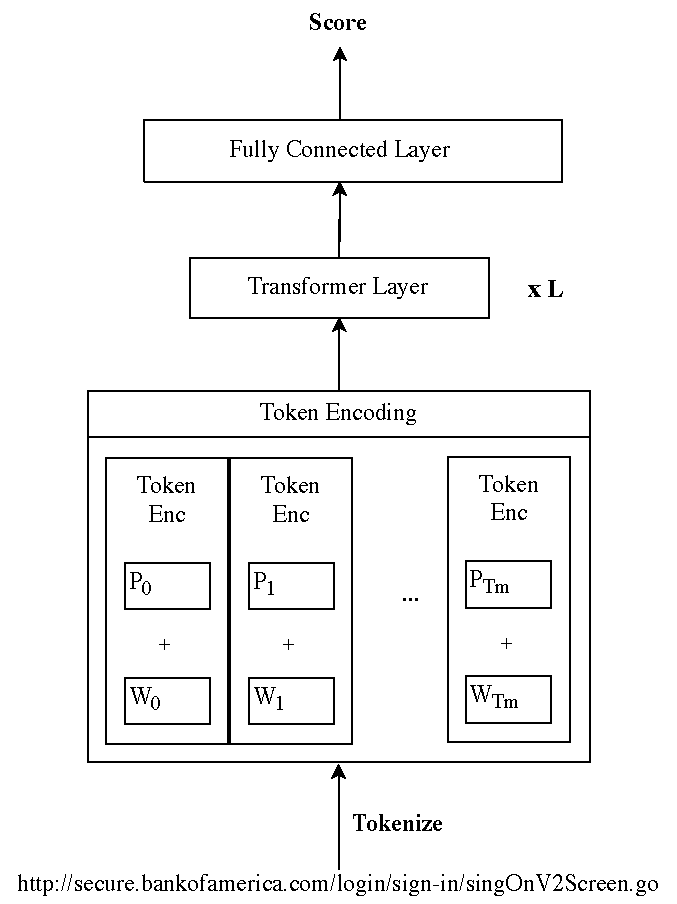
\includegraphics[width=0.4\linewidth]{urltran/figures/TransformerModel}
	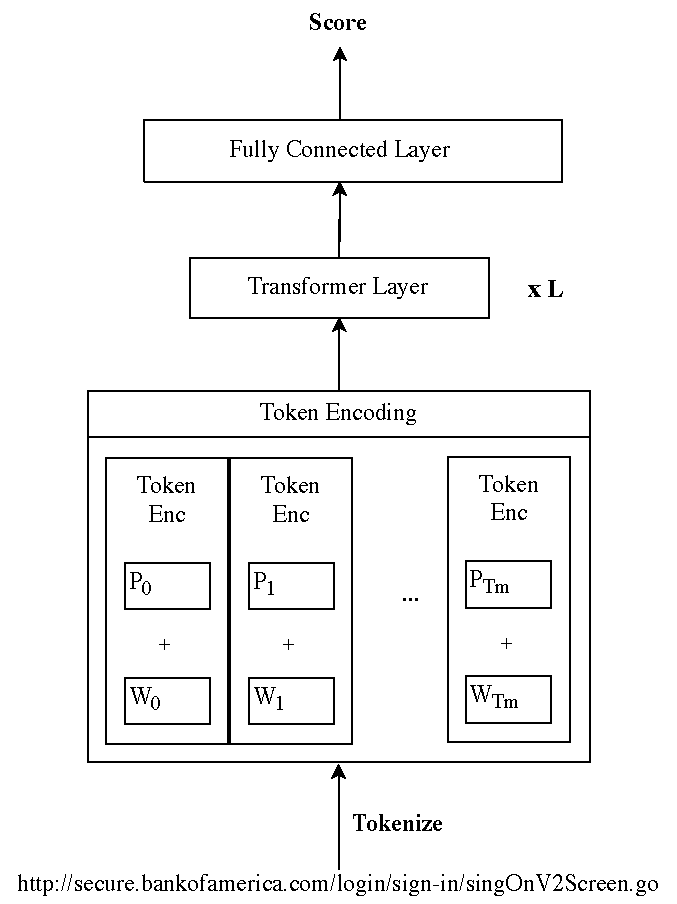
\includegraphics[width=0.4\linewidth,alt={Block diagram showing the inputs, tokenization, layers, and output of model.}]{urltran/figures/TransformerModel}
	\caption{\URLTranSys phishing URL detection model.}
	\label{fig:urltran:transformer}
\end{figure}
%\tagmcend\tagstructend
In the following sections, we first provide briefly summarize the transformer model architecture, followed by the training tasks used to train the model, and end with a description of the adversarial settings under which the best \URLTranSys model is evaluated and then trained with adversarial examples to improve its robustness.

\subsection{Architecture}
We describe the tokenization schemes and overall architecture for classification in this section, skipping a detailed description of transformer models for brevity.
Interested readers can review the transformer~\citep{vaswani2017attention}, BERT~\cite{devlin2019bert}, or RoBERTa~\citep{liu2019roberta} papers for details of the internal structure of transformer layers.

\subsubsection{Tokenization}
\label{sec:urltran:architecture:tokenization}
%
The raw input to the \URLTranSys model is the URL, which can be viewed as a text sequence.
The first step in the phishing URL detection task involves converting this input URL into a numerical vector which can be further processed by a classic machine learning or deep learning model.
Previous URL detection models~\citep{blum2020lexical} extracted lexical features by first splitting the URL with a set of important delimiters (e.g., `=', `/', `?', `.', ` ') and then creating a sparse binary features based on these tokens.
Recent deep learning-based URL detection models~\citep{le2018malicious,tajaddodianfar2020texception} instead include separate word-level and character-level CNNs where the character-level CNNs span different lengths of character subsequences.

Instead of these approaches, we experiment with multiple subword tokenization schemes in \URLTranSys.
Subword models have seen increased adoption in different tasks in NLP, including machine translation~\citep{sennrich2016neural}, word analogy~\citep{bojanowski2017enriching}, and question answering~\citep{zhang2019effective}.
Using subword models helps balance between the tradeoffs of using full-length words for each token (leading to fewer tokens required per input but a large token vocabulary) and character-based models (more tokens required per input but a smaller token vocabulary).
%allowing more input to be processed by a fixed-length model, 
%Using a subword model can provide morphological insights to improve inference.
For example, a full-length model would consider `bankofamerica' and `bankofcanada' as completely unrelated tokens, whereas a subword model can recognize the shared subword `bank' to correlate URLs belonging to the two banks.
Frequently occurring character substrings tend to correspond to subwords; common prefixes and suffixes can also provide relevant information.
%while being more robust to polymorphic attacks.
In particular, for fine-tuned \URLTranSysb and \URLTranSysr, we use the corresponding existing word piece~\citep{wu2016googles,devlin2019bert}  and Byte Pair Encoding (BPE) models~\citep{ratdford2019gpt2,liu2019roberta}, respectively.
In addition to these, we create custom character-level and byte-level BPE vocabularies using the training URL data to have a domain specific vocabulary for \URLTranSysc.
We test two different vocabulary sizes, 1K and 10K.
We tested  both sentence piece and BPE tokenization schemes in our models.
%as they attempt to find a balance of using both character substrings and full words and can capture unexpected unicode characters using their byte-level decomposition.


The BPE models first break the $m^{th}$ URL, $u_m$, into a sequence of text tokens, $\mathbf{TOK}_m$, where the individual tokens  may represent entire words or subwords~\citep{schuster2012japanese,sennrich2016neural,wu2016googles}.
Following the notation in~\cite{devlin2019bert}, the token sequence is formed as:
\begin{equation}
	\begin{split}
		& \mathbf{TOK}_m = \text{Tokenizer}(u_m)\\
	\end{split}
\label{eq:urltran:tok}
\end{equation}
%\end{comment}
\noindent where $\mathbf{TOK}_m$ is of length $T_m$ positions and consists of individual tokens ${Tok}_m^t$ at each position index $t$.
%${Tok}_t$ is an individual token generated from the $m^{th}$ URL generated by the wordpiece model.
For example, the BERT wordpiece token sequence generated from the URL of a popular banking login page,\\
\mbox{\small{$u_m$ = secure.bankofamerica.com/login/sign-in/signOnV2Screen.go}} \\
 is shown in Table~\ref{tab:urltran:boa}. The wordpiece model includes special text tokens specified by (\#\#) which build
 upon the previous token in the sequence. In the example in Table~\ref{tab:urltran:boa}, `\#\#of' refers to the continuation from s
 token (`bank'), and helps distinguish from the more common  separate token `of'.

\begin{table}
\centering
\resizebox{\linewidth}{!}{
\begin{tabular}{ll}
\hline
URL ($u_m$) & secure.bankofamerica.com/login/sign-in/signOnV2Screen.go \\
\hline
Token Sequence ($\mathbf{{TOK}_m}$) & \{ `secure', `.', `bank', `\#\#of', `\#\#ame', `\#\#rica', `.', `com', `/', `log', `\#\#in', `/', \\  & `sign', `-', `in', `/', `sign', `\#\#on', `\#\#v', `\#\#2', `\#\#screen', `.', `go' \} \\
  \hline
\end{tabular}
}
\caption{Example of the wordpiece token sequence extraction from a popular banking web page.}
\label{tab:urltran:boa}
\end{table}

\subsubsection{Classifier}
%
The final encoding produced by the transformer model can be used for a variety of downstream NLP tasks such
as language understanding, language inference, and question answering, and text classification.
We use the transformer embeddings for two tasks: pre-training masked language models, and fine-tuning for classification of phishing URLs.
Both of these tasks require a final representation layer which can be applied to multiple tokens for masked token prediction, and a pooled representation for classification.
The transformer models that we train use a single, dense two-class classification layer, which is applied to a special pooled token (`\texttt{[CLS]}') for classification. A dense layer having an output size equal to the size of the vocabulary of the tokenizer (\texttt{vocab\_size}) classes is used for predicting the masked token for the masked language modeling task during pre-training:

\begin{align}
	s_m = \sigma(\rmW_{p} \rvx_m^0 + \rvb_p) \label{eq:urltran:denseout}\\
	\rvs_m^t = \bm{\sigma} (\rmW_{v} \rvx_m^t + \rvb_v) \label{eq:urltran:denseword}
    %\label{eq:dense}
\end{align}

\noindent  In~(\ref{eq:urltran:denseout}), $\rmW_{p}$ and $\rvb$ are the weight matrix, bias vector respectively, for the final
dense linear layer for predicting the phising label.
$\sigma$ is the softmax function and 
 $s_m$ is the
score which predicts if the URL $\mathbf{u}_m$ corresponds to a phishing web page when performing classification.
Similarly, in~(\ref{eq:urltran:denseword}),
$\rvs_m^t, t \in [n]$ are 
 the sequence of masked token probability score vectors when performing masked language modeling for input token $\rvx_m^t$ computed using the softmax function $\bm{\sigma}$, with weight matrix $\rmW_{v}$ and bias vector $\rvb_v$.
 We now describe how input tokens are modified for masked language modeling and fine tuning.

\subsection{Training}
%
\subsubsection{Masked Language Modeling (MLM)}
The MLM task is commonly used to perform pre-training for transformers~\cite{devlin2019bert,liu2019roberta}. In this task, a random subset of tokens is replaced by a special `\texttt{[MASK]}' token.
 The training objective for the task is the cross-entropy loss corresponding to predicting the correct tokens at masked positions.
 The intuition for using this task for URLs is that specific query parameters and paths are generally associated with non-phishing URLs and therefore predicting masked tokens would help to uncover these associations.
 Similar intuitions derived from the cloze task~\cite{taylor1953cloze} motivate the usage of MLMs for pre-training natural language models.
Following the MLM hyperparameter settings for BERT, we selected 15\% of the tokens sampled uniformly for masking, of which 80\% are replaced, 10\% were left unchanged, and 10\% were replaced by a random vocabulary token at each iteration.
We used dynamic masking~\cite{liu2019roberta}, i.e., different tokens masked from the same sequence across iterations.
 Only the training subset of the full dataset was used for pre-training to prevent any data leakage. 

 \subsubsection{Fine Tuning}
 For \URLTranSysb and \URLTranSysr, we initialized all the parameters using the pretrained weights provided for BERT by \citet{devlin2019bert} and RoBERTa by \citet{liu2019roberta} respectively.
 For \URLTranSysc, we first pretrain each model using the MLM pretraining task and use the learned weights as initialization values.
 Next, each \URLTranSys model, is trained
 using a second ``fine-tuning'' task using the error backpropagated from the URL classification task.
 We used the Adam~\cite{kingma2014adam} optimizer with cross-entropy losses to train each model.
 
 \subsection{Adversarial Attacks and Data Augmentation}
 \label{sec:urltran:adv_attack}
%\pmcomment{Potentially discuss covariate shift here?}
 
\textbf{Threat Model}
%\pmcomment{Consider rewording this seciton}
The approach we use for generating data for an adversarial attack includes generating separate augmented training, validation and test datasets based on their original dataset.%~\cite{Goodfellow2014}.
For each URL processed in these datasets, we generate
a random number. If it is less than 0.5, we augment the URL, or otherwise, we include it in its original form. For URLs which are to be augmented,
we modify it using either a homoglyph attack, a compound attack or parameter reordering with equal probability. If a URL has been augmented,
we also include the original URL in the augmented dataset. 

The threat model for \URLTranSys allows for the attacker to create any phishing URL including those which employ domain squatting techniques. In its current form, \URLTranSys is protected against homoglyph and compound word attacks through dataset augmentation.
However, any domain squatting attacks can also be simulated and included in the augmented adversarial training, validation, and test sets. 
In addition, a larger number of adversarial training examples can be directed at more popular domains such as https://www.bankofamerica.com that may be a target of attackers.
We assume that inference can be executed by the countermeasure system prior to the user visiting the unknown page. 
This can be done by the email system at scale by evaluating multiple URLs in parallel. In our evaluation, we found that \URLTranSys requires 0.36096 milliseconds per URL on average which is a reasonable amount of latency.
 
 \textbf{Adversarial Testing}
 Data augmentation using invariants, contextual replacement, and reward-based learning has been used to improve classifiers in the text domain~\citep{kobayashi2018contextual,hu2019learning}.
 These can be extended to augment data in the URL domain.
 Phishing URL attacks can occur on short-lived domains and URLs which have small differences from existing, legitimate domains.
 We simulate two attack scenarios by constructing examples of such adversaries based on modifying benign URLs.
 Note that these generated domains do not actually exist in the pre-existing training and testing data, but are based upon frequently observed phishing attack patterns.
 We also utilized a reordering-based augmentation, which is used is used to generate benign perturbations for evaluating robustness of adversarially trained models.

 \subsubsection{Homoglyph Attack}
We generated domains that appear nearly identical to legitimate URLs by substituting characters with other unicode characters that are similar in appearance.
This attack strategy is commonly referred to as a \textit{homoglyph attack}~\cite{ji2018deepwordbug,yerima2020high}, and
we implement this strategy using the \texttt{homoglyphs}\footnote{https://pypi.org/project/homoglyphs/} python library.
In particular, given a URL, we first extract the domain.
For a randomly selected character in the domain, we check for one unicode (utf-8) Latin or Cyrillic character that is a homoglyph for it. 
For each perturbed URL, we selected a random character to perturb and generated the associated URL, labeled as a phishing URL.
We replaced the character by its homoglyph to construct a new URL.
%We only perturb one character to minimize the probability that such a URL would we be identified as phishing by the user.
%The URLs generated from this strategy are labeled as phishing.

\subsubsection{Compound Attack}
An alternative way to construct new phishing URLs is by splitting domains into sub-words (restricted to English) and then concatenating the sub-words with an intermediate hyphen.
For example, `bankofamerica.com' $\rightarrow$ `bank-of-america.com'.
To implement this, we leveraged a popular dictionary used by multiple spell check programs, the \texttt{enchant} dictionary\footnote{https://pypi.org/project/pyenchant/}.
Consider a URL with domain $d$ having $|d| = n$ characters.
Let $\gD$ denote the \texttt{enchant} English dictionary.
Let $C(d, i, j)$ denote the function that returns True if $d[i \dots j]$ can be split into one or more parts, each of which is a word in the dictionary $\gD$.
The compound word problem can be formulated recursively as
\begin{align}
	C(d, i, j) =
	\begin{cases}
		\text{True}, & d[i \dots j] \in \gD\\
		\text{True} & \exists k, C(d, i, k) \text{ and } C(d, k+1, j)\\
		\text{False} & \text{otherwise}
	\end{cases}
\end{align}
Using this recursive definition, we implemented a dynamic programming algorithm that can compute whether a domain can be split and the corresponding splits.
%\pmcomment{Maybe add the dynamic program algorithm here, and talk about the computational complexity?}
These splits are then concatenated with hyphens between the discovered words.
Note that the base case check  $d[i\dots j] \in \gD$ is performed in a case insensitive manner to ensure that the dictionary checks do not miss proper nouns.

\newcommand{\permuteSys}{PermuteURL\xspace}
\subsubsection{Parameter Reordering}
Forms of permutation=based denoising have shown improvements for langauge modeling~\cite{lewis2020bart} and machine translation~\cite{lample2018unsupervised}.
We adapt these intuitions into the phishing URL domain.
As the query parameters of a URL are interpreted as a key-value dictionary, this augmentation incorporates permutation invariance. 
An example of a URL and permutation is provided in Figure~\ref{fig:urltran:permute_url}.
We use this approach to generate benign examples.
Reordering the parameters still results in a valid URL, i.e., parameter reordering does not represent a phishing attack, and therefore we do not modify the label.
\begin{figure}
	\centering
	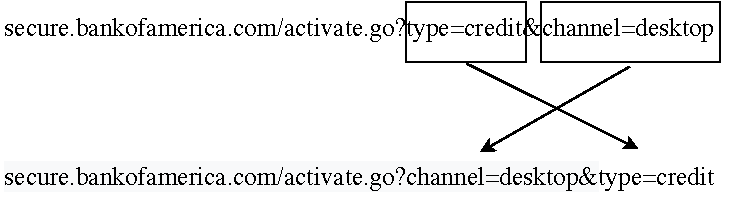
\includegraphics[width=0.75\linewidth,alt=Example of GET paramter reordering for a URL.]{urltran/figures/PermuteURL}
	\caption{An example of parameter reordering}
	\label{fig:urltran:permute_url}
\end{figure} 


 

\section{Evaluation}
\label{sec:urltran:eval}
%
We now present the numerical evaluation of the different approaches presented in the previous sections.
Thereafter, we compare \URLTranSys to several recently proposed baselines.
We also report the model's training and inference times.
Finally, we analyze the robustness of the model \textit{adversarial test}  URLs.


\noindent\textbf{Setup:}
In our experiments, we set the hyperparameters for previously published models according to their settings in the original paper.
For evaluating \URLTranSysc, we vary the number of layers between $\{3, 6, 12\}$, vary the number of tokens per input URL sequence between $\{128, 256\}$.
We use both a byte-level and character-level BPE tokenizer with 1K- and 10K-sized vocabularies.
We randomly pick 15 hyperparameter combinations among these settings and present the results for these.
The Adam optimizer~\citep{kingma2014adam} is used in both pre-training and fine-tuning, with the triangular scheduler~\citep{smith2017cyclical} used for fine-tuning.
The hyperparameter settings for all models are provided in Section~\ref{sec:urltran:hyper}.
All training and inference experiments were conducted using PyTorch~\citep{pytorch} version 1.2 with NVIDIA Cuda 10.0 and Python 3.6.
The experiments were performed by extending the HuggingFace and Fairseq PyTorch implementations found on GitHub~\citep{huggingface,fairseq}.
Given the large class imbalance, accuracy is a poor metric of model performance.
To supplement accuracy, we evaluated all the models using the true positive rate (TPR) at low false positive rate (FPR) thresholds. 
We used the receiver operating characteristics (ROC) curve to compute this metric.


\noindent\textbf{Baselines:}
To evaluate the performance of our models, we compared them to two baseline phishing URL detection models: URLNet and Texception. URLNet~\citep{le2018malicious} is a CNN-based model which was recently proposed for the task of detecting URLs which identify malicious web sites. 
For comparison purposes, we trained and tested the URLNet model for the detection of phishing URLs.
Texception~\citep{tajaddodianfar2020texception} is another deep learning URL detection model for the task of identifying phishing URLs. 
Note that \citet{tajaddodianfar2020texception} compared Texception to a Logistic Regression-based model and found that Texception offered better performance.
Thus, we did not repeat that baseline experiment in this work.

\subsection{End-to-end Training}
%\noindent\textbf{\URLTranSysc.}
Transformers typically require large amounts of pre-training data (e.g., BERT~\citep{devlin2019bert} used a corpus of  $\approx$ 3.3 B tokens).
However, this data is derived from text articles, which are structured differently from URLs.
We trained the \URLTranSysc model based solely on the URL data found in our datasets to compare the results of finetuning using BERT (\URLTranSysb) and RoBERTa (\URLTranSysc) pretrained models to models pretrained only on in-domain URL data. 
The difference in dataset size and data domain make it important to understand the impact of different hyperparameters used when training transformers from scratch.
We compared runs across different hyperparameters on the basis of area under ROC (AUROC) and TPR@0.01\% FPR.
Figure~\ref{fig:urltran:pretrain_scratch} demonstrates that the training is not very sensitive to sequence length. 
Smaller byte-level vocabularies tend to be better overall, but at low FPR, the difference is not significant.
Finally, we found that the 3 layer model generalized the best.
We hypothesize that the better performance of the model with fewer layers is because of limited pre-training data.%\todo{pre-training vs pretraining consistent}
In the next few sections, we validate this hypothesis by evaluating fine-tuned model (\URLTranSysb, \URLTranSysr) that are tuned on a larger dataset.

\begin{figure}
\begin{subfigure}{0.8\linewidth}
	\centering
    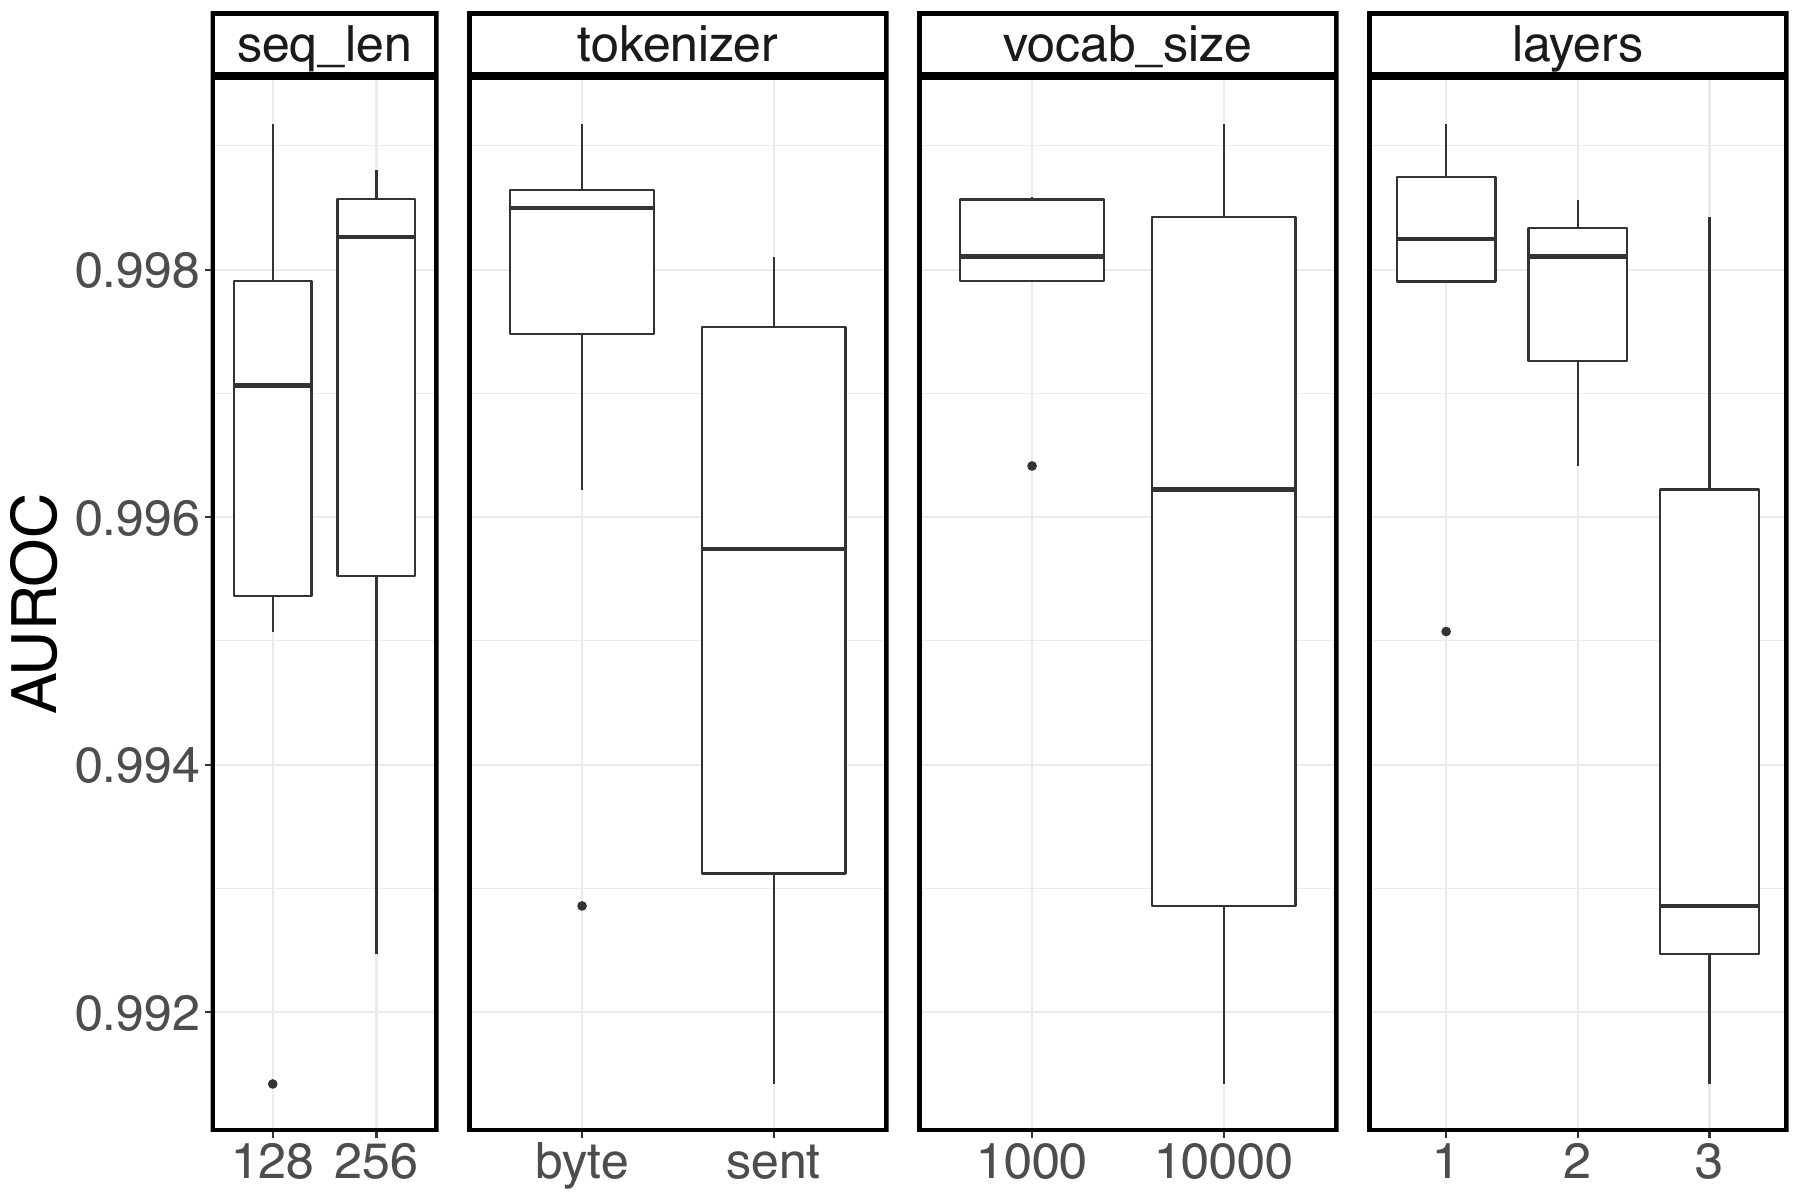
\includegraphics[width=0.95\linewidth,alt={Box plots for area under ROC comparison for different seq len, tokenizers, vocab size, and layers.}]{urltran/figures/roc_hyperparams.png}
\caption{Area under ROC vs hyperparameters}
\label{fig:urltran:pretrain_scratch:roc}
\end{subfigure}
\begin{subfigure}{0.8\linewidth}
	\centering
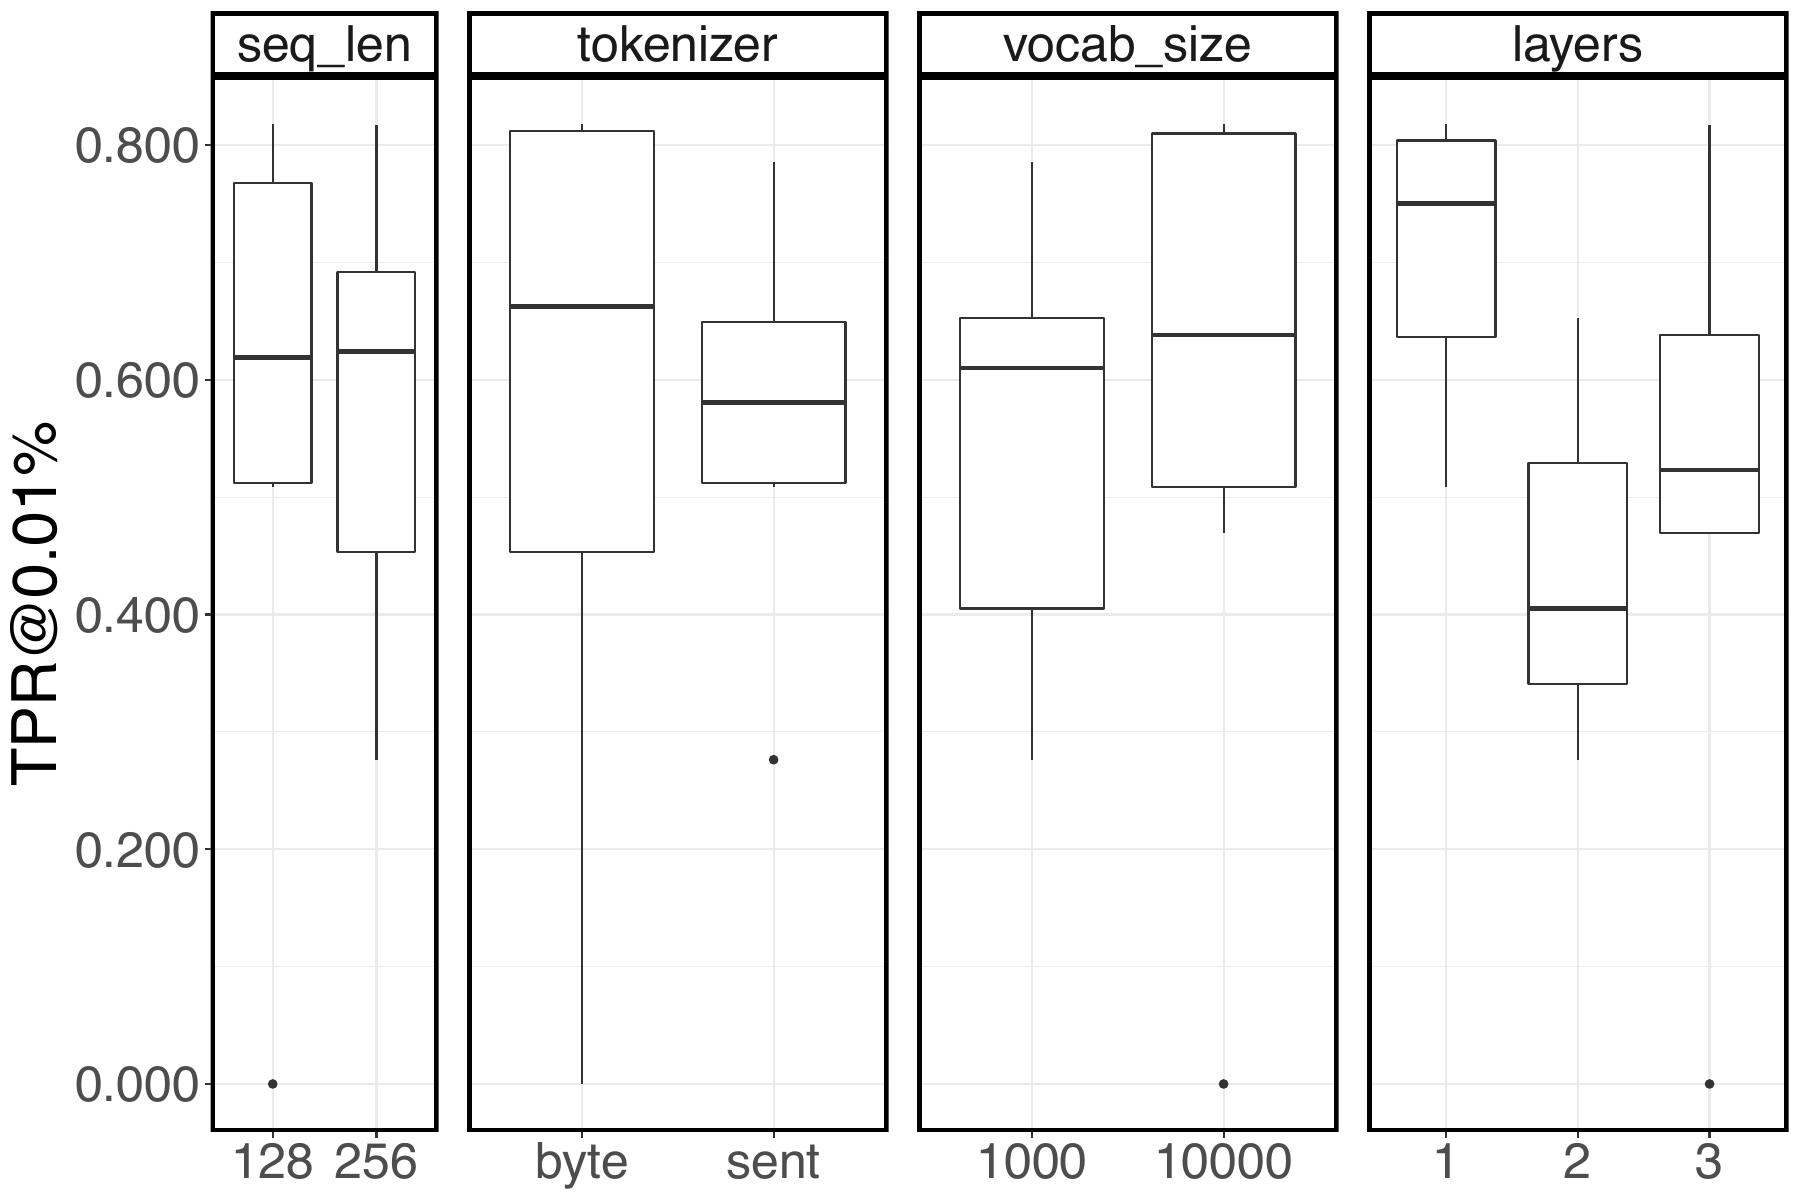
\includegraphics[width=0.95\linewidth,alt={Box plots for TPR@FPR=0.01\% comparison across different seq len, tokenizers, vocab size, and layers.}]{urltran/figures/tpr_0.01_hyperparams.png}
\caption{TPR@FPR = 0.01\% vs hyperparmeters}
\label{fig:urltran:pretrain_scratch:tpr}
\end{subfigure}
\caption{Variance in quality of \URLTranSysc across different hyperparameter settings}\
\label{fig:urltran:pretrain_scratch}
\end{figure}


\subsection{Numerical Evaluation}


\begin{figure}
    \centering
	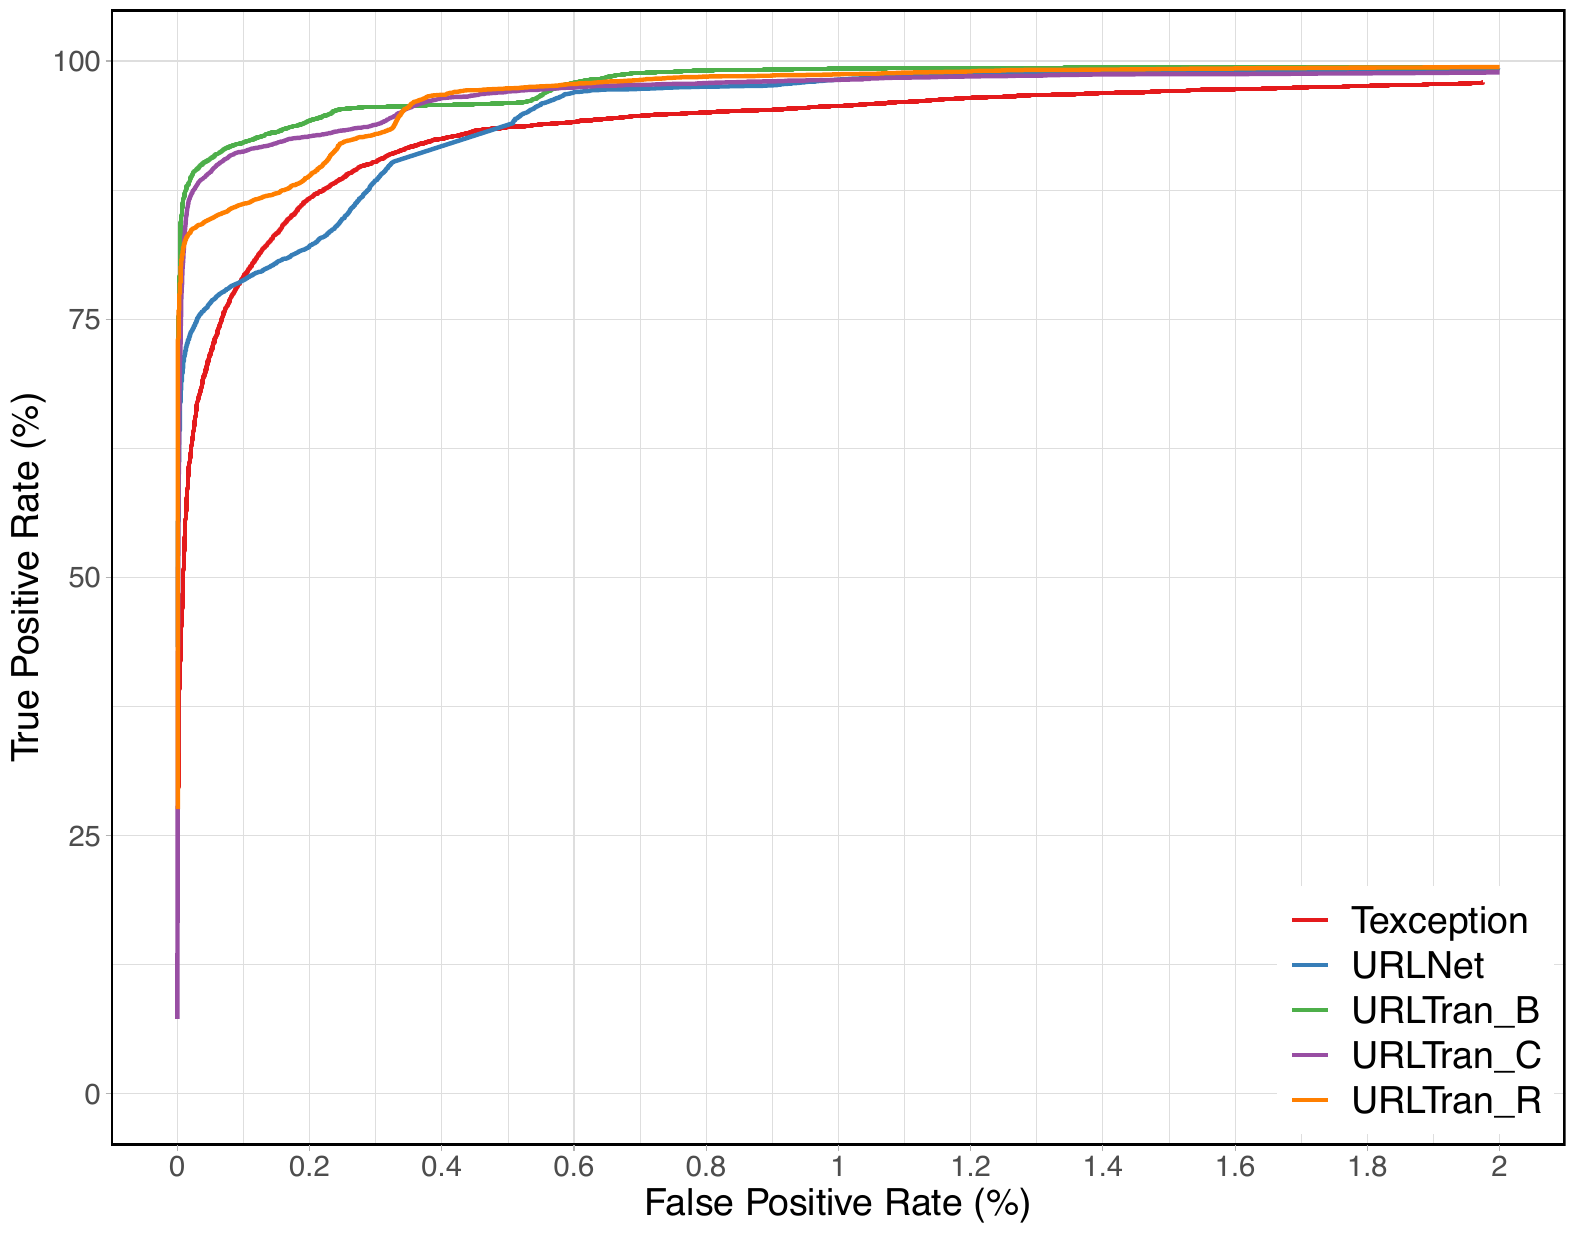
\includegraphics[width=0.7\linewidth,alt={ROC curev indicating impromvents of our model over baseline models upto a maximum of 2\% FPR}]{urltran/figures/roc_0_02_R.png}
	\caption{Receiver operating characteristic curve indicating the performance of the \URLTranSys and several baseline models zoomed into a maximum of 2\% false positive rate.}
	\label{fig:urltran:transformer2}
\end{figure}

\begin{figure}
    \centering
	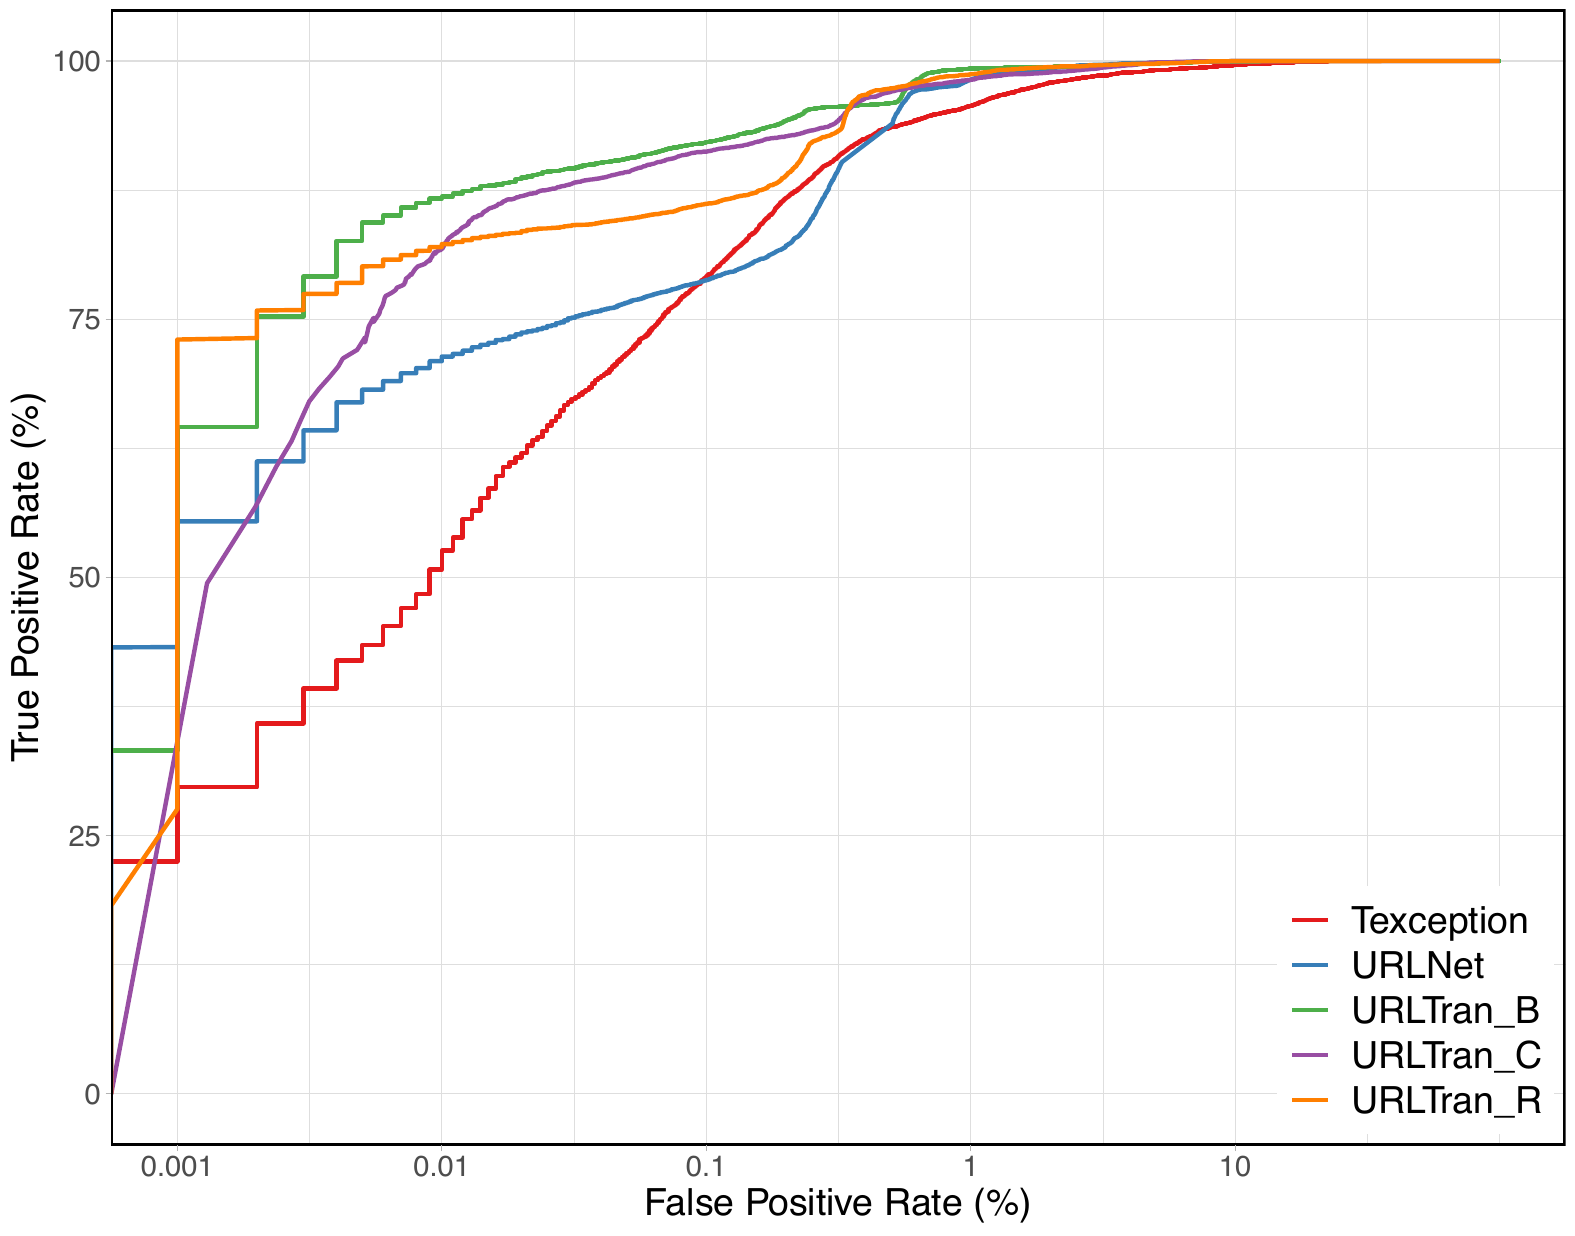
\includegraphics[width=0.7\linewidth,alt={Zoomed in full ROC curve with a log x-axis.}]{urltran/figures/log_roc_R.png}
	\caption{Zoomed in receiver operating characteristic curve with a log x-axis.}
	\label{fig:urltran:log_transformer2}
\end{figure}



\noindent\textbf{Model Performance.}
We next analyzed the performance of the best parameters of all the proposed transformer variants.
To understand how these models compare at \textit{very low FPRs} where detection thresholds must be set to operate in a production environment, we first plotted the ROC curves on a linear x-axis zoomed into a 2\% maximum FPR in Figure~\ref{fig:urltran:transformer2}.
We also re-plot these ROC curves on a log x-axis in the semilog plot in Figure~\ref{fig:urltran:log_transformer2}.
These results indicate that all variants of \URLTranSys offer a significantly better
true positive rate over a wide range of extremely low FPRs. In particular, \URLTranSys matches or exceeds the TPR of URLNet for the FPR range of 0.001\% - 0.75\%.
The result is very important because phishing URL detection models must operate at very low FPRs (e.g., 0.01\%) in order to minimize the number of times the security service predicts that a benign URL is a phishing site (i.e., a false positive). In practice, the browser manufacturer selects the desired FPR and tries to develop new models which can increase the TPR for the selected FPR value.
Note that TPR@FPR is the standard metric commonly used both in production settings and in prior art such as Texception and URLNet.
In addition to the ROC curve analysis, we also summarize a number of key performance metrics in Table~\ref{tab:urltran:model-perf}, where `F1' is the F1 score, and `AUC' is the area under the model's ROC curve.
The proposed \URLTranSys model outperforms both Texception and URLNet for all of these metrics.
In particular, we note that  at an FPR
of 0.01\%, \URLTranSysb has a
TPR of 86.80\% compared to 71.20\% for URLNet and 52.15\% for Texception.

\begin{table}[ht]
\begin{center}
\resizebox{\linewidth}{!}{
\begin{tabular}{ccccccc}
\toprule
Model & Accuracy (\%) & Precision (\%) & Recall (\%) & TPR@FPR=0.01\% & F1 & AUC \\
\midrule
Texception & 99.6594 & 99.7562 & 99.6594 & 52.1505 & 0.9969 & 0.9977 \\
URLNet & 99.4512 & 99.7157 & 99.4512 & 71.1965 & 0.9954 & 0.9988 \\
\URLTranSysc & 99.5983 & 99.7615 & 99.5983 & 81.8577 & 0.9965 & 0.9992 \\
\URLTranSysr & 99.6384 & 99.7688 & 99.6384 & 82.0636 & 0.9968 & 0.9992 \\
\URLTranSysb & 99.6721 & 99.7845 & 99.6721 & 86.7994 & 0.9971 & 0.9993 \\
\bottomrule
\end{tabular}
}
\end{center}
\caption {Comparison of different performance metrics for \URLTranSys and the two baseline models.}
\label{tab:urltran:model-perf}
\end{table}


%\input{error}

\noindent\textbf{Training and Inference Times.}
The total time required to train the best \URLTranSysb model was 4:57:11 on an NVIDIA V100. Inference
required 0:10::44 to complete for an average of 0.36096 milliseconds per sample.


\begin{figure}
    \centering
	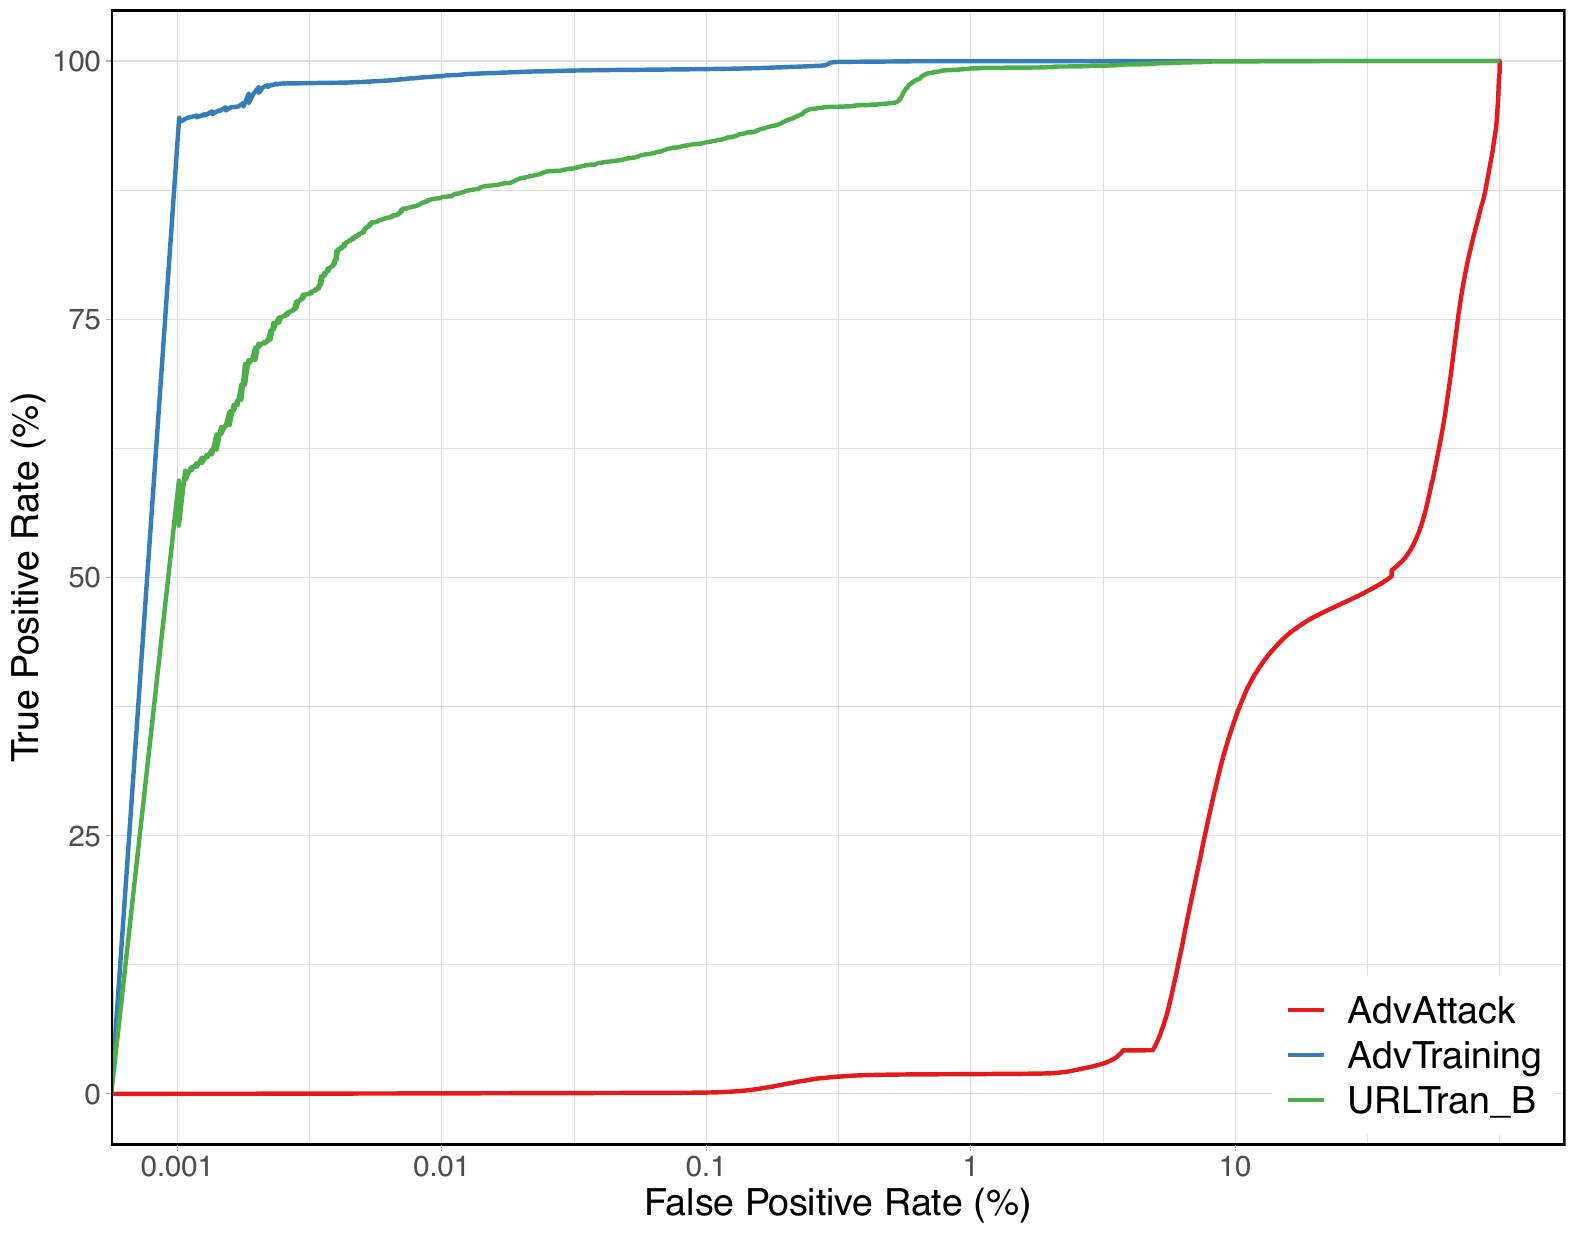
\includegraphics[width=0.7\linewidth,alt={ROC curve under adversarial attack and robustness after training with augmented data.}]{urltran/figures/log_roc_adv_R.png}
	\caption{ROC curve for \URLTranSysb when under adversarial attack, and adversarial robustness after augmented training}
	\label{fig:urltran:adversarial_roc}
\end{figure} 

\subsection{Adversarial Evaluation.}
To understand \URLTranSys's robustness to adversarial attacks, we first compared the low FPR regions of the ROC curve of the unprotected model tested with the original test set to the
test set which includes adversarial samples (AdvAttack) generated through the methods described in Section~\ref{sec:urltran:adv_attack} (Figure~\ref{fig:urltran:adversarial_roc}).
There is a significant drop in performance of \URLTranSysb when attacked with adversarial URLs.
As discussed previously (Section~\ref{sec:urltran:adv_attack}, \textit{adversarial testing} provides a mechanism to ensure that models can be made robust to attacks that follow known threat models.
We test this hypothesis by considering the scenario where attack strategies are incorporated into the training data (AdvTraining).
%\pmcomment{Another place where covariate shift can be referenced.}
On the addition of adversarial attack patterns to the training, the model is able to  the adapt to novel attacks, and even exceeded the performance of the non-adversarially trained version of \URLTranSys.
These results demonstrate that  creating adversarial can help models such as \URLTranSys adapt to unseen attacks.
Further, as new attack strategies are recognized (e.g., alternative homoglyph), a robust version of \URLTranSys can be trained to recognize similar patterns in unseen test data.

\section{Hyperparameter Settings}
\label{sec:urltran:hyper}
For replicability, this sectino provides the hyperparameter settings for the three variants of the proposed \URLTranSys model as well as those for two baseline models.
Tables~\ref{tab:urltran:URLNetParams} and~\ref{tab:urltran:TexParams} list the hyperparameters for the URLNet and Texception models that we use
as baselines in our study. The hyperparameter settings for the best performing \URLTranSysb model are provided in Table~\ref{tab:urltran:TransParamsBert}.
In addition, the best hyperparameter settings for the \URLTranSysr and \URLTranSysc are given in Tables~\ref{tab:urltran:TransParamsRoberta} and~\ref{tab:urltran:TransParamsCustVoc},
respectively.

\begin{table}
\centering
\footnotesize
\begin{tabular}{lc}
\toprule
Parameter & Value \\
\midrule
max\_len\_words & 200 \\
max\_len\_chars & 1000 \\
max\_len\_subwords & 20 \\
min\_word\_freq & 1 \\
dev\_pct & 0.001 \\
delimit\_mode & 1 \\
emb\_dim & 32 \\
filter\_sizes & {[}3,4,5,6{]} \\
default\_emb\_mode & char + wordCNN \\
nb\_epochs & 5 \\
train\_batch\_size & 128 \\
train\_l2\_reg\_lambda & 0.0 \\
train\_lr & 0.001 \\
\bottomrule
\end{tabular}
\caption{Hyperparameters used for URLNet.}
\label{tab:urltran:URLNetParams}
\end{table}


\begin{table}
\centering
\footnotesize
\begin{tabular}{clc}
\toprule
\multicolumn{2}{c}{Parameter} & Value\\
\midrule
\multirow{5}{*}{
\vtop{\hbox{\strut Characters}\hbox{\strut Branch}}
} & embedding dimension & 32 \\
 & number of blocks & 1\\
 & block filters & {[}2,3,4,5{]}\\
 & Adaptive MaxPool output & 32,32\\
 & maximum characters & 1000\\
\midrule
\multirow{5}{*}{
 \vtop{\hbox{\strut Words}\hbox{\strut Branch}}
} & embedding dimension & 32\\
 & number of blocks & 1\\
 & block filters & {[}1,3,5{]}\\
 & Adaptive MaxPool output & 32,16\\
 & maximum words & 50\\
\midrule
\multirow{6}{*}{
\vtop{\hbox{\strut FastText}\hbox{\strut Model}}
} & minimum words to include & 50\\
 & vocabulary size & 120000\\
 & window size & 7\\
 & n-grams & 2-6\\
 & embedding dimension & 32\\
 & epochs trained & 30\\
\bottomrule
\end{tabular}
\caption{Hyperparameters used for Texception.}
\label{tab:urltran:TexParams}
\end{table}

\begin{table}
\centering
\footnotesize
\begin{tabular}{lc}
\toprule
Parameter & Value \\
\midrule
  attention probs dropout prob & 0.1 \\
  hidden act & gelu \\
  hidden dropout prob & 0.1 \\
  hidden size & 768 \\
  initializer range & 0.02 \\
  intermediate size & 3072 \\
  layer norm eps & 1e-12 \\
  max position embeddings & 512 \\
  num attention heads & 12 \\
  num hidden layers & 12 \\
  type vocab size & 2 \\
  vocab size & 30522 \\
  bert model & bert-base-uncased \\
  max seq length & 128 \\
  train batch size & 32 \\
  learning rate & 2e-5 \\
  num train epochs & 10 \\
  \bottomrule
\end{tabular}
\caption{Hyperparameters  used for training the proposed Huggingface-based \URLTranSysb model.}
\label{tab:urltran:TransParamsBert}
\end{table}

\begin{table}
\centering
\footnotesize
\begin{tabular}{lc}
\toprule
Parameter & Value \\
\midrule
Number of Layers & 12 \\
Hidden size & 768 \\
FFN inner hidden size & 3072 \\
Attention heads & 12 \\
Attention head size & 64 \\
Dropout & 0.1 \\
Attention Dropout & 0.1 \\
Warmup Steps & 508 \\
Peak Learning Rate & 1e-4 \\
Batch Size & 2k \\
Max Epochs & 10 \\
Learning Rate Decay & Linear \\
Adam $\epsilon$ & 1e-6 \\
Adam $\beta_1$ & 0.9 \\
Adam $\beta_2$ & 0.98 \\
Gradient Clipping & 0.0 \\
Tokens per sample & 256 \\
\bottomrule
\end{tabular}
\caption{Hyperparameters used for fine-tuning the proposed Fairseq-based \URLTranSysr model.}
\label{tab:urltran:TransParamsRoberta}
\end{table}

\begin{table}
\begin{subtable}{0.45\linewidth}
    \footnotesize
    \centering
    \begin{tabular}{lc}
        \toprule
        Parameter & Value \\
        \midrule
        Number of Layers & 3 \\
        Hidden size & 768 \\
        FFN inner hidden size & 3072 \\
        Attention heads & 12 \\
        Attention head size & 64 \\
        Dropout & 0.1 \\
        Attention Dropout & 0.1 \\
        Tokens per sample & 128 \\
        Peak Learning Rate & 1e-4 \\
        Batch Size & 2k \\
        Tokenizer Type & Byte BPE\\
        Weight Decay & 0.01 \\
        Max Epochs & 30 \\
        \multirow{2}{*}{Learning Rate Decay} & reduce \\
         & on plateau \\
        LR Shrink & 0.5 \\
        Adam $\epsilon$ & 1e-6 \\
        Adam $\beta_1$ & 0.9 \\
        Adam $\beta_2$ & 0.98 \\
        Gradient Clipping & 0.0 \\
        Learning Rate & 1e-4 \\
        vocab size & 10000 \\
      \bottomrule
    \end{tabular}
\end{subtable} %
\begin{subtable}{0.45\linewidth}
    \footnotesize
    \centering
	\begin{tabular}{lc}
        \toprule
		Parameter & Value \\
        \midrule
		Learning Rate & 1e-4 \\
		Batch Size & 2k \\
		Max Epochs & 10 \\
		Learning  & \multirow{2}{*}{Linear} \\
		Rate Decay & \\
		Warmup ratio & 0.06 \\
		\bottomrule
	\end{tabular}
\end{subtable}
\caption{Hyperparameters used for pre-training (left) and fine-tuning (right) the proposed \URLTranSysc model.}
\label{tab:urltran:TransParamsCustVoc}
\end{table}

\section{Conclusion}
\label{sec:conc}
%
This work focused on the \textit{pre-deplyment} stage for building more adaptive models by incorporating \textit{adversarial testing}.
We have proposed a new transformer-based system called \URLTranSys whose goal is to predict the label of an unknown URL one which either references a phishing or a benign web page.
Transformers have demonstrated state-of-the-art performance in many natural language processing tasks, and the secnd objective of this work is to understand if these methods can also work well in the cybersecurity domain.
We demonstrated that transformers which are fine-tuned using standard BERT tasks and a BPE tokenizer also work remarkably well for the task of predicting phishing URLs.
%Instead of extracting lexical features or using CNNs kernels which span multiple characters and words, common in previously proposed URL detection models, our system used BPE tokenizers for this task. 
%Next, transformers convert the token sequence to an embedding vector which can then be used as input to a dense linear layer.
Results indicate that \URLTranSys was able to significantly outperform recent baselines, particularly over a wide range of very low false positive rates.
We also demonstrated that transformers can be made robust to novel attacks under specific threat models when we adversarially augment the training data used for training them. 

\endinput

\chapter{Auditing Fairness Online through Iterative Refinement}
\label{chp:avoir}

Machine learning algorithms are increasingly being deployed for high-stakes scenarios. 
A sizeable proportion of currently deployed models make their decisions in a black-box manner. 
Such decision-making procedures are susceptible to intrinsic biases, which has led to a call for accountability in deployed decision systems.
In this work, we focus on user-specified accountability of decision-making processes of black box systems.
Previous work has formulated this problem as run time fairness monitoring over decision functions.
However, formulating appropriate specifications for situation-appropriate fairness metrics is challenging.
We construct \AVOIRmethodname{}, an automated inference-based optimization system that improves bounds for and generalizes prior work across a wide range of fairness metrics.
\AVOIRmethodname{} offers an interactive and iterative process for exploring fairness violations aligned with governance and regulatory requirements.
Our bounds improve over previous probabilistic guarantees for such fairness grammars in online settings.
We also construct a novel visualization mechanism that can be used to investigate the context of reported fairness violations and guide users toward meaningful and compliant fairness specifications. 
We then conduct case studies with fairness metrics on three different datasets and demonstrate how the visualization and improved optimization can detect fairness violations more efficiently and alleviate the issues with faulty fairness metric design. 
A part of this work was included in a conference paper~\citep{maneriker2023online} presented at SIGKDD 2023, and the details of the implementation of AVOIR were included in a poster presented at the OSU TDAI Interdsciplinary Research Fall Forum 2023.


\section{Introduction}

Advanced analytics and artificial intelligence (AI), along with its many benefits, pose significant threats to individuals and the broader society.
\cite{Hirsch20} identify invasion of privacy; manipulation of vulnerabilities;  bias against protected classes; increased power imbalances;  error; opacity and procedural unfairness; displacement of labor;  pressure to conform, and intentional and harmful use as some of the key areas of concern.
A core part of the solution to mitigate such risks is the need to make organizations accountable and ensure that the data they leverage and the models they build and use are both inclusive of marginalized groups and resilient against societal bias.
Deployed AI and analytic systems are complex multi-step processes that can incorporate several sources of risk at each step.
At each of these stages, determining accountability in the decision-making of AI processes requires a determination of who is accountable, for what, to whom, and under what circumstances \citep{nissenbaum1996accountability,cooper2022accountability}. 
A more comprehensive overview of the mechanisms that can support accountability for the different stages of machine learning system design can be found in the work of \citet{cooper2022accountability}.
Our analysis centers on auditing fairness claims of mathematical guarantees associated with automated, black-box decision-making processes.
Governments worldwide are wrestling with different implementations of auditing regulations and practices to increase the accountability of decision processes.
Recent examples include the New York City auditing requirements for AI hiring tools~\citep{vanderford2022nybiaslaw}, European data regulation (GDPR~\citep{GDPR}), accountability bills~\citep{congress2023hr,algtransparency2022} and judicial reports~\citep{justice2018free}.
These societal forces have led to the emergence of checklists~\citep{mitchell2019model,sokol2020explainability}, metrics of fairness~\citep{verma2018fairness}, and recently, algorithms and systems that observe and audit the behavior of AI algorithms.
Such ideas date back to the 1950s~\citep{Moore1956}.
However, research has been sporadic until very recently, with the widespread use of AI-based decision-making giving rise to the vision of algorithmic auditing~\citep{Clavell20}.
In this work, we present a framework called \AVOIRmethodname{}\footnote{AVOIR in French means ``to have'', and this acronym reflects both our aspirational goal to achieve fairness in advanced analytics and AI but also reflects what is currently verifiable given a dataset, a model, and a fairness specification.}, for auditing and verifying fairness online.
%We present a framework for {\it Auditing and Verifying fairness Online through Iterative Refinement}~(\AVOIRmethodname{})
%
\AVOIRmethodname{} builds upon the ideas on distributional probabilistic fairness guarantees~\citep{albarghouthi2019fairness,bastani2019probabilistic}, generalizing them to real-world data. 
%Code for reproducing this work is available at \href{https://github.com/pranavmaneriker/AVOIR}{https://github.com/pranavmaneriker/AVOIR}.


\section{Related Work}
\label{sec:related}

There are a plethora of fairness criteria, and subtle changes in their definition can change the implications on decision-making~\cite{castelnovo2021zoo}.
Practitioners need support when selecting, designing, and guaranteeing fairness for deployed machine learning algorithms.
Prior work on fairness has helped develop nuanced notions and algorithms to help train more `fair' machine learning models.
These include group fairness measures such as inter alia, minimizing disparate impact~\citep{calders2009building,feldman2015certifying}, maximizing the equality of opportunity~\citep{hardt2016equality}
In contrast with group fairness notions, causal notions of fairness~\cite{kusner2017counterfactual} and individualized notions of fairness~\cite{dwork2012fairness} provide alternative statistical mechanisms for understanding discriminatory behaviors of automated decision systems.
\citet{thomas2019preventing} proposed the Seldonian Framework as a generic mechanism for model users to design algorithms that help train machine learning models that can regulate them against undesirable behaviors.
\citet{yan2022active} propose a query-efficient framework to audit an unknown function chosen from a known hypothesis class of decision-making functions.

We focus on the problem of detecting and diagnosing whether systems designed under any framework follow any prescribed regulatory constraints supported within the grammar of \AVOIRmethodname{}.
That is, we are agnostic to the framework; instead, we are interested in testing the adherence of models to specified criteria.
We use a probabilistic framework to verify this behavior.
Alternative frameworks such as the AI Fairness 360~\citep{bellamy2019AI}  provide mechanisms to quantify fairness uncertainty, though they are restricted to pre-supported metrics.
Uncertainty quantification~\citep{ghosh2021uncertainty,ginart2022mldemon} is an alternative mechanism to provide adaptive guarantees. 
However, existing work is designed for commonly used outcome metrics, such as accuracy and F1-score, rather than for fairness metrics. 
Justicia~\citep{ghosh2021justicia} optimizes uncertainty for fairness metrics estimates using stochastic SAT solvers but can only be applied to a limited class of tree-based classification algorithms.

Machine learning testing~\citep{mltesting} is an avenue that can expose undesired behavior and improve the trustworthiness of machine learning systems.
Prior work on fairness testing is most closely related to \AVOIRmethodname{}.
Fairness testing~\citep{galhotra2017fairness} provides a notion of causal fairness and generates tests to check the fairness of a given decision-making procedure.
Given a specific definition of fairness, Fairtest~\citep{fairtest} and Verifair (VF)~\citep{bastani2019probabilistic} build a comprehensive framework for investigating fairness in data-driven pipelines. 
%By auditing the system's fairness, a more balanced rule can be generated for future use.
Fairness-aware Programming (FP) \citep{albarghouthi2019fairness} combined the two demands of machine learning testing and fairness auditing to make fairness a first-class concern in programming. 
Fairness-aware programming applies a runtime monitoring system for a decision-making procedure with respect to an initially stated fairness specification.
The overall failure probability of an assertion is computed as the sum of the failure probabilities of each constituting sub-expression (using the union bound).
FP does not provide any specific mechanism for splitting uncertainty, and Verifair splits it equally across all constituent \textit{elementary subexpressions}.
Thus, assertion bounds for subexpressions in both FP and VF are split inefficiently compared to \AVOIRmethodname{}. 

\subsection{\AVOIRmethodname{}: Key Contributions}
\label{sec:contributions}

We now summarize our contributions vis-à-vis FP and Verifair.
(1) We build up \AVOIRmethodname{} in the framework of \textbf{confidence sets}~\citep{howard2021time} which enables the \textbf{adaptive optimization} of $\delta$ across subexpressions.
Note that FP provides examples with equal splits across two terms though it makes no specific prescription of splits.
Verifair splits uncertainty equally across all elementary subexpressions.
(2) The confidence sets framework allows us to move away from assuming a known data distribution or alternatively, fitting a density estimator over the population prior to fairness testing, required in Verifair.
(3) We augment the \textbf{bound propagation rules} to facilitate the online optimization process and allow propagation of constraints along with assertions at each iteration.
\todo{New contributions section.}
(4) We build an \textbf{inference engine} that supports automated inference of propagation rules for wide range of metrics.
In Section~\ref{sec:casestudy}, we provide examples of inference over specifications involving over two subexpressions, which are not possible without extending the implementations provided by previous work. 
As a baseline, we also implement bound inference rules from Verifair (denoted \AVOIRmethodname{}-VF).
(5) We support \textbf{interactive diagnosis} of fairness specification violations using visual cues associated with convergence of subexpressions.
We demonstrate the use of these cues to help drive the design of specifications in Section~\ref{sec:casestudy:adult}, which show how a user may have audited their original claim and refined mathematical bounds.
%More details about the differences referenced above are also available in Appendix~\ref{sec:appendix:contributions}.
\section{\AVOIRmethodname{} Framework}
\label{sec:theoretical}
%\pmcomment{1) Language spec, 2) inference of confidence rules 3) Define confidence sets/bounds, 4) Describe our algorithm, 5) show that our setting is a confidence set, 6) Prove that our method is better 7) Concrete Example}
\subsection{Language Specification}
\label{sec:theoretical:specification}

 
%Following~\cite{albarghouthi2019fairness}, for demonstrating its use, we build our framework as a library for specifying fairness criteria as decorators over python functions. 
We describe \AVOIRmethodname{}'s Domain Specific Language (DSL) used for specifying fairness metrics.
Concrete examples of implemented specifications in \AVOIRmethodname{}'s DSL are provided in Section~\ref{sec:casestudy}.
We focus on binary decision making functions; their outputs can be characterized by Bernoulli r.v.s.
Note that for such a Bernoulli r.v. $X$, $\E[X] = \Pr[X = 1]$ and hereafter, these are used interchangeably. 
Fairness specifications are implemented as decorators over decision functions.
Consider a decision function $f: X \rightarrow \{0, 1\}$, where $X = (X_1, \dots, X_k)$ denotes a real-valued input vector.  We use $R = f(X)$ to simplify the remainder of the definitions. 
\begin{itemize}
    \item  To support expressions beyond those that produce binary outputs, we use the grammar to construct Bernoulli r.vs. For example, a $\nu$-threshold based real-valued output, $R' = (R > \nu)$ and a multi-class output, for class $j$,  $R' = (R == j)$ correspond to Bernoulli r.vs.
\todo{Expanded definitions}
    \item  Expressions involving $R$ and $X_i$ act as the arguments \lstinline{<E>} to construct an \lstinline{<ETerm>}. For example  $\E[R > 0 | X_1 + X_2 > a]$ is an \textit{elementary subexpression} and an \lstinline{<ETerm>}
\end{itemize}
$c$ terms represent constant real values, used, for example, as bounds for expressions.
The grammar provided in Figure~\ref{fig:grammar} can be then used to construct various group fairness criteria.
%Nonparametric confidence sequences~\cite{howard2021time} can be used to extend these results to other r.vs.
%The grammar can be described using a Dmain Specific Language (DSL).
%\paragraph{Grammar for Specification DSL} 
%We start with the grammar used by prior work and enhance the grammar to simplify the expressions used for common fairness specifications. 
%Figure~\ref{fig:grammar} describes the full grammar. 
%\subsubsection{Modified Grammar}
We modified the grammar from prior work to include two additional operations. 
First, we added a \texttt{given} argument to the expectation term, which allows a user to specify conditional probabilities directly, in contrast to specifying it as a ratio of joint/marginal probabilities. 
 %In \citet{albarghouthi2019fairness}, conditional probabilities need to be specified as a ratio of the joint probability divided by the marginal probability of the conditional, i.e., $\E(A|B)$
 \begin{align*}
     \frac{\E(A \vee (B=b))}{\E(B=b)} \rightarrow \E(A, \mathtt{given}=(B=b))
 \end{align*}
 which is used to represent $\E[A|B=b]$, simplifying expressions used for group fairness specification.
Additionally, we add binary comparison operators $<, >, ==, !=$, which further simplifies the process of writing specifications. %\citet{albarghouthi2019fairness} only consider the $>$ operator as a part of their grammar. Thus, we build a more expressive grammar.

\subsection{Propagating Bounds}
\label{sec:theoretical:propagation}
%\paragraph{Inference and Optimization}
Generating the bounds for a specification requires propagating guarantees from elementary subexpressions.
Assuming that observed values for each \texttt{<E>} correspond to an underlying random variable $X$,
a probabilistic guarantee $\phi_X$ consists of an empirical estimate $\BarE[X]$, a concentration bound $\epsilon_X$, and a failure probability $\delta_X$, such that $\Pr[|\E[X] - \BarE[X]|\geq \epsilon_X] \leq \delta_X$.
We refer to expressions of this form as \textit{elementary} subexpressions.
A fairness specification will typically consist of multiple such elementary expressions, denoted as {\it compound} expressions.
For compound expressions, we must infer the implied guarantees that can be provided, with corresponding constraints.
%In addition, guarantees may require certain constraints to be satisfied.
Each inference rule corresponds to a derivation in the DSL grammar.
Inference rules have preconditions and postconditions that follow the general expression
\begin{align*}
 \frac{\bigcup \left\{r | r \in \{\phi, \psi, C \}\right\}}{\bigcup \left\{s | s \in \{ \phi, \psi, C \} \right\} }
\end{align*}
where $\phi$ denotes a claim for a subexpression, $\psi$ for a \verb|<spec>|, $\BarE$ and $\epsilon$ are the mean and concentration terms associated with a subexpression claim,  $C$ denotes a constraint. 
\todo{Updated the language to show the assumptions} 
For example, consider starting with the assumptions $X: (\BarE[X], \epsilon_X, \delta_X)$, $Y: (\BarE[Y], \epsilon_Y, \delta_Y)$.
Then we have
\begin{align*}
    |\E[X] \pm  \E[Y] - (\BarE[X] \pm \BarE[Y])| &= |(\E[X] - \BarE[X]) \pm  (\E[Y] - \BarE[Y])| \\
                                                  & \leq |\E[X] - \BarE[X]| + |\E[Y] - \BarE[Y]|\\
                                                  & \leq \epsilon_X + \epsilon_Y
\end{align*}
i.e., we can derive $X \pm Y: \left(\BarE[X] \pm \BarE[Y], \epsilon_X + \epsilon_Y, \delta_X + \delta_Y\right)$.
Some derivations also lead to rules that require constraints.
For instance, assume $X: (\BarE[X], \epsilon_X, \delta_X), \BarE[X] > c$. 
Then we have $\Pr[X < \BarE[X] - \epsilon_X] > 1 - \delta$
If we add the constraint that $\BarE[X] - \epsilon_X \geq c$, we have $\Pr[X < c] > 1 - \delta$, thus, 
\begin{align*}
    X: (\BarE[X], \epsilon_X, \delta_X) \implies \psi \equiv X > c: (T, \delta_X) \\
    \text{under the constraint } \{ \BarE[X] - \epsilon_X \geq c\}
\end{align*}
The full set of inference rules required for the DSL is provided in the appendix (\Figref{fig:inference}).
The implementation in \AVOIRmethodname{} follows these rules but can be extended to other rule inference templates that support the DSL.
We note that these rules extend the ones implemented by VeriFair (VF)\footnote{Verifair}~\citep{bastani2019probabilistic} with constraints that enable the optimizations required in \AVOIRmethodname{} (see Appendix~\ref{sec:appendix:inference-rules}). 
%\pmcomment{SP: Point to appendix?}

%\pmcomment{Keep constraint rules}




\subsection{Optimizing Bounds}
\label{sec:theoretical:optimization}


\subsubsection{\AVOIRmethodname{} Algorithm}

%\pmcomment{Move to algorithm environment}
%\pmcomment{reference MLP and interior point methods}
The pseudocode for the optimization procedure in \AVOIRmethodname{} is described in  the appendix (Algorithm~\ref{alg:method}).
The input to the algorithm is the reporting threshold probability $\Delta$ and a specification $\psi$.
We then infer a symbolic optimization problem is inferred corresponding to the failure probabilities and constraints derived from concentration bounds.
At each step, the \texttt{OBSERVE(X)} function is called with new observation of every \textit{elementary} subexpression and observed output.
The running mean and counts of observations are updated.
The final optimization problem \texttt{OPT} corresponding to each specification is a nonlinear constrained optimization problem.
We use the COIN-OR implementation of IPOPT~\citep{wachter2006implementation}, accessed though the Pyomo~\citep{hart2011pyomo} interface to solve this problem at each step.
If a solution is successfully found for \texttt{OPT}, the algorithm terminates, with the estimate for the specification having reached the required threshold.
If no solution is found, the estimates continue to be updated with $\delta_i = \Delta$ for each \textit{elementary} subexpression.
The main intuition behind the algorithm is to create a confidence sequence corresponding to the estimates at each time step.
The \texttt{OPT} corresponding to a specification:
\begin{align}
    \label{eq:optimization}
    \begin{split}
        &\min_{\delta_i} \sum_{i=1}^{n}\delta_i  \\
        \text{s.t. } &g_k(\delta_{1, \dots, n}, \BarE[X_1], \dots, \BarE[X_n]) \leq \epsilon_k\\
        & 0 \leq \delta_i \leq 1
    \end{split}
\end{align}
where $g_k$ and $\epsilon_k$ are the functions/bounds derived using the transformations carried out through the DSL inference rules (further details in Appendix~\ref{sec:appendix:inferrence-rules:opt}).


\begin{definition}
For $\delta \in (0, 1)$, a $(1-\delta)$ \textit{confidence sequence} is a sequence of confidence sets, usually intervals  $(\rm{CI}_t)_{t=1}^\infty,$, say $\rm{CI}_t \eqdef (L_t, R_t) \subseteq \sR$ satisfying a uniform convergence guarantee. After observing the $t$th unit, we calculate an updated confidence set $\rm{CI}_t$ for an unknown quantity of interest $\theta_t$ with the coverage property $\Pr(\forall t \geq 1, \theta_t: \theta_t \in \rm{CI}_t) \geq 1 - \delta$~\citep{howard2021time}.
\end{definition}

In this paper, we focus on the mean of r.v.s $\E[X]$ that constitute estimates for \textit{elementary} subexpressions as the quantities of interest. 
We use adaptive concentration inequalities to construct these confidence sequences.
Any adaptive concentration inequality that can be applied to a r.v. $X \in \{0, 1\}$ such that 
\begin{equation}
    \Pr[|\BarE_t[X] - \E[X]| \geq \epsilon(t, \delta)] \leq \delta
    \label{eq:adaptive-conc:general}
\end{equation}
can be used in \AVOIRmethodname{}. 
Here, $\BarE_t[X]$ denotes the empirical estimate of $\E[X]$ after the $t^{\rm{th}}$ observation.
For the purpose of comparison with previous work (eg., VF), we use the Adaptive Hoeffding Inequality~\citep{zhao2016adaptive}, which will be referred to as $\rm{AIN}$ hereafter.
%\pmcomment{SP: refer to $\rm{AIN}$ above but $\rm{AIN}$ below. Check and unify.}

\begin{theorem}
The sequence of estimates generated by \AVOIRmethodname{} form a confidence set.
\label{thm:conf-seq}
\end{theorem}
The proof follows from the fact that \AVOIRmethodname{} always estimates using a failure probability higher than that which is provided by $\rm{AIN}$, and hence applying a union bound ensures that the estimates are a confidence set. 
The full proof is provided in Appendix~\ref{sec:appendix:confseq}.

\begin{corollary}
The estimates for the overall specification $\psi$ form a confidence sequence converging to $\psi: (b, \Delta), b \in \{T, F\}$.
\end{corollary}
\begin{proof}
We initialize the main specification with the required failure probability $\Delta$. 
The termination condition requires $\sum \delta_i \leq \Delta$.
From Theorem~\ref{thm:conf-seq} we can infer that the confidence sequence corresponding to the termination achieves the required threshold $\Delta$, and therefore, is valid.
\end{proof}


\subsubsection{Improvements over Baseline}
In all prior work~\citep{albarghouthi2017fairsquare,albarghouthi2019fairness,bastani2019probabilistic}, $\delta_i$ for each \textit{elementary} subexpressions is set to $\Delta/n$, where $n$ is the number such term in the specification.
\todo{Introduce $A_\delta$ }
This simplification is carried out using the assumption $A_\delta \eqdef \delta_i = \delta_j \forall i, j$ for all \textit{elementary} subexpressions.
As we do not make this assumption, we can prove the following key theorem.

\begin{definition}
We define the specification stopping time $\gT$ for a confidence sequence as the smallest time $t$ such that, given a threshold $\Delta$ and a specification $\psi$, we can terminate any inference algorithm to claim that  $\Pr[\forall t \geq 1, \psi_t = \widehat{\psi}_\gT] \geq 1 - \Delta$, where $\widehat{\psi}_{\gT}$ is the estimate of $\psi$ at time $\gT$.
\end{definition}

\begin{theorem}
\label{theorem:better-stopping}
Given a threshold probability $\Delta$ for a specification $\psi$, let the stopping time for \AVOIRmethodname{} be $\gT$ and stopping time with the $A_\delta$ assumption be $\gT^+$. Then $\gT \leq \gT^+$
\end{theorem}
See Appendix~\ref{sec:appendix:optimality} for the proof.

%\pmcomment{Need to make this argument rigorous}


%\pmcomment{Write this proof replacing AH/Verifair with arbitrary $\rm{IN}$}

\paragraph{Concrete Example}
%\label{sec:theoretical:improvements:concrete}
%\pmcomment{Prior work makes assumptions of equality of unceertainty thresholds; as we do not make this assumption, which allows us to optimize over prior owrk.}
Consider a Bernoulli r.v $R$ corresponding to the output of a binary decision function, with $s$ being an indicator of class membership. 
Let $X = r \vee s$ and $Y = r \vee \neg s$ be r.vs corresponding to a positive decision for the majority and minority classes, respectively. 
Suppose we aim to estimate $\psi \eqdef X - Y < \epsilon_T$

\begin{figure}[ht]
\begin{subfigure}[b]{0.45\linewidth}
\resizebox{\linewidth}{!}{
    \begin{tikzpicture}
        \centering
        \begin{axis}[
                %xtick = \empty,    ytick = \empty,
                grid=both,
                xlabel = {$\delta_X$},
                %x label style = {at={(1,0)},anchor=west},
                ylabel = {$\delta_Y$},
                %y label style = {at={(0,1)},rotate=-90,anchor=south},
                y label style = {rotate=-90},
                axis lines=left,
                xmin=0.03, xmax=0.06,
                ymin=0.04, ymax=0.07,
                label style={font=\Large}
            ]
            \addplot[color=cb-rose,thick,smooth,domain=0:0.1]{x};
            \addlegendentry{$\delta_X = \delta_Y$}
            
            
            \addplot[name path=delta, color=cb-lilac,thick,smooth,domain=0:0.1,forget plot]{0.1-x};
            \path[name path=axis2] (0,0) -- (0.1,0);
            \addplot [
                thick,
                color=cb-lilac,
                fill=cb-lilac, 
                fill opacity=0.05,
                draw=cb-lilac
            ]
            fill between[
                of=axis2 and delta, soft clip={domain=0:0.1}
            ];
            \addlegendentry{$\delta_X + \delta_Y \leq 0.1$};
            
            
            \addplot[name path=constraint,color=cb-brown,smooth,thick,-,domain=0:0.1,forget plot] {24/exp((9/5)*(((0.2 - sqrt(2.6146 + 5*ln(24/x)/9)/(5*sqrt(62)))^2) * 310 - 2.46838))};
            \path[name path=axis3] (0,0.1) -- (1,0.1);
            \addplot [
                thick,
                color=cb-brown,
                fill=cb-brown, 
                fill opacity=0.05,
                draw=cb-brown
            ]
            fill between[
                of=constraint and axis3,
                soft clip={domain=0:0.1}
            ];
            \addlegendentry{$\epsilon_X + \epsilon_Y \leq 0.2$}
        \end{axis}
    \end{tikzpicture}}
        \caption{No solution exists with additional constraint $A_\delta: \delta_X = \delta_Y = \Delta/2$ - common assumption in prior work.}
        \label{fig:theoretical-example}
    \end{subfigure}
    \hfill
    \begin{subfigure}[b]{0.45\linewidth}
        \centering
        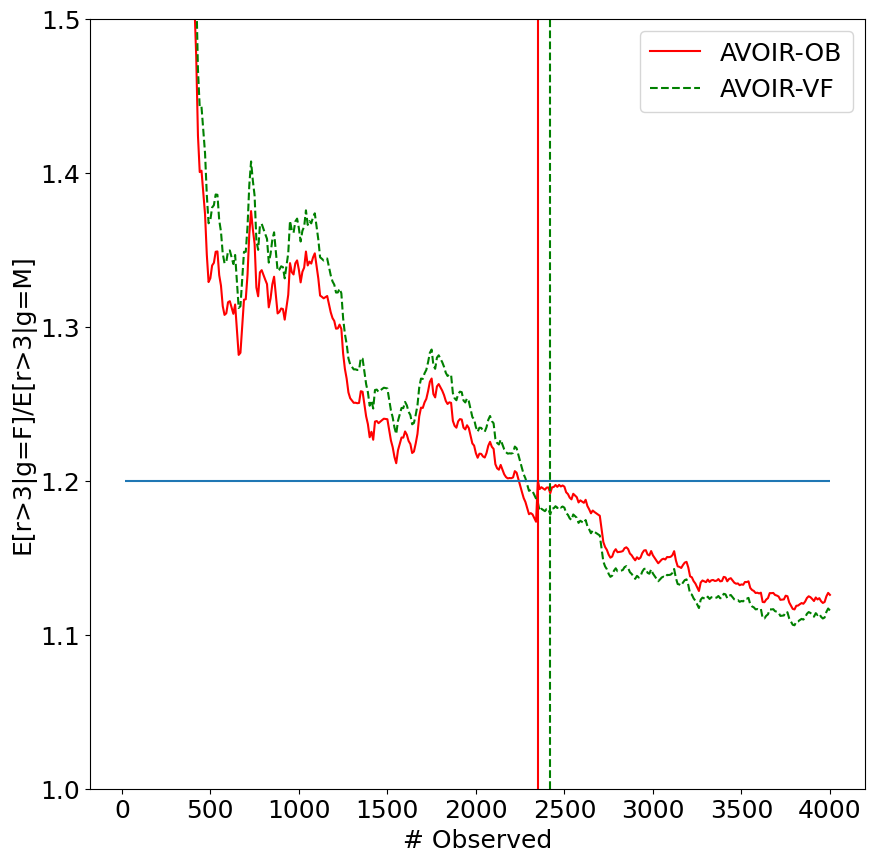
\includegraphics[width=\linewidth]{avoir/images/ratemyprofs.png}
        \caption{Bounds for first half of a gender-fairness specification generated by \AVOIRmethodname{}-OB and AVOIR-VF.}
        \label{fig:casestudy:rmp}
    \end{subfigure}
    \caption{\figleft{} \AVOIRmethodname{} finds a solution for a \textit{theoretical} scenario with $\delta_X + \delta_Y \leq \Delta$ under constraint $\epsilon_X + \epsilon_Y \leq \epsilon_T$ \figright{} For \textit{RateMyProfs}, a real-world dataset, the vertical lines show the step at which the methods can provide a guarantee of failure for the upper bounds with $\Delta <= 0.05$.}
    \label{fig:real-and-theoretical-examples}
\end{figure}


We demonstrate the improvements possible using our approach by instantiating this example with data. 
Suppose we want the upper bound of the failure probability $\Delta = 0.1$ for the specification.
Consider a set of observations such that $\BarE[X] = 0.8, n_X = 1550$ and $\BarE[Y] = 0.5, n_Y = 310$.
Figure~\ref{fig:theoretical-example} shows that no solution is feasible for the optimization problem with $A_\delta$.
However, \AVOIRmethodname{} can find a solution.
For the optimal solution, $\delta_2 \approx 2.35\delta_1$, which aligns with our intuition from section~\ref{sec:related} about allocating higher failure probability to terms with the majority of observations. 
The optimization problem inferred by \AVOIRmethodname{}:
\begin{align}
    \begin{split}
        &\min\limits_{\delta_X, \delta_Y}{\delta_X + \delta_Y} \\
        \text{s.t.  } &\epsilon_X + \epsilon_Y \leq \BarE[X] - \BarE[Y] - \epsilon_T \\
        &0\leq \delta_{X,Y} \leq 1
    \end{split}
\end{align}

%\pmcomment{Please point reader to location in appendix on proof.}


 

\begin{comment}
$\Pr[X] - \Pr[Y]  < \epsilon_T$. 
As $\Pr[X] = \E[X]$ for a Bernoulli r.v., this can be simplified as:
\begin{align*}
    \Pr[\Pr[X] - \Pr[Y] < \epsilon_T] &= \Pr[\E[X] - \E[Y] < \epsilon_T] \\
                                  &= 1 - \Pr[\E[X] - \E[Y] \geq \epsilon_T] \\
\end{align*}

Suppose $\BarE[X]_{(\epsilon_X, \delta_X)}$ and $\BarE[Y]_{(\epsilon_Y, \delta_Y)}$ be statistical guarantees derived for $X$ and $Y$ respectively. 
From the inference rules in Figure~\ref{fig:inference}, we have 
\begin{align*}
    \Pr[|(\E[X]-\E[Y]) - (\BarE[X] - \BarE[Y])| \geq \epsilon_X + \epsilon_Y] &\leq \delta_X + \delta_Y\\
    \implies \Pr[(\E[X]-\E[Y]) \geq \BarE[X] - \BarE[Y] -  (\epsilon_X + \epsilon_Y)] &\leq \delta_X + \delta_Y \\
    \implies \Pr[(\E[X]-\E[Y]) \geq \epsilon_T] &\leq \delta_X + \delta_Y
\end{align*}
where the last inequality follows if $\BarE[X] - \BarE[Y] - (\epsilon_X + \epsilon_Y) \geq \epsilon_T$
\end{comment}


%\pmcomment{TODO: replace the screenshot with a vector graphic from tikz}

\subsection{Visualization for Interactive Refinement}
Using our specification framework as a backend, we built an interactive application for analysis and refinement of specifications provided in our grammar.
Specifically, fairness specifications can be naturally parsed into a tree because of the structure of the grammar.
Each node of the tree represents some sub-expression in the syntax tree of the overall specification.
These nodes allow a user of \AVOIRmethodname{} to interactively audit and tune the specification definition.
To create the visualization, we use Vega~\citep{satyanarayan2015reactive}, a declarative JSON-based visualization grammar.
%To provide the evaluation plots, we need the evaluation values and the observations that they occurred at.
We log the estimates during runs of \AVOIRmethodname{} and then output the grammar in a tabular JSON-format that contains a row for each grammar element and its associated evaluations.
This tabular data is used by our Vega specification to produce the visualizations.
By selecting one of the nodes in the syntax tree, a user can see a plot of the evaluation values associated with the selected grammar element.
This allows for comparison of multiple grammar elements.
The ability to analyze and compare these evaluation values provides context surrounding specification violations, and assists the user in interacting with and deciding how to refine a specification
We provide a detailed example of how these interactions can help \AVOIRmethodname{} users choose an appropriate fairness metric in Section~\ref{sec:casestudy}.
%Given a user provided machine learning model, dataset, and specification the application simulates a stream of observations to the provided model.
%Following the simulation, a visualization is provided that represents the specification as a syntax tree where each node of the tree corresponds to an element of our grammar.
%Figures \ref{fig:casestudy:boston} and \ref{fig:casestudy:adult} show the visualization.
%Note that for each observation made by our machine learning model, the specification is evaluated to check for violations.
%Each grammar element that makes up the specification is evaluated as well, and thus each grammar element is associated with the value it evaluates to for a given observation.
%For the top level specification, \texttt{<spec>}, there is a boolean value associated with each observation, whereas an expectation term, \texttt{<ETerm>}, is associated with a real value.
%We call these plots evaluation plots and two can be observed at a time (see the plots on the right of figure \ref{fig:casestudy:boston}), each with shared scales along the horizontal axis which denotes observations over time.
%The case studies in section \ref{sec:casestudy} demonstrate the usefulness of the context provided by these visualizations.
%To create the visualization, we use Vega \cite{vega}, a declarative JSON-based visualization grammar.
%To provide the evaluation plots, we need the evaluation values and the observations that they occurred at.
%We log these values during the simulation our application runs, and then output the grammar in a tabular JSON-format that contains a row for each grammar element and it's associated evaluations.
%This tabular data is used by our Vega specification to produce the visualizations.
\begin{comment}
The app proceeds in multiple stages,
\begin{enumerate}
    \item First, a user selects a dataset of interest. We built support for two datasets, but our framework is generic enough for any arbitrary csv dataset.
    \item Following this choice, the input variables and output variable for a machine learning model must be specified.
    \item A machine learing model is then selected from a dropdown. We provide support for three models. However, this is for demonstration purposes only - the specification is agnostic to the choice of a machine learning model.
    \item Finally , a specification is input by the user of the app. On the press of a button, the model is trained and then evaluated on the selected dataset. The output monitored by the spec is passed off to the Vega module for further analysis.
\end{enumerate}
\end{comment}
\section{Evaluation}
\label{sec:casestudy}
In this section, we evaluate \AVOIRmethodname{}.variants through three real-world case studies.
Direct comparisons with existing work are impossible since no other work (to our knowledge) facilitates a general-purpose inference engine for online fairness auditing using arbitrary measures.
We can, however, implement VF's~\cite{bastani2019probabilistic} inference rules within \AVOIRmethodname{} (denoted as \AVOIRmethodname{}-VF).
Note that \AVOIRmethodname{}-VF sidesteps the assumptions of having a known data-generating distribution (made possible by \AVOIRmethodname{}'s reliance on confidence sets), making this variation a more practical and efficient algorithm. 
We denote \AVOIRmethodname{}-OB as the implementation that utilizes the abovementioned optimizations. 
Across the studies, the role of chosen threshold probabilities is similar to that of p-values in statistics.
Typical p-values tend to be $0.05$ and $0.1$, which we demonstrate in the RateMyProfs and COMPAS risk assessment study. 
In our case study of prior work~\cite{angwin2016machine}, we stick to the available definitions and thresholds used in the original analysis.
We expect that regulators will set the threshold probabilities on a case-by-case basis, e.g,, $0.15$ for illustration purposes in the adult income study.%, and we provide the adult income study with  $\Delta =0.15$ as an example.

%An important case study on the COMPAS dataset can be found in Appendix~\ref{sec:appendix:additional-case-studies}. 
\subsection{Rate My Profs}
\label{sec:casestudy:rmp}
\begin{figure}
    \centering
    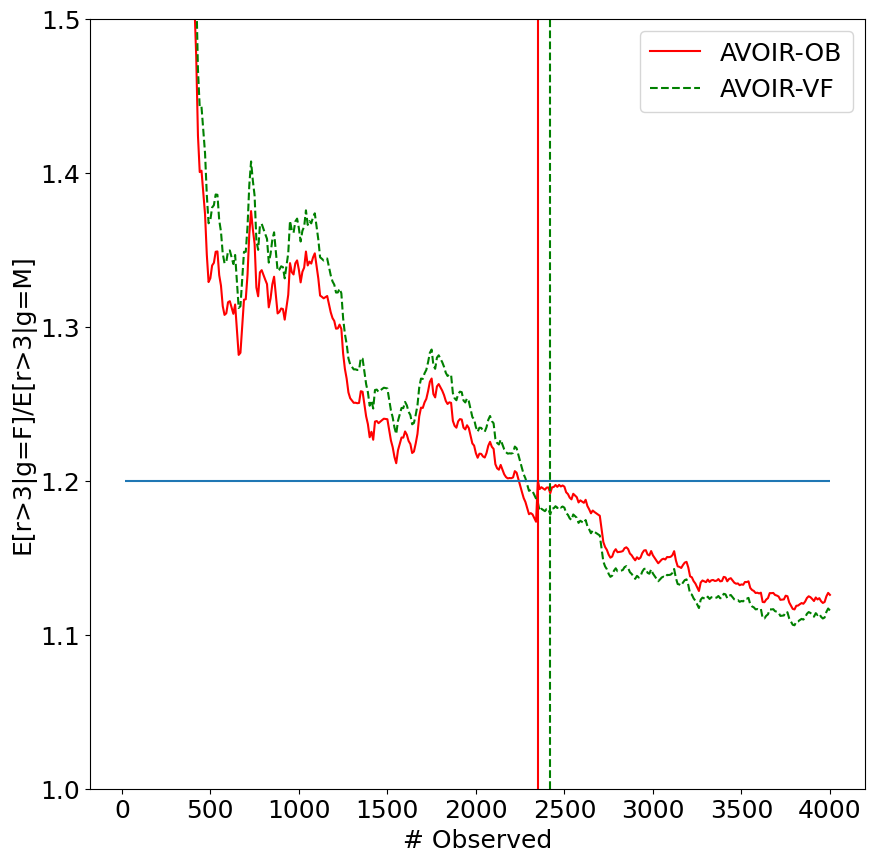
\includegraphics[width=0.5\linewidth]{avoir/images/ratemyprofs.png}
    \caption{Bounds for first half of a gender-fairness specification generated by \AVOIRmethodname{}-OB and \AVOIRmethodname{}-VF for \textit{RateMyProfs}, a real-world dataset. Vertical lines show the step at which the methods can provide a guarantee of failure for the upper bounds with $\Delta <= 0.05$. Blue horizontal line represents the constant term in the inequality.}
    \label{fig:casestudy:rmp}
\end{figure}
This section provides a detailed black-box machine learning model-based case study on a real-world dataset.
This case study uses the Rate My Professors (RMP) dataset~\cite{keymanesh2021fairness}. 
This dataset includes professor names and reviews for them written by students in their classes, ratings, and certain self-reported attributes of the reviewer.
Ratings are provided on a five-point scale (1-5 stars).
We use the preprocessing described in~\cite{keymanesh2021fairness} to infer the gender attribute for the professors.
This dataset is divided into an 80-20 split (train-test).
We then train a BERT-based transformer model~\cite{devlin2019bert} on the training split.
We use the implementation from the simpletransformers\footnote{https://simpletransformers.ai/} package.
The loss function chosen is the mean-squared error from the true ratings.
On the test set, we track a gender-fairness specification in the model outputs:
\begin{lstlisting}[columns=flexible, language=Python, basicstyle=\small]
(E[r > 3 | gender = F] / E[r > 3 | gender = M < 1.2) & 
(E[r > 3 | gender = M)] / E[r > 3 | gender = F] > 0.8)
\end{lstlisting}
We set the failure probability $\Delta = 0.05$. 
\texttt{OPT} is run after each batch (5 items/batch).
Figure~\ref{fig:casestudy:rmp} shows that \AVOIRmethodname{}-OB\footnote{OB = Optimized Bounds} can provide a guarantee in $\mathbf{2.5\%}$ fewer iterations than \AVOIRmethodname{}-VF. 
Note also that the OB guarantee provided tries to optimize for the failure probability while staying under the required threshold, remaining closer to the required threshold in subsequent steps.

\subsection{Adult Income}
\label{sec:casestudy:adult}
In this case study, we analyze the Adult income dataset~\citep{kohavi1996scaling}.
The historical dataset labels individuals from the 1994 census as having a \emph{high-income} ($>50$k a year) or not ($\leq50$k a year).
We consider this column of data as a black-box measurement. 
US Federal laws mandate against race and sex-based discrimination.
Thus, the specification we start our analysis with is a group fairness property for federal employees that monitors the difference of the proportions of individuals with sex marked male vs. female with a high income should be less than $0.5$.
In addition, we ensure that the difference between individuals with race marked white and non-white should have a difference of less than $0.5$.  
Thus, we use an \textit{intersectional} fairness criterion.
The associated specification is given below, where \texttt{h} is an indicator for whether an individual is \emph{high-income} is the binary classification output of our model:

\begin{lstlisting}[columns=flexible, language=Python, basicstyle=\small]
   (E[h | sex=M] - E[h | sex=F] < 0.5) & \ 
   (E[h | race=W] - E[h | race!=W] < 0.5)
\end{lstlisting}

In this example, we set the failure threshold probability $\Delta = 0.15$
\begin{figure}
    \centering
    \begin{subfigure}{0.48\linewidth}
    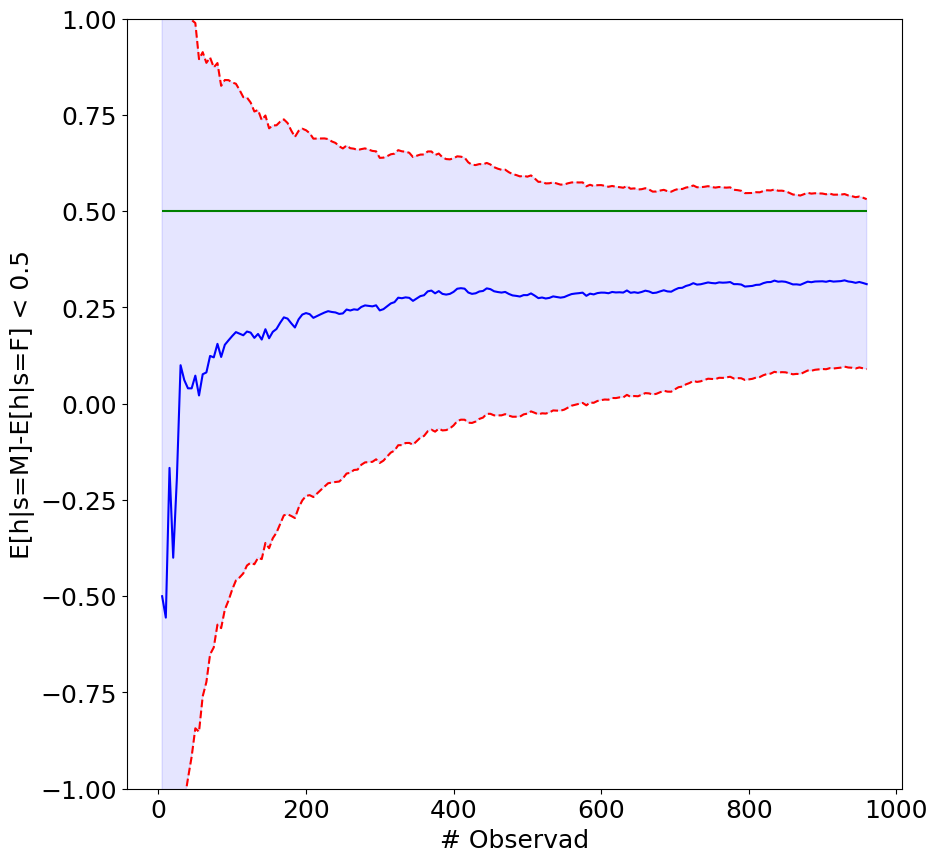
\includegraphics[width=\linewidth]{avoir/images/adult-left-initial.png}
    \caption{Group fairness for sex. Difference in ratio of high income (left subexpression).}
    \label{fig:casestudy:adult:specplot:left}
    \end{subfigure}
    %
    \begin{subfigure}{0.48\linewidth}
    \centering
    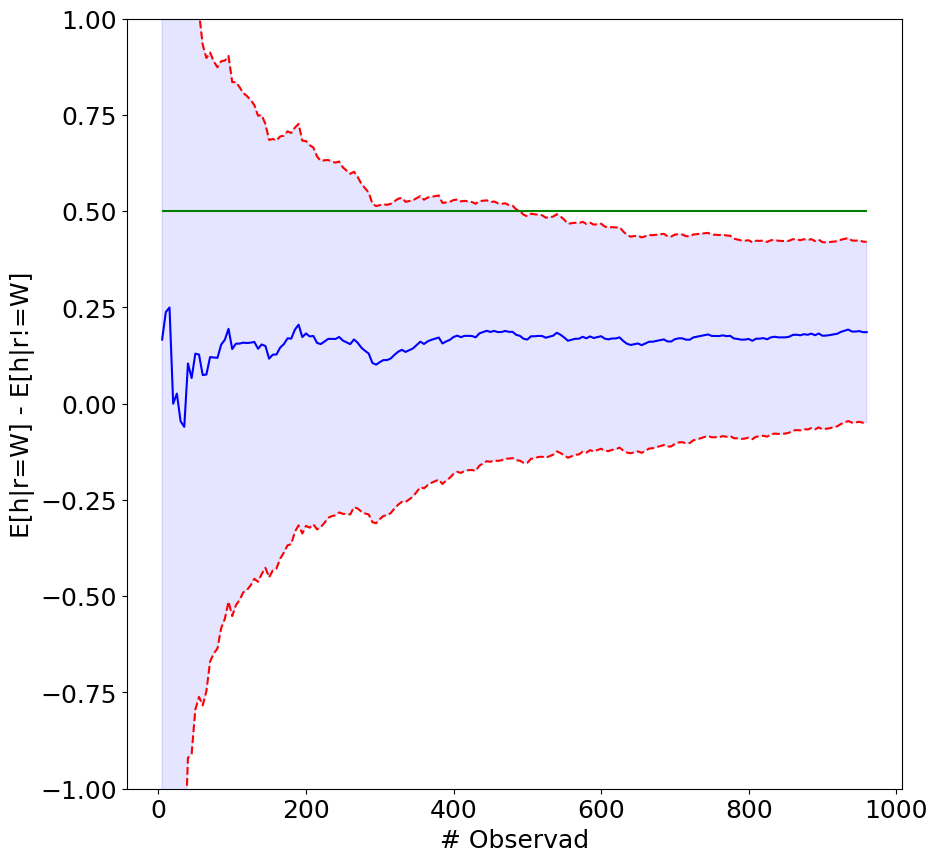
\includegraphics[width=\linewidth]{avoir/images/adult-right-initial.png}
    \caption{Group fairness for race. Difference in ratio of high-income earners (right subexpression). }
    \label{fig:casestudy:adult:specplot:right}
    \end{subfigure}
    \caption{\figtop{} Red dotted lines, the upper bounds of the value cannot be guaranteed to be under the threshold at the specified failure probability. \figbottom{} Guarantee possible with given data. Green lines represent the constant term, and dark blue is the empirical mean.}
\end{figure}
When run with this specification, the generated bounds cannot be achieved with the available data. 
We can then use the iterative refinement associated with subexpressions to analyze different components of the specification. 
The plot corresponding to the left subexpression is shown in Figure~\ref{fig:casestudy:adult:specplot:left} shows that guarantees cannot converge under the threshold with the given number of data samples. 
An auditor can now choose to either reduce the guarantee (i.e. increase $\Delta$) or increase the threshold. 
Next, analyzing the right subexpression, the race group fairness term can be guaranteed to be under the threshold (Figure~\ref{fig:casestudy:adult:specplot:right}).
Using this information, an auditor can make a decision to increase the threshold on the group fairness term for sex. 
As a hypothetical, suppose they increase it from $0.5$ to $0.55$ and rerun the analysis.
OB can provide a guarantee at this threshold within 870 steps, whereas VF can provide it at 960 steps, demonstrating a relative improvement of about $\mathbf{10.35\%}$.
Additionally, the optimal $\Delta$ split across the terms is $\approx (0.135, 0.36 * 10^4)$, which is far from the equal split allocated by VF.
The reason for this split is that increasing the threshold for the first time provides the optimizer with additional legroom to better distribute the failure probabilities between the two terms.

\subsection{COMPAS Risk Assessment}

The Correctional Offender Management Profiling for
Alternative Sanctions (COMPAS) recidivism risk score data is a popular dataset for assessing machine bias of commercial tools used to assess a criminal defendant's likelihood to re-offend.
The data is based on recidivism (re-offending) scores derived from software released by Northpointe and widely used across the United States for making sentencing decisions.
In 2016, \citet{angwin2016machine} at ProPublica released an article and associated analysis code critiquing machine bias associated with race present in the COMPAS risk scores for a set of arrested individuals in Broward County, Florida, over two years.
The analysis concluded that there were significant differences in the risk assessments of African-American and Caucasian individuals.
Northpointe pushed back in a report~\citep{dieterich2016compas} firmly rejecting the claims made by the ProPublica article; instead, they claimed that \citet{angwin2016machine} made several statistical and technical errors in the report.
In this case study, we use \AVOIRmethodname{} to study the claims of the two reports mentioned above. 
%First, we start with the data released by ProPublica and load it into a pandas-simulated DB.
We create a materialized view of the ProPublica dataset by reproducing the preprocessing steps in the publicly available ProPublica analysis  notebook\footnote{https://github.com/propublica/compas-analysis}.
We look at ``Sample A''~\citep{dieterich2016compas}, where the analysis of the ``not low'' risk assessments using a logistic regression model reveals a high coefficient associated with the factor associated with race being African-American.
In terms of a fairness metric, this corresponds to false positive rate (FPR) balance (predictive equality)~\citep{verma2018fairness} metrics. 
The associated specification in \AVOIRmethodname{} grammar would be

\begin{lstlisting}[columns=flexible, language=Python, basicstyle=\small]
   E[hrisk | race=African-American & recid=0] / 
   E[hrisk | race=Caucasian & recid=0] < 1.1
\end{lstlisting}

Where \verb|hrisk| is an indicator for high-risk assessments made by the \emph{black-box} COMPAS tool as defined by ~\citet{angwin2016machine},  \verb|recid| is an indicator for re-offending within two years of first arrest, and a $90\%$-rule is used as the threshold. 
We choose a failure threshold probability of $\Delta = 0.1$, with the optimization run after every batch of $5$ samples.
\AVOIRmethodname{} finds that when the decisions are made sequentially, online, the assertion for specification violation cannot be made with the required failure guarantee.

By analyzing the component subexpressions, one can glean that \AVOIRmethodname{} cannot optimize since the lower FPR in the denominator (FPR for Caucasian individuals) increases the overall variance and limits the ability to optimize for guarantees. 
We follow this analysis by using the reciprocal specification, i.e.,
\begin{lstlisting}[columns=flexible, language=Python, basicstyle=\small]
   E[hrisk | race=Caucasian & recid=0] /
   E[hrisk | race=African-American & recid=0] > 0.9
\end{lstlisting}

We find that the specification is guaranteed to be violated with a confidence of over $1 - \Delta = 0.9$ probability, and \AVOIRmethodname{} can detect this violation within about half the number of available assessments (3350 steps) when run in an online setting.
Figure~\ref{fig:casestudy:compas:propublica} demonstrates the progression of the tracked expectation term. 
Thus, if deployed with the corrected specification, \AVOIRmethodname{} would be able to alert Northpointe/an auditor of a violation/potentially-biased decision-making tool.

\begin{figure}
    \begin{subfigure}{0.48\linewidth}
        \centering
        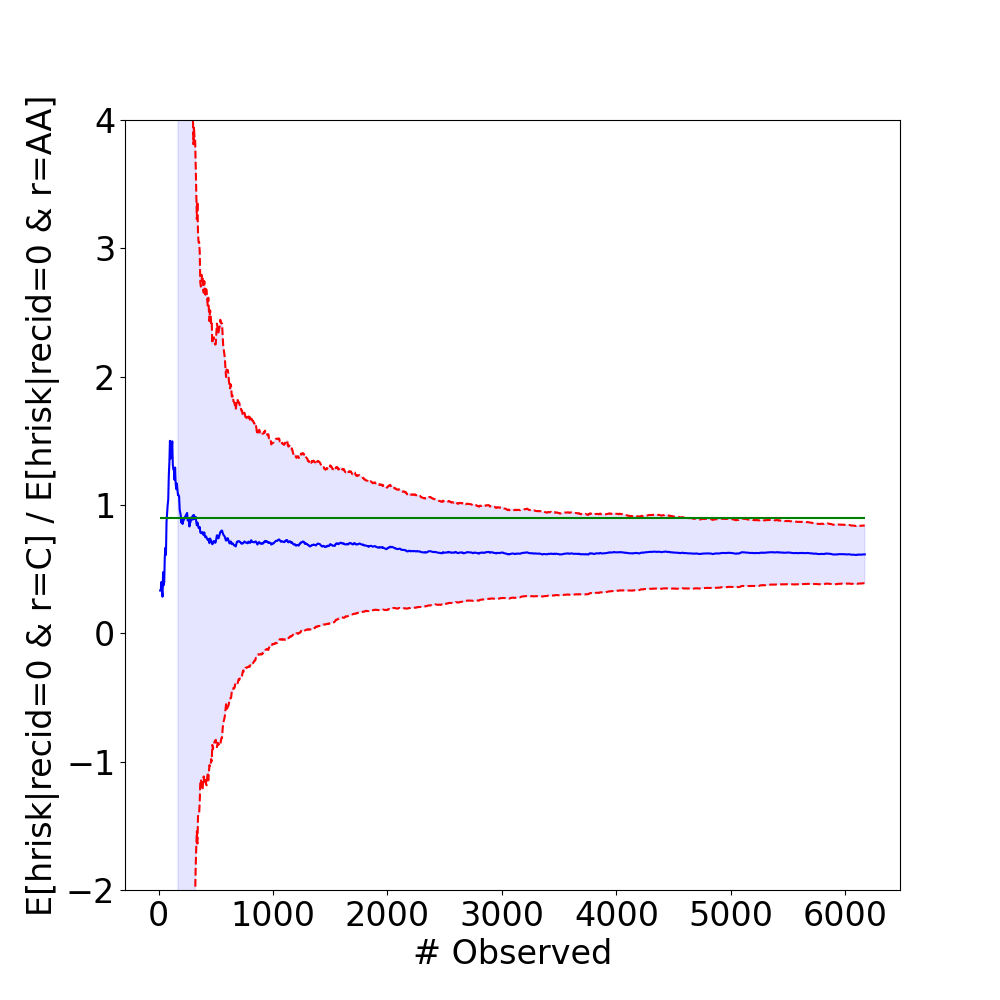
\includegraphics[width=\linewidth]{avoir/images/compas-propublica-et.png}
        \caption{(ProPublica) COMPAS, ``Sample A'' False Positive Rate Bias specification required to \emph{above} the $10\% \implies 0.9$ threshold converges to a value that can be guaranteed to be \emph{under} the required threshold.}
        \label{fig:casestudy:compas:propublica}
    \end{subfigure}
    \hfill
    \begin{subfigure}{0.48\linewidth}
        \centering
        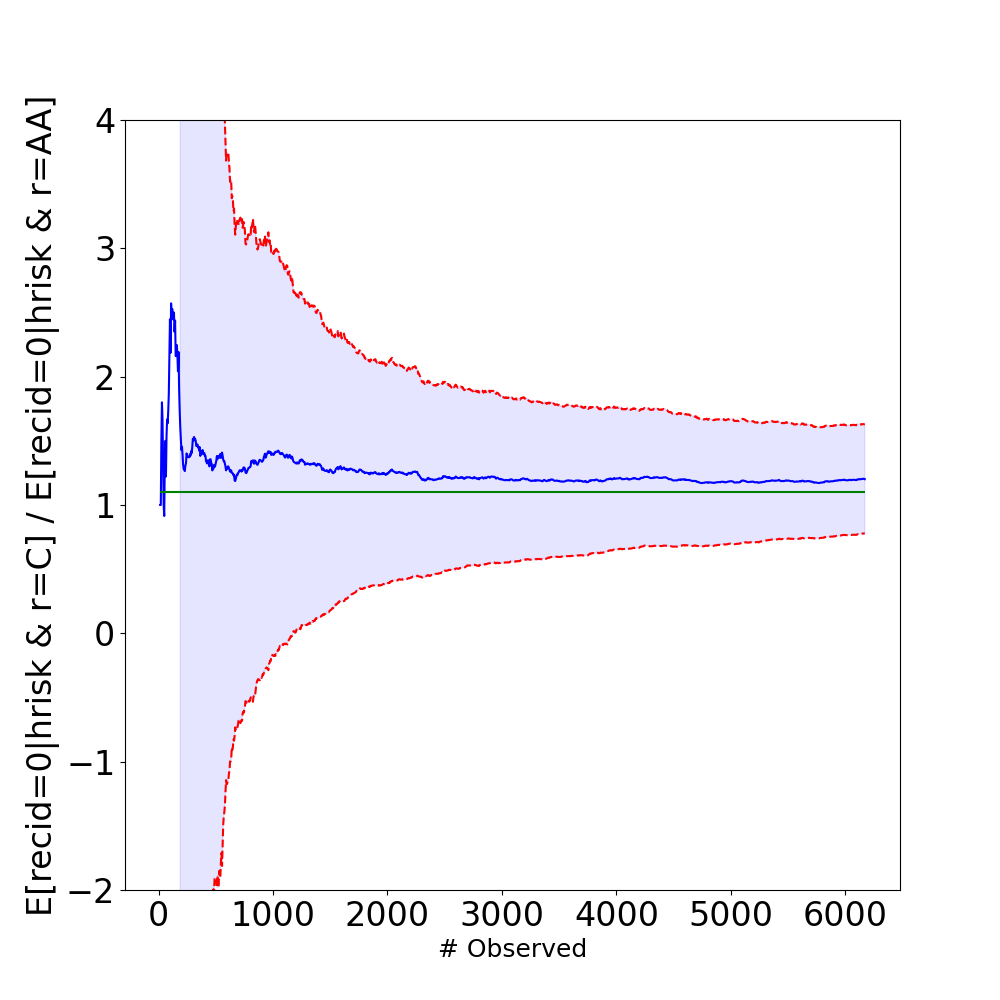
\includegraphics[width=\linewidth]{avoir/images/compas-northpointe-et.png}
        \caption{(Northpointe) ``Sample B'' analysis done by Northpointe using False Discovery Rate that opposed the ProPublica reports.}
        \label{fig:casestudy:compas:northpointe}
    \end{subfigure}
    \caption{COMPAS dataset case study.}
\end{figure}


The Northpointe report~\citep{dieterich2016compas} makes several claims about the shortcomings of this analysis.
One of the primary claims is that \citet{angwin2016machine} used an analysis based on ``Model Errors'' rather than ``Target Population Errors''.
In fairness specification terms, this refers to the difference between a False Positive Rate (FPR) balance vs. False Discovery Rate (FDR) balance, i.e., balancing for predictive parity over predictive equality. 
In probabilistic terms, the difference amounts to comparing $\Pr[\hat{Y} = 1 | Y = 0, g=1, 2]$ (FPR) vs $\Pr[Y = 0 | \hat{Y} = 1, g=1, 2]$ (FDR), where $\hat{Y}$ refers to the decision made by the algorithm, $Y$ refers to the true value, and $g = 1, 2$ reflects group membership~\citep{verma2018fairness}.
This analysis is run on the dataset subset dubbed ``Sample B''.
To test their hypothesis, we reproduce the corresponding preprocessing steps and run both versions (numerator and denominator being Caucasian) of the corresponding specification under the same setup as earlier. 
Despite the point estimate being within the required threshold, we find that neither version can be guaranteed with the required confidence in the given data.
Due to the paucity of space, we describe only one of the two variants with the corresponding figure (Figure~\ref{fig:casestudy:compas:northpointe}).
\begin{lstlisting}[columns=flexible, language=Python]
   E[recid=0 | race=Caucasian & hrisk] /
   E[recid=0 | race=African-American & hrisk] > 0.9
\end{lstlisting}


We note that the Northpointe report~\citep{dieterich2016compas} does not provide confidence intervals for their claim. 
Further, even though the report does not release associated code, the point estimates of the False Discovery Rates (FDRs) match those present in the report, which increases our confidence in our \AVOIRmethodname{}-based analysis. 

The back-and-forth exchange has been the subject of much discussion in academic and journalistic publications~\citep{feller2016computer, washington2018argue}.
Seminal work by \citet{kleinberg2017inherent} proved the impossibility of simultaneously guaranteeing certain combinations of fairness metrics.
While \AVOIRmethodname{} cannot circumvent this problem, its usage can help audit claimed guarantees on defined metrics.
We conclude this case study by noting that \AVOIRmethodname{} lends itself to successful analysis that is not possible with the VF implementation available online, which only provides support for a predefined set of specifications and requires access to a data-generating function.
In addition, we choose $0.1$ as the failure probability because it is one of the thresholds used in \cite{angwin2016machine}.  
We set it to the highest used threshold to allow leeway for the claim by Northpointe.
Even under this lax threshold, the analysis by Northpointe fails.

\section{Discussion} %\& Future Work}
The case studies presented in the previous section demonstrate the ability of our tools to provide vital context when deciding how to refine a model or fairness specification.
Although this contextual information makes decisions easier, it is not always clear how one should alter a specification in light of a violation and its relevant context.
%For example, in case study B, the decision was made that the threshold could be lowered from 2. However, it is not obvious how much we should lower this threshold. Further complicating the matter is the fact that we have options when changing the specification. We can lower the threshold constant (2), or we can add a constant multiplier to the expectation of females with high income.
To assist in these decisions, we are currently examining ways work to suggest edits that are likely to achieve the desired intent of a developer.
Using our visual analysis tool for refinement, we can gather edits from developers and then use that data to learn iterative changes to the syntax tree of the specification.
In addition to improving the usability of our tools for making fairness specification refinements, we also envision a more scalable framework.
Our case studies look at a single model with respect to a single dataset. However, real-world deployment of machine learning often contain many clients with models that may differ.
However, real-world deployment of machine learning often contain many clients with models and datasets that may evolve and drift over time.
We take it as future work to study the efficient monitoring of machine learning behavior with respect to a fairness specification in a distributed context, enabling horizontal scalability.
We believe techniques such as decoupling the observation of data and the reporting results from the monitoring of the results are promising and can lead to the desired scalability.

%\vspace{-0.2in}
\section{Conclusion}

We presented the \AVOIRmethodname{} framework to easily define and monitor fairness specifications online and aid in the refinement of specifications. \AVOIRmethodname{} is easy to integrate within modern database systems but can also serve as a standalone system evaluating whether black-box machine learning models meet specific fairness criteria on specific datasets (including both structured and unstructured data) as described in our case studies.
\AVOIRmethodname{} extends the grammar from Fairness Aware Programming~\cite{albarghouthi2019fairness} with operations that enhance expressiveness.
In addition, we derive probabilistic guarantees that improve the confidence with which specification violations are reported.
Through case studies, we demonstrate that \AVOIRmethodname{} can provide users with insights and context that contribute directly to refinement decisions.
To understand the robustness of \AVOIRmethodname{}, we evaluated it along two dimensions: the data/ML model used and changing parameters (thresholds, fairness definitions).
We demonstrated the robustness of the data/model used by evaluating three datasets of varying domains and types (criminal justice - COMPAS, text classification - RateMyProfs, census data - Adult Income). 
For robustness to the thresholds, we used varying failure probability levels ($0.05$, $0.1$, $0.15$) in our case studies.
Note that any probability thresholds over these values for the corresponding studies would converge in fewer iterations, while lower thresholds would require additional data samples.
Our framework builds the foundation for further improvements in fairness specification, auditing, and verification workflows.
Although contextual information from \AVOIRmethodname{} makes decisions more straightforward, it is not always clear how to alter a specification in light of a violation and its relevant context.

To assist in these decisions, we are currently examining mechanisms that suggest edits that are likely to achieve the desired intent of a model developer.
We plan to extend this work to provide intelligent specification refinement suggestions and support distributed machine learning settings.
In addition to improving the usability of our tools for making fairness specification refinements, we also envision a more scalable framework.
Our case studies looked at a single model with respect to a single dataset. 
However, real-world deployment of machine learning often contains many clients with models and datasets that may evolve and drift over time.
We also expect to examine efficient monitoring of machine learning behavior for a fairness specification in a distributed context, enabling horizontal scalability.
We believe techniques such as decoupling the observation of data and reporting results from monitoring the results are promising and can lead to the desired scalability.
%We also plan to explore the use of \AVOIRmethodname{} for fair ranking problems and tailored database integration.

\newpage \section{Reproducibility}
\label{sec:reproducibility}
To enhance the reproducibility of our work, on the theoretical side, all proofs (with the necessary assumptions) are provided in the appendix. 
Specifically, proofs for the inference engine are in Appendix~\ref{sec:appendix:inference-rules}, and proofs for the correctness of bounds are provided in Appendix~\ref{sec:appendix:confseq}. 
Theorem~\ref{theorem:better-stopping}, which shows how \AVOIRmethodname{} improves over prior work is proved in Appendix~\ref{sec:appendix:optimality}.
To reproduce the results of the case studies in the paper, each case study is encapsulated inside a Jupyter notebook. 
These notebooks are attached along with the source code for \AVOIRmethodname{}.
In addition, all datasets used for generating results for the case studies are also attached in the submitted supplementary documentation.
Finally, the model weights used for the \textit{RateMyProfs} study for exact reproduction are provided in a dropbox folder hosted at  \url{https://www.dropbox.com/sh/n5o4vswnkxv34zr/AABthgLMaYL3MuA0KC39Z1G8a?dl=0}.
\begin{comment}
It is important that the work published in ICLR is reproducible. Authors are strongly encouraged to include a paragraph-long Reproducibility Statement at the end of the main text (before references) to discuss the efforts that have been made to ensure reproducibility. This paragraph should not itself describe details needed for reproducing the results, but rather reference the parts of the main paper, appendix, and supplemental materials that will help with reproducibility. For example, for novel models or algorithms, a link to a anonymous downloadable source code can be submitted as supplementary materials; for theoretical results, clear explanations of any assumptions and a complete proof of the claims can be included in the appendix; for any datasets used in the experiments, a complete description of the data processing steps can be provided in the supplementary materials. Each of the above are examples of things that can be referenced in the reproducibility statement. This optional reproducibility statement will not count toward the page limit, but should not be more than 1 page.
\end{comment}
\begin{subappendices}
\section{Inference Rules}
\label{sec:appendix:inference-rules}
In Figure~\ref{fig:inference}, we provide the rules used to determining the constraints and guarantees for a specification.
We represent $ 
X \odot Y : (E, \epsilon, \delta) \equiv \Pr\left(| \E[X] \odot \E[Y] - E | \geq \epsilon \right) \leq \delta
$
where $\odot$ represents a binary operator.
Constraints are represented in $\{ \}$.
%\pmcomment{Need to explain that constraints carry over in missing cases in Figure!\ref{fig:inference}}
%\pmcomment{Add proofs here for inference rules.}
The proof of correctness for each inference rule starts from the assumptions above the horizontal line and derives the assertions below. 
These proofs use ideas similar to those in \cite{bastani2019probabilistic}.
We reproduce the proofs in Appendix~\ref{sec:appendix:constraint:proofs} here for completeness.
%We provide them here for completeness.
Note that the assertions in the base case (elementary subexpressions) can be arrived at by applying $\rm{AIN}$. 

\begin{figure}
\[
\dfrac{X: \left(\BarE[X], \epsilon_X, \delta_X\right), Y: \left(\BarE[Y], \epsilon_Y, \delta_Y\right)}{X \pm Y: \left(\BarE[X] \pm \BarE[Y], \epsilon_X + \epsilon_Y, \delta_X + \delta_Y\right)}
\]
\[
\dfrac{X: \left(\BarE[X], \epsilon_X, \delta_X\right), Y: \left(\BarE[Y], \epsilon_Y, \delta_Y\right)}{ X \times Y: (\BarE[X] \BarE[Y], \epsilon_X \epsilon_Y + \BarE[X] \epsilon_Y + \BarE[Y] \epsilon_X, \delta_X + \delta_Y)} 
\]
\[
\dfrac{X: \left(\BarE, \epsilon, \delta \right), \BarE - \epsilon > 0}{ X^{-1}: \left(\BarE^{-1}, \frac{\epsilon}{\BarE (\BarE - \epsilon)}  , \delta \right)}\text{ (Inverse)} 
\] 
\[
\dfrac{X: \left(\BarE, \epsilon, \delta \right)}{ X^{-1}: \left(\BarE^{-1}, \frac{\epsilon}{\BarE (\BarE - \epsilon)}  , \delta \right), \{ \BarE - \epsilon > 0\}} \text{ (Inverse C)}
\]
\[
\dfrac{X: \left(\BarE, \epsilon, \delta\right), \BarE - \epsilon > c}{ X > c: (T, \delta)} \text{ (True)} \hspace{0.1in} \dfrac{X: \left(\BarE, \epsilon, \delta \right), \BarE  + \epsilon < c}{ X < c: (F, \delta)} \text{ (False)} 
\] 
\[
\dfrac{X: \left(\BarE, \epsilon, \delta\right)}{ X > c: (T, \delta), \{\BarE - \epsilon > c\}} \text{ (True C)} \]
\[
\dfrac{X: \left(\BarE, \epsilon, \delta \right)}{ X < c: (T, \delta), \{\BarE + \epsilon < c\}} \text{ (False C)} 
\] 
\[
\dfrac{\psi_1: (\B_1, \delta_1), \psi_2: (\B_2, \delta_2)}{\psi_1 \wedge \psi_2: (\B_1 \wedge \B_2, \delta_1 + \delta_2)} \text{ (and)} \hspace{0.01in} \dfrac{\psi_1: (\B_1, \delta_1), \psi_2: (\B_2, \delta_2)}{\psi_1 \vee \psi_2: (\B_1 \vee \B_2, \delta_1 + \delta_2)} \text{ (or)}
\]
\[
\dfrac{\psi_1: (\B_1, \delta_1), \{C_{11, \dots, 1k}\}, \psi_2: (\B_2, \delta_2), \{C_{21, \dots, 2m}\}}{\psi_1 \wedge \psi_2: (\B_1 \wedge \B_2, \delta_1 + \delta_2), \{C_{11, \dots, 1k}, C_{21, \dots, 2m}\}} \text{ (and C)} \]
\[
\hspace{0.2in} \dfrac{\psi_1: (\B_1, \delta_1), \{C_{11, \dots, 1k}\}, \psi_2: (\B_2, \delta_2)}{\psi_1 \vee \psi_2: (\B_1 \vee \B_2, \delta_1 + \delta_2),  \{C_{11, \dots, 1k}\} \vee \{C_{21, \dots, 2m}\}} \text{ (or C)}
\]%
\caption{Inference rules used to guarantees for expressions.The inference rules for each compound expression build on the union bound, triangle inequality, and structural induction approach described by \citet{bastani2019probabilistic}. C: Constraint.}
\label{fig:inference}
\end{figure}
\subsection{Inference rules with Constraints}
\label{sec:appendix:constraint:proofs}

%We define guarantees for concentration using an appropriate concentration inequality. 
%Examples are provided in the Appendix~\ref{sec:appendix:inequality}  
%\paragraph{Correctness} 
In Section~\ref{sec:theoretical:propagation} we provided the proofs for $X\pm Y$, $X > c$.
In the following text, we provide the remaining proofs.

\noindent \textit{Product} Starting with $\phi_X, \phi_Y$
%$\phi_X \eqdef (\BarE[X], \epsilon_X, \delta_X)$, $\phi_Y = Y: (\BarE[Y], \epsilon_Y, \delta_Y)$. 
First, from union bound, both of these hold true with probability at least $1 - \delta_X - \delta_Y$.
Then,
{\allowdisplaybreaks
\begin{align*}
|\E[X]| &= |\BarE[X] - \BarE[X] + \E[X]|\\
        &\leq ||\BarE[X]| +  |\BarE[X] + \E[X]| \leq ||\BarE[X]| + \epsilon_X \\
\end{align*}
}
%We have
\begin{align*}
    |\BarE[X]\BarE[Y] &- \E[XY]|  = |\BarE[X]\BarE[Y]  - \E[X]\E[Y]| \\
    %&= |\BarE[X]\BarE[Y] - \BarE[X]\E[Y] + \BarE[X]\E[Y]  - \E[X]\E[Y]| \\
    &= |\BarE[X](\BarE[Y] - \E[Y]) + \E[Y] (\BarE[X]\  - \E[X])| \\
    &\leq |\BarE[X]||(\BarE[Y] - \E[Y])| + |\E[Y]||(\BarE[X]\  - \E[X])| \\
    &\leq |\BarE[X]| \eps_Y + |\E[Y]| \eps_X \\
    &\leq |\BarE[X]| \eps_Y + (|\BarE[Y]| + \eps_Y) \eps_X \\
    &= |\BarE[X]| \eps_Y + |\BarE[Y]| \eps_X + \eps_X \eps_Y
\end{align*}
where the first step follows as $X, Y$ are Bernoulli r.vs.
Therefore, $X \times Y: (\BarE[X] \BarE[Y], \epsilon_X \epsilon_Y + \BarE[X] \epsilon_Y + \BarE[Y] \epsilon_X, \delta_X + \delta_Y)$

\textit{Inverse/Inverse C} Assume $X: \left(\BarE, \epsilon, \delta \right)$ and $\BarE - \epsilon > 0$.
In the constrained case, we start with only the prior assumption. % i.e., $X: \left(\BarE, \epsilon, \delta \right)$
Then,
\begin{align*}
    |\E[X]| &= |\E[X] - \BarE[X] + \BarE[X]| \\
    &\leq |\E[X] - \BarE[X]| + |\BarE[X]| \leq \epsilon_X + |\BarE[X]|
\end{align*}
i.e., $|\E[X]| \leq \epsilon_X + |\BarE[X]|$. 
Also,
\begin{align*}
    |\E[X]^{-1} - \BarE[X]^{-1}| &= \left|\frac{\BarE[X]^{-1} - \E[X]^{-1}}{\BarE[X]  \E[X]^{-1}}\right| \\
    &\leq \frac{\epsilon}{|\E[X]|  |\BarE[X]|} \leq \frac{\epsilon}{|\E[X]| (\E[X] - \epsilon_X)}
\end{align*}
%where the last step follows from the previous derivation and if $\E[X] - \epsilon_X > 0$.
%The latter condition enforces that the sign of the inequality does not change.
VF adds $E[X] - \epsilon_X > 0$ as a precondition; \AVOIRmethodname{} as a post-constraint.
\paragraph{Boolean Operators}
Starting from $\psi_1: (b_1, \delta_1)$, $\psi_2: (b_2, \delta_2)$, we can apply the union bound for $\psi_1 \wedge \psi_2$, $\psi_1 \vee \psi_2$ to derive the rules for and/or.
%\pmcomment{TODO: Complete Proofs}
Similarly, constraints follow the semantics specified by the rules as they also follow from the union bound.




\subsection{Inferred Optimization Problem}
\label{sec:appendix:inferrence-rules:opt}
For a given overall specification $\psi$, suppose $(\epsilon_i, \delta_i$), $i \in \{1, \dots, n\}$ represents the concentration bounds associated with each constituent elementary subexpression. 
Using the inference rules, we can derive the overall $\delta_T = \sum\limits_{i}\delta_i$, along with a set of (say) $K$ constraints 
\[
g_k(\epsilon_{1}, \dots, \epsilon_{n}, \BarE[X_1], \dots, \BarE[X_n]) \leq \epsilon_k
\]
\[
\text{where } \epsilon_k = \left|c_k - \BarE[f(\BarE[X_1], \dots, \BarE[X_n])]\right|
\]
denotes the maximum allowed margin for the $\text{k}^{\text{th}}$ subexpression of form \texttt{<ETerm> <comp-op> c}).
The objective is to minimize the overall failure probability $\delta_T$.
The overall optimization problem can then be formulated as shown in \ref{eq:optimization},
having $n$ optimization variables $\delta_i$ and $2n + K$ constraints (bounds on $\delta_i$ provide the $2n$ constraints).  
A developer using \AVOIRmethodname{} inputs a required acceptable upper bound of failure probability $\Delta$.
If the solution to the optimization problem $\delta_T^* = \sum_i \delta_i \leq \Delta$, then the optimization can conclude with the required confidence in the proved guarantee.
At this point, the developer may choose to terminate \AVOIRmethodname{}.
However, using Corollary~\ref{thm:adaptive-stopping:anytime}, they may continue to run and refine the estimates.

% Metrics table


\section{Concentration bounds}
%Recall the adaptive Hoeffding inequality~\citep{zhao2016adaptive, bastani2019probabilistic} from \Cref{thm:adaptive-stopping}. 

%\AIN*
%\newtheorem{theorem}{Theorem} % TODO: move to my_definitions.tex


Theorem~\ref{thm:adaptive-stopping} provides a mechanism for choosing the stopping time using arbitrary methods for a fixed $\delta$. 
In general, any adaptive concentration inequality suffices; we use $\rm{AIN}_H$ %that does not depend on the empirical variance but is frequently used in scenarios dealing with bounded r.vs.
However, we use confidence intervals to visualize the evolution of sub-expressions (and overall specification) over the sequence of observations. 
To do so, we require an additional result.

\begin{theorem}\cite[Proposition 1, Lemma 1]{zhao2016adaptive}
Let $S_n = \sum_{i=1}^n X_i$ be a random walk from i.i.d. random variables $X_1, \dots, X_t \sim D$. For any $\delta > 0$,
$\Pr[S_\gT \geq f(\gT)] \leq \delta$
for any stopping time $\gT$ if and only if
$\Pr\left[\exists n, S_t \geq f(t) \right] \leq \delta$

\label{thm:zhao:adaptive-hoeffding:anytime}
\end{theorem}

\begin{corollary}
\label{thm:adaptive-stopping:anytime}
For $\delta > 0$, $\Pr[|\BarE_\gT[X] - \E[X]| \leq \epsilon(\delta, \gT)|] \geq 1 - \delta $
for any stopping time $\gT$ if and only if
\[
\Pr\left[\forall t, |\BarE_t[X] - \E[X]| \leq \epsilon(\delta, t)| \right] \geq 1 - \delta
\]
\end{corollary}
%\begin{proof}
%\pmcomment{need to correct this} 
Corollary~\ref{thm:zhao:adaptive-hoeffding:anytime} follows directly from applying Theorem~\ref{thm:zhao:adaptive-hoeffding:anytime} to Theorem~\ref{thm:adaptive-stopping}.
%\end{proof}
Intuitively, Theorem~\ref{thm:adaptive-stopping} holds since we can choose an adversarial stopping rule for $\gT$ that terminates as soon as the boundary for $\epsilon(\delta, t)$ is crossed~\citep{zhao2016adaptive}. 
Thus, when we establish a bound with a stopping rule, %, as long as the underlying distribution remains unchanged,
the bound will hold prior to and after the stopping rule is enforced.
Corollary~\ref{thm:adaptive-stopping:anytime} implies that once we choose an optimal bound for each subexpression, we can extend the bounds derived using Theorem~\ref{thm:adaptive-stopping} to following observations with continued guarantees for subexpressions.
%Note that this does not necessarily imply that the specification will still be True/False with a bounded failure probability since the truth value of the specification depends on the empirical mean.

\subsection{Proof of Theorem~\ref{thm:conf-seq} for Specifications}
\label{sec:thm:conf-seq:proof:contd}

%Recall \Cref{thm:conf-seq}
%\confseq*

Consider any specification $\psi_k$. Let $\psi_k^t : (\hat{b}_{\psi_k}(t), \delta_{\psi_k}(t))$,
where $\hat{b}_{\psi_k}(t) \subseteq \{T, F\}$ is the inferred value and $\delta_{\psi_k}(t)$ corresponds to the confidence for the assertion at time $t$. 
Let the \textit{elementary} subexpressions involved be $X_{k_1}, \dots, X_{k_D}$ corresponding to the index multiset $\etB_k = \{\{k_1, \dots, k_D \}\}$.
Denote $b_{\psi_k}$ as the true value of $\psi_k$, and $\delta_{\psi_k}$ as the inferred threshold at stopping time $\gT$.
From $\rm{INFER}$, we have
\begin{equation}
\hat{b}_k(t), \delta_{\psi_k}(t) = \rm{INFER}(\phi^t_{X_{k_1}}, \dots, \phi^t_{X_{k_D}})
\label{eqn:conf-seq:compound:inf2}
\end{equation}
\begin{align*}
     \Pr[&\exists t \geq 1, b_k \not\in \hat{b}_k(T)]\\
        &\leq \Pr\left[\bigcup\limits_{i = 1}^{D} \exists t \geq 1,  \neg \phi_{X_{k_i}}^t \right]  & \text{ (From \ref{eqn:conf-seq:compound:inf2})} \\
      &\leq \sum\limits_{i\in \etB_k}\Pr\left[\exists t \geq 1, \neg \phi^t_{X_{k_i}}\right]  & \text{ (union bound)} \\
      &= \sum\limits_{i\in \etB_j}\Pr\left[\exists t \geq 1, |\BarE_t[X_{k_i}] - \E_t[X_{k_i}| > \epsilon_{X_{k_i}}(t)\right]  \\
      %& \text{(definition of $\phi^t_{X_{k_i}}$ )} \\
      &\leq \sum\limits_{i\in \etB_j} \delta_{X_{k_i}} & \text{(elementary subexpressions)} \\
      &\leq \delta_{\psi_k}  & \text{ (applying \ref{eqn:conf-seq:compound:inf1} for $t = \gT$)}
\end{align*}
Thus, $b_{\psi_k}(t)$ is a $1-\delta_{\psi_k}$ confidence sequence for $b_{\psi_k}$



\section{Termination Criterion for \AVOIRmethodname{}}
\label{sec:appendix:optimality}
%\betterstopping*
\addtocounter{theorem}{-1}
\begin{corollary}
Under mild conditions, \AVOIRmethodname{} terminates in finite steps with an assertion over the required specification.
\label{corollary:termination}
\end{corollary}
\begin{proof}
We know that the stopping time $\gT \leq \gT^+$, the stopping time for \AVOIRmethodname{}.
Thus, \AVOIRmethodname{} would terminate whenever Verifiar can. 
For completeness, we provide the conditions under which Verifair terminates.
Note that $c \in \R$ corresponds to a constant threshold involved in specification, also presented in the grammar and bound proagation rules.
\begin{itemize}
    \item  For every subexpression $C_k$ occurring in the specification such that it is involved in the inverse or inverse constr. rules (i.e., $\BarE[C_k]^{-1}$), $\BarE[C_k] \neq 0$, $C_k \neq 0$
    \item For every subexpression $C_k$ such that it occurs a True/False type inequality (such as $C_k > c$), $\BarE[C_k] \neq c$, $C_k \neq c$
\end{itemize}
\end{proof}


\section{Supported Metrics}
\label{sec:appendix:additional-metrics}
\begin{table}
    \centering
    \small
    \begin{tabular}{lc}
    \toprule
        Metric Name  & Definition/DSL  \\
    \midrule 
      \multirow{2}{*}{Statistical Parity \citep{dwork2012fairness}} & $\Pr[R|S] = \Pr[R|\neg S]$ \\ 
      \cmidrule{2-2}
      & $\E[r|s] / \E[r|!s] < c$ \\
      \midrule
       \multirow{2}{*}{Predictive Parity \citep{chouldechova2017fair}} & $\Pr[Y|R, S] = \Pr[Y|R, S]$ \\ 
       \cmidrule{2-2}
       & $\E[y|r, s] - \E[y|r, s] > c$ \\
       \midrule
       \multirow{2}{*}{Equal Opportunity \citep{hardt2016equality}} & $\Pr[\neg R|Y, S] = \Pr[\neg R|Y, \neg S]$ \\ 
       \cmidrule{2-2}
       & $\E[!r|y, s] - \E[!r|y,!s] < c$ \\
       \midrule
       \multirow{3}{*}{Equalized Odds \citep{hardt2016equality}} & $\Pr[R|Y=i, S] = \Pr[R]Y=i, \neg S]$, $i=0, 1$ \\ 
       \cmidrule{2-2}
       & $(\E[r|y=0, !s] - \E[r|y=0, s] > c_0)\ \&$ \\
       & $(\E[r|y=1, !s] - \E[r|y=1, s] > c_1)$ \\   
      %  & $ & $(\&  $ \\
       % & $i = 0, 1$ & $(\E[d=1|Y=0, G=f] - \E[d=1|Y=0, G=m] > c_2$\\
    \bottomrule
    \end{tabular}
    \caption{Examples of supported metrics.}
    \label{tab:appendix:supported-metrics}
\end{table}

We provide a non-exhaustive list of statistical group-based fairness criteria and show an exact/approximate equivalent in the \AVOIRmethodname{} DSL in Table~\ref{tab:appendix:supported-metrics}.
We use the notation from Table~\ref{tab:definitions}, assuming that the return value $R$ is a Bernoulli r.v.
We assume that the decision function $f$ tracked by \AVOIRmethodname{} as a signature that takes $X, G, Y$ as input and produces $S$ or $d$ as output.
Note that in their python implementation, $=$ would be replaced by \lstinline{==} and $|$ by the \lstinline{given} keyword.
\begin{comment}
\begin{itemize}
    \item[$G$:] Protected or sensitive attribute. For demonstration purposes, we will use the values $m$ and $f$ to denote majority and minorty classes.
    \item[$X$:] Features describing each individual 
    \item[$Y$:] True label for $X$
    \item[$S$:] Probability $\Pr[Y|X, G]$ predicted for a certain class $c$
    \item[$d$:] Predicted decision for $X$, usually derived from $X$
    \item[$c$:] A threshold to test the specification. For ratios based approximations, this would be a number $1 \pm \eps$ for some small $\eps > 0$. For difference based approxiamtions, this number would be some small $\eps > 0$. When multiple terms are present, we use $c_i$ to denote the $i^{\text{th}}$ threshold.
\end{itemize}
\end{comment}

\section{Implementation Details}
We built a python library to create specifications that can be implemented as a decorator over decision functions. 
The front end interactive application was implemented using streamlit\footnote{https://streamlit.io/} and the visualizations were built in Vega~\cite{satyanarayan2015reactive}.
Each term in the DSL is implemented through a corresponding python class.
New input/output observations are monitored to update all the terms in a specification.
Inference for evaluating the value and bounds is carried out via operator overloading in these classes. 
%This is fairly straightforward.
In line with previous work~\citep{albarghouthi2017fairsquare,bastani2019probabilistic,albarghouthi2019fairness} on distributional verification, we use rejection sampling for conditional probability estimation.
%In the remainder of this section, we describe how how each of these components are implemented. Further, we describe the process for computing point estimates and probabilistic confidence intervals for the values computed for different terms within the spec.



% Typical fairness constraints require 
%Figure~\ref{fig:grammar} describes the final grammar of our specification DSL.

\subsection{Visual Analysis}
\label{sec:implementation:vis}
\begin{figure}
    \centering
    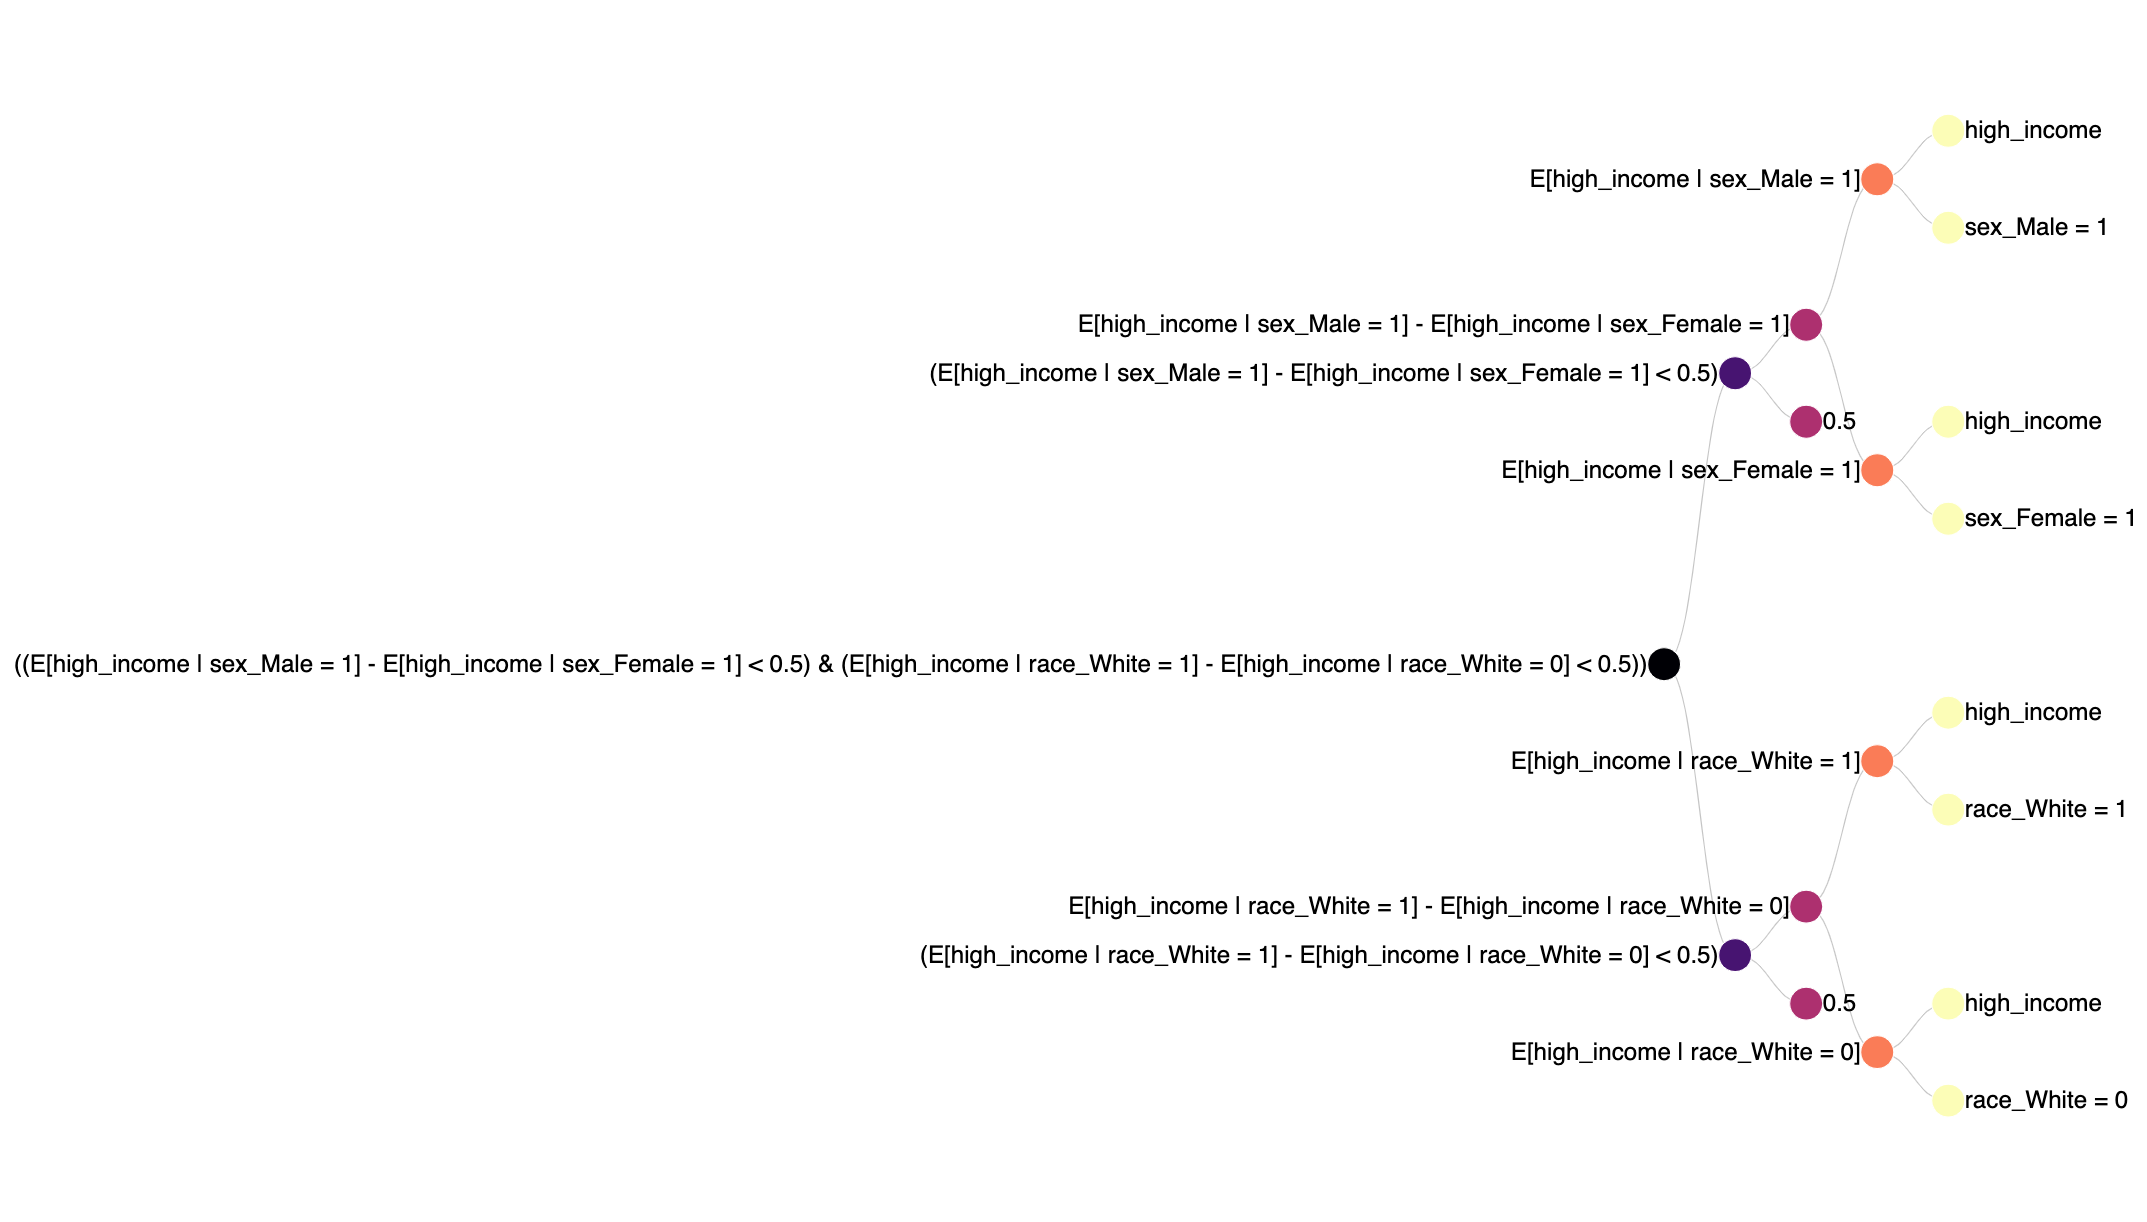
\includegraphics[width=\textwidth, angle=90,alt={Internal representation of parsed tree for a specification.}]{avoir/images/adult-spec-tree-initial.png}
    \caption{Tree corresponding to the initial specification for the Adult Income dataset.}
    \label{fig:impl:adult:initial-spec}
\end{figure}

Using our specification framework as a backend, we built an interactive application for analysis and refinement of specifications provided in our grammar.
Given a user provided machine learning model, dataset, and specification the application simulates a stream of observations to the provided model.
Following the simulation, a visualization is provided that represents the specification as a syntax tree where each node of the tree corresponds to an element of our grammar.
Figure \ref{fig:impl:adult:initial-spec} shows the visualization.

Note that for each observation made by our machine learning model, the specification is evaluated to check for violations.
Each grammar element that makes up the specification is evaluated as well, and thus each grammar element is associated with the value it evaluates to for a given observation.
For specifications \texttt{<spec>}, there is a boolean value associated with each observation, whereas an expectation term, \texttt{<ETerm>}, is associated with a real value.
By selecting one of the nodes in the syntax tree, a user can see a plot of the evaluation values associated with the selected grammar element.
We call these plots evaluation plots and two can be observed at a time 
%(see the plots on the right of figure \ref{fig:casestudy:boston}),
each with shared scales along the horizontal axis which denotes observations over time.
This allows for comparison of multiple grammar elements.
The ability to analyze and compare these evaluation values provides context surrounding specification violations, and assists the user in deciding how to refine a specification.
The case studies in section \ref{sec:casestudy} demonstrate the usefulness of the context provided by these visualizations.

The app for interaction with the backend is built using streamlit. It proceeds in multiple stages,
\begin{enumerate}
    \item First, a user selects a dataset of interest. We built support for four datasets, but our framework is generic enough for any arbitrary csv dataset.
    \item Following this choice, the input variables and output variable for a machine learning model must be specified.
    \item A machine learing model is then selected from a dropdown. We provide support for three models. However, this is for demonstration purposes only - the specification is agnostic to the choice of a machine learning model.
    \item Finally, a specification is input by the user of the app. On the press of a button, the model is trained and then evaluated on the selected dataset. The output monitored by the spec is passed off to the Vega module for further analysis.
\end{enumerate}

\section{AVOIR in Database Setting}

\begin{comment}
\begin{table}
    \centering
    \caption{A summary of the results from the case studies.}
    \label{tab:casestudy:summary}
    \begin{tabular}{ccc}
    \toprule
         Dataset & Setting & Improvement over~\cite{bastani2019probabilistic}  \\
         \midrule
         Adult Income & Database & $10.35\%$ \\
         COMPAS & Materialized View & Interaction\\
         Rate my Profs & ML - BERT & $2.5\%$ \\
         \bottomrule
    \end{tabular}

\end{table}
\end{comment}

In the database literature researchers~\cite{nargesian21tailoring}, have explored an approach to tailoring data integration strategies to ensure that the data set used for analysis has an appropriate representation of relevant (demographic) groups and it meets desired distribution requirements. The authors describe how to acquire such data in an approximate cost-optimal manner for several realistic settings. This work is orthogonal to our work and yet AVOIR can potentially integrate with the authors approach to examine if fairness criteria are being met during the integration process. In other studies on fairness researchers~\cite{yang2018nutritional,asudeh19a,asudeh19b}, have considered the problem of personalized fair ranking functions and discuss approaches to determine if a proposed ranking function satisfies a set of  desired fairness criteria and, if it does not, to suggest modifications that do. AVOIR attempts to solve a  more general purpose problem (not limited to any particular fairness criteria) and is agnostic to the specific model (treats it as a blackbox).  While we have not examined the performance of AVOIR for fair ranking problems, it is something we plan to examine in the future.

To demonstrate how \AVOIRmethodname{} can be integrated within a database system
we use pandas\footnote{https://pandas.pydata.org/} dataframes to simulate the application of \AVOIRmethodname{} in the database setting. 
Specifically, we wrap pandas dataframes with a python `Database' class, and provide a query mechanism to create materialized views.
Queries are provided in the form of python functions that take a dataframe as input and output a corresponding dataframe.
The corresponding view thus generated can be updated with insertion/update/deletion of data.
The specification is added as a decorator inside the refresh function, allowing \AVOIRmethodname{} to track specifications in a database setting.
Note that this tie-in with pandas is only for ease of implementation; the inference engine and optimization can be extended to any database engine.


\end{subappendices}


\endinput

\chapter{Conformal Prediction for Graph Structured Data}
\label{chp:graphConformal}
In the previous chapter, confidence intervals were used to generate online, anytime-valid bounds for the outputs associated with different decision-making models.
However, confidence intervals require a strong assumption on the data-generating distribution at test time i.e, independent and identically distributed (i.i.d) data.
For graph structured data, the edges between different nodes denote potential dependencies between the nodes.
Thus, the i.i.d assumption is violated, and the confidence intervals are no longer valid.
In this chapter, we will discuss conformal prediction, a method that provides valid confidence sets/intervals for graph structured data under a weaker assumption - exchangeability.
While the estimates generated by these are no-longer online, anytime-valid, the strong guarantees provided by these methods can provide a foundation for understanding the uncertainty associated with the predictions in graph structured data.
In this chapter, we will discuss the theoretical underpinnings of conformal prediction and the tradeoffs associated with its application to graph structured data.
%\pmcomment{Maybe move this to appendix}
%Following this, in the second part, we will conclude with a discussion of extending conformal prediction for studying the fairness of decision-making models trained for graph structured data.

%\section{Understanding the Tradeoffs in Graph Conformal Prediction}

Conformal prediction has become increasingly popular as a method for quantifying the uncertainty associated with machine learning models. 
The computational efficiency of the inductive approach has made it the method du jour for building new methods for conformal prediction.
Recent work in graph uncertainty quantification has built upon this approach for conformal prediction on graphs.
The nascent nature of these explorations has lead to conflicting choices for implementations baselines and evaluation of approaches.
We critically analyze the choices made and describe the tradeoffs associated with existing graph conformal prediction work. 
Our theoretical and empirical results provide the rationale for our recommendations for future scholarship in graph conformal prediction.

\section{Introduction}
Modern machine learning models trained on losses based on point predictions are prone to be overconfident in their predictions~\citep{guo2017calibration}. 
The Conformal Prediction (CP) framework~\citep{vovk2005algorithmic} provides a mechanism for generating statistically sound post hoc prediction sets (or intervals, in case of continuous outcomes) with coverage guarantees under mild assumptions.
The usual assumption made in CP is that data are exchangeable, i.e, the joint distribution of the data is invariant to permutations of the data points.
The guarantees provided by CP are distribution-free, and can be added post hoc to arbitrary, black-box predictor scores.
This makes CP an ideal candidate for quantifying uncertainty in complex models, such as neural networks.

Network-structured data such as social networks, transportation networks, and biological networks are ubiquitous in modern data science applications.
Graph Neural Networks (GNNs) have been developed to model vector representations of such network-structured data, and have been shown to be effective in a variety of tasks such as node classification, link prediction, and graph classification~\citep{hamilton2020graph, wu2022graph}.
Uncertainty quantification approaches built for independent and identically distributed (iid) data cannot directly be applied to graph data, as the network structure introduces dependencies between the data points.
However, recent work~\citep{clarkson2023distribution,zargarbashi23conformal,huang2024uncertainty} has demonstrated that in certain settings, CP can be applied to graph data to generate statistically sound prediction sets for the node classification task.

Variations of CP include full CP~\citep{vovk2005algorithmic} which has significant computational cost as the score function must be recomputed with replacement for each data point within the calibration set.
Additionally, cross-conformal prediction~\citep{vovk2015cross}, CV+/Jackknife+~\citep{barber2021predictive} are other variations of CP which are computationally more efficient than full CP, but less efficient than split CP.
Prior work in CP on graphs has mainly focused on the split CP setting due to its computational efficiency, ease of implementation, and distribution-free guarantees with black-box models. 
We focus on split CP in this work.
There is a lack of consensus for the choice and setup of baselines, splitting of common datasets, and evaluation metrics for methods.
In this work, we aim to analyze the choices made by existing work and understand the trade offs associated with these choices.
%In addition, we create a python library which implements different variations of these approaches which would help standardize practices in the evaluation of CP for graph data.


\section{Conformal Prediction}
Conformal prediction is used to quantify the uncertainty of a model by providing prediction sets/intervals with coverage guarantees.
We will focus on conformal prediction in the classification setting.
Given a calibration dataset $\gD_{\text{calib}} = \{(\vx_i, y_i)\}_{i=1}^n$, where $\vx_i \in \gX = \R^d$ and $y_i \in \gY = \{1, \dots, K\}$, conformal prediction can be used to construct a prediction set $C$ such that
\begin{align*}
    \Pr\left[y_{n+1} \in C(\vx_{n+1}) \right] \geq 1 - \alpha
\end{align*}
where $1 - \alpha \in [0, 1]$ is a user-specified coverage level.
The only assumption required for the coverage guarantee is that $\gD_{\text{calib}} \cup \{(\vx_{n+1}, y_{n+1})\}$ is exchangeable.
The following theorem provides a general recipe for constructing a prediction set with coverage guarantee.
\begin{theorem}[\citet{vovk2005algorithmic}]
    Suppose $\{(\vx_i, y_i)\}_{i=1}^{n+1}$ are exchangeable, $s: \gX \times \gY \rightarrow \R$ is a score function, and $\alpha \in [0, 1]$ is a target significance level.
    Let $\hat{q}(\alpha) = \text{Quantile}\left(\frac{\ceil{(n+1)(1-\alpha)}}{n}; \{s(\vx_i, y_i)\}_{i=1}^{n}\right)$
    Define $C_{\alpha}(X) = \{y \in \gY: s(\vx, y) \leq \hat{q}(\alpha)\}$.
    Then,
    \begin{align}
        1 - \alpha +\frac{1}{n+1} \geq \Pr\left[y_{n+1} \in C_{\alpha}(\vx_{n+1}) \right] \geq 1 - \alpha
        \label{eq:CP:coverage}
    \end{align}
    \label{thm:CP:coverage}
\end{theorem}

While Theorem~\ref{thm:CP:coverage} does not place any restrictions on the choice of the score function, the choice of the score function can have a significant impact on the size of the prediction set.
$s$ is usually called the non-conformity score function which measures the degree of non-agreement between the input $\vx$ and the label $y$ i.e., larger scores indicate worse agreement between $\vx$ and $y$.
Note that the setup of theorem~\ref{thm:CP:coverage} is called split CP, which is a special case of CP.
Further, it only provides a marginal coverage guarantee.
\pmcomment{discuss the difference between marginal and conditional coverage and requirements for conditional coverage. Additionally, discuss beta distribution?}



%\section{Applying Conformal Prediction to Graph Structured Data}
\section{Node Classification and Conformal Prediction in Graphs}
The usual tasks of interest in graph data are node classification, link prediction, and graph classification. 
In this work, we focus on node classification and its extensions to conformal prediction.
Consider an attributed homogeneous graph $\gG = (\gV, \gE, \mX)$, where $\gV$ is the set of nodes, $\gE$ is the set of edges and $\mX$ is the set of node attributes.
Let $\mA$ denote the adjacency matrix for the graph.
Further, let $\gY = \{1, \dots, K\}$ denote set of class labels associated with the nodes.
For $v \in \gV$, $\vx_v \in \R^d$ denotes its features and $y_v \in \{1, \dots, K\}$ denotes the corresponding class label.
The task of node classification is to learn a model $F: \gX \to Y$ which predicts the label for each node given node features as input.
Corresponding to the CP partitions, we denote the nodes in the training set as $\gV_{\text{train}}$, validation set as $\gV_{\text{valid}}$, calibration set as $\gV_{\text{calib}}$, and test set as $\gV_{\text{test}}$.
We denote $\gV_d = \gV_{\text{train}} \cup \gV_{\text{valid}}$ 
as the development set of the base model (non-conformalized). 
Note that labels are available only for nodes in the train, validation and calibration sets, and must be predicted for the test set.
The model cycle will involve four phases, viz. training, validation, calibration, and testing.
Next, we discuss the different settings for node classification in graphs and the applicability of conformal prediction.

\noindent \textbf{Transductive setting}
In this setting, the model has access to the fixed graph $\gG$ during training, validation, calibration, and testing.
However, the labels associated with the test nodes $\gD_{\text{test}}$ are unknown. 
%We assume that $\gV_{\text{test}} \cap \gV_{\text{calib}}$ are exchangeable.
We designate a fixed set of nodes disjoint from the training and validation set as  $\gV_{\text{test}} \cup \gV_{\text{calib}}$ and then randomly sample nodes from this set to form $\gV_{\text{calib}}$ and $\gV_{\text{test}}$.
This is the setting considered in~\citet{zargarbashi23conformal} and~\citet{huang2024uncertainty}.
Note that the labels for the calibration nodes are not available for training/validation of the base model, though the neighborhood information $(\gV, \gE)$ and the features $\vx_v$ and labels $y_v$, $v \in \gV_d$ are available.
During the calibration phase, the features and labels for the calibration nodes, along with the neighborhood information, are used to compute the non-conformity scores.
This split ensures that the base model cannot distinguish between the calibration and test nodes, and hence exchangeability holds for $v \in \gV_{\text{calib}} \cup \gV_{\text{test}}$.

\noindent \textbf{Inductive setting}
We briefly describe the inductive setting and note that the exchangeability assumption will be violated in this setting (in general).
The base model is provided with the graph induced by the development nodes only $(\gV_d, \gE_d, \mX_d)$.
In the calibration/test phases, the nodes arrive either one at a time or in batches.
Thus, nodes arriving later in the sequence will have access to neighbors that arrived earlier, breaking the exchangeability assumption.

In line with previous work, we focus on the transductive setting.
The following theorem shows that in the transductive setting, a score model trained on the calibration set will generate scores exchangeable with the test set, and thus allow the use of conformal prediction in the transductive setting.

\begin{theorem}[\citet{zargarbashi23conformal,huang2024uncertainty}]
    Let $\gG = (\gV, \gE, \mX)$ be an attributed graph, and $\gV_{\text{calib}} \cup \gV_{\text{test}}$ be exchangeable.
    Let $F: \gX^{|V|} \rightarrow \Delta^{|V| \times K}$ be any permutation equivariant model on the graph (for instance, GNN). 
    Define $F(G) = \Pi \in \Delta^{|V| \times K}$ be the output probability matrix for a model trained on only $\gV_d$.
    Then any score function $s(v, y) = s(\Pi_v, y, \gG)$ is exchangeable for all $v \in \gV_{\text{calib}} \cup\gV_{\text{test}} $
    %Let $F: \gX \to \Delta_{\gY}$ be a model trained on $\gV_{\text{train}} \cup \gV_{\text{valid}}$.
    %Let $\hat{F}: \gX \to \Delta_{\gY}$ be a model trained on $\gV_{\text{calib}}$.
    %Then, the scores $\hat{F}(\vx)$ are exchangeable with $F(\vx)$ for $\vx \in \gV_{\text{test}}$.
    \label{thm:exchangeability}
\end{theorem}
The intuition for this theorem is that if the output of the permutation equivariant function (e.g., GNN) $F$ does not depend on the order of the nodes in the graph (for e.g. GNN output depends on the neighbors, not the order of the nodes), then the outputs of the GNN will also be exchangeable.
The formal proof for this theorem is available in~\citet{zargarbashi23conformal,huang2024uncertainty}.
This theorem paves the way for using conformal prediction for transductive node classification in graphs.
%\pmcomment{TODO: thm and proof for all scores}

%\pmcomment{Exchangeability for transductive, and potential for inductive}

%\subsubsection{Node Classification}
%Let $f: \gX \to \R_K$ denote the class wise scores associated with a node classification model trained on a separate split of the data ($\gD_{\text{train}}$).
%For example, these could be the pre-final output layer of a graph neural network (either before or after softmax normalization).
%and a trained model with classwise prediction the goal is to learn a model $\pi: \gX \to \Delta_K$, where $\Delta_K$ is the $K$-dimensional probability simplex.
%
%\pmcomment{below text optionol}
For the following sections, we will assume that the base model $\hat{\pi}: \gX \to \Delta_{\gY}$, where $\Delta_{\gY}$ is the probability simplex over the elements of $\gY$ and is learned using the training and validation sets $\train \cup \valid$. 
The calibration set $\calib$ is used to determine the $\hat{q}(\alpha)$ from Theorem \ref{thm:CP:coverage} and the test set $\test$ is the set for which we want to compute our prediction sets.
In general, the outputs $\hat{\pi}$ need not lie over a simplex; they can be in $\R^K$.
However, this greatly simplifies the exposition for the following sections and is the standard practice in prior work.



\section{Conformal Scores for Graphs: Choices and Tradeoffs}
In this section, we critically examine some decisions made in the implementations of existing graph conformal prediction work.
We discuss the trade-offs associated with these choices and provide recommendations for future scholarship in graph conformal prediction.

\subsection{Dataset Splits and Training}
There are several methods of partitioning the data to generate the different partitions of the sets. 
Two methods which are used in other works on graph conformal prediction for classification are (1) full-split paritioning~\cite{huang2024uncertainty} and (2) label-based sample partitioning~\cite{zargarbashi23conformal}.
%\avcomment{Add citations for methods that use each one} %These methods originate from works that consider the classification task in either a supervised or semi-supervised setting, respectively.
 
\noindent \textbf{Full-Split (FS) Paritioning}
In this case, the data is split such that each subset of the partition adheres to a size constraint defined in terms of a percentage/fraction of the full node set $\gV$.
For example, in CF-GNN \cite{huang2024uncertainty} the authors split the datasets in their experiments randomly, but adhering to a $20\%/10\%/35\%/35\%$ split of $\train/\valid/\calib/\test$, respectively.
Note that the overall percentage of data for which we do provide labels (in either the development or calibration set) is a large proportion ($65\%$) of the full dataset.
For non-conformal score models with numerous trainable parameters, this splitting scheme is ideal as it allows for a large amount of data to be used for training the calibration score  model.
We explore the following splitting schemes under FS partitioning:
($\train,\valid,\calib,\test$) = ($0.2, 0.1,0.35, 0.35$), ($0.2,0.2,0.3,0.3$), ($0.3,0.1,0.3,0.3$), and ($0.3,0.2,0.25,0.25$).

\noindent \textbf{Label-Count (LC) Sample Partioning}
In this splitting scheme, the data is split to ensure an equal number of samples for each class/label are present in the train, validation, and calibration set.
The remaining nodes are then used for the test set.
Such settings are common in  settings where only a small proportion of training/labeled nodes are available, such as in semi-supervised learning.
This setting is ideal for methods that do not have a large number of parameters to train.
We explore setting the number of samples per class to 10, 20, 40, and 80.
Note that we assign nodes for each class into train, validation, calibration, and test sets sequentially, so it is feasible in this setup to have some classes having no representative samples in some partitions. 


\subsection{On TPS and Adaptability}
Threshold Prediction Sets (TPS)~\citep{sadinle2019least} is a simple technique for generating conformal prediction sets.
The score function $s(\vx, y) = 1 - \hat{\pi}(\vx)_y$ directly maps the probability from the base model for the correct class into a non-conformity score.
The score is higher if the model has a lower probability assigned to the correct class, indicating the label is less conforming with the model.
A $1-\alpha$ (approximate) quantile creates a probability inclusion threshold for this score over the calibration set ensures coverage and can be shown to generate prediction sets with the smallest expected size~\cite{sadinle2019least}.
However, the TPS score has been known to undercover hard examples and overcover easy ones~\citep{angelopoulos2021uncertainty,zargarbashi23conformal} to achieve this efficiency.
Here, hard/easy refers to the coverage achieved by the prediction set in relation to the prediction set size.
By overcovering easy examples, TPS can still maintain the overall coverage guarantee without having to correctly account for coverage over harder examples.

We note that this discrepancy is claimed to occur as the TPS scores are not `adaptive' and consider only one dimension of the score for each calibration sample.
However, \citet{sadinle2019least} also proposed a labelwise control version of TPS.
Instead of defining a single threshold for all classes, they separately compute the threshold for each class and a corresponding $\alpha$.
Thus, they define classwise quantile thresholds as
\[
    \hat{q}(\alpha, y_j) = \text{Quantile}\left(\frac{\ceil{(n+1)(1-\alpha)}}{n}; \braces{s(\vx_i, y_i)\, {i=1, \dots, n, y_i = y_j}}\right)
\]
and the corresponding prediction sets as
\[
    C_{\text{TPS}}(\vx) = \{y \in \gY: s(\vx, y) \leq \hat{q}(\alpha, y)\}
\]
Note that this version would provide coverage for each class label, making it more `adaptive'.
The version defined by \citet{sadinle2019least} allows controlling $\alpha_y$ for each class label, though, for simplicity, we set $\alpha_y = \alpha$ for label-adaptability.
The tradeoff here is that we have fewer calibration samples used for each quantile threshold dimension, which may lead to higher variance in the distribution of coverage~\cite{vovk2012conditional}.
We call this variation of TPS as TPS-Classwise, and consider it in our baselines for comparison.

\subsection{APS and Randomized Sets}
The most popular baseline in work on graph conformal prediction is adaptive prediction sets (APS). 
%\pmcomment{TODO: Include a bunch of papers that use APS as a baseline}
\citet{romano2020classification} introduce APS by defining an optimal prediction set construction mechanism under oracle probability.
Suppose we estimate a prediction function $\hat{f}$ that correctly models the oracle probability $\Pr[Y=y|X_{test}=\vx] = \pi_y(\vx)$ for each $y \in \gY = \{1, \dots, K\}$ 
Let $\pi_{(1)}(\vx), \dots, \pi_{(K)}(\vx)$ be the sorted probabilities in descending order.
For any $\tau \in [0, 1]$, define the generalized conditional quantile funciton at $\tau$ as
\begin{align}
    L(x; \pi, \tau) =  \min\left\{ k \in \{1, \dots, K\}, \sum\limits_{j=1}^k \pi_{(j)}(\vx) \geq \tau \right\}
    \label{eq:APS:L}
\end{align}
Then the corresponding prediction set, $C_\alpha^{\text{or}}(\vx)$ can be constructed from the probabilities needed to reach $1-\alpha$ coverage.
\[
    C_\alpha^{\text{or}}(\vx) = \{y \in \gY: \pi_y(\vx) \geq \pi_{(L(\vx; \pi, 1-\alpha))}(\vx)\}
\]
where $\text{or}$ indicates the usage of the oracle probability.
Further, they define tighter prediction sets in a randomized fashion using an additional uniform random variable $u \sim \text{Uniform}(0, 1)$ as a parameter to construct a generalized inverse. 
This idea draws upon the idea of uniformly most powerful tests in the Neyman-Pearson lemma for level-$\alpha$ sets~\cite{neyman1933ix}.
%\pmcomment{cite, potentially link to Karlin-Rubin}. 
Define
%\pmcomment{$\leq$ vs $<$ and its effect on proof}
\begin{align}
    S(\vx, u; \pi, \tau) = \begin{cases}
        \{y \in \gY: \pi_y(\vx) > \pi_{(L(\vx; \pi, \tau))}(\vx)\} & u < V(\vx; \pi, \tau) \\
        \{y \in \gY: \pi_y(\vx) \geq \pi_{(L(\vx; \pi, \tau))}(\vx)\} & \text{otherwise}
    \end{cases}
    \label{eq:APS:S}    
\end{align}
i.e., the class at the $L(\vx; \pi, \tau)$ rank is included in the prediction set with probability $1 - V(\vx; \pi, \tau)$, where
\[
V(\vx; \pi, \tau) = \frac{1}{\pi_{(L(\vx; \pi, \tau))}(x)} \left\{ \left[\sum\limits_{j=1}^{L(\vx; \pi, \tau)}{\pi_{(j)}(x)} \right] - \tau \right\}
\]
The corresponding randomized prediction sets are $C_\alpha^{\text{or}}(\vx) = S(\vx, U; \pi, 1 - \alpha)$, $U \sim U(0, 1)$
Note that in general, the coverage guarantees provided in conformal prediction hold only in expectation over the randomness in $(\vx_i, y_i), i = 1, \dots, n+1$.
The randomized prediction sets continue to provide the guarantee with additional randomness over $u_i$.
To make this work for a non-oracle probability $\hat{\pi}(\vx)$, they define a non-conformity score $A$
\begin{align}
    A(\vx, y, u;\hat{\pi}) = \min\{\tau \in [0, 1]: y \in S(\vx, u; \hat{\pi}, \tau)\}
    \label{eq:APS:score}
\end{align}

Assume that $\hat{\pi}$ are all distinct - for ease of defining rank.
Suppose the rank of the true class amongst the sorted $\hat{\pi}$ be $r_y$, i.e., $\sum\limits_{i=1}^K \1[\hat{\pi}_i(\vx) \geq \hat{\pi}_{y}] = r_y$
Solving for $\tau$ as a function of $\hat{\pi}$  (see Appendix~\ref{appx:APS:tau}, for proof),
\begin{align}
A(\vx, y, u;\hat{\pi}) = \left[ \sum\limits_{i=1}^{r_y} \hat{\pi}_{(i)}(\vx) \right] - u \hat{\pi}_{y}
\end{align}

Instead, if a deterministic set is used to define the conformal score instead (i.e., the randomized set construction is not carried out), then we could just add the probabilities until the true class is included:
\begin{align}
    \Tilde{A}(\vx, y;\hat{\pi}) = \left[ \sum\limits_{i=1}^{r_y} \hat{\pi}_{(i)}(\vx) \right]
\end{align}
This version of APS still provides the same conditional coverage guarantees and has a simpler exposition as the prediction sets are constructed by greedily including the classes until the true label is included.
 Thus, this version is provided as the implementation in the popular monographs on conformal prediction by~\citet{angelopoulos2021gentle, angelopoulos2023conformal}.
However, the lack of randomization may sacrifice on the efficiency. 
This modification of score affects both the quantile threshold computation during the calibration phase and the prediction set during the test phase.
We will now show the conditions that impact the efficiency more formally.
Let 
\[
    \hat{q}_{A} = \text{Quantile}\left(\frac{\ceil{(n+1)(1-\alpha)}}{n}; \{A(\vx_i, y_i, u_i; \hat{\pi})\}_{i=1}^{n}\right)
\]
and
\[
    \hat{q}_{\Tilde{A}} = \text{Quantile}\left(\frac{\ceil{(n+1)(1-\alpha)}}{n}; \{\Tilde{A}(\vx_i, y_i; \hat{\pi})\}_{i=1}^{n}\right)
\]
Define $A_i(y) := A(\vx_i, y, u_i; \hat{\pi})$ and $\Tilde{A}_i(y) := \Tilde{A}(\vx_i, y, u_i; \hat{\pi})$. From the definition of the prediction sets and non-conformity scores, we have 
\[
    C_A(\vx_{n+1}) = \{y \in \gY: A_{n+1}(y) \leq \hat{q}_{A}\}
\] and 
\[
    C_{\Tilde{A}}(\vx_{n+1}) = \{y \in \gY: \Tilde{A}_{n+1}(y) \leq \hat{q}_{\Tilde{A}}\}
\] 
denote the prediction sets corresponding to the two score functions (with and without randomization).
Define $C_{A}^{i} = C_{A}(\vx_{i})$. 
Let $y'_i \in \{1, 2, \dots, K\} \setminus \{y_i\}$ be any incorrect class label for each $\vx_i$.
Define 
\[
    \alpha_c^A \in [0, 1], \hat{q}_A \widetilde{=} \text{Quantile}\left( \frac{\ceil{(n+1)(1 - \alpha_c^A)}}{n}; \{A(\vx_i, y'_i, u_i; \hat{\pi})\}_{i=1}^n \right)
\]
\[
    \alpha_c^{\Tilde{A}} \in [0, 1], \hat{q}_{\Tilde{A}} \widetilde{=} \text{Quantile}\left( \frac{\ceil{(n+1)(1 - \alpha_c^{\Tilde{A}})}}{n}; \{A(\vx_i, y'_i, u_i; \hat{\pi})\}_{i=1}^n \right)
\]    
as the thresholds for which the corresponding quantile of the scores for the correct classes $A_i(y_i)$ and $\Tilde{A}_i(y_i)$ achieve $1-\alpha$ coverage.
Then from the exchangeability of $A(\vx_i, y'_i, u_i; \hat{\pi})$
\[
    1 - \alpha_c^A \leq \Pr[y'_{n+1} \in C_{A}^{n+1}] \leq 1 - \alpha_c^A + \frac{1}{n+1}
\]
and similarly, from the exchangeability of $\Tilde{A}(\vx_i, y'_i, u_i, \hat{\pi})$
\[
    1 - \alpha_c^{\Tilde{A}} \leq \Pr[y'_{n+1} \in C_{\Tilde{A}}^{n+1}] \leq 1 - \alpha_c^{\Tilde{A}} + \frac{1}{n+1}
\]
We will show that as long as these thresholds are sufficiently separated, the randomized prediction set will be more efficient than the non-randomized one. 

\begin{theorem}
Assume that $\alpha_c^A - \alpha_c^{\Tilde{A}} \geq \frac{2}{n+1}$ then prediction set constructed using randomization is more efficient than without. Formally, 
\[
    \E\left[|C_{\Tilde{A}}(\vx_{n+1})| - |C_A(\vx_{n+1})|\right]  \geq 0
\]   
\label{them:APS:efficiency}
\end{theorem}
\begin{proof}
Consider the case with only two potential class labels $K = \{1, 2\}$. 
%Let $\Pr[y_{n+1} = 1] = \eta = 1 - \Pr[y_{n+1} = 2]$.

%From the definition of $C_A^i$
%\[
%    \alpha_c = \min\left\{\alpha \in [0, 1] : \hat{q}_A \leq \text{Quantile}\left( \frac{\ceil{(n+1)(1 - \alpha)}}{n}; \{A(\vx_i, y'_i, u_i; \hat{\pi})\}_{i=1}^n \right)\right\}
%\]    
%\pmcomment{Such an $\alpha$ may not exist.}
We have
\begin{align*}
    \E\left[|C_{A}^{n+1}|\right] &= \E\left[\sum\limits_{i=1, 2}\1[i \in C_{A}^{n+1})]\right] \\
                                 &= \E\left[\1[y_{n+1} \in C_{A}^{n+1})]\right] + \E\left[\1[y'_{n+1} \in C_{A}^{n+1})]\right]  & \text{linearity}\\
                                 &= \Pr[y_{n+1} \in C_{A}^{n+1}] + \Pr[y'_{n+1} \in C_{A}^{n+1}] & \text{$\E[\1[A]] = \Pr[A]$}\\
                                 &\leq 1 - \alpha + 1 - \alpha_c^A + \frac{2}{n+1} & \text{(Exchangeability, Theorem~\ref{thm:CP:coverage})} 
\end{align*}
From a similar argument, we can show that 
\[
    \E\left[|C_{\Tilde{A}}^{n+1}|\right] \geq 1 - \alpha + 1 - \alpha_c^A
\]
Thus, 
\begin{align}
    \E\left[|C_{\Tilde{A}}^{n+1}| - |C_{A}^{n+1}|\right] &\geq 1 - \alpha + 1 - \alpha_c^{\Tilde{A}} - \left(1 - \alpha + 1 - \alpha_c^A + \frac{2}{n+1} \right)\\
    &= \alpha_c^A - \alpha_c^{\Tilde{A}} - \frac{2}{n+1}
\end{align}
which is equivalent to our assumption, and this completes the proof.
For $K$ classes, 
\begin{align*}
    \E\brackets{\abs{C_{A}^{n+1}}} &= \Pr[y_i \in C_{A}^{n+1}] + (K-1)\sum\limits_{y'_i} \Pr[y'_i \in C_{A}^{n+1}] \\
\end{align*}
Thus, 
\begin{align*}
    \E\brackets{\abs{C_{A}^{n+1}}}&\leq 1 - \alpha + \frac{1}{n+1} + (K-1)\left(1 - \alpha_c^A + \frac{1}{n+1}\right) \\
     &= 1 - \alpha + (K-1)\left( 1 - \alpha_c^A\right) + \frac{K}{n+1}
\end{align*}
and 
\[
    \E\brackets{\abs{C_{A}^{n+1}}} \geq 1 - \alpha + (K-1)\left(1 - \alpha_c^A\right)
\]
similar bounds can be derived for $\E\brackets{\abs{C_{\Tilde{A}}^{n+1}}}$.
Thus, 
\begin{align*}
    \E\left[|C_{\Tilde{A}}^{n+1}| - |C_{A}^{n+1}|\right] &\geq (K-1)\left(\alpha_c^A - \alpha_c^{\Tilde{A}}\right) - \frac{K}{n+1} \\
    &\geq (K-1) \left(\alpha_c^A - \alpha_c^{\Tilde{A}} - \frac{K}{(K-1)(n+1)}\right)\\
    & >  (K-1)\left(\alpha_c^A - \alpha_c^{\Tilde{A}} - \frac{2}{n+1}\right) \geq 0
\end{align*}
Which completes the proof in the general case.

\end{proof}
Intuitively, as each score in $A$ gets shifted by a small $u\pi$ term to the left, $q_A$ would be lower than $q_{\Tilde{A}}$.
Thus, the significance levels that we would search for in the complementary scores $1-\alpha_c^A$ would be less than $1-\alpha_c^{\Tilde{A}}$.
$1 - \alpha_c^A < 1 - \alpha_c^{\Tilde{A}} \implies \alpha_c^A - \alpha_c^{\Tilde{A}} > 0$.
If the shift is sufficiently large, then the randomized prediction set will be more efficient than the non-randomized one.
%For the assumption to hold, the shifts $u\pi'$ in the complementary scores $A'$ of the incorrect classes should be smaller to ensure that the $\alpha_c^A$ is larger than $\alpha_c^{\Tilde{A}}$.
%For a good classifier, $\pi > \pi'$ in general. 
In Figure~\ref{fig:APS:efficiency}, we show what this looks like empirially, using an example graph dataset and classifier.
In the plot on the bottom, the (normalized) sorted index at which the lower threshold $q_A$ is reached over the scores $A'$ is lower, i.e., $1 - \alpha_c^A$ is lower, and hence $\alpha_C^A$ is higher.
Note that the dependence on $\frac{1}{n+1}$ indicates that the improvements would be more pronounced for larger $\calib$.
\pmcomment{todo show this}

\begin{figure}
    \centering
    \begin{subfigure}{0.7\linewidth}
        \centering
        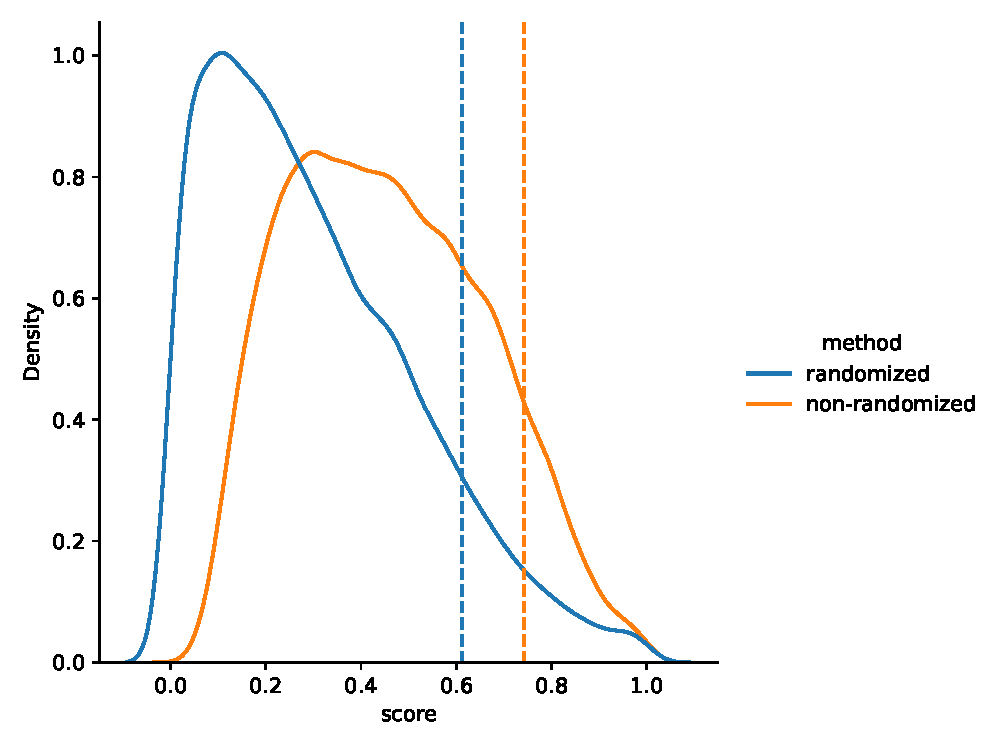
\includegraphics[width=\linewidth]{graphConformal/figures/aps_dist}
    \end{subfigure}
    \begin{subfigure}{0.7\linewidth}
        \centering
        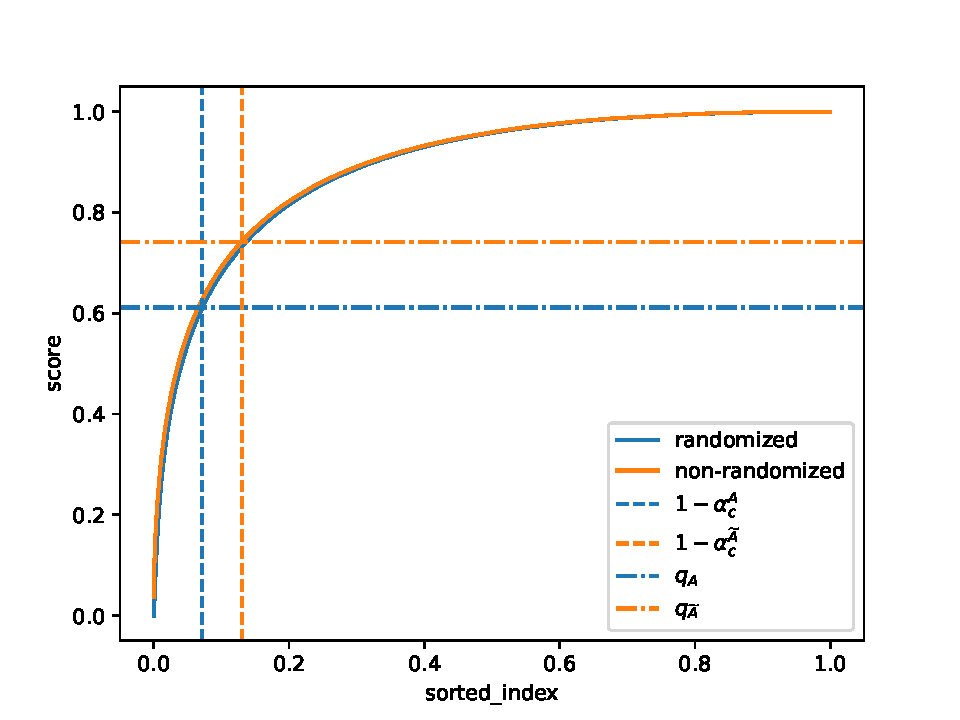
\includegraphics[width=\linewidth]{graphConformal/figures/aps_sorted}
    \end{subfigure}
    \caption{Figure showing the scores for an example dataset. (top) shows the shift in the quantile for $A$ and $\Tilde{A}$ for the correct class. (bottom) shows the shift $\alpha_c$ for $A$ and $\Tilde{A}$ using scores $A'$ for the incorrect classes.}
    \label{fig:APS:efficiency}
\end{figure}

%\pmcomment{empirical quantiles with epsilon}

%\begin{align*}
%   |S(\vx_{n+1}, u; \hat{\pi}, \tau_A)| - |\Tilda{S}(\vx_{n+1}; \hat{\pi}, \tau_{})|
%\end{align*}

\subsection{Notes on Transductive NAPS}
Neighborhood Adaptive Prediction Sets (NAPS) can construct predictive sets via Conformal Prediction under relaxed exchangeability (or non-exchangeability) assumptions~\cite{barber2023conformal}.
In the context of graphs, NAPS was initially implemented in the inductive setting~\cite{clarkson2023distribution}.
However, it can be used in the transductive setting as well~\cite{zargarbashi23conformal}. 
NAPS in the transductive setting is based on APS where $s_i = A(\vx_i, y_i, u_i;\hat{\pi}_i)$, or $A(\vx_i, y_i;\hat{\pi}_i)$ (depending on whether the randomized version is used), is computed for each node in $\gD_{\text{calib}}$. 
Using these scores, a weighted quantile is computed to produce the score threshold for prediction sets (Equation~\ref{eq:NAPS:quantile})
Unlike APS, the quantile is defined by placing weighted point masses ($\delta$) at each score from the calibration set under consideration for quantile computation.
The point mass at $+\infty$ indicates that the score for test node $n+1$ is unknown (and unbounded due to non-exchangeability), and thus, a point mass at the maximum value ($+\infty$) is required.%\ascomment{I want to state the intuitive reason for the infinite point mass since it was not clearly stated in the NAPS paper.} 
\begin{align}
    \hat{q}^{\text{NAPS}}_{n+1} = \text{Quantile}\bigg(1-\alpha, \bigg[\sum_{i\in\gD_{\text{calib}}}\Tilde{w}_{i}\cdot \delta_{s_{i}}\bigg] + \Tilde{w}_{n+1}\cdot \delta_{+\infty}\bigg)
    \label{eq:NAPS:quantile}
\end{align}

For NAPS to produce viable prediction sets, the weights, $w_i\in [0,1]$, for nodes under consideration in the calibration set must be chosen in a data independent fashion, i.e., they cannot leverage the feature vectors associated with the calibration nodes~\citep{barber2023conformal}.
NAPS leverages the graph structure to assign these weights, assigning non-zero weights to nodes within a k-hop neighborhood $\gN_{n+1}^k$ of the test node $v_{n+1}$.
%Since exchangeability is not assumed, a weight function leveraging graph homophily can be used to produce weights, $w_i\in [0,1]$, for nodes in the calibration set \cite{barber2023conformal}. 
The three implemented weight functions are uniform, $w_u(d_i) = 1$, hyperbolic $w_h(d_i) = \frac{1}{d_i}$, and exponential, $w_e(d_i) = 2^{-d_i}$ for nodes in the k-hop neighborhood, where $d_i$ is the distance from $v_{n+1}$ to $v_i \in \gV_{\text{calib}}$.
Formally, the weight function for each node, $v_i \in \gV_{\text{calib}}$ can be seen in Equation \ref{eq:NAPS:weight} below, where $w_x(d_i)$ is the selected weight function.
These weights are then normalized to compute $\Tilde{w}_i$ such that $\sum_{i\in\gD_{\text{calib}}} \Tilde{w}_i + \Tilde{w}_{n+1} = 1$ \cite{barber2023conformal}.
\begin{align}
    w_i = \begin{cases}
w_x(d_i), & i\in \gD_{\text{calib}}\cap\mathcal{N}_{n+1}^k\\
0,& i\in \gD_{\text{calib}}\setminus\mathcal{N}_{n+1}^k
\end{cases}
    \label{eq:NAPS:weight}
\end{align}

Using the NAPS quantile, $\hat{q}^{\text{NAPS}}_{n+1}$, the prediction sets can be constructed similarly to other Conformal Prediction algorithms.
Note that NAPS was originally designed for the inductive setting; transductive differs as non-zero weights are assigned to fewer nodes as only a subset of the graph nodes are assigned to be calibration nodes.
In the inductive setting, no exchangeability cannot be assumed and the entire graph prior to the test phase is considered as a calibration set leading to a larger number of non-zero weights.

\noindent \textbf{NAPS Implementation}
NAPS is computationally more expensive with regard to time and memory as a k-hop intersection must be computed for each test node.
We optimized this implementation using a batched approach that works with sparse tensors (Algorithm \ref{alg:NAPS:Quantile}).
Informally, the test nodes are first split up into batches. 
Then, for each batch, the distance to each node in the k-hop neighborhood is computed.
Following this, the weights function for the corresponding nodes are computed before computing the quantile for each node.
The batched approach ensures that sufficient memory is available for the necessary computations - especially for computing the distance to each node in the k-hop neighborhood without needing to densify a sparse graph.

\begin{algorithm}
\caption{NAPS Quantile Implementation}\label{alg:NAPS:Quantile}
\begin{algorithmic}[1]
\Procedure{NAPS\_Quantile}{$w,k,\calib,\test,\mathcal{D},\mathcal{S}_{\text{calib}},b,\alpha$}
    \State $\{\mathcal{B}_1,\mathcal{B}_2,\hdots,\mathcal{B}_b\}\gets \Call{\text{split}}{\test,b}$ \Comment{Split test nodes into b batches}
    \State $q\gets \Call{\text{zeros}}{\test,1}$\Comment{$q\in \mathbb{R}^{|\test| \times 1}$}
    \For{$\mathcal{B}_n \in \{\mathcal{B}_1,\mathcal{B}_2,\hdots,\mathcal{B}_b\}$}
        \State $\text{k\_hop} \gets \Call{\text{Sparse\_k\_hop}}{k,\mathcal{B}_n,\calib,\mathcal{D}}$\Comment{k\_hop $\in \mathbb{R}^{|\mathcal{B}_n|\times|\calib|}$}
        \State $\text{weights}\gets \Call{\text{compute\_weights}}{w,\text{k\_hop}}$\Comment{weights $\in \mathbb{R}^{|\mathcal{B}_n|\times|\calib|}$}
        \State $q[\mathcal{B}_n]\gets \Call{\text{compute\_quantile}}{1-\alpha,\text{weights},\mathcal{S}_{\text{calib}}}$
    \EndFor\label{NAPSquantileendwhile}
    \State \textbf{return} $q$\Comment{Return the quantiles for each test node}
\EndProcedure
\end{algorithmic}
\end{algorithm}

To ensure scalability for large graphs, all the computations until the quantile computation setep were done via sparse tensors. 
Algorithm \ref{alg:NAPS:SparseKHop} illustrates how the distance to each calibration node in the k-hop neighborhood can be computed via  sparse tensorr primitives.
The sign function based formulation uses the fact that subtracting $n+1$-hop paths from a matrix containing up to $n$ hops to ensure negative values at paths of length exactly $n+1$, with the rest being 0.
%To ensure that the minimum distance to nodes in the k-hop neighborhood is reported, the sign function is applied to the matrix containing paths exactly n hops away. This is subtracted from the matrix containing distances up to n-1 hops. A value can only be less than 0 after this subtraction if the corresponding index in the matrix containing distances up to n-1 hops was 0. Using this, the nodes that are at a minimum n hops away can be identified and added to the matrix containing distances to calibration nodes in the k-hop neighborhood. The described calculations can be done using sgn, and signbit (to check if an element is negative) in PyTorch.\ascomment{Shorted this paragraph}  

\begin{algorithm}
\caption{Sparse K Hop Neighborhood Implementation}\label{alg:NAPS:SparseKHop}
\begin{algorithmic}[1]
\Procedure{Sparse\_k\_hop}{$k,\mathcal{B},\calib,\mathcal{D}$}
    \State $\text{A}\gets \Call{\text{Get\_Adjacency}}{\mathcal{D}}$ \Comment{Adjacency of $\mathcal{D}$, A $\in \mathbb{R}^{|\mathcal{D}|\times|\mathcal{D}|}$}
    \State $\text{path\_n}\gets \text{A[$\mathcal{B},:$]}$\Comment{path\_n $\in \mathbb{R}^{|\mathcal{B}|\times|\mathcal{D}|}$ }
    \State $\text{k\_hop}\gets \text{path\_n[$:,\calib$]}$\Comment{k\_hop $\in \mathbb{R}^{|\mathcal{B}|\times|\calib|}$ }
    \For{$n \in \{2,3,\hdots,k\}$}
        \State $\text{path\_n} \gets (\text{path\_n})\text{A}$
        \State $\text{neg\_if\_n}\gets \text{k\_hop}-\Call{\text{sgn}}{\text{path\_n[$:,\calib$]}}$\Comment{negative value $\implies$ n hops away}
        \State $\text{in\_n\_hop}\gets (\text{neg\_if\_n}<0)\times n$ \Comment{Nodes that are a min distance of n}
        \State $\text{k\_hop} \gets \text{k\_hop} + \text{in\_n\_hop}$
    \EndFor\label{khopendwhile}
    \State \textbf{return} $\text{k\_hop}$\Comment{$\forall_{i,j}\, \text{\textbf{If} dist($i,j$)}  \leq k \text{ \textbf{then} k\_hop[$i,j$]} = \text{dist}(i,j), \text{\textbf{else} k\_hop[$i,j$]}=0$}
\EndProcedure
\end{algorithmic}
\end{algorithm}

\subsection{Diffusion Adaptive Prediction Sets}
The Diffusion Adpative Prediction Sets (DAPS) approach for conformal node classification on graphs was introduced by \citet{zargarbashi23conformal}.
The intuition behind DAPS is that the prevalence of homophily in graphs implies that the non-conformity scores for two connected scores should be related.
DAPS uses a diffusion step to capture this relationship and uses the non-conformity scores modified by diffusion to generate the prediction sets.
Formally, suppose $s(v, y)$ is a point wise non-conformity score for a node $v$ and label $y$ (e.g., TPS or APS)
\[
    \hat{s}(v, y) = (1 - \lambda) s(v, y) + \frac{\lambda}{|
    \gN_v|} \sum\limits_{u \in \gN_v} s(u, y)
\]
where $\gN_v$ is the 1-hop neighborhood of $v$ and $\lambda \in [0, 1]$ is a hyperparameter controlling the diffusion.

\citet{zargarbashi23conformal} use the APS score as the point wise score in diffusion process as it is adaptive and uniformly distribution in $[0, 1]$ under oracle probability.
However, as we noted earlier, using class wise thresholds provides a mechanism to produce adaptive scores from TPS as well.
Thus, we create DTPS, a variation of DAPS using TPS-Classwise scores as the point wise scores in the diffusion process.

\subsection{Conformalized GNN}
\begin{figure}
    \centering
    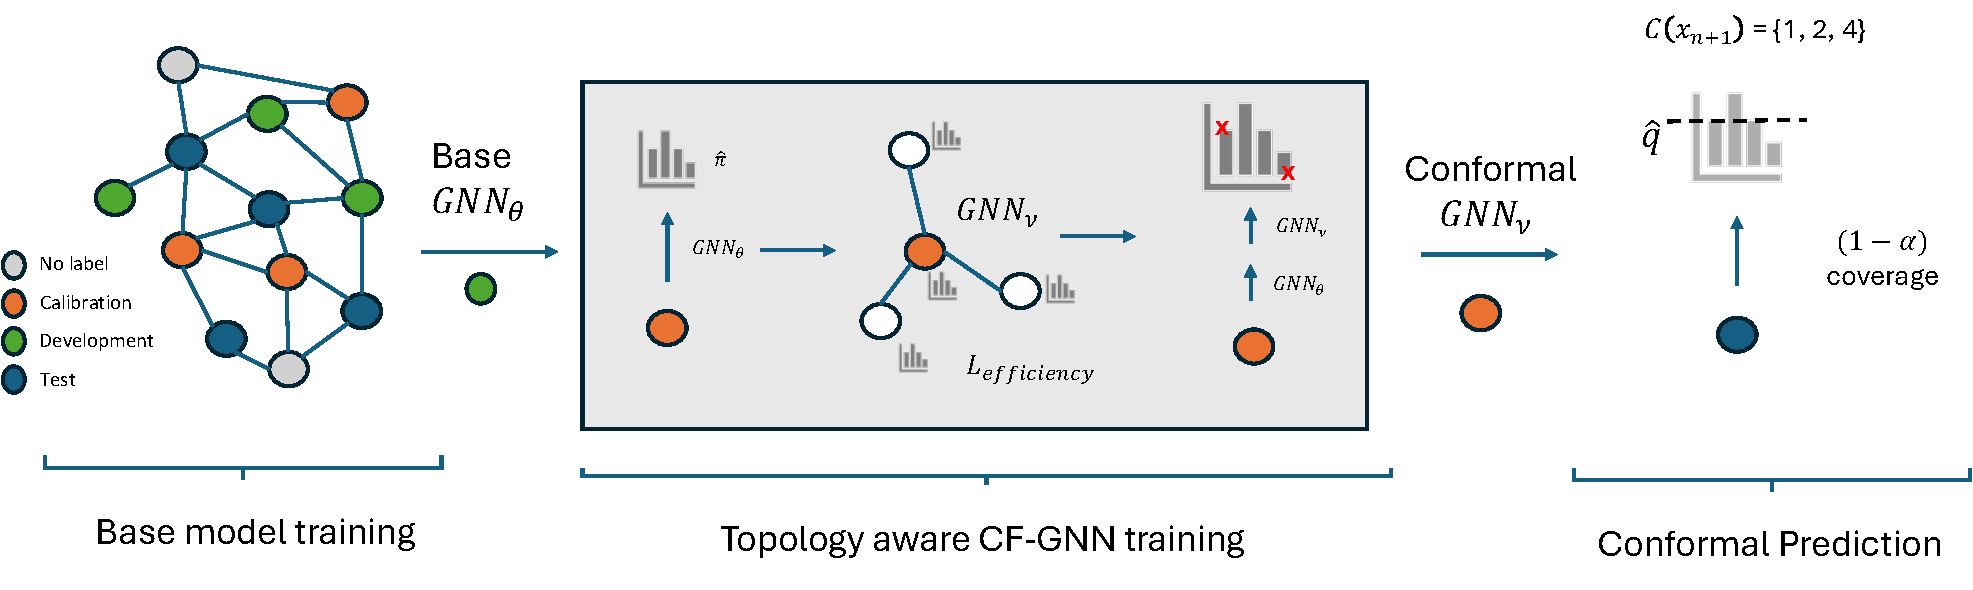
\includegraphics[width=\linewidth,alt={CF-GNN three stage training procedure.}]{graphConformal/figures/CFGNN.pdf}
    \caption{Procedure for training CF-GNN. First (left), the base model is trained on the training set. Then, (middle) the CF-GNN is trained to maximize efficiency over the calibration set. Finally , (right) the non-conformity scores from the combined models are used to generate the prediction sets.}
    \label{fig:conformalized_gnn}
\end{figure}

Conformalized GNN (CFGNN)~\citep{huang2024uncertainty} is a GNN-based approach for conformal prediction.
The authors observed that inefficiencies are correlated between nodes having similar neighborhood topology in a graph setting.
They use a GNN during the calibration phase, which is trained to correct the scores output from the base model such that the corrected scores maximize the efficiency of the conformal prediction.
For classification-based losses, CFGNN utilizes the fact that all steps in the conformal prediction stage for computing the prediction sets (non-conformity score computation, quantile computation, thresholding) can be expressed as differentiable operations.
Thus, a GNN can be trained directly using efficiency as a loss function.
Figure~\ref{fig:conformalized_gnn} provides a high-level overview of the CFGNN approach.

\noindent \textbf{CFGNN Implementation Improvements}
The choice of the conformal loss during calibration and test plays an important role in determining the overall performance of the CFGNN.
\citet{huang2024uncertainty} use a TPS loss for the calibration phase and the non-randomized APS loss for constructing the final prediction sets.
Our preliminary experiments (Figure~\ref{fig:CFGNN:preliminary}) with replacing the APS loss with a randomized version demonstrated that these losses must be tuned carefully to ensure that the CFGNN is able to improve upon the base models non-conformity scores.
Some improvements shown in CFGNN (Figure~\ref{fig:CFGNN:preliminary}, right) get nullified when the randomized APS loss is used (left).

Additionally, CFGNN uses full batch training which makes it unable to scale for larger graphs.
We implemented a batched version of CFGNN to ensure that it can be used for larger graphs.
Finally, to speed up computation, we allow the use of cached outputs from the base model rather than having to sample neighbors for both the base model and the CFGNN.
Algorithm~\ref{alg:cfgnn:catching} shows these improvements in the CFGNN implementation.
We cache the output of the base $\text{GNN}_\theta$ prior to running the CFGNN training loop, allowing the sampling of $m$ layers of message passing graphs rather than $m + l$ layers required by the baseline CFGNN.
In addition, we control the batch size $b$ when sampling neighbors.
These changes significantly speeds up the computation for CFGNNs (see Section~\ref{sec:conformal:results:cfgnn:runtime} for speedup results).
\begin{algorithm}
    \caption{CFGNN batching + caching implementation}\label{alg:cfgnn:catching}
    \begin{algorithmic}[1]
    \State $\text{GNN}_{\theta}$ \Comment{$l$ layer base GNN, with pretrained, fixed weights}
    \State $\text{GNN}_{\phi} \gets \Call{\text{RandomInitialization}}{\phi}$ \Comment{$m$ layer trainable CFGNN}
    \If{cache\_base}
        \State $\gX \gets \text{GNN}_{\theta}(\gG, \gX)$ \Comment{Compute base model output}
    \EndIf
    \Procedure{CFGNNTrainStep}{$\calib, \gG, \gX$}
        \State $\gB \gets \Call{\text{SampleBatch}}{\calib, b}$ \Comment{batch size $b$ is $|\calib|$ for base CFGNN}
        \If{cache\_base}
            \State{$\text{CFFeats, CFMsgGraphs} \gets \Call{\text{ NeighborSampler}}{\gB, m, \gX}$}
        \Else
            \State{$\text{Feats, MsgGraphs} \gets \Call{\text{NeighborSampler}}{\gB, l + m, \gX}$}
            \State{$\text{CFFeats} \gets \text{GNN}_\theta(\text{Feats}, \text{MsgGraphs}_{0, \dots, m-1})$}
            \State{$\text{CFMsgGraphs} \gets \text{MsgGraphs}_{m, \dots, m+l-1}$}
        \EndIf
        \State $\text{scores} \gets \text{GNN}_{\phi}(\text{CFFeats}, \text{CFMsgGraphs})$
        \State $\gL \gets \Call{\text{ConformalLoss}}{\text{scores}, \gB}$
        \State $\Call{\text{UpdateWeights}}{\text{GNN}_\phi, \gL}$
    \EndProcedure
    \end{algorithmic}
\end{algorithm}


\begin{figure}
    \centering
    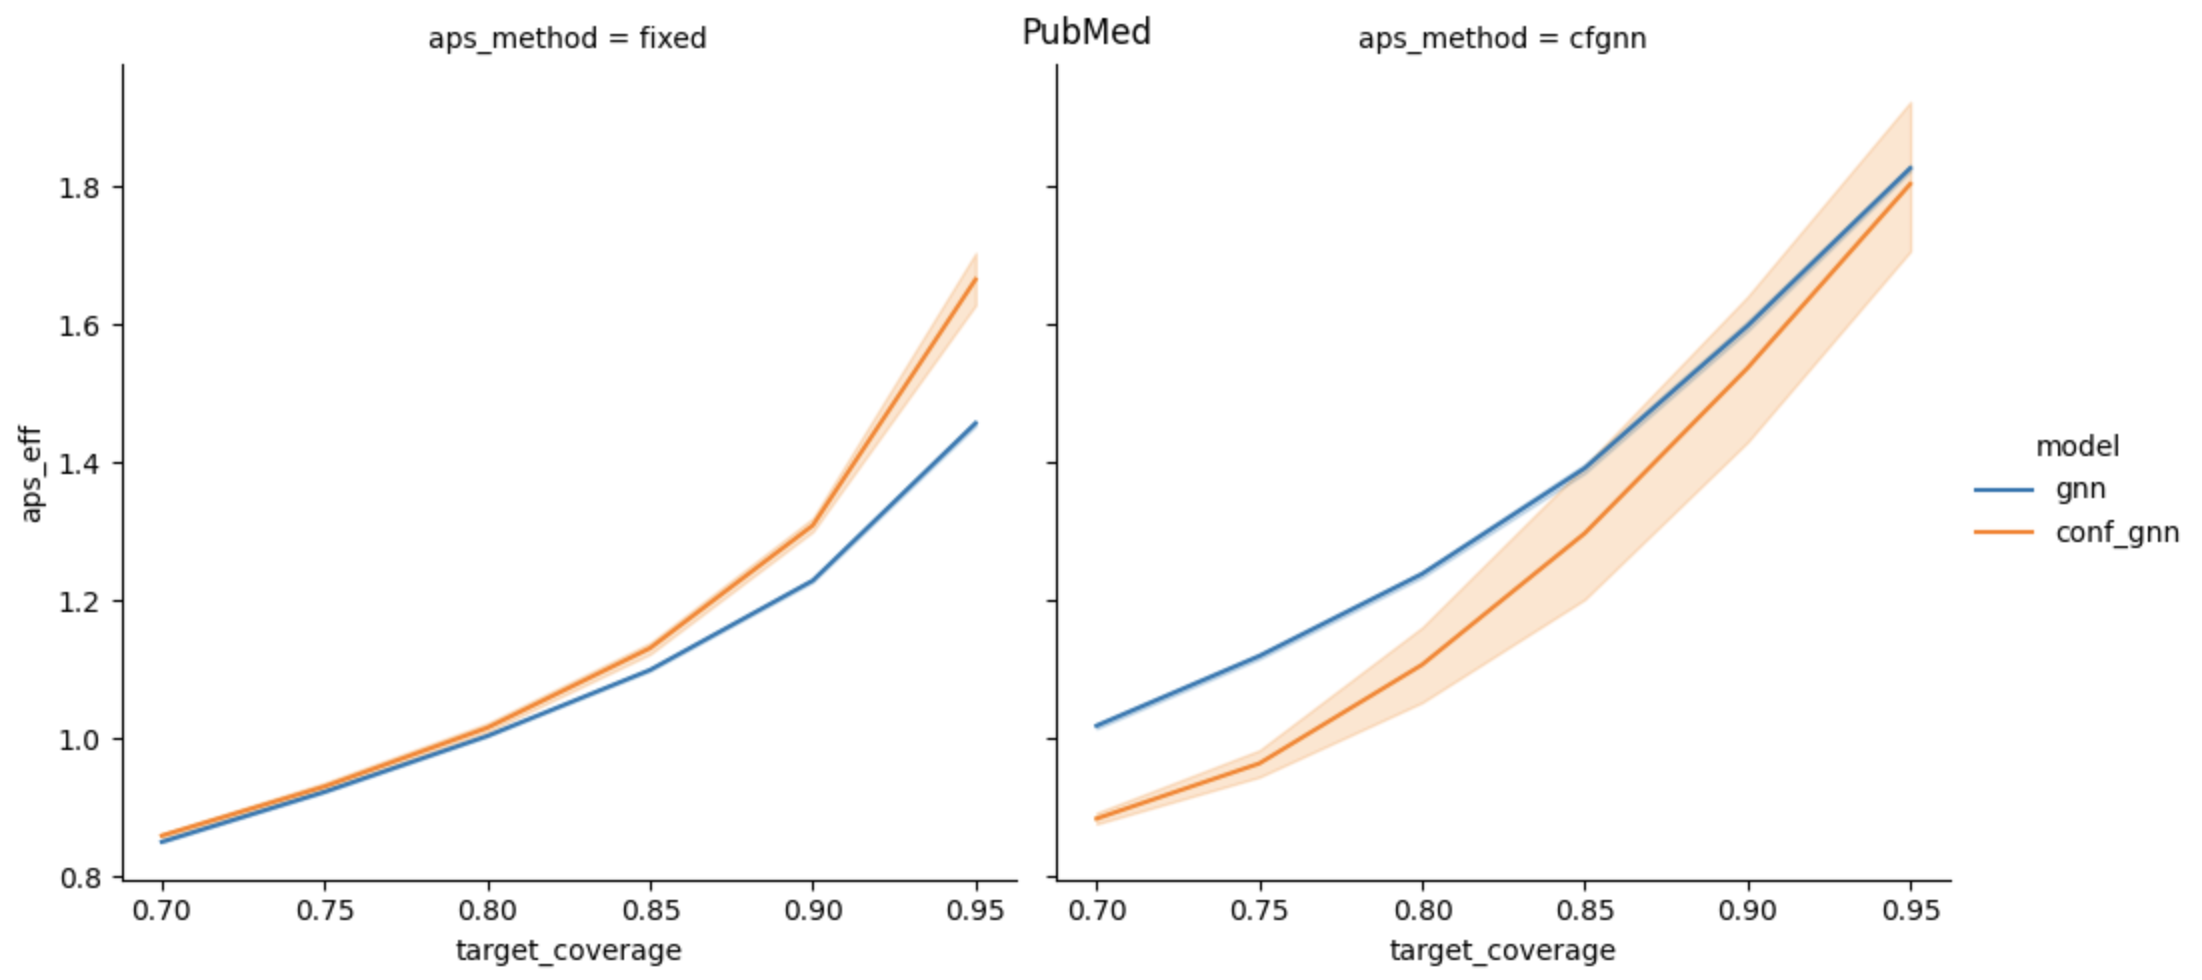
\includegraphics[width=0.8\linewidth,alt={Preliminary results on effciency comparison with APS vs CFGNN.}]{graphConformal/figures/PubMed_CF.png}
    %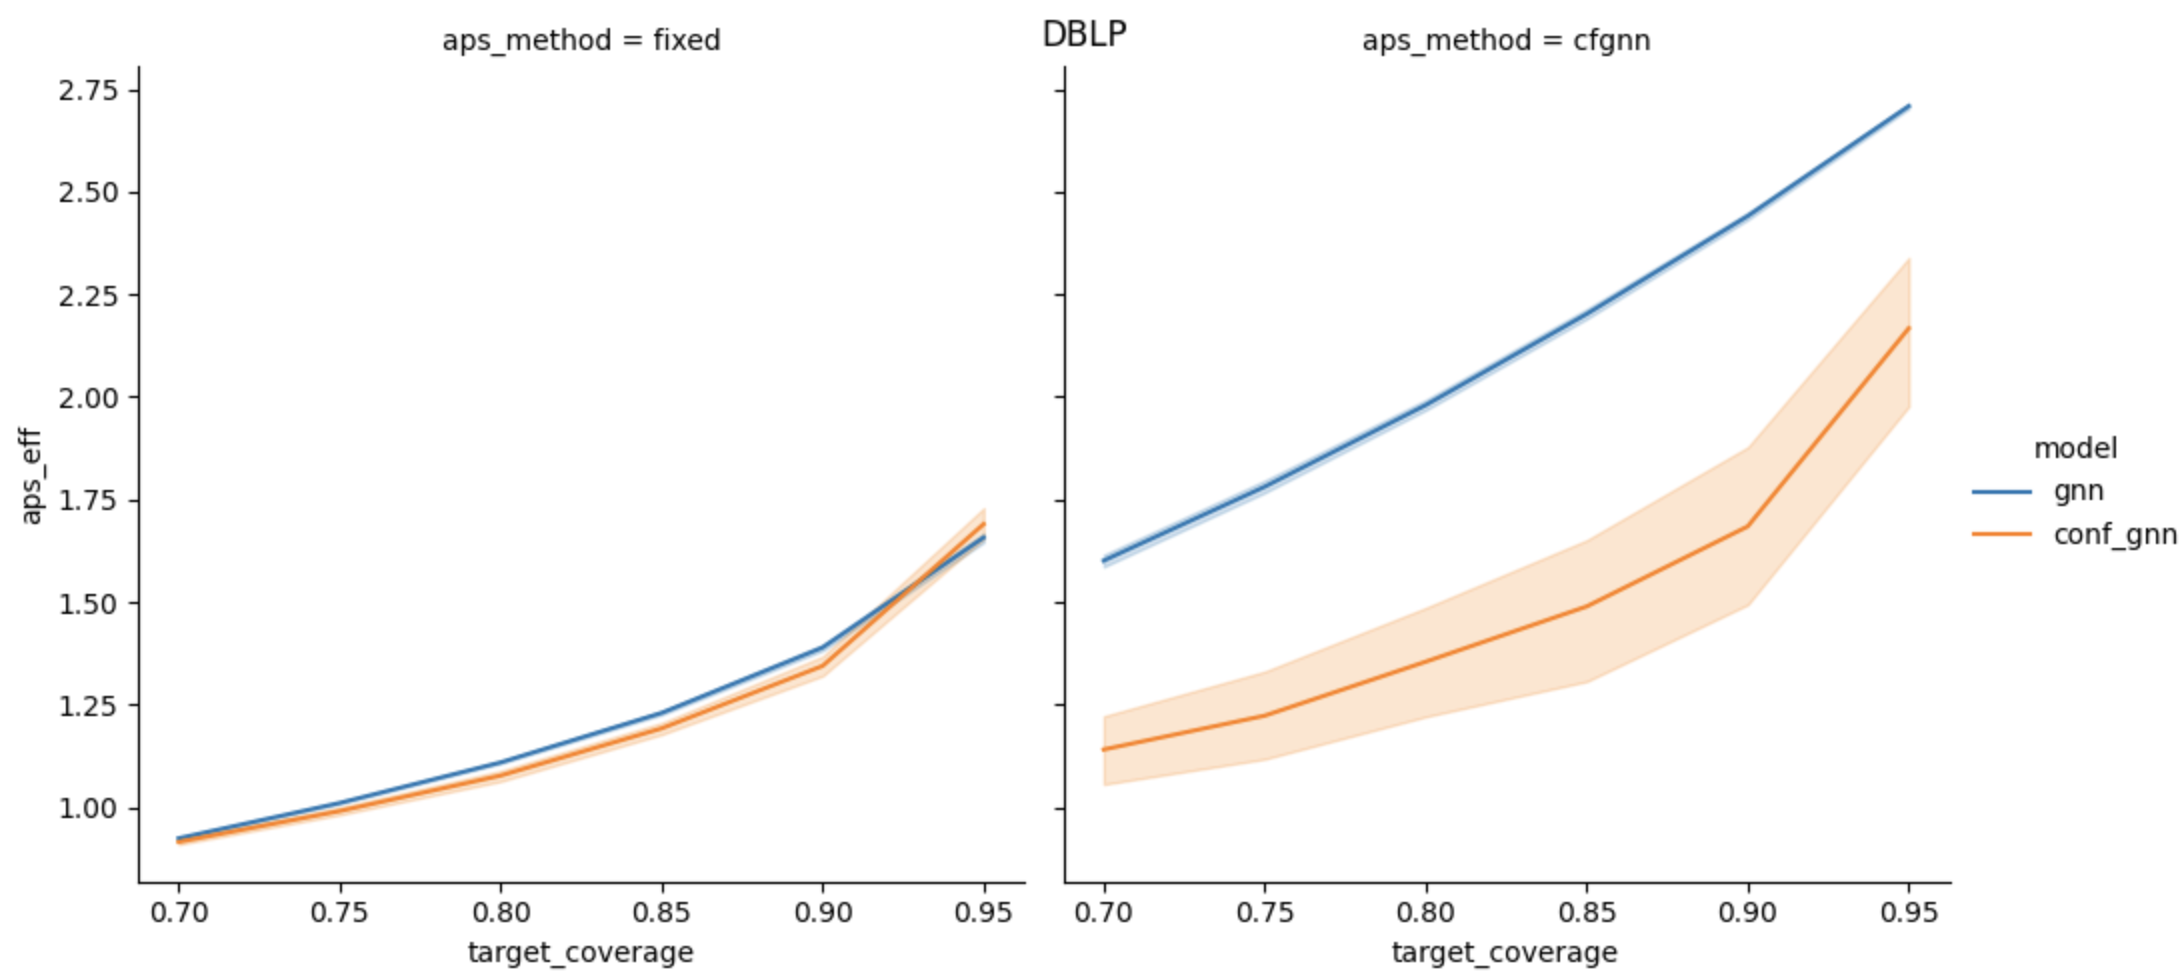
\includegraphics[width=0.7\linewidth]{graphConformal/figures/DBLP_CF.png}
    \caption{Comparing the efficiency (average output set size) for the base model and the CFGNN on the Pubmed dataset. The plot on the left uses the fixed version of the APS score (with randomized sets) while on the right uses the non-randomized version.}
    \label{fig:CFGNN:preliminary}
\end{figure}






\begin{subappendices}
    \section{Optimal $\tau$ for APS}
\label{appx:APS:tau}
For simplicity, assume that the probabilities are distinct.

From the definition of $A$ \eqref{eq:APS:score}
\begin{align*}
    A(\vx, y, u;\hat{\pi}) &= \min\{\tau \in [0, 1]: y \in S(\vx, u; \hat{\pi}, \tau)\}
\end{align*}
Define 
\[
\Sigma_{\hat{\pi}}(\vx, m) = \sum\limits_{i=1}^m \hat{\pi}_{(i)}(\vx)
\]
From the definition of $S(\vx, u; \hat{\pi}, \tau)$ from \eqref{eq:APS:S}, conisder the following cases:

\textbf{Case 1:} $\tau = \Sigma_{\hat{\pi}}(\vx, r_y)$, then $L(x; \hat{\pi}, \tau) = y$ and thus, $V(\vx; \pi, \tau) = 0$.
Thus $\Pr[u > V(\vx; \pi, \tau)] = 1$ and hence, $P[y \in S(\vx, u; \hat{\pi}, \tau)] = 1$.

\textbf{Case 2:} $\tau = \Sigma_{\hat{\pi}}(\vx, r_y-1)$, then $y \not\in S(\vx, u, \hat{\pi}, \tau)$ in either case, since only classes with $\hat{\pi}_i(\vx) > \hat{\pi}_y(\vx)$ could be included. \pmcomment{This is the edge case where tie breaking is required for a completely general proof.}

\textbf{Case 3:} $\tau = \Sigma_{\hat{\pi}}(\vx, r_y) - \varepsilon \hat{\pi}_y$.
Then we have $L(x; \hat{\pi}, \tau) = y$ again, and 
\begin{align*}
    V(\vx; \pi, \tau) &= \frac{1}{\hat{\pi}_y(\vx)}\left\{ \left[ \sum_{j=1}^{r_y} \hat{\pi}_{(j)}(\vx) \right] - \tau \right\} \\
                      &= \frac{1}{\hat{\pi}_y(\vx)}\left\{ \left[ \sum_{j=1}^{r_y} \hat{\pi}_{(j)}(\vx) \right] - (\Sigma_{\hat{\pi}}(\vx, r_y) - \varepsilon \hat{\pi}_y) \right\}\\
                      &= \varepsilon
\end{align*}
For $y$ to be included in $S(\vx, u; \hat{\pi}, \tau)$, we would require that $u \geq V(\vx; \pi, \tau)$, i.e., $u \geq \varepsilon$. 
We want the minimal $\tau$, which is equivalent to maximizing $\varepsilon$. 
Thus, $\tau = \Sigma_{\hat{\pi}}(\vx, r_y) - u \hat{\pi}_y$ is the required solution.

\subsection{Non-randomized set}
The inclusion criterion for the score given the threshold $\tau$ is $\Tilde{A}(\vx, y; \hat{pi}) \leq \tau$

To include the currct label $y_i$ while minimizing the chosen threshold $\tau$, we would require $\tau = \sum\limits_{j=1}^{r_{y_i}} \hat{\pi}_{(j)}(\vx)$ 
\end{subappendices}


\chapter{Stylometry on the Darkweb}
\label{chp:sysml}

\todo{Cross training as curriculum learning}
Darknet market forums are frequently used to exchange illegal goods and services between parties who use encryption to conceal their identities. The Tor network is used to host these markets, which guarantees additional anonymization from IP and location tracking, making it challenging to link across malicious users using multiple accounts (sybils). Additionally, users migrate to new forums when one is closed further increasing the difficulty of linking users across multiple forums. We develop a novel stylometry-based multitask learning approach for natural language and model interactions using graph embeddings to construct low-dimensional representations of short episodes of user activity for authorship attribution. We provide a comprehensive evaluation of our methods across four different darknet forums demonstrating its efficacy over the state-of-the-art, with a lift of up to 2.5X on Mean Retrieval Rank and 2X on Recall@10.

\section{Introduction}
\label{sec:sysml:intro}
Crypto markets are \textit{``online forums where goods and services are exchanged between parties who use digital encryption to conceal their identities''}~\citep{martin2014drugs}. 
  They are typically hosted on the Tor network, which guarantees  anonymization in terms of IP and location tracking. 
  The identity of individuals on a crypto-market is associated only with a username; therefore, building trust on these networks does not follow conventional models prevalent in eCommerce. 
 % \textit{``The formation of trust, and the ultimate acceptance of the new user within the community, is often constructed via prospective users demonstrating their legitimacy through action''}~\cite{lacey2015s}. 
  Interactions on these forums are facilitated by means of text posted by their users. 
  This makes the analysis of textual style on these forums a compelling problem.
  % TODO add a paragraph on why darkweb stylometry is important from the criminal side
  
  Stylometry is the branch of linguistics concerned with the analysis of authors' style.
  Text stylometry was initially popularized in the area of forensic linguistics, specifically to the problems of author profiling and author attribution~\citep{juola2008authorship,rangel2013overview}.
  Traditional techniques for authorship analysis on such data rely upon the existence of long text corpora from which features such as the frequency of words, capitalization, punctuation style, word and character n-grams, function word usage can be extracted and subsequently fed into any statistical or machine learning classification framework, acting as an author's `signature'. 
  However, such techniques find limited use in short text corpora in a heavily anonymized environment.
 
  
  Advancements in using neural networks for character and word-level modeling for authorship attribution aim to deal with the scarcity of easily identifiable `signature' features and have shown promising results on shorter text~\citep{shrestha2017convolutional}. 
  \citet{andrews2019learning} drew upon these advances in stylometry to propose a model for building representations of social media users on Reddit and Twitter. Motivated by the success of such approaches, we develop a novel methodology for building authorship representations for posters on various darknet markets. 
  Specifically, our key contributions include: 
  
  \noindent \textbf{First}, a {\it representation learning} approach that couples temporal content stylometry with access identity (by levering forum interactions via \textit{meta-path graph context information}) to model and enhance user (author) representation; 

  \noindent \textbf {Second}, a novel framework for training the proposed models in a \textit{multitask setting} across multiple darknet markets, 
  using a small dataset of labeled migrations, 
  to refine the representations of users within each individual market, while also providing a method to correlate users across markets; 
  
\noindent \textbf{Third}, a detailed drill-down {\it ablation study} discussing the impact of various optimizations and highlighting the benefits of both graph context and multitask learning  on forums associated with four darknet markets - \textit{Black Market Reloaded}, \textit{Agora Marketplace}, \textit{Silk Road}, and \textit{Silk Road 2.0} -
 when compared to the state-of-the-art alternatives.
  %Additionally, large pre-trained language models such as BERT and XLM~\cite{devlin2018bert,conneau2019unsupervised} have made it possible to adapt contextual representations learned from large corpora to new and challenging multi-language text analysis problems.
  
  

\section{Related Work}
%We describe related work in the domain of darknet market analysis, authorship attribution,  and multitask learning for text.
\label{sec:sysml:related}
\noindent {\bf Darknet Market Analysis:}
Content on the dark web includes resources devoted to illicit drug trade, adult content, counterfeit goods and information, leaked data, fraud, and other illicit services~\citep{biryukov2014content}. 
Also included are forums discussing politics, anonymization, and cryptocurrency. 
\citet{biryukov2014content} found that while a vast majority of these services were in English (about $84\%$), a total of about 17 different languages were detected.
%(e.g.  Indo-European, Slavic, Sino-Tibetan, and Afro-Asiatic languages). 
Analysis of the volume of transactions and number of users on darknet markets indicates that they are resilient to closures; rapid migrations to newer markets occur when one market shuts down~\citep{elbahrawy2019collective}.
%, and the total number of users remains relatively unaffected. 

\begin{comment}
\textcolor{teal}{Recent work analyzed vendor listings to identify sybil vendors and link them across markets~\cite{kumar2020edarkfind,tai2019adversarial}. 
These works focus on the textual content of the vendor listing, along with heuristics based on the specific items on sale. 
\citet{xiangwen2018you} integrated features from product photos available in listings to aid this analysis. However, most darknet markets also have associated forums where users discuss vendor identities and build trust~\cite{lorenzo2018know}, but these forums discussions remain underutilized for identity analysis, which is the focus of our work.} 
\end{comment}

\todo{TODO: Weird DBLP cites. }
Recent work~\cite{fan2018automatic,hou2017hindroid,fu2017hin2vec,dong2017metapath2vec} has levered the notion of a heterogeneous information network (HIN) embedding to improve graph modeling, where different types of nodes, relationships (edges) and paths can be represented through typed entities.  
\citet{zhang2019style} used a HIN to model marketplace vendor sybil\footnote{a single author can have multiple users accounts which are considered as \textit{sybils}} accounts on the darknet, where each node representing an object is associated with various features (e.g. content, photography style, user profile and drug information).
%some attributes of its type. They extracted various features based on textual content, photography styles, user profiles, and drug information and adopted an attribute-aware sampling method, which enabled two objects of the same type with similar attributes to appear together more frequently in the sampled paths. 
Similarly,~\citet{kumar2020edarkfind} proposed a multi-view unsupervised approach which incorporated features of text content, drug substances, and locations to generate vendor embeddings. We note that while such efforts~\cite{zhang2019style,kumar2020edarkfind} are related to our work, there are key distinctions. 
First, such efforts focus only on vendor sybil accounts. 
Second, in both cases, they rely on a host of multi-modal information sources (photographs, substance descriptions, listings, and location information) that are not readily available in our setting -  limited to forum posts.
Third, neither effort exploits multitask learning. 

\noindent {\bf Authorship Attribution of Short Text:}
\citet{kim2014convolutional} introduced convolutional neural networks (CNNs) for text classification.
Follow-up work on authorship attribution~\cite{ruder2016character, shrestha2017convolutional} leveraged these ideas to demonstrate that CNNs outperformed other models, particularly for shorter texts. 
%Additionally, weight sharing between the convolutional filters allow models with fewer parameters to be trained for text classification. 
The models proposed in these works aimed at balancing the trade-off between vocabulary size and sequence length budgets based on tokenization at either the character or word level.
Further work on subword tokenization~\cite{sennrich2016neural}, especially byte-level tokenization, have made it feasible to share vocabularies across data in multiple languages. 
Models built using subword tokenizers have achieved good performance on authorship attribution tasks for specific languages (e.g., Polish~\cite{grzybowski2019sparse}) and also across multilingual social media data~\cite{andrews2019learning}.
Non-English as well as multilingual darknet markets have been increasing in number since 2013~\cite{ebrahimi2018detecting}.
Our work builds upon all these ideas by using CNN models and experimenting with both character and subword level tokens.


\noindent {\bf Multitask learning (MTL):}
MTL~\cite{caruana1997multitask}, aims to improve machine learning models' performance on the original task by jointly training related tasks. 
MTL enables deep neural network-based models to better generalize by sharing some of the hidden layers among the related tasks. 
%multitask learning has been widely applied in various fields, such as natural language processing~\cite{liu2019multi}, drug discovery~\cite{ramsundar2015massively}, and computer vision~\cite{zhang2016joint}. 
Different approaches to MTL can be contrasted based on the sharing of parameters across tasks - strictly equal across tasks (hard sharing) or constrained to be close (soft-sharing)~\cite{ruder2017an}.
Such approaches have been applied to language modeling~\cite{howard2018universal}, machine translation~\cite{dong2015multi}, and dialog understanding~\cite{rastogi2018multi}.
%To the best of our knowledge, we are the first to propose the use of multitask learning for stylometry on the dark web.  
%\subsection{Graph Augmented Text Models}
% HIN (Your style your identity)
% Knowledge Base + generation (Pranav will add this)\textcolor{blue}{SP: May want to shorten this since our work is really not a HIN-like effort. The risk is we may be asked to compare with these strategies and that is not the point of our effort.\\ }
%\textcolor{red}{\cite{zhang2019style} focused on leveraging both text and associated network data to jointly model the darknet. They created an attributed heterogeneous network where each node is of different types, and then learned node representations with an attribute-aware sampling rule. Our work shares the idea of integration of text and graph structure of associated forums, but we have a different methodology: we learn representations for both text and other attributes and use their combinations as the final embedding.} \textcolor{red}{Recent works such as~\cite{zhang2019style} focused on leveraging text with associated network data to jointly model the darknet. To better model the relationships between different types of objects in the associated graph, existing works like~\cite{fan2018automatic,hou2017hindroid} usually construct a heterogeneous information network (HIN) in which there are different types of nodes and edges. Many HIN embedding methods~\cite{fu2017hin2vec,dong2017metapath2vec} have been proposed to learn the node representations from the relationships within the network. Instead of only using structural information, \cite{zhang2019style} proposed to create an attributed HIN where each node representing an object is associated with some attributes of its type. They extracted various features based on writing and photography styles and adopted an attribute-aware sampling rule which allows two objects of same type with similar attributes to be more likely to appear together in the sampled path instances. Our work shares the idea of integration of text and graph structure of associated forums, but we have a different methodology: we learn representations for both text and other attributes and use their combinations as the final embedding.}

\section{Datasets}
\label{sec:sysml:dataset}
\noindent \citet{munksgaard2016mixing} studied the politics of darknet markets using structured topic models on the forum posts across six  large markets.
We start with this dataset and perform basic pre-processing to clean up the text for our purposes. We focus on four of the six markets - \textit{Silk Road} (\textbf{SR}), \textit{Silk Road 2.0}~({\textbf{SR2}}), \textit{Agora Marketplace}~(\textbf{Agora}), and \textit{Black Market Reloaded} (\textbf{BMR}). 
We exclude `The Hub'  as it is not a standard forum but an `omni-forum'~\cite{munksgaard2016mixing} for discussion of other marketplaces and has a significantly different structure, which is beyond the scope of this work.
We also exclude `Evolution Marketplace' since none of the posts had PGP information present in them and thus were unsuitable for migration analysis.
%These markets are henceforth abbreviated SR, SR2, Agora, and BMR, respectively.

\noindent \textbf{Pre-processing}
We add simple regex and rule based filters to replace quoted posts (i.e., posts that are begin replied to), PGP keys, PGP signatures, hashed messages, links, and images each with different special tokens (\texttt{[QUOTE]}, \texttt{[PGP PUBKEY]}, \texttt{[PGP SIGNATURE]}, \texttt{[PGP ENCMSG]}, \texttt{[LINK]}, \texttt{[IMAGE]}).
We retain the subset of users with sufficient posts to create at least two episodes worth of posts. In our analysis, we focus on episodes of up to 5 posts. %(i.e., threshold: users with $\geq$ 10 posts).
To avoid leaking information across time, we split the dataset into approximately equal-sized train and test sets with a chronologically midway splitting point such that half the posts on the forum are before that time point.
Statistics for data after pre-processing is provided in Table~\ref{tab:dataset_stats}. Note that the test data can contain authors not seen during training.

\begin{table}[htbp]
    \centering
    \begin{tabular}{ccccc}
    \toprule
         Market &  Train Posts & Test Posts & \#Users train & \#Users test \\
    \midrule
         SR & 379382 & 381959 & 6585 & 8865\\
         SR2 & 373905 & 380779 &  5346 & 6580 \\
         BMR & 30083 &30474 & 855 & 931\\
         Agora & 175978 & 179482 & 3115 & 4209\\
    \bottomrule
    \end{tabular}
    \caption{Dataset Statistics for Darkweb Markets.}
    \label{tab:dataset_stats}
\end{table}


\noindent \textbf{Cross-dataset Samples} 
Past work has established PGP keys as strong indicators of shared authorship on darkweb markets~\cite{tai2019adversarial}. 
To identify different user accounts across markets that correspond to the same author, we follow a two-step process. 
First, we select the posts containing a PGP key, and then pair together users who have posts containing the same PGP key. 
Following this, we still have a large number of potentially incorrect matches (including scenarios such as information sharing posts by users sharing the PGP key of known vendors from a previous market). 
We manually check each pair to identify matches that clearly indicate whether the same author or different authors posted them, leading to approximately 100 reliable labels, with 33 pairs matched as migrants across markets.


\section{Methodology: \SYSMLmethodname{} Framework}
\label{sec:sysml:method}
Motivated by the success of social media user modeling using combinations of multiple posts by each user~\cite{andrews2019learning,noorshams2020ties}, we model posts on darknet forums using \textit{episodes}.
Each \textit{episode} consists of the textual content, time, and contextual information from multiple posts. 
A neural network architecture $f_{\theta}$ maps each episode to combined representation $e \in \mathbbm{R}^E$.
The model used to generate this representation is trained on various metric learning tasks characterized by a second set of parameters $g_{\phi}: \mathbbm{R}^E \xrightarrow[]{} \mathbbm{R}$.
We design the metric learning task to ensure that episodes having the same author have \textit{similar} embeddings.
Figure~\ref{fig:main_workflow} describes the architecture of this workflow and the following sections describe the individual components and corresponding tasks. 
Note that our base modeling framework is inspired by the social media user representations built by \citet{andrews2019learning} for a single task. 
We add meta-path embeddings and multitask objectives to enhance the capabilities of 
%this base model within 
\SYSMLmethodname{}. 
Our implementation is available at: \url{https://github.com/pranavmaneriker/SYSML}.

\begin{figure}[!htbp]
    \centering
    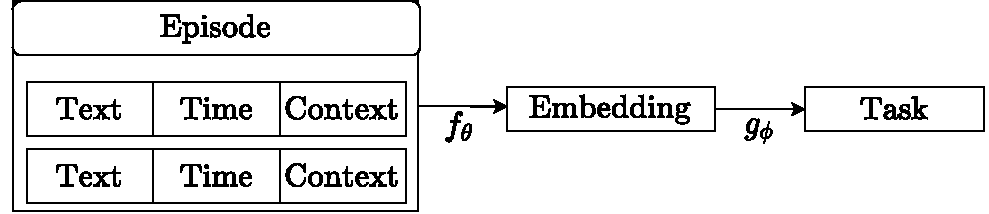
\includegraphics[width=\linewidth]{sysml/figures/MainFlowchart.pdf}
    \caption{Overall \SYSMLmethodname{} Workflow.}
    \label{fig:main_workflow}
\end{figure}

\subsection{Component Embeddings}
Each episode $e$ of length $L$ consists of multiple tuples of texts, times, and contexts 
\[
    e = \{(t_i, \tau_i, c_i) | 1 \leq i \leq L\} 
\]. 
Component embeddings map individual components to vector spaces. 
All embeddings are generated from the forum data only; no pretrained embeddings are used.

\noindent \textbf{Text Embedding} First, we tokenize every input text post using either a character-level or byte-level tokenizer. 
A one-hot encoding layer followed by an embedding matrix $E_t$ of dimensions $|V| \times d_t$ where $V$ is the token vocabulary and $d_t$ is the token embedding dimension embeds an input sequence of tokens $T_0$, $T_1$, $\dots, T_{n-1}$.
We get a sequence embedding of dimension $n \times d_t$. 
Following this, we use $f$ sliding window filters, with filters sized $F = \{2, 3, 4, 5\}$ to generate feature-maps which are then fed to a max-over-time pooling layer, leading to a $|F| \times f$ dimensional output (one per filter).
Finally, a fully connected layer generates the embedding for the text sequence, with output dimension $d_t$. 
A dropout layer prior to the final fully connected layer prevents overfitting, as shown in Figure~\ref{fig:kim_cnn}. 
\begin{figure}
    \centering
    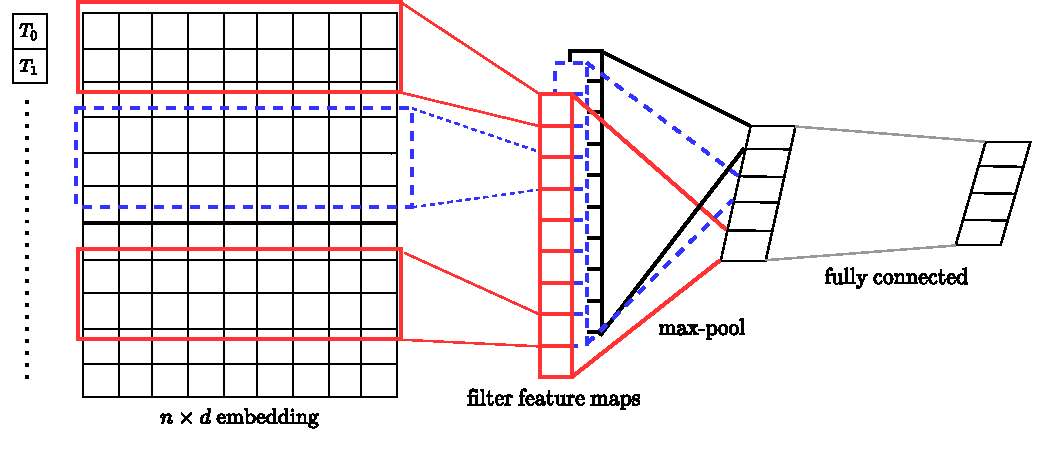
\includegraphics[width=\linewidth]{sysml/figures/TextCNN.pdf}
    \caption{Text Embedding CNN \cite{kim2014convolutional}.}
    \label{fig:kim_cnn}
\end{figure}

\noindent \textbf{Time Embedding} 
The time information for each post corresponds to when the post was created and is available at different granularities across darknet market forums. 
To have a consistent time embedding across different granularities, we only consider the least granular available date information (date) available on all markets.
We use the day of the week for each post to compute the time embedding 
by selecting the corresponding embedding vector of dimension $d_{\tau}$ from the matrix $E_w$.
%from a $7 \times d_{\tau}$ dimensional embedding matrix $E_w$ for a final embedding of dimension $d_{\tau}$.

\noindent \textbf{Structural Context Embedding} The context of a post refers to the threads that it may be associated with. 
Past work~\cite{andrews2019learning} used the subreddit as the context for a Reddit post.
In a similar fashion, we encode the subforum of a post as a one-hot vector and use it to generate a $d_c$ dimensional context embedding. 
In the previously mentioned work, this embedding is initialized randomly.
We deviate from this setup and use an alternative approach based on a \textit{heterogeneous graph} constructed from forum posts to initialize this embedding. 

\begin{definition}[Heterogeneous Graph]
A heterogeneous graph $G = (V, E, T)$ is one where each node $v$ and edge $e$ are associated with a `type' $T_i \in T$, where the association is given by mapping functions $\phi(v): V \rightarrow T_V$, $\psi(e): E \rightarrow T_E$, where $|T_V| + |T_E| > 2$
\end{definition}


The constraint on $T_{V,E}$ ensures that at least one of $T_V$ and $T_E$ have more than one element (making the graph heterogeneous). Specifically, we build a graph in which there are four types of nodes: user (U), subforum (S), thread (T), and post (P), and each edge indicates either a post of new thread (U-T), reply to existing post (U-P) or an inclusion (T-P, S-T) relationship.
To learn the node embeddings in such heterogeneous graphs, we leverage the metapath2vec~\cite{dong2017metapath2vec} framework with specific meta-path schemes designed for darknet forums. 
Each meta-path scheme can incorporate specific semantic relationships into node embeddings. 
For example, Figure~\ref{fig:metapath} shows an instance of a meta-path ‘UTSTU’, which connects two users posting on threads in the same subforum and goes through the relevant threads and subforum.
Our analysis is user focused; to capture user behavior, we consider \emph{all} metapaths starting from and ending at a user node. Thus, to fully capture the semantic relationships in the heterogeneous graph, we use seven meta-path schemes: UPTSTPU, UTSTPU, UPTSTU, UTSTU, UPTPU, UPTU, and UTPU. As a result, the learned embeddings will preserve the semantic relationships between each subforum, included posts as well as relevant users (authors). 
Metapath2vec generates embeddings by maximizing the probability of heterogeneous neighbourhoods, normalizing it across typed contexts.
The optimization objective is:
\begin{align*}
            \arg\max\limits_\theta \prod\limits_{v\in V} \prod\limits_{t\in T_v} \prod\limits_{c_t \in N_t(v)} p(c_t|v; \theta)
\end{align*}
Where $\theta$ is the learned embedding, $N_t(v)$ denotes $v$'s neighborhood with the $t^{th}$ type of node. 
In practice, this is equivalent to running a word2vec~\cite{mikolov2013efficient} style skip gram model over the random walks generated from the meta-path schemes when $p(c_t|v; \theta) = $ is defined as a softmax function. Further details of metapath2vec can be found in the paper by \citet{dong2017metapath2vec}.
\begin{figure}
    \centering
    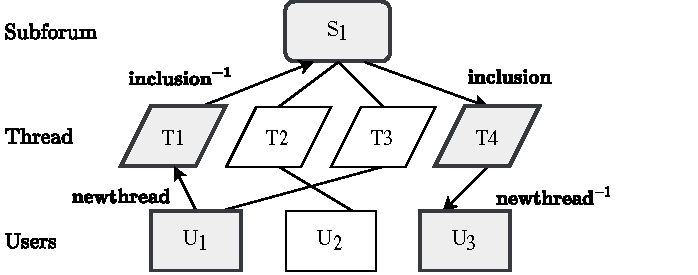
\includegraphics[width=\linewidth]{sysml/figures/metapathExample.pdf}
    \caption{An instance of meta-path ‘UTSTU’ in a subgraph of the forum graph.}
    \label{fig:metapath}
\end{figure}

\subsection{Episode Embedding}
The embeddings of each component of a post are concatenated into a $d_e = d_t + d_{\tau} + d_c$ dimensional embedding.
An episode with $L$ posts, therefore, has a $L \times d_e$ embeddings. 
We generate a final embedding for each episode, given the post embeddings using two different models.
In \textbf{Mean Pooling}, the episode embedding is the mean of $L$ post embeddings, resulting in a $d_e$ dimensional episode embedding.
For the \textbf{Transformer}, the episode embeddings are fed as the inputs to a transformer model~\cite{devlin2019bert,vaswani2017attention}, with each post embedding acting as one element in a sequence for a total sequence length $L$. 
We follow the architecture proposed by~\citet{andrews2019learning} and omit a detailed description of the transformer architecture for brevity (Figure~\ref{fig:emb_transformer} shows an overview).
Note that we do not use positional embeddings within this pooling architecture.
The parameters of the component-wise models and episode embedding models comprise the episode embedding $f_{\theta}: \left\{(t, \tau, c)\right\}^L \xrightarrow[]{} \mathbbm{R} ^ E$.

\begin{figure}
    \centering
    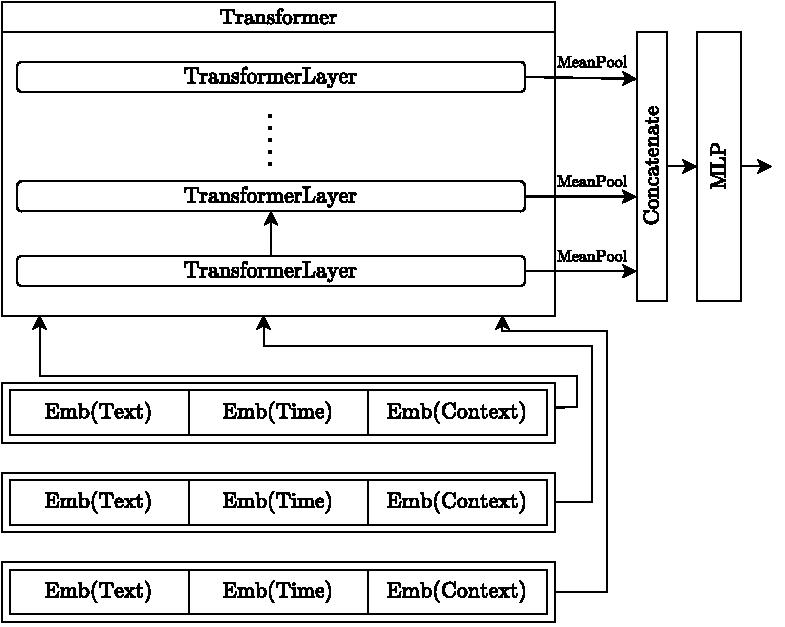
\includegraphics[width=0.7\linewidth]{sysml/figures/EmbeddingTransformer.pdf}
    \caption{Architecture for Transformer Pooling.
    %In mean pooling. The outputs from different layers are concatenated and then passed through an MLP to generate the final embedding for each episode.
    }
    \label{fig:emb_transformer}
\end{figure}

\subsection{Metric Learning}
\label{sec:framework:metric_learning}
An important element of our methodology is the ability to learn a distance function over user representations. We use the username as a label for the episode $e$ within the market $M$ and denote each username as a unique label $u \in U_M$.
Let $W =  |U_M| \times d_E $ represent a matrix denoting the weights corresponding to a specific metric learning method and let $x ^ * = \frac{x}{ || x||}$.
An example of a metric learning loss would be Softmax Margin, i.e., cross-entropy based softmax loss.
\begin{align*}
    P(u | e) = \frac{e^{W_{u} d_e}}{\sum\limits_{j=1}^{|U_M|}{e^{W_j d_e}}}
\end{align*}

We also explore alternative metric learning approaches such as Cosface (CF)~\cite{wang2018cosface}, ArcFace (AF)~\cite{deng2019arcface}, and MultiSimilarity (MS)~\cite{wang2019multi}. 

\subsection{Single-Task Learning}
The components discussed in the previous sections are combined together to generate  an embedding and the aforementioned tasks are used to train these models. 
Given an episode $e = \{(t_i, \tau_i, c_i) | 1 \leq i \leq L\}$, the componentwise embedding modules generate embedding for the text, time, and context, respectively.
The pooling module combines these embeddings into a single embedding $e \in \mathbbm{R}^E$. 
We define $f_\theta$ as the combination of the transformations that generate an embedding from an \textit{episode}.
Using a final metric learning loss corresponding to the task-specific $g_\phi$, we can train the parameters $\theta$ and $\phi$.
The framework, as defined in Figure~\ref{fig:main_workflow}, results in a model trainable for a single market $M_i$. 
Note that the first half of the framework (i.e., $f_\theta$) is sufficient to generate embeddings for episodes, making the module invariant to the choice of $g_\phi$. 
However, the embedding modules learned from these embeddings may not be compatible for comparisons across different markets, which motivates our multi-task setup. 

\subsection{Multi-Task Learning}

We use authorship attribution as the metric learning task for each market.
Further, a majority of the embedding modules are shared across the different markets.
Thus, in a multi-task setup, the model can share episode embedding weights (except context, which is market dependent) across markets. 
A shared BPE vocabulary allows weight sharing for text embedding on the different markets. 
However, the task-specific layers are not shared (different authors per dataset), and sharing $f_\theta$ does not guarantee alignment of embeddings across datasets (to reflect migrant authors). 
To remedy this, we construct a small, manually annotated set of labeled samples of authors known to have migrated from one market to another.
Additionally, we add pairs of authors known to be distinct across datasets.
The \textit{cross-dataset} consists of all episodes of authors that were manually annotated in this fashion.
The first step in the multi-task approach is to choose a market {($\mathcal{T}_M$)} or cross-market {($\mathcal{T}_{cr}$)} metric learning task $\mathcal{T}_i \sim \mathcal{T} =  \{\mathcal{T}_M, \mathcal{T}_{cr} \}$.
Following this, a batch of $N$ episodes $\mathcal{E} \sim \mathcal{T}_i$ is sampled from the corresponding task.
The embedding module generates the embedding for each episode $f_{\theta}^N: \mathcal{E} \xrightarrow[]{} \mathbbm{R}^{N \times E}$. 
Finally, the task-specific metric learning layer $g_{\phi}^{\mathcal{T}_i}$ is selected and a task-specific loss is backpropagated through the network. 
Note that in the \textit{cross-dataset}, new labels are defined based on whether different usernames correspond to the same author and episodes are sampled from the corresponding markets. 
Figure~\ref{fig:multitask_setup} demonstrates the shared layers and the use of \textit{cross-dataset} samples. 
The overall loss function is the sum of the losses across the markets: $\mathcal{L} = \underset{\mathcal{T}_i \sim \mathcal{T},\ \mathcal{E} \sim \mathcal{T}_i}{\mathbbm{E}}\left[\mathcal{L}_i(\mathcal{E})\right] $.
\begin{figure}
    \centering
    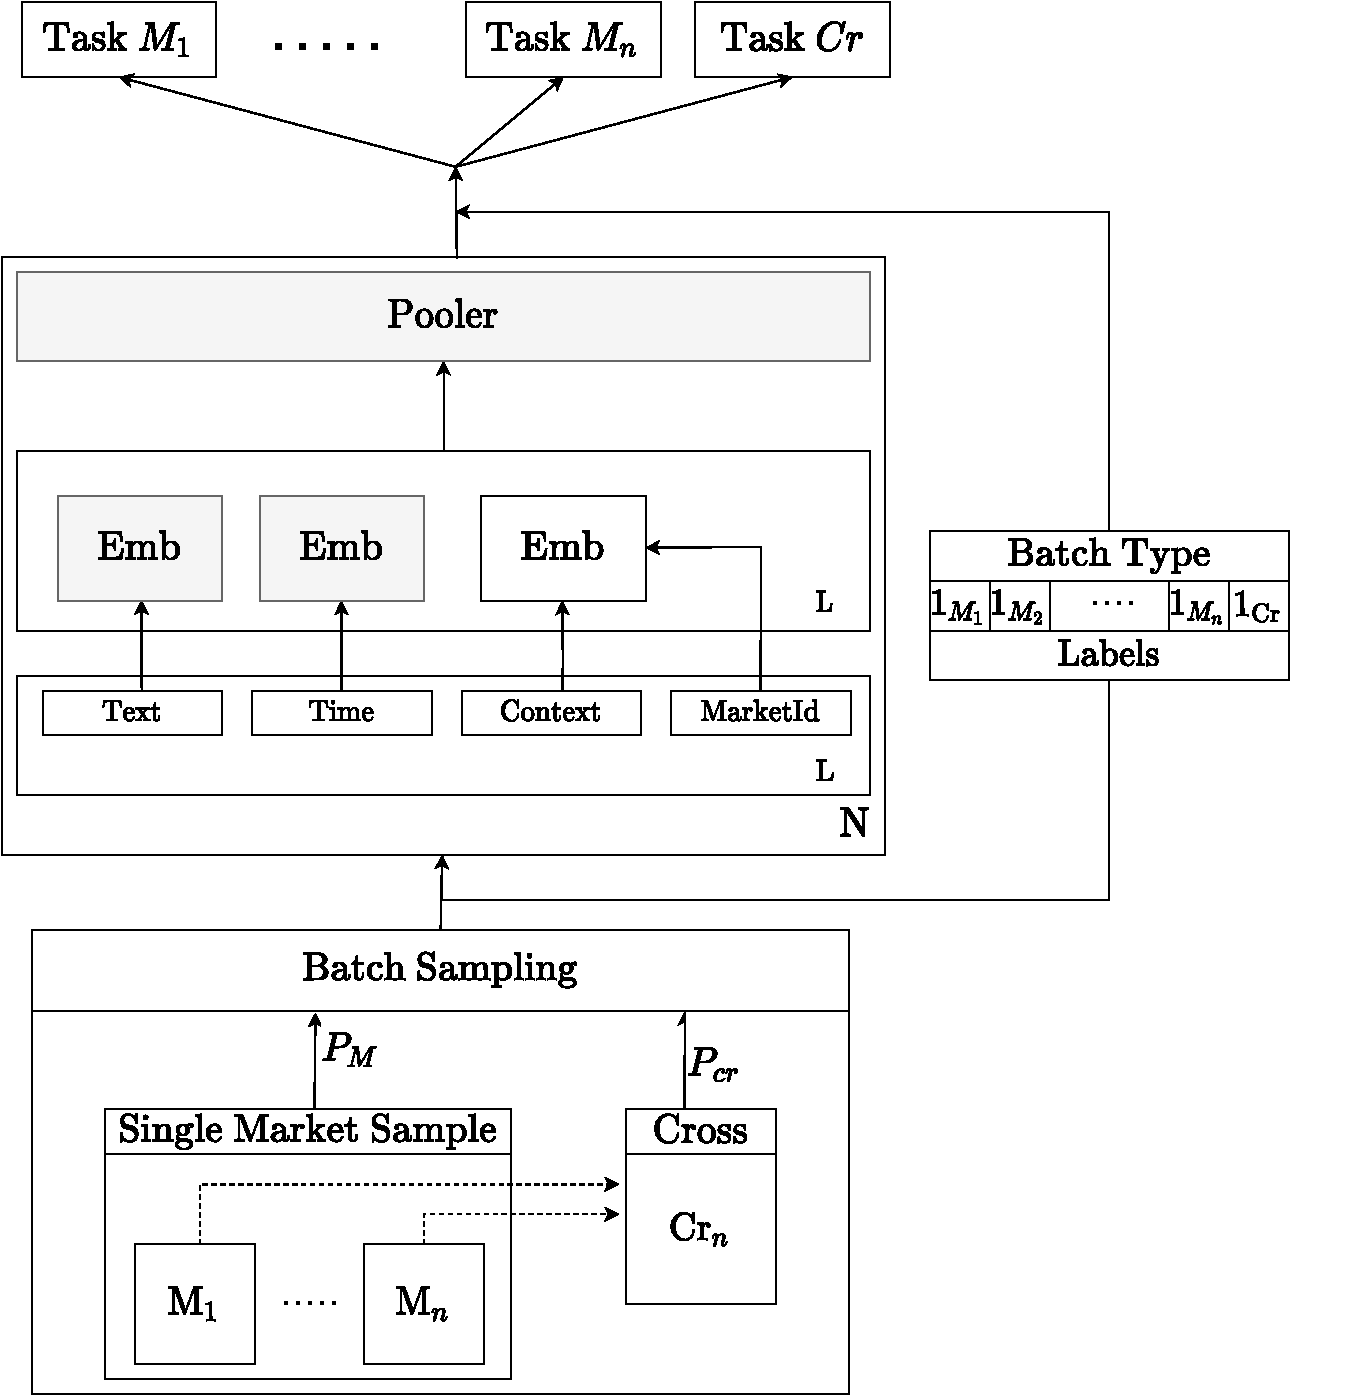
\includegraphics[width=0.8\linewidth]{sysml/figures/MultiTask.pdf}
    \caption{Multi-task setup. Shaded nodes are shared}
    \label{fig:multitask_setup}
\end{figure}



\section{Evaluation}
\label{sec:sysml:eval}
While ground truth labels for a single author having multiple accounts are unavailable, individual models can still be compared by measuring their performance on authorship attribution as a proxy. 
%We compare these approaches using a retrieval based setup over the generated output embeddings which reflects the clustering of episodes for each author.
We evaluated our method using retrieval-based metrics over the embeddings generated by each approach. % where embeddings corresponding to each approach are generated, and a random subset of the episode embeddings is sampled.
Denote the set of all episode embeddings as $E = \{e_1, \dots e_n\}$ and let $Q = \{q_1, q_2, \dots q_\kappa\} \subset E$ be the sampled subset.
We computed the cosine similarity of the query episode embeddings with all episodes. Let $R_i = \langle r_{i1}, r_{i2}, \dots r_{in} \rangle$ denote the list of episodes in $E$ ordered by their cosine similarity with episode $q_i$ (excluding itself) and let $A(.)$ map an episode to its author. The following measures are computed.

\noindent \textbf{Mean Reciprocal Rank}: (MRR) The RR for an episode is the reciprocal rank of the first element (by similarity) with the same author. MRR is the mean of reciprocal ranks for a sample of episodes.
\begin{align*}
    MRR(Q) = \frac{1}{\kappa}\sum_{i=1}^\kappa \frac{1}{\min\limits_j  \left(A(r_{ij}) = A(e_i)\right)}
\end{align*}
%where $\tau_i = \min\limits_j  \left(A(r_{ij}) = A(e_i)\right)$ is the rank of the nearest episode by the same author.

\noindent \textbf{Recall@k}:  (R@k)  Following~\citet{andrews2019learning}, we define the R@k for an episode $e_i$ to be an indicator denoting whether an episode by the same author occurs within the subset $ \langle r_{i1}, \dots, r_{ik} \rangle$. R@k denotes the mean of these recall values over all the query samples.

\begin{align*}
    R@k = \frac{1}{\kappa}\sum\limits_{i=1}^{\kappa}{\1_{\{\exists\ j | 1 \leq j \leq k, A(r_{ij}) = A(e_i)\}}}
\end{align*}

\noindent \textbf{Baselines}
We compare our best model against two baselines. First, we consider a popular short text authorship attribution model~\cite{shrestha2017convolutional} based on embedding each post using character CNNs. 
While the method had no support for additional attributes (time, context) and only considers a single post at a time, we compare variants that incorporate these features as well. 
The second method for comparison is invariant representation of users~\cite{andrews2019learning}. This method considers only one dataset at a time and does not account for graph-based context information. 
Results for episodes of length 5 are shown in Table~\ref{tab:baselines_comparison}

%\noindent \textbf{Hyperparameters}

\begin{table*}
    \centering
    \resizebox*{\linewidth}{!}{
		\begin{tabular}{lcccccccc}
 		\toprule
			\multirow{2}{*}{Method}	&\multicolumn{2}{c}{BMR}	&	\multicolumn{2}{c}{Agora}	&	\multicolumn{2}{c}{SR2}	&	\multicolumn{2}{c}{SR}\\
					&MRR&	R@10&	MRR&	R@10&	MRR&	R@10&	MRR&	R@10\\
		\midrule
			\citet{shrestha2017convolutional} (CNN) &	0.07	&	0.165	&	0.126	&	0.214	&	0.082	&	0.131	&	0.036	&	0.073	\\
			 + time + context &	0.235	&	0.413	&	0.152	&	0.263	&	0.118	&	0.21	&	0.094	&	0.178	\\
			 + time + context + transformer pooling &	0.219	&	0.409	&	0.146	&	0.266	&	0.117	&	0.207	&	0.113	&	0.205	\\
		\hline
			\citet{andrews2019learning} (IUR) \\
			 mean pooling &	0.223	&	0.408	&	0.114	&	0.218	&	0.126	&	0.223	&	0.109	&	0.19	\\
			 transformer pooling&	0.283	&	0.477	&	0.127	&	0.234	&	\textit{0.13}	&	\textit{0.229}	&	0.118	&	0.204	\\
		\hline
			\SYSMLmethodname{} (single) &	\textit{0.32}	&	\textit{0.533}	&	\textit{0.152}	&	\textit{0.279}	&	0.123	&	0.21	&	\textit{0.157}	&	\textit{0.266}	\\
			 - graph context &	0.265	&	0.454	&	0.144	&	0.251	&	0.089	&	0.15	&	0.049	&	0.094	\\
			 -graph context - time &	0.277	&	0.477	&	0.123	&	0.198	&	0.079	&	0.131	&	0.04	&	0.08	\\
		\hline
			\SYSMLmethodname{}  (multitask) &	\textbf{0.438}	&	\textbf{0.642}	&	\textbf{0.303}	&	\textbf{0.466}	&	\textbf{0.304}	&	\textbf{0.464}	&	\textbf{0.227}	&	\textbf{0.363}	\\
			 - graph context &	0.396	&	0.602	&	\textbf{0.308}	&	\textbf{0.469}	&	0.293	&	0.442	&	0.214	&	0.347	\\
			 - graph context - time &	0.366	&	0.575	&	0.251	&	0.364	&	0.236	&	0.358	&	0.167	&	0.28	\\
		\bottomrule
	\end{tabular}
    }
    \caption{Best performing results in {\bf bold}. Best performing single-task results in {\it italics}. All  $\sigma_{MRR}< 0.02$, $\sigma_{R@10} < 0.03$, For all metrics, higher is better. Results suggest single-task performance largely outperforms the state-of-the-art \cite{shrestha2017convolutional,andrews2019learning},
    while our novel multi-task cross-market setup offers a substantive lift ({\bf up to 2.5X on MRR and 2X on R@10}) over single-task performance.}
    \label{tab:baselines_comparison}
\end{table*}





\section{Analysis}
\label{sec:sysml:analysis}

\subsection{Model and Task Variations}
\begin{comment}
\begin{figure*}[!!htbp]
    \begin{subfigure}{0.5\textwidth}
        \centering
        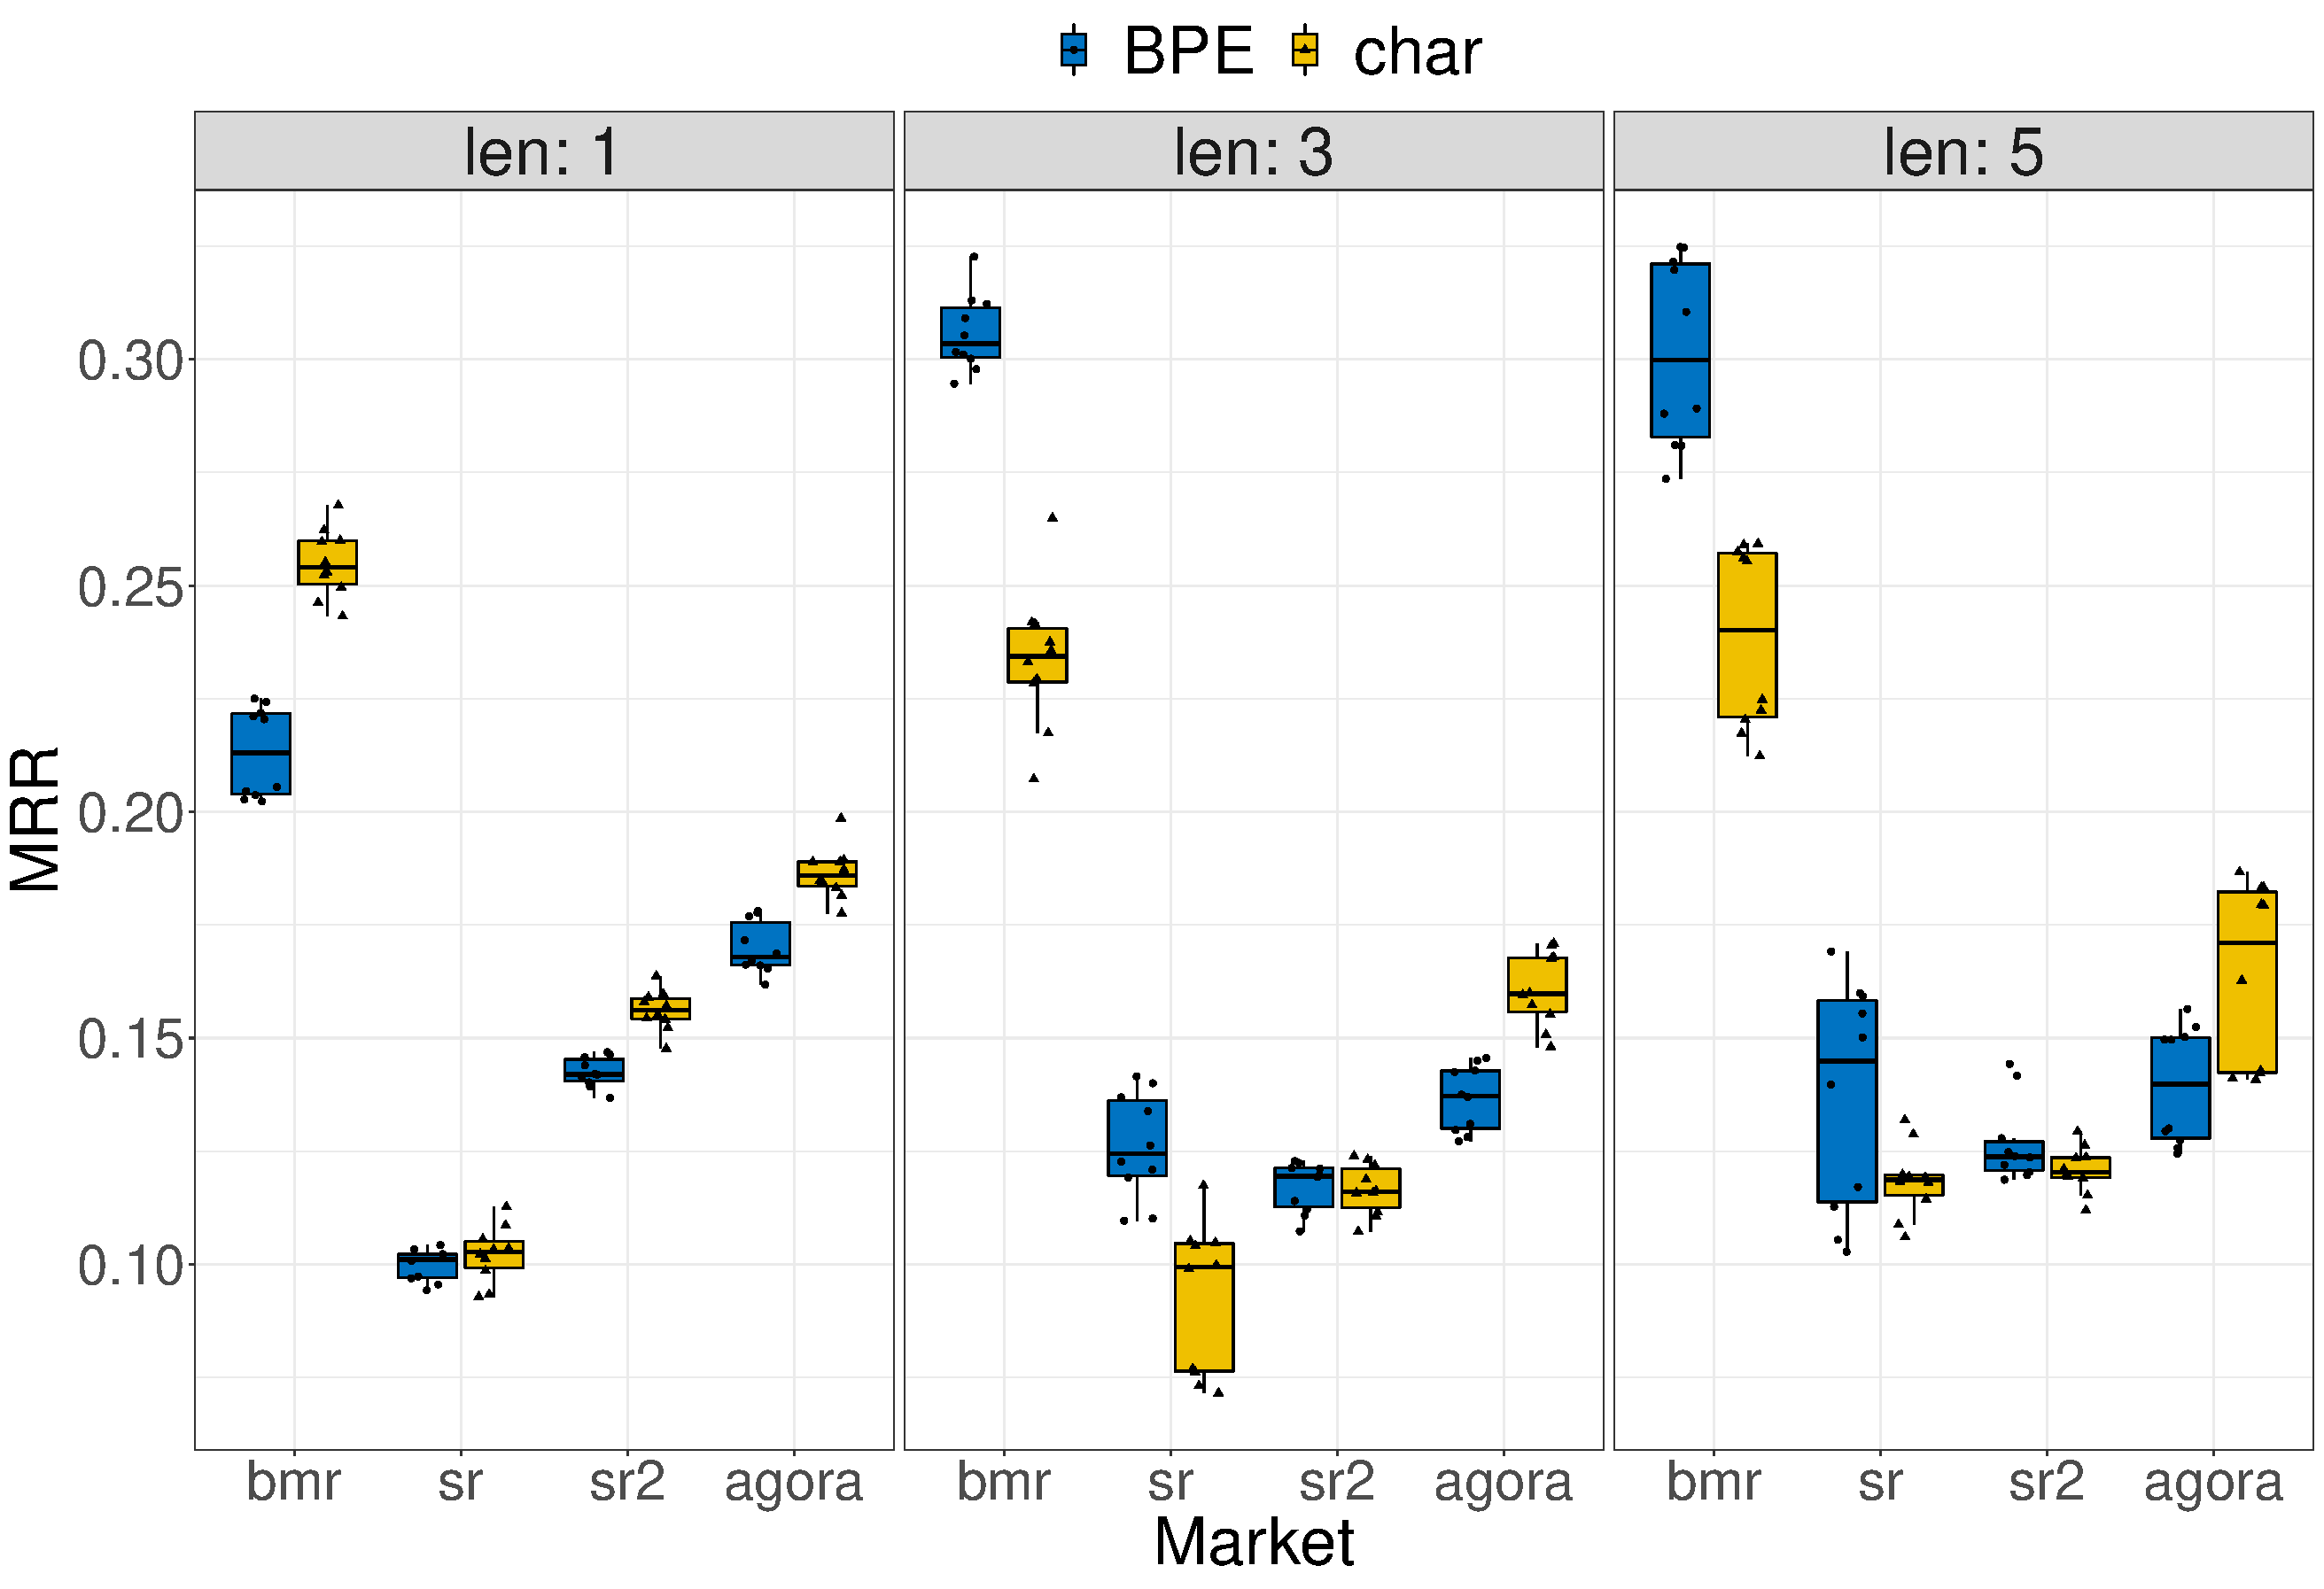
\includegraphics[width=\linewidth]{plots/tokenizer_comparison.pdf}
        \caption{Tokenizer}
        \label{fig:model_comp:tok}
    \end{subfigure} %
    \begin{subfigure}{0.5\textwidth}
        \centering
        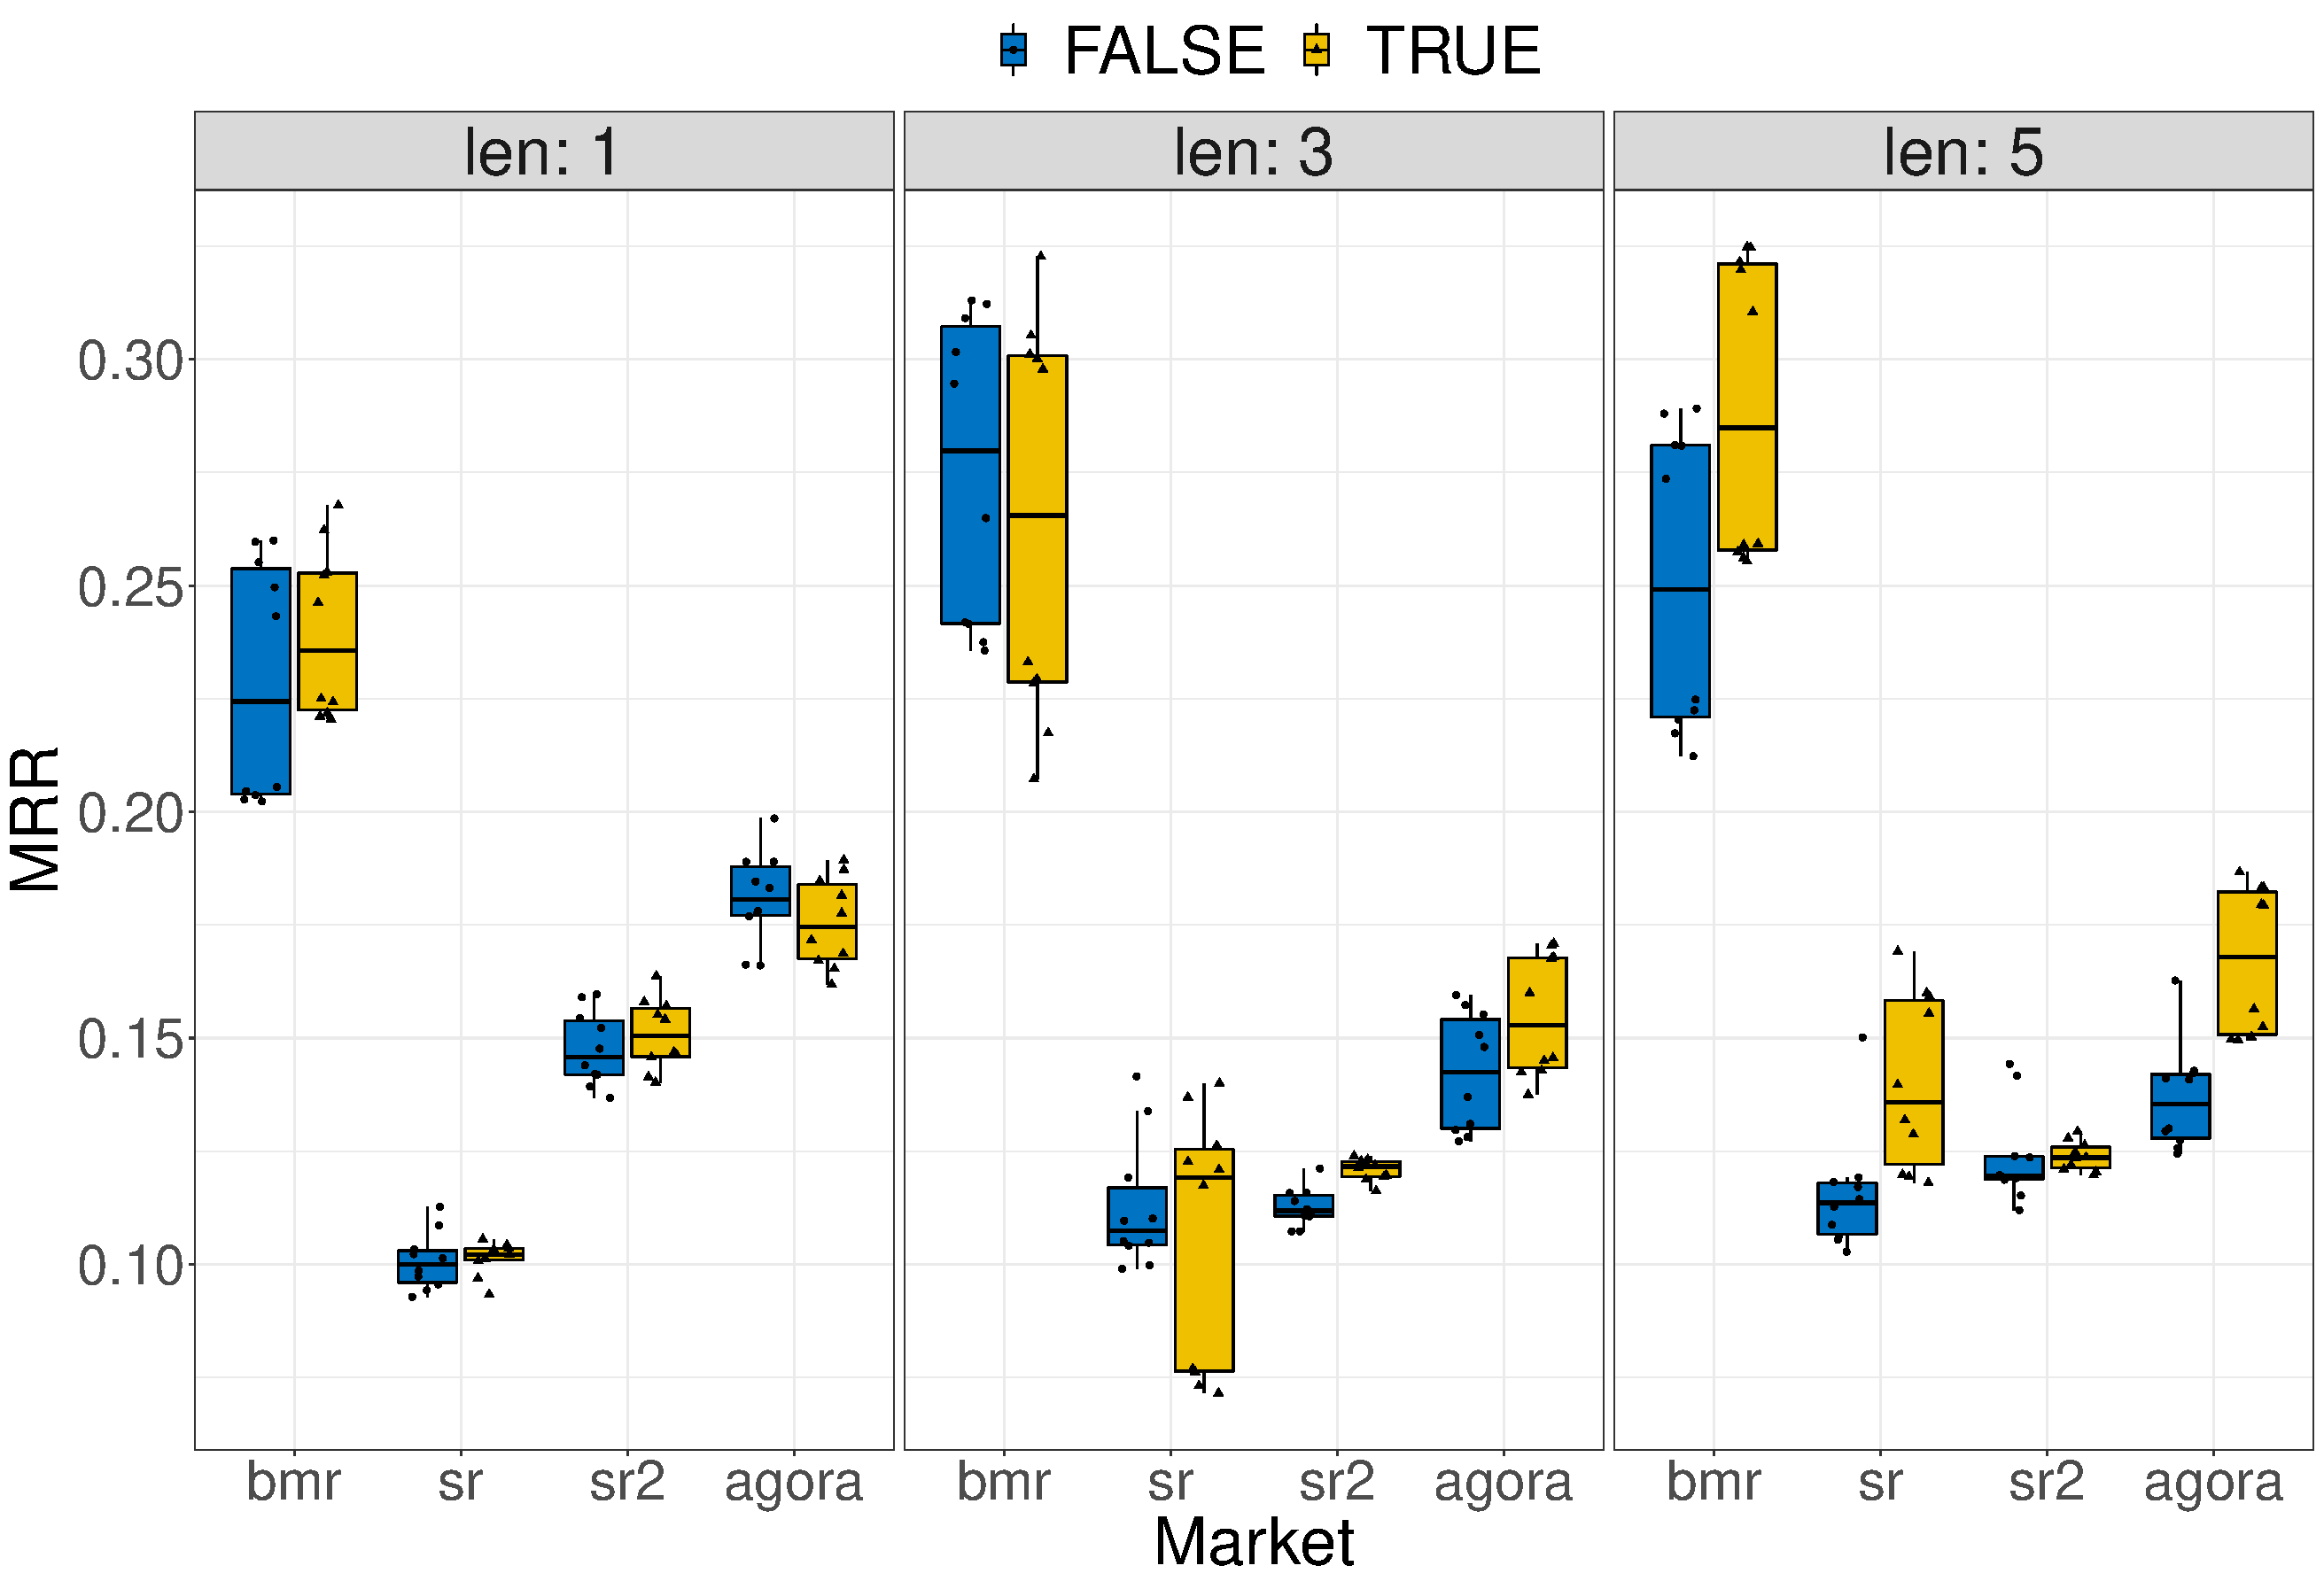
\includegraphics[width=\linewidth]{plots/graphemb_comparison.pdf}
        \caption{Graph Embedding}
        \label{fig:model_comp:graph}
    \end{subfigure} %
    \caption{Comparison of models across Tokenizer variants (top) and usage of graph embedding (bottom). TRUE/FALSE refer to whether the model is initialized with pretrained HIN context embeddings. \textcolor{blue}{SP: Is this figure particularly useful -- does it add to the accompanying text you have laid out w.r.t WMW test?}}
    \label{fig:model_comp}
\end{figure*}\textcolor{red}{replace Figure~\ref{fig:model_comp} with table}
\end{comment}
%Figure~\ref{fig:model_comp} demonstrates two of the modeling decisions - the choice of tokenizer and the impact of using pretrained graph embeddings.
%\noindent \textbf{Single Task Model} 
To compare the variants using statistical tests, we compute the MRR of the data grouped by market, episode length, tokenizer, and a graph embedding indicator.
This leaves a small number of samples for paired comparison between groups, which precludes making normality assumptions for a t-test. 
Instead, we applied the paired two-samples Wilcoxon-Mann-Whitney (WMW) test~\cite{mann1947test}.
The first key contribution of our model is the use of meta-graph embeddings for context. 
The WMW test demonstrates that using pretrained graph embeddings was significantly better than using random embeddings ($p < 0.01$). 
Table~\ref{tab:baselines_comparison} shows a summary of these results using ablations.
For completeness of the analysis, we also compare the character and BPE tokenizers.
WMW failed to find any significant differences between the BPE and character models for embedding (table omitted for brevity). 
Many darkweb markets tend to have more than one language (e.g., BMR had a large German community), and BPE  allows a shared vocabulary to be used across multiple datasets with very few out-of-vocab tokens. 
Thus, we use BPE tokens for the forthcoming multitask models.
\begin{figure}[!htbp]
    \centering
    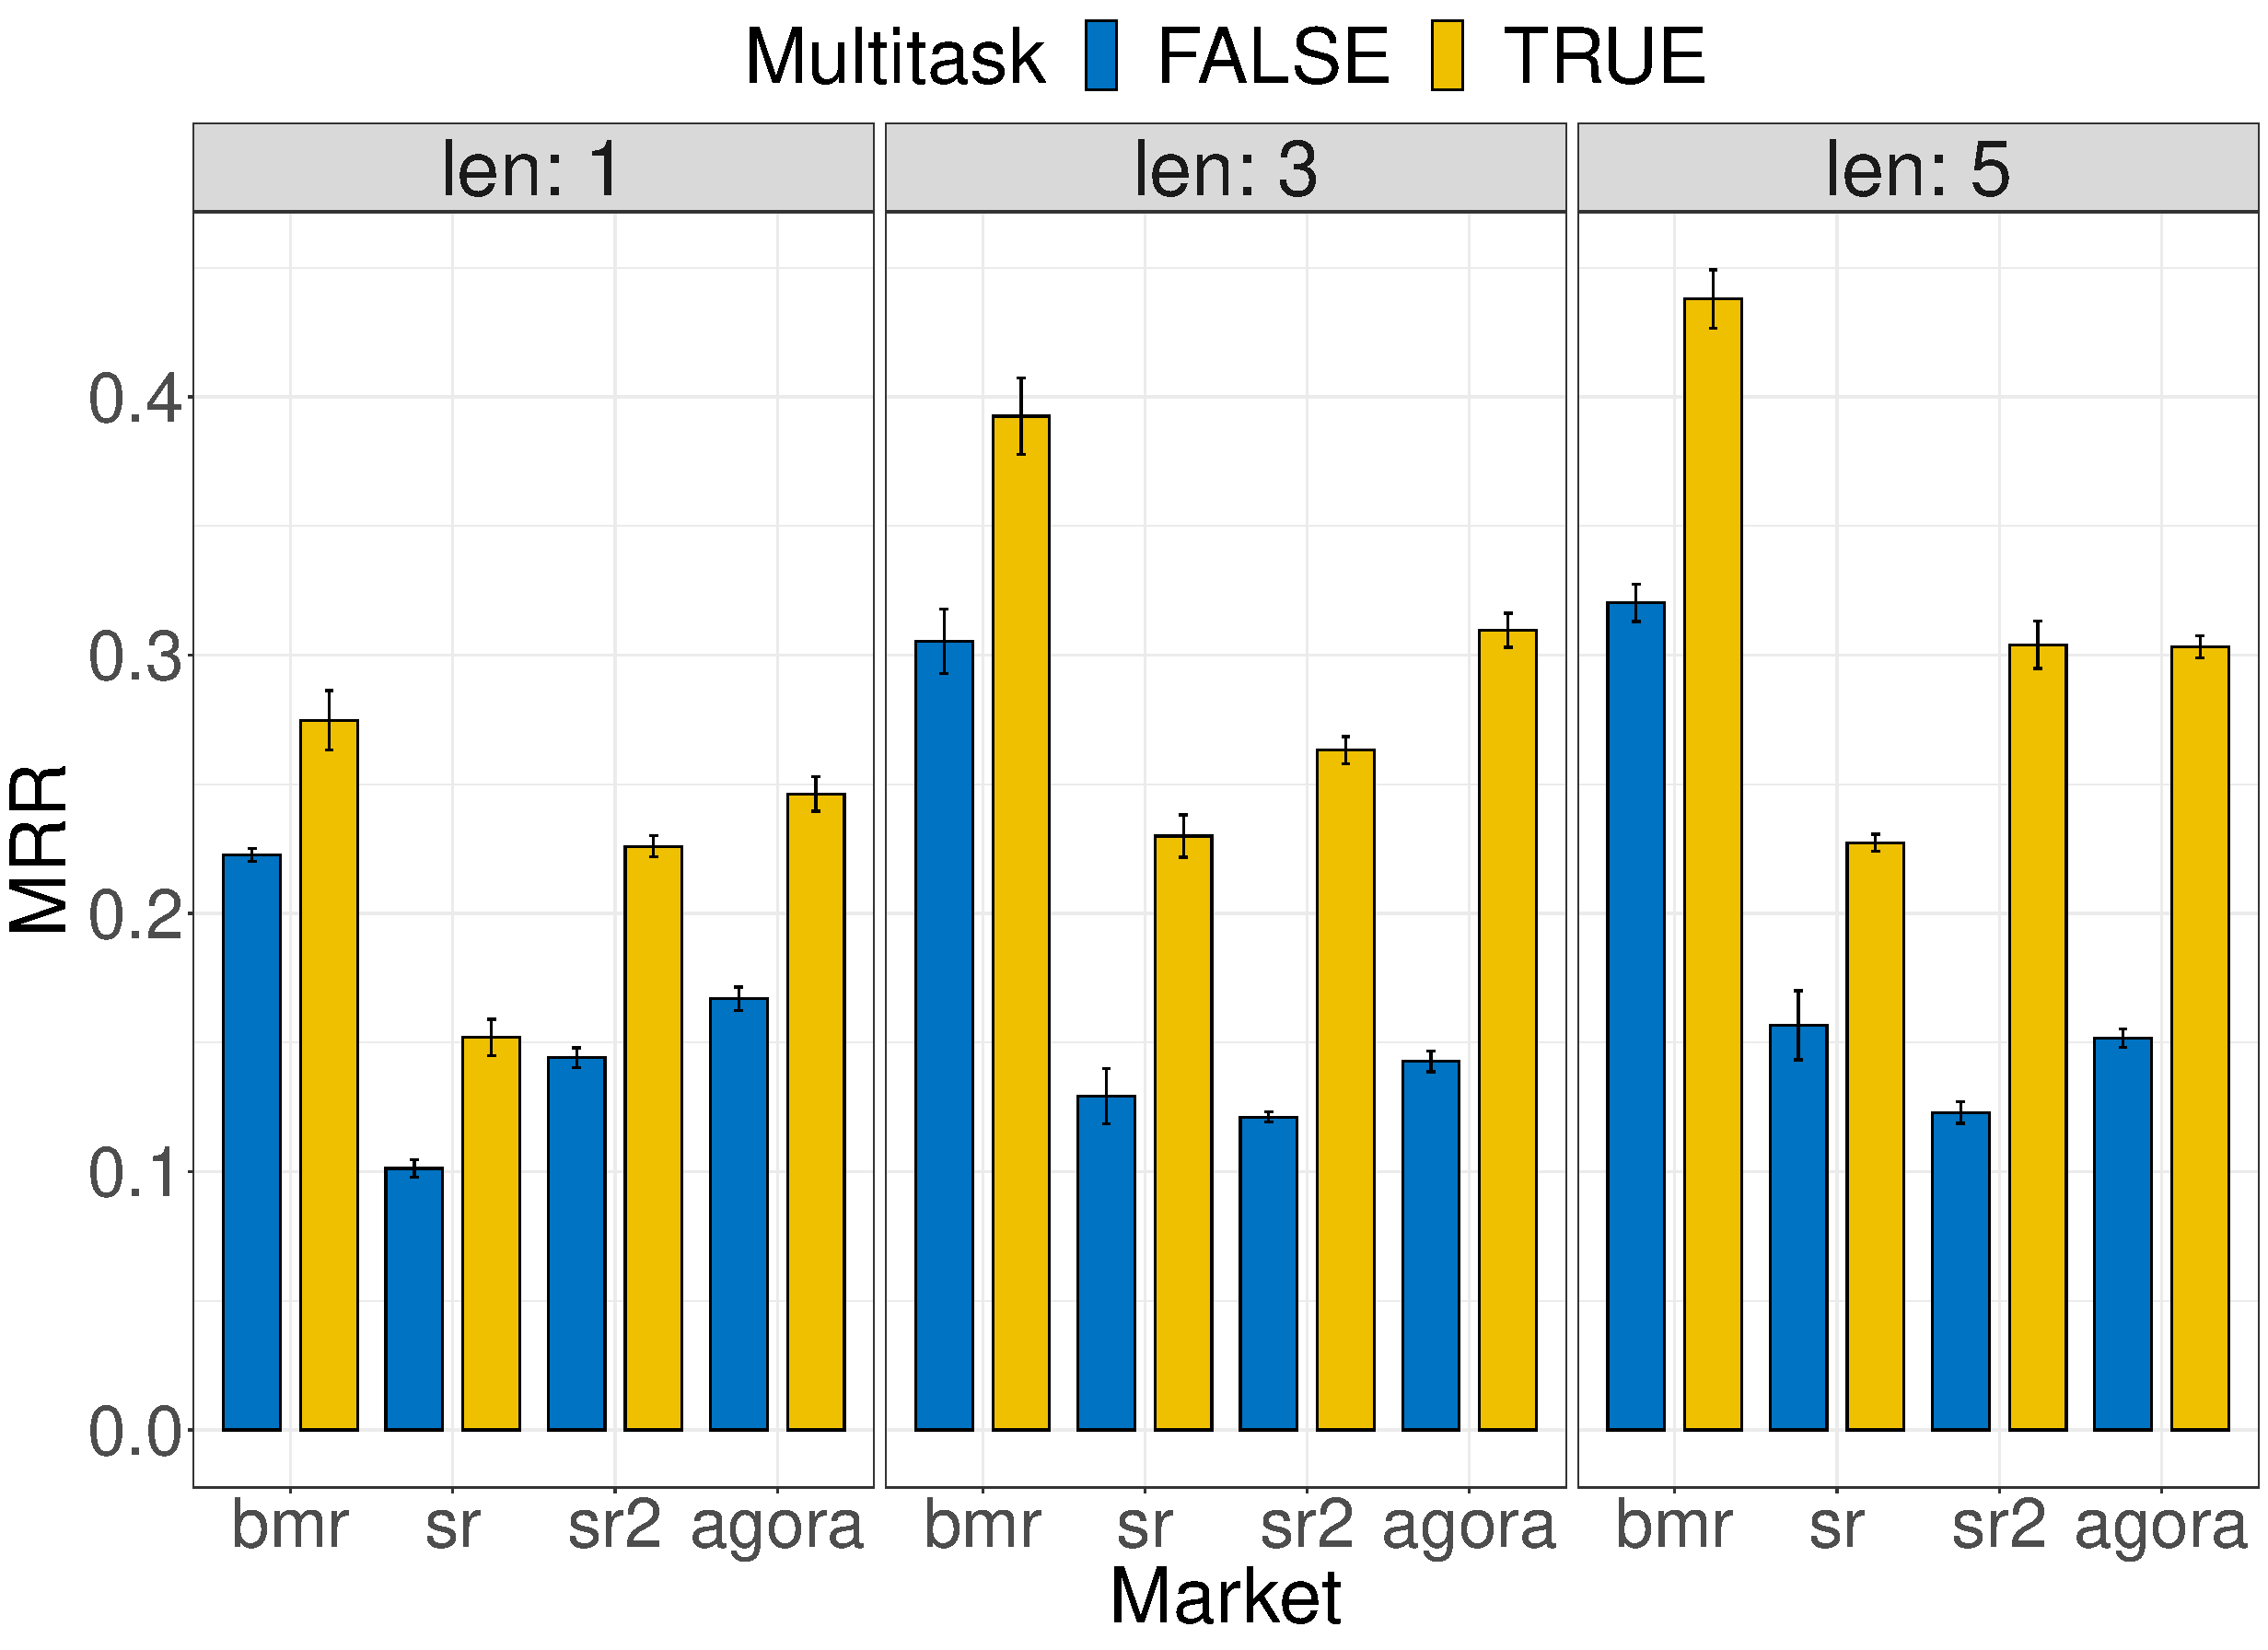
\includegraphics[width=0.8\linewidth,alt={Bar chart showing drill-down: one-at-a-time vs. multitask.}]{sysml/plots/multitask.pdf}
    \caption{Drill-down: one-at-a-time vs. multitask.}
    \label{fig:multitask_results}
\end{figure} 

\noindent \textbf{Multitask} Our second key contribution is the multitask setup.
Table~\ref{tab:baselines_comparison} demonstrates that \SYSMLmethodname{} (multitask) outperforms all baselines on episodes of length 5. We further compare runs of the best single task model for each market against a multitask model. %trained with $P(\text{cross\_sampling}) = 0.01$. 
Figure~\ref{fig:multitask_results} demonstrates that multitask learning  consistently and significantly (WMW: $p < 0.01$) improves performance across all markets and all episode lengths. 




\noindent \textbf{Metric Learning}
Recent benchmark evaluations have demonstrated that different metric learning methods provide only marginal improvements over classification~\cite{musgrave2020metric,Zhai2019ClassificationIA}. 
We experimented with various state-of-the-art metric learning methods (\S\ref{sec:framework:metric_learning}) in the multi task setup and found that softmax-based classification (SM) was the best performing method in 3 of 4 cases for episodes of length 5 (Figure~\ref{fig:metric_learning}). 
Across all lengths, SM is significantly better (WMW: $p < 1e-8$) and therefore we use SM in \SYSMLmethodname{}.

\begin{figure}[!htbp]
    \centering
    \includegraphics[width=0.8\linewidth,alt={Bar chart showing comparison of metric learning approaches.}]{sysml/plots/nce_comparison_multitask.pdf}
    \caption{Task comparison: SM and CF are better performing two methods, with SM better in 3 of 4 cases.}
    \label{fig:metric_learning}
\end{figure}
%\textcolor{red}{Consider dropping to single line}
%Recent benchmark evaluations have demonstrated that different metric learning methods provide only marginal improvements over classification~\cite{musgrave2020metric,Zhai2019ClassificationIA}. 
%We experimented with various state-of-the-art metric learning methods (\S\ref{sec:framework:metric_learning}) in the multi task setup and found that softmax-based classification (SM) was significantly better (WMW: $p < 0.01$). Therefore, we use SM in \SYSMLmethodname{}. 
%For additional details see the appendix.


\begin{comment}
\begin{figure}[!htbp]
    \centering
    \includegraphics[width=0.7\linewidth]{plots/nce_comparison_multitask.pdf}
    \caption{Task comparison: SM and CF are better performing two methods, with SM better in 3 of 4 cases.}
    \label{fig:metric_learning}
\end{figure}
\end{comment}

\begin{comment}
\noindent \textbf{Episode Length}  Figure~\ref{fig:len_comparison} shows a comparison of the mean performance of each model across various episode lengths. We see that compared to the baselines, \SYSMLmethodname{} can combine contextual and stylistic information across multiple posts more effectively. 

\begin{figure}[!htbp]
    \centering
    \includegraphics[width=0.7\linewidth]{plots/length_comparison.pdf}
    \caption{\SYSMLmethodname{} is more effective at utilizing multi post stylometric informatio.n}
    \label{fig:len_comparison}
\end{figure}
\end{comment}


\subsection{Novel Users}
The dataset statistics (Table~\ref{tab:dataset_stats}) indicate that there are users in each dataset who have no posts in the time period corresponding to the training data. 
To understand the distribution of performance across these two configurations, we compute the test metrics over two samples.
For one sample, we constrain the sampled episodes to those by users who have at least one episode in the training period (Seen Users).
For the second sample, we sample episodes from the complement of the episodes that satisfy the previous constraint (Novel Users).
Figure~\ref{fig:novel_vs_train_comparison} shows the comparison of MRR on these two samples against the best single task model for episodes of length 5. 
Unsurprisingly, the first sample (Seen Users) have better query metrics than the second (Novel Users).
However, importantly both of these groups outperformed the best single task model results on the first group (Seen Users), which demonstrates that the {\it lift offered by the multitask setup is spread across all users.} 

\begin{figure}
    \centering
    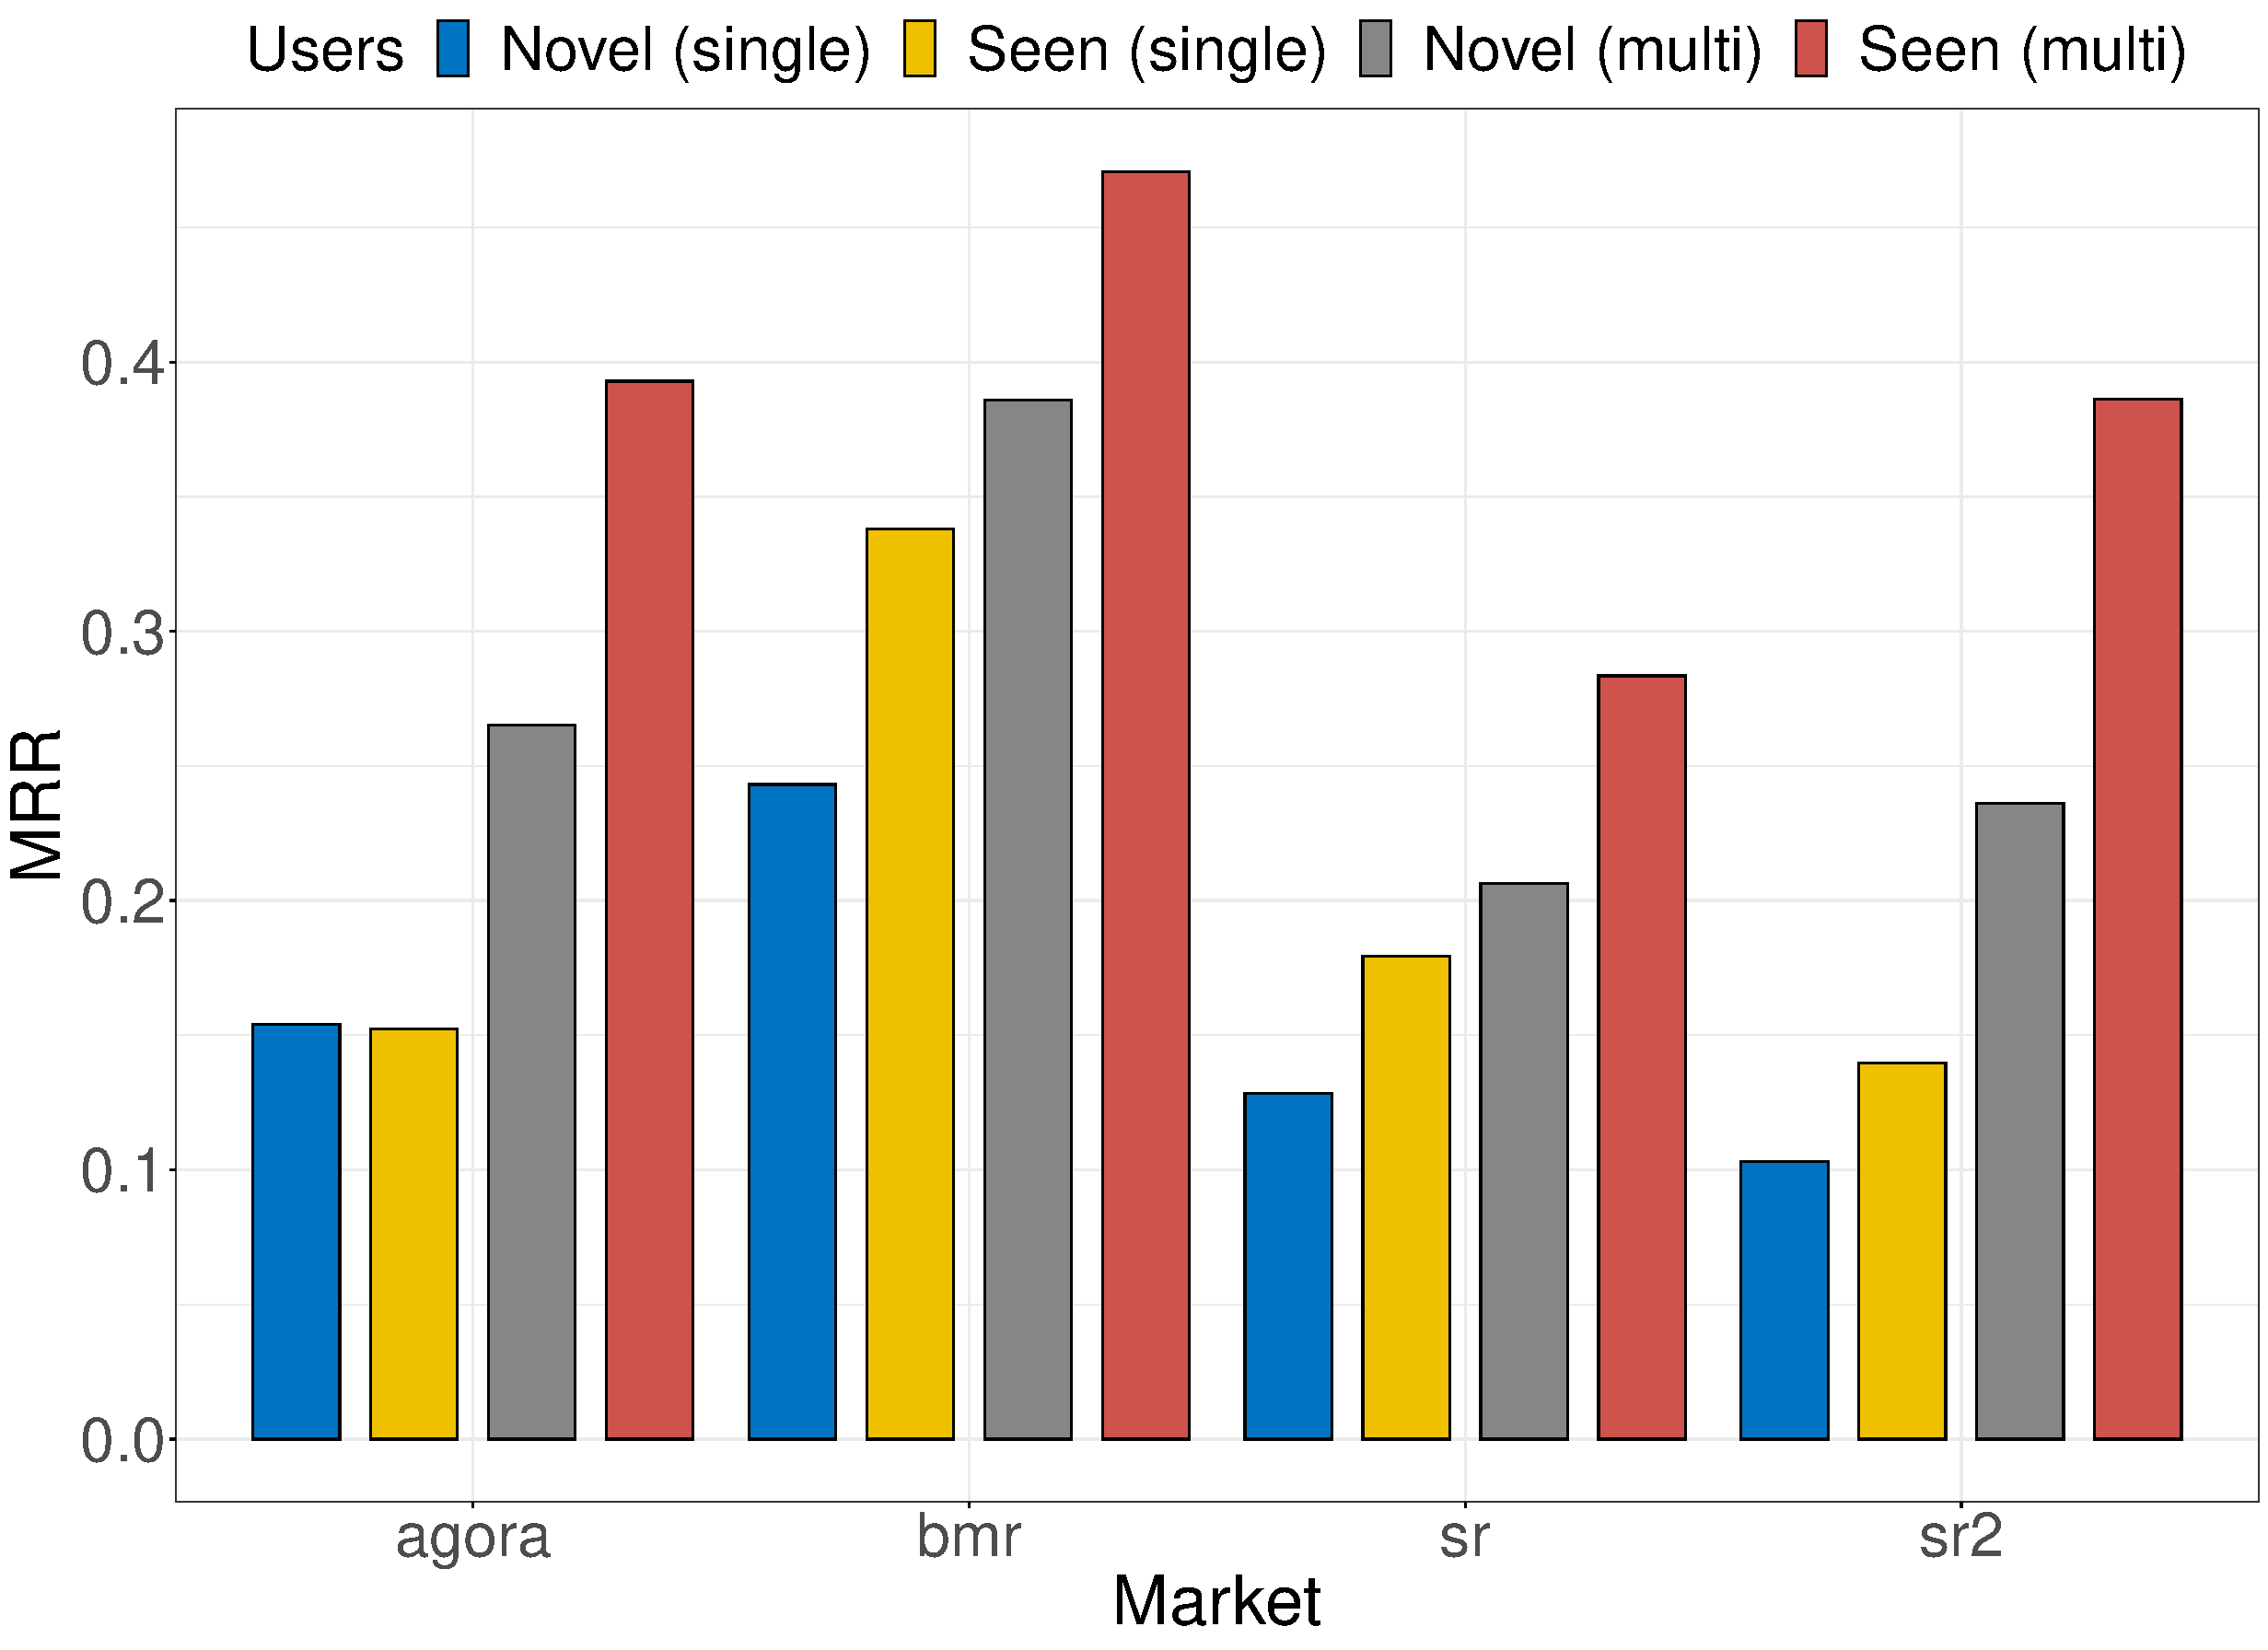
\includegraphics[width=0.8\linewidth,alt={Bar chart showing the lift provided by using the multitask setup across both seen and novel users.}]{sysml/plots/novel_vs_train_vs_single.pdf}
    \caption{Lift on the multitask setup across users.}
    \label{fig:novel_vs_train_comparison}
\end{figure}

\noindent \textbf{Episode Length}  Figure~\ref{fig:len_comparison} shows a comparison of the mean performance of each model across various episode lengths. We see that compared to the baselines, \SYSMLmethodname{} can combine contextual and stylistic information across multiple posts more effectively. Additional results (see appendix),  indicate that this trend continues for larger episode sizes.

\begin{figure}[!htbp]
    \centering
    \includegraphics[width=0.8\linewidth,alt={Line chart showing the improvements from \SYSMLmethodname{} across different episode lengths.}]{sysml/plots/length_comparison.pdf}
    \caption{\SYSMLmethodname{} is more effective at utilizing multi post stylometric information}
    \label{fig:len_comparison}
\end{figure}


\begin{figure}
    \centering
    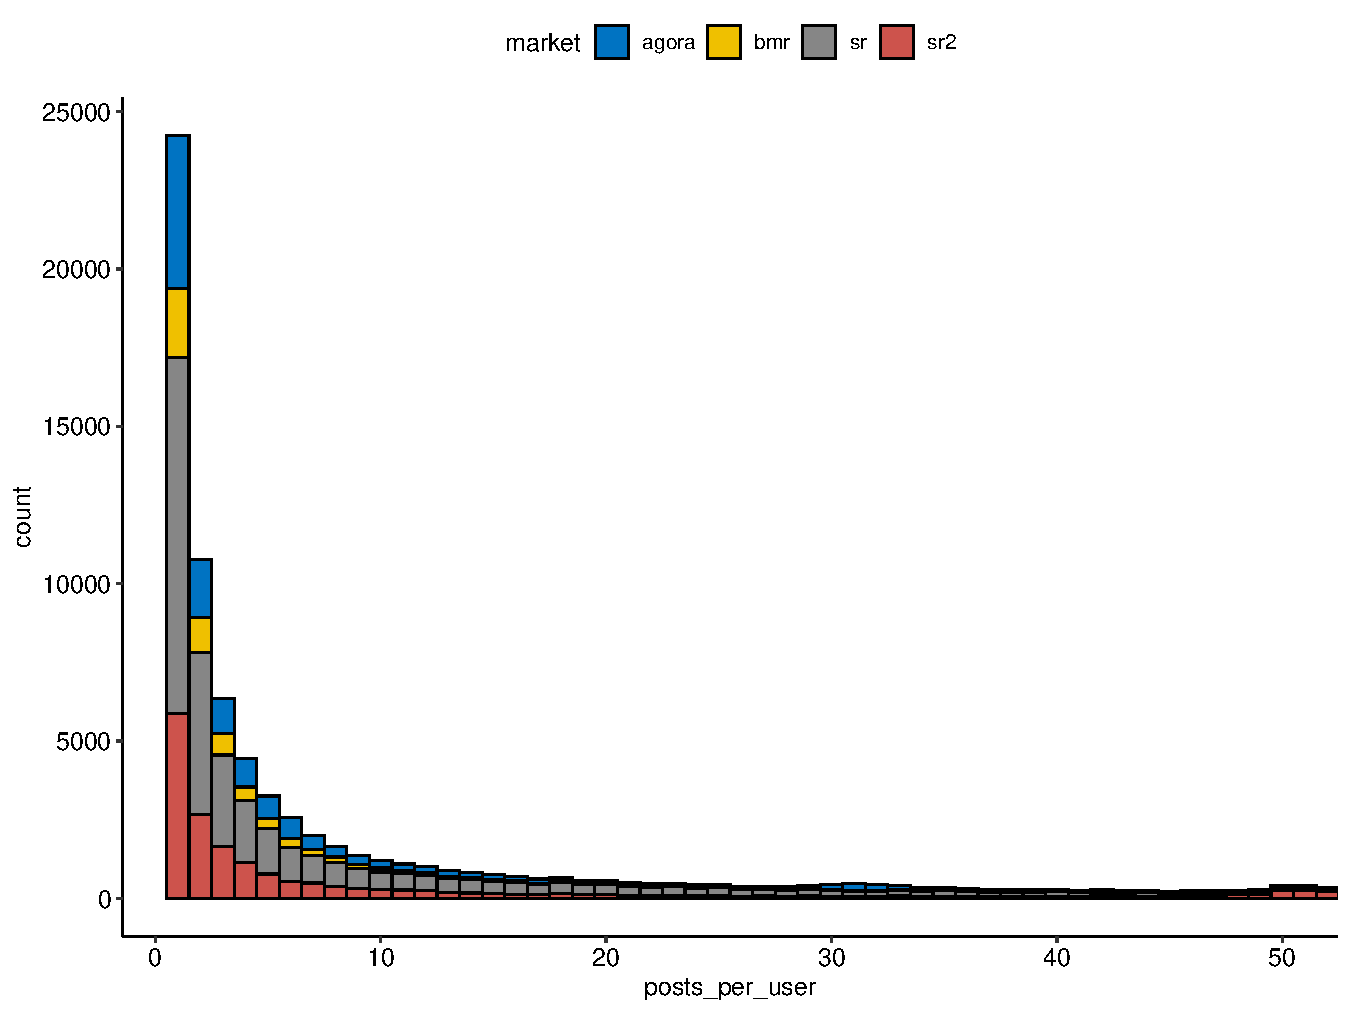
\includegraphics[width=\linewidth,alt={Histogram of posts per user.}]{sysml/plots/posts_histogram.pdf}
    \caption{Frequency of number of posts per user}
    \label{fig:posts_freq}
\end{figure}

\begin{table*}[!htbp]
    \small
    \centering
		\begin{tabular}{lcccccccc}
 		\toprule
			\multirow{2}{*}{Method}	&\multicolumn{2}{c}{BMR}	&	\multicolumn{2}{c}{Agora}	&	\multicolumn{2}{c}{SR2}	&	\multicolumn{2}{c}{SR}\\
					&MRR&	R@10&	MRR&	R@10&	MRR&	R@10&	MRR&	R@10\\
		\midrule
			\SYSMLmethodname{}  (singletask) &	0.305	&	0.508	&	0.186	&	0.32	&	0.159	&	0.273	&	0.14	&	0.246	\\
				\hline
			\SYSMLmethodname{}  (multitask) &	0.484	& 0.689	&	0.349	&	0.519	&	0.401	&	0.556	&	0.292	&	0.429	\\
					\bottomrule
    	\end{tabular}
    	\caption{Additional results for 7 posts per episode}
      \label{tab:additional_res_7}
\end{table*}

\begin{table*}[!htbp]
    \small
    \centering
		\begin{tabular}{lcccccccc}
 		\toprule
			\multirow{2}{*}{Method}	&\multicolumn{2}{c}{BMR}	&	\multicolumn{2}{c}{Agora}	&	\multicolumn{2}{c}{SR2}	&	\multicolumn{2}{c}{SR}\\
					&MRR&	R@10&	MRR&	R@10&	MRR&	R@10&	MRR&	R@10\\
		\midrule
			\SYSMLmethodname{}  (singletask) &	0.264 & 0.48	&	0.146	&	0.249	&	0.165   &	0.272	&	0.194	&	0.319	\\
				\hline
			\SYSMLmethodname{}  (multitask) &	0.4667	&	 0.648	&	0.357	&	0.498	&	0.377	&	0.522	&	0.299	&	0.449	\\
					\bottomrule
    	\end{tabular}
    	\caption{Additional results for 9 posts per episode}
      \label{tab:additional_res_9}
\end{table*}

From Figure~\ref{fig:posts_freq}, we see that the number of users reduces rapidly as the posts per user decrease. Thus, we limited our analysis to up to 5 posts per episode.
For completeness, we also provide additional results for 7 and 9 posts per episode in Table~\ref{tab:additional_res_7} and ~\ref{tab:additional_res_9} respectively. Note that the histogram has some non-smooth bumps at around 10, 50, 100 posts as they act as the minimum number of posts for different levels of forum users. As explained in a previous section, users post on `newbie' forums until they reach a specific number of posts, leading to these unusual bumps in the histogram. 
We note that the performance of our methods continues to improve as the posts per episode are increased (at a cost to coverage - number of users studied), though the improvement is higher in the bigger markets as these tend to have a sufficiently large number of individuals with a higher number of total posts.


\section{Case Study}
\subsection{Qualitative Analysis of Attribution:}
\label{sec:sysml:casestudy:qualitative}
%The datasets consist of a varying distribution of episodes per author as well as variance in the ability to characterize of each author from their style. 
%For the remainder of 
In this section, we consider the average (euclidean) distance between each pair of episodes by the same author as a heuristic for stylometric identifiability (SI), where lower average distance corresponds to higher SI and vice versa. 
Somewhat surprisingly, 
%we found that the number of episodes for each author is not correlated with the stylometric identifiability (SI). 
authors with a small number of total episodes ($<10$) were found at both extremes of identifiability, while the authors with the highest number of episodes were in the intermediate regions, suggesting that SI is not strongly correlated with episode length.  Next, we further investigate these groups.
%We next drill down on this further.
%In this subsection, we supplement the aforementioned metric-based comparisons from \S\ref{sec:analysis} with a qualitative characterization of these extremes.

\noindent \textbf{High SI authors:} 
Among the 20 users with the lowest average distance between episodes, a single pattern is prominent. 
This first group of high SI users are "newbie" users.  On a majority of analyzed forums, a minimum number of posts by a user is required before posting restrictions are removed from the user's account.
Thus, users create threads on `Newbie Discussion' subforums.
Typical posts on these threads include repeated posting of the same message or numbered posts counting up to the minimum required. 
As users tend to make all these posts within a fixed time frame, the combination of repeated, similar stylistic text and time makes the posts easy to identify. 
Exemplar episodes from this "newbie" group are shown in Table~\ref{tab:example_posts}. 
%Note that the writing style of an author may not be captured by such posts, but there exist accounts with posts only in these threads, therefore there is no other way to characterize these users. 

After filtering these users out, we identified a few more notable high SI users.
These include an author on BMR with frequent `\pounds' symbol and ellipses (`...') and an author on Agora who only posted referral links (with an eponymous username `ReferralLink'). 
Finally, restricting posts to those made by 200 most frequently posting users (henceforth, T200), we found a user (labeled HSI-Sec\footnote{pseudonym}) who frequently provided information on security, where character n-grams corresponding to `PGP', 'Key', 'security' are frequent (Table~\ref{tab:attribution}). 
Thus, \SYSMLmethodname{} is able to leverage vocabulary and punctuation-based cues for SI.

\noindent \textbf{Low SI authors:}  Here, we attempt to characterize the post episode styles that are challenging for \SYSMLmethodname{} to attribute to the correct author.
Seminal work by~\citet{brennan2009practical, brennan2012adversarial} has demonstrated that obfuscation and imitation based strategies are effective against text stylometry.
We analyze the T200 authors who had high inter-episode distances to ascertain whether this holds true for \SYSMLmethodname{}.
For the least (and third least) identifiable author among T200, we find that frequent word n-grams are significantly less frequent than those for the most identifiable author from this subset (most frequent token occurs $\sim 600$ times vs. $\sim 4800$ times for identifiable) despite having more episodes overall. 
Further, one of the most frequent tokens is the \texttt{{[QUOTE]}} token, implying that this author frequently incorporates other authors' quotes into their posts.  
This strategy is analogous to the imitation based attack strategy proposed by~\citet{brennan2012adversarial}.
%Similar observations hold for the third-least identifiable author in T200.
For the second least identifiable T200 author, we find that the frequent tokens have even fewer occurrences, and the special token \texttt{{[IMAGE]}} and its alternatives are among the frequent tokens - suggesting that an obfuscation strategy based on diversifying the vocabulary is effective.
Some samples are presented in Table~\ref{tab:attribution} under LSI-1 and LSI-2.
%This observation of low SI is maintained for the diversity in subforums posted on as well. 

\begin{table}
    \centering
    \begin{tabularx}{\linewidth}{XX}
    \toprule
        Thread & Posts  \\
    \midrule
         Spam to 50 \&  Get out of Noobville &  26, 27, 28, 29, 30 \\
         %\hline
         Post 30 Times $\dots$ To Post Anywhere& 7, 8, 9, $\dots$\\ 
         %\hline
         Spam to 50 $\dots$ & 46, 47, $\dots$, Yeah 50 Spam! \\
         %\hline
         $\dots$ use my link $\dots$ & {[LINK]}, Here is my ref link {[LINK]}, Try this link {[LINK]}, $\dots$\\
    \bottomrule
    \end{tabularx}
    \caption{Examples of highly identifiable posts.}
    \label{tab:example_posts}
\end{table}
\newcolumntype{s}{>{\hsize=.1\hsize}X}
\begin{table}
\begin{tabularx}{\linewidth}{sX}
\toprule
Author & Word Importance \\
\midrule
 & $\dots$ 2 cents, anyway $\dots$ 
PGP Key\colorbox[rgb]{0.8424999999999999, 0.9775000000000001, 0.8424999999999999}{ Fingerprint} = $\dots$\\
HSI-Sec & $\dots$ 
PGP Key\colorbox[rgb]{0.9124999999999999, 0.9875, 0.9124999999999999}{ Fingerprint} $\dots$ \colorbox[rgb]{0.8600000000000002, 0.9799999999999999, 0.8600000000000002}{...} $\dots$ security is NOT\colorbox[rgb]{0.8074999999999999, 0.9725000000000001, 0.8074999999999999}{ retroactive}. 
\\
& $\dots$ Is it possible for a\colorbox[rgb]{0.8775, 0.9825000000000002, 0.8775}{ gpg}\colorbox[rgb]{0.9475, 0.9924999999999999, 0.9475}{ key}\colorbox[rgb]{0.9924999999999999, 0.9475, 0.9475}{ to} request that ) \\
\hline
 & Check out the\colorbox[rgb]{0.985, 0.8949999999999999, 0.8949999999999999}{ link} in my sig $\dots$ \colorbox[rgb]{0.9475, 0.9924999999999999, 0.9475}{ [}\colorbox[rgb]{0.9475, 0.9924999999999999, 0.9475}{IMAGE} alt=8)]\\
LSI-1 & Hey dude, just run a search $\dots$\colorbox[rgb]{0.9875, 0.9124999999999999, 0.9124999999999999}{ I} can not help much $\dots$ \colorbox[rgb]{0.9875, 0.9124999999999999, 0.9124999999999999}{ Im} sure if you ask $\dots$ German\colorbox[rgb]{0.9475, 0.9924999999999999, 0.9475}{,} he may be willing to lend a hand. Good luck freind\colorbox[rgb]{0.7024999999999998, 0.9575000000000001, 0.7024999999999998}{ [}\colorbox[rgb]{0.4049999999999999, 0.9150000000000001, 0.4049999999999999}{IMAGE} alt=8)]\\
\midrule 
& [\colorbox[rgb]{0.9924999999999999, 0.9475, 0.9475}{QUOTE}] From: $\dots$ Just my opinion,\colorbox[rgb]{0.9124999999999999, 0.9875, 0.9124999999999999}{ I}\colorbox[rgb]{0.8949999999999999, 0.985, 0.8949999999999999}{'ve} done just about everything, $\dots$ \colorbox[rgb]{0.7900000000000001, 0.9699999999999999, 0.7900000000000001}{IMAGE} alt=8)] couldnt agree more\\
LSI-2 & [\colorbox[rgb]{0.9299999999999999, 0.99, 0.9299999999999999}{QUOTE}]\colorbox[rgb]{0.8250000000000002, 0.9749999999999999, 0.8250000000000002}{ From}\colorbox[rgb]{0.8775, 0.9825000000000002, 0.8775}{:} $\dots$  \colorbox[rgb]{0.9475, 0.9924999999999999, 0.9475}{ strangely} enough, when im in $\dots$ I too jabber\colorbox[rgb]{0.985, 0.8949999999999999, 0.8949999999999999}{ meaningless} jibberish $\dots$ \\
\bottomrule 
&Negative \fcolorbox{black}[rgb]{0.9000000000000001, 0.2999999999999998, 0.2999999999999998}{\rule{0pt}{2pt}\rule{2pt}{0pt}} Neutral \fcolorbox{black}[rgb]{1.0, 1.0, 1.0}{\rule{0pt}{2pt}\rule{2pt}{0pt}} Positive \fcolorbox{black}[rgb]{0.125, 0.875, 0.125}{\rule{0pt}{2pt}\rule{2pt}{0pt}}
\end{tabularx}

\caption{Integrated Gradient based attribution of posts}
\label{tab:attribution}
\end{table}

% A majority of this table is auto-generated. Please modify carefully
%\subsection{Gradient-based attribution}
\noindent \textbf{Gradient-based attribution:} To cement our preceding hypotheses, 
%we investigated whether neural network attribution methods support the qualitative observations from the previous section. Specifically, 
we investigate whether the generated embedding can be attributed to phrases in the input which were mentioned in the previous section. 
We use Integrated Gradients~\cite{sundararajan2017axiomatic}, an axiomatic approach to input attribution.
Integrated Gradients assign an importance score to each feature which corresponds to an approximation of the integral of the gradient of a model's output with respect to the input features along a path from some reference baseline value (in our case, all \texttt{[PAD]} tokens) to the  input feature.
%We used an implementation from the Captum python library~\cite{kokhlikyan2020captum} that uses the Gauss-Legendre quadrature rule for approximating the gradient.
In Table~\ref{tab:attribution}, the highlight color corresponds to the attribution importance score for the presented posts.
We observed that the attribution scores correspond to our intuitions: HSI-Sec had high importance for security words, LSI-1 had obfuscated posts due to the presence of common image tokens, and LSI-2 had quotes mixed in, lead to misattribution (imitation-like strategy).
%These observations provided further support to our preceding hypothesis about SI.


\begin{figure}
    \centering
    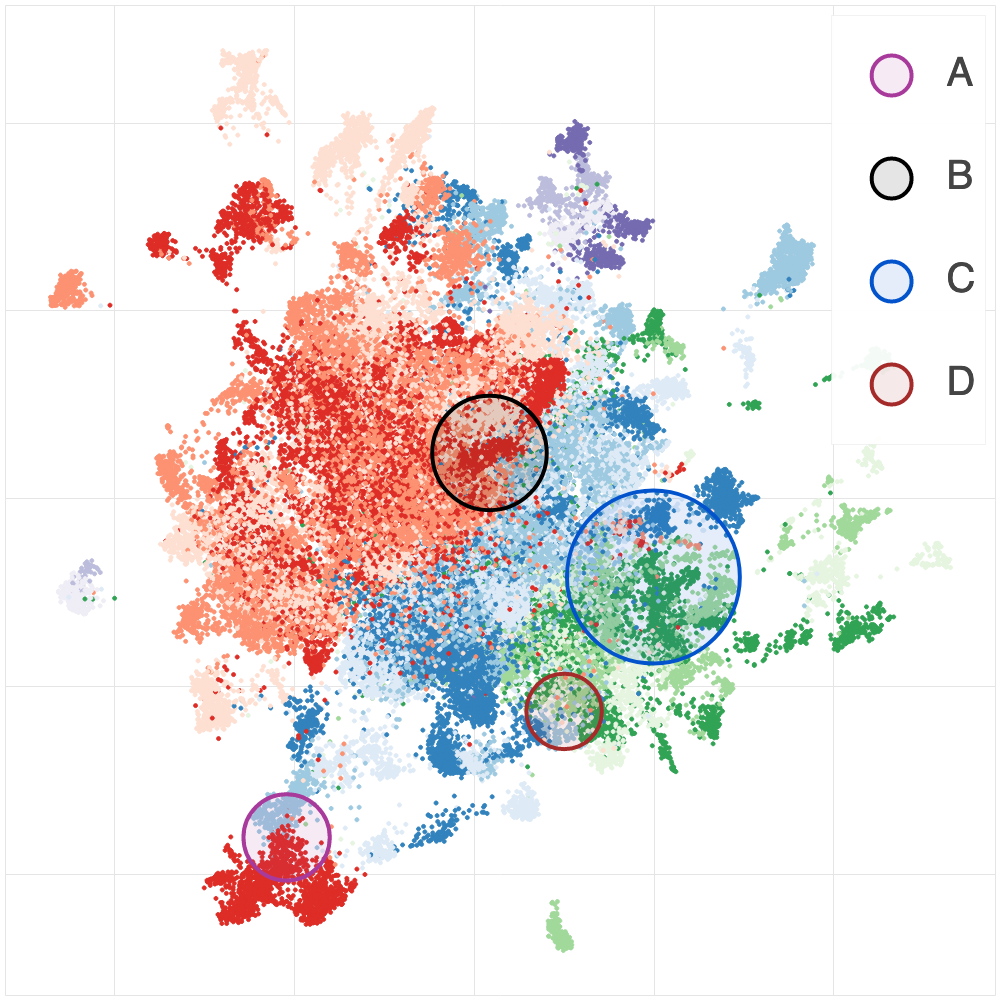
\includegraphics[width=\linewidth]{sysml/plots/cross_study.png}
    \caption{UMAP visualization of cross dataset embeddings for the top 200 authors, one hue per market. Circles denote the same user in two different markets. 
    %Each circle covers a large percentage of a users' posts over two markets
    }
    \label{fig:cross_dataset}
\end{figure}


%\noindent {\bf Migrant Analysis}
\subsection{Migrant Analysis}
%Cross-market alignment is achieved using a small sample of users matched by a high-precision heuristic (PGP key match). 
%Other heuristics (eg. shared username) can also be used as indicators of an author migrating between two markets.
To understand the quality of alignment from the episode embeddings generated by our method, we use a simple top-k heuristic: for each episode of a user, find the top-k nearest neighboring episodes from other markets, and count the most frequently occurring user among these (candidate sybil account).
Figure~\ref{fig:cross_dataset} shows a UMAP projection for T200. 
Users of each market are colored by sequential values of a single hue (i.e., reds - SR2, blues - SR, etc.).
%We select pairs of users such that for each pair $(u, v)$, $u$ is the most frequent neighbor of $v$, and $v$ is the most frequent of $u$ in the top-k neighbors ($k = 10$).
The circles in the figure highlight the top four pairs of users (top candidate sybils) with a frequent near neighbor from a different market. 
We find that each of these pairs can be verified as sybil accounts, either by a shared username (A, C, D) or by manual inspection of posted information (B).   
Note that none of these pairs were pre-matched using PGP - none were present in the high-precision matches. Thus,
\SYSMLmethodname{} is able to identify high ranking sybil matches reflecting users that migrate from one market to another.

\todo{TODO: Add additional results from Darkweb folder discussion.}

\section{Ethical Considerations}
\label{sec:sysml:ethics}
The research conducted in this study was deemed to be {\it exempt research} by the Ohio State University's Office of Responsible Research Practices, since the forum data is classified as 'publicly available'. 
Darknet forum data is readily available publicly across multiple markets~\cite{dnmArchives,munksgaard2016mixing} and we follow standard practices for the darkweb~\cite{kumar2020edarkfind} limiting our analysis to publicly available information only. 
The data was originally collected to study the prevalence of illicit drug trade and the politics surrounding such trades.


\noindent \textbf{Limiting Harm} To the best of our knowledge, the collected data does not contain leaked private information~\cite{munksgaard2016mixing}. Beyond relying on the exempt nature of the study, we also strive to take further steps for minimizing harms from our research.
In accordance with the ACM Code of Ethics and to limit potential harm, we carry out substantial pre-processing (\S\ref{sec:sysml:dataset}) to remove links, images, and keys that may contain sensitive information.  
Towards respecting the privacy of subjects, we do not connect the identity of users to any private information; our method serves only to link users across markets.
Further, in this study, we restrict our analysis to darknet markets that have been inactive for several years. 
The darknet market community has itself taken steps over the past few years to link identities of trustworthy members across market closure via development of information hubs such as Grams, Kilos, and Recon~\cite{broadhurst2021impact}. 
Our efforts aim to understand the formative years that lead towards this centralization.

\noindent \textbf{Inclusiveness} Our methods do not attempt to characterize any traits of the users making the posts. Based on our analysis, the datasets contain posts in English, German, and Italian. 
Thus, our methods may be limited in applicability and biased in performance for languages belonging to these and related Indo-European languages.  
%However, based on public publications~\cite{Noorshams2020TIESTI}, we speculate that similar efforts may already be underway at different private organizations. 
%If accepted, we will ensure that we make both our code and analyses publicly available so that our results can be replicated in a transparent fashion.

\noindent \textbf{Potential for Dual Use} Our goal is to understand how textual style evolves on darknet markets and how users on such markets may misuse them for scams and illicit activities. This digital forensic analysis can be put to good use for understanding trust signalling on these markets.
%Our Institutional Review Board while noting the exempt nature of this research  also noted, and we concur, that the potential benefits from such studies has benefits that outweigh any potential harms.
We understand the potential harm from dual use; stylometric methods could be used for the identification of users who may not want their identity to be made public, especially when they are subject of hostile governments.
We believe that making the information about the existence of such stylometric advances public and providing prescriptions for avoidance techniques (\S\ref{sec:sysml:casestudy:qualitative}) would aid users who may not know of strategies that they can use to preserve their anonymity.
Existing work~\cite{noorshams2020ties,andrews2019learning} has already expanded the use of stylometry to the open web. 
Thus, we have made the analysis of patterns that lower stylometric identifiability one focus of our case study.

%\noindent \textcolor{red}{In addition, we provide a datasheet and a model card to describe the ethical implications in an easily accessible format for potential future work so that it is cognizant of these ethical considerations.}


\section{Conclusion}
\section{Conclusion}
\label{sec:conc}
%
This work focused on the \textit{pre-deplyment} stage for building more adaptive models by incorporating \textit{adversarial testing}.
We have proposed a new transformer-based system called \URLTranSys whose goal is to predict the label of an unknown URL one which either references a phishing or a benign web page.
Transformers have demonstrated state-of-the-art performance in many natural language processing tasks, and the secnd objective of this work is to understand if these methods can also work well in the cybersecurity domain.
We demonstrated that transformers which are fine-tuned using standard BERT tasks and a BPE tokenizer also work remarkably well for the task of predicting phishing URLs.
%Instead of extracting lexical features or using CNNs kernels which span multiple characters and words, common in previously proposed URL detection models, our system used BPE tokenizers for this task. 
%Next, transformers convert the token sequence to an embedding vector which can then be used as input to a dense linear layer.
Results indicate that \URLTranSys was able to significantly outperform recent baselines, particularly over a wide range of very low false positive rates.
We also demonstrated that transformers can be made robust to novel attacks under specific threat models when we adversarially augment the training data used for training them. 

%\section*{Acknowledgements}
%\input{sections/ack}

\endinput

\chapter{Towards Robust Author Representations}
\label{chp:stylometry_extensions}

In the previous chapter, we explored the applicability of graph structure in augmenting author identification models. 
However, we were limited to generalizing across different forums and across time.
In this chapter, we will explore the applicability of models trained for author representation learning on large, clear web datasets.
We will first quantify whether such models can be used to improve author identification on darkweb forums.
Further, we will evaluate the limitations of models trained on large, clear web datasets  generalizing across time and demographics.
We will conclude this discussion with some prospective directions that utilize uncertainty quantification as a data and computationally efficient method to provide bounds on the generalization capabilities of these models.
The first part of this work was also presented as a conference talk at the Cambridge Cybercrime Centre's Sixth Annual Cybercrime Conference~\citep{maneriker2023following}.


\section{Tracking User Styles on Clear and Dark Web Forums}
\label{chp:stylometry_extensions:followingTrail}
\section{Tracking User Styles across Clear and Dark Web Forums}
\label{chp:stylometry_extensions:followingTrail}
The code to reproduce the following analysis is available on Github at the following URL:\\
 {\url{https://github.com/pranavmaneriker/ccc_darkweb_stylometry}}.

\subsection{Motivation}
\label{chp:stylometry_extensions:followingTrail:motivation}
In~\chapref{chp:sysml}, we described an architecture utilizing text CNNs~\citep{kim2014convolutional} for generating the textual component of representations for authorship attribution on darknet forums.
Recent work on generalizing authorship representations has focused on a variation of the popular sentence transformer architecture~\citep{reimers2019sentencebert}.
Specifically, \citet{riverastao2021learning} compared the transferability of author representation learning models between Amazon reviews, fanfiction short stores, and Reddit comments.
They found that in a zero-shot setting, i.e., without any addition in domain data, the models trained on Reddit data had the highest degree of generalization to new domains.
This work motivates us to explore the generalization capabilities of models trained on clear web data to darkweb forums.
We explore two research questions.
First, can we apply author representation models trained on Reddit forum data directly to Darkweb forums?
Second, can we combine data from the darkweb and clear web to build better models?

\subsection{Datasets}
\label{chp:stylometry_extensions:followingTrail:datasets}

\begin{figure}
    \centering
    \begin{subfigure}{0.9\linewidth}
       
\includegraphics[width=\textwidth,alt={Screenshot of Dread.}]{stylometryExtensions/figures/Dread} 
    \end{subfigure}
    \begin{subfigure}{0.9\linewidth}
       
\includegraphics[width=\textwidth,alt={Screenshot of Reddit.}]{stylometryExtensions/figures/Reddit} 
    \end{subfigure}
    \caption{Dark web market Dread (top) and clear web market Reddit (bottom). Dread image source:~\citet{wiki:Dread}}
    \label{fig:stylometry_extensions:followingTrail:forums}
\end{figure}

\begin{table}
    \centering
    \begin{tabular}{cccc}
        \toprule
        Dataset &  \# Authors & \# Posts & \# Subforums\\
        \midrule
        Dread & 43,629 & 294,596 & 382 \\
        The Hub & 8,243 & 88,753 & 62 \\
        Reddit-201801 & 4,413,757 & 82,531,775 & 94,945 \\
        Reddit-201912 & 7,439,040 & 126,992,546 & 155,864 \\
        \bottomrule
    \end{tabular}
    \caption{Dataset statistics prior to preprocessing for comparing LUAR on clear and dark web forums.}
    \label{tab:stylometry_extensions:followingTrail:datasets}
\end{table}

To answer the research questions, we collect datasets from both clear and dark web forums.
For the clear web, we sample data from the Pushshift Reddit corpus~\citep{baumgartner2020pushshift}.
The LUAR model is trained on Reddit data sampled from the same corpus, but collected between 2015 and 2016.
To avoid any overlap with the training data, we sample data from 2018 and 2019.
We created two datasets, one for posts sampled from January 2018 and the second for posts sampled from December 2019.
Reddit is an `omni-forum'~\citep{munksgaard2016mixing}, where users can participate in a number of subcommunities (subreddit).
The similarity between Dread and Reddit is illustrated in Figure~\ref{fig:stylometry_extensions:followingTrail:forums}.
Keeping this in mind, we focus on `omni-forums' from darkweb data.
We collected datasets provided in the CrimeBB collection~\citep{pastrana2018crimebb} and sample data from `Dread' (the dark web version of Reddit) and `TheHub'.
The data from `Dread' is collected between February 2018 and January 2020, and `TheHub' is collected between January 2014 and August 2019.
Summary statistics for the unprocessed datasets are provided in Table~\ref{tab:stylometry_extensions:followingTrail:datasets}. 
As with prior analyses from~\chapref{chp:sysml}, we assume that each username corresponds to a unique author.

\subsubsection{Characterizing Author Behaviors}
\label{chp:stylometry_extensions:followingTrail:datasets:behaviors}

\begin{figure}
    \begin{subfigure}{0.75\linewidth}
        \centering
        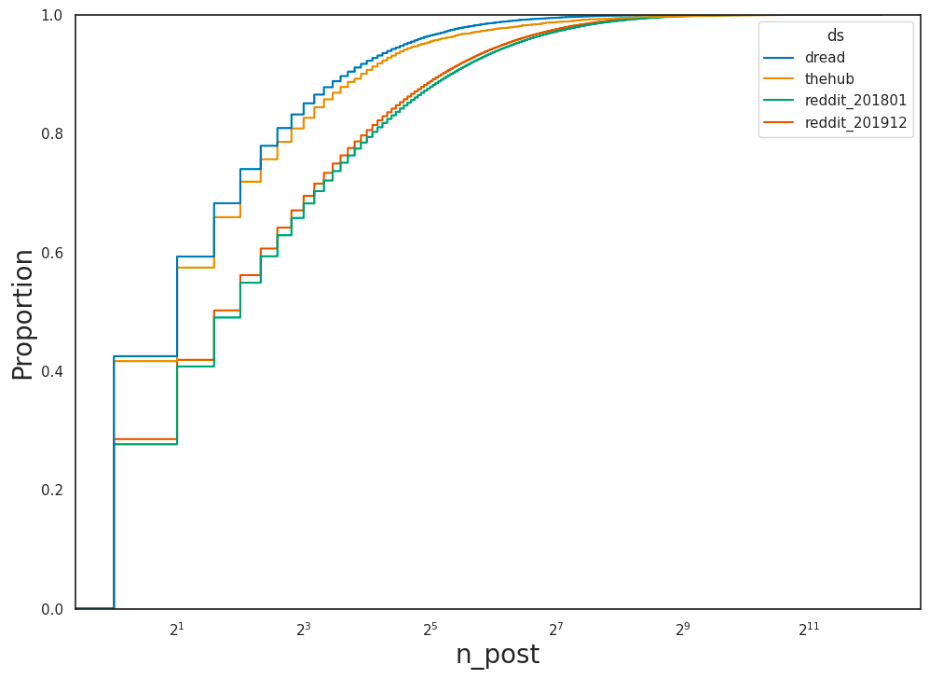
\includegraphics[width=\textwidth,alt={Empirical Cumulative Distribution Function showing the proportion of authors having n\_post posts.}]{stylometryExtensions/figures/RedditPostCDF}
        \caption{Empirical Cumulative Distribution Function showing the proportion of authors having n\_post posts. Reddit has a much smaller proportion of authors with only one post.}
        \label{fig:stylometry_extensions:followingTrail:datasets:behaviors:posts}
    \end{subfigure}
    \begin{subfigure}{0.75\linewidth}
        \centering
        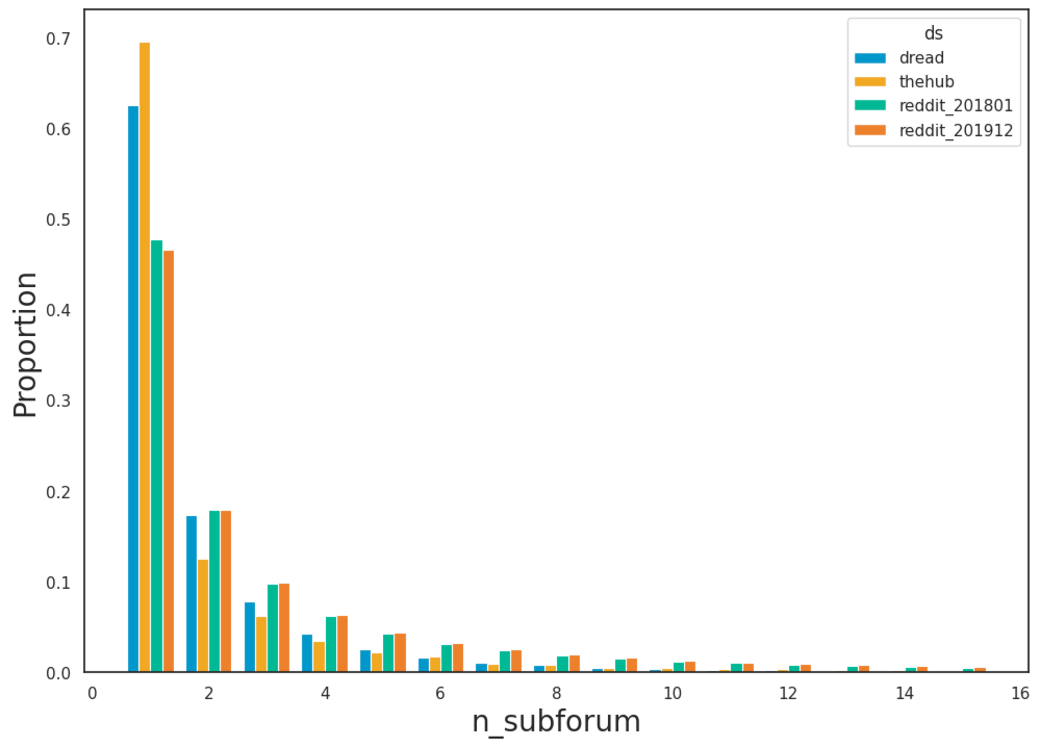
\includegraphics[width=\textwidth,alt={Histogram of the number of subforums an author has posted in.}]{stylometryExtensions/figures/RedditSubforumCounts}
        \caption{Histogram of the number of subforums an author has posted in. Reddit has fewer authors posting on only one subforum.}
        \label{fig:stylometry_extensions:followingTrail:datasets:behaviors:subforums}
    \end{subfigure}
    \caption{User behaviors on Reddit, Dread, and TheHub.}
    \label{fig:stylometry_extensions:followingTrail:datasets:behaviors}
\end{figure}

As a first step to understanding the differences in the datasets, we aim to characterize the authors.
Figure~\ref{fig:stylometry_extensions:followingTrail:datasets:behaviors} provides two figures that capture distributions that characterize the user behaviors.
Figure~\ref{fig:stylometry_extensions:followingTrail:datasets:behaviors:posts} shows the cumulative distribution function of the number of posts per author.
We observe that Reddit has a significantly smaller proportion of authors with only one post.
This indicates that there are a larger proportion of authors posting on Darkweb forums with only a single post.
This may indicate that users create \textit{throwaway accounts}~\cite{leavitt2015throwaway} more frequently on the dark web as they desire greater anonymity.
Alternatively, this may indicate that the throwaway accounts that exist on Reddit get deleted before they get captured in the intervals in-between Pushshift dataset~\citep{baumgartner2020pushshift} captures.
(Changes captured between two consecutive scrapes are not reflected in the dataset).
If an author on Reddit deletes their account, all of their posts would be reflected as posts by an author with associated username \texttt{[deleted]}.
Figure~\ref{fig:stylometry_extensions:followingTrail:datasets:behaviors:subforums} shows the histogram of the number of subforums a user has posted in.
This may indicate that either the authors on Reddit may have interests in diverse topics, or that the granularity of subforums is higher on Reddit.
Thus, even from a summary statistics perspective, there are fundamental differences in author behaviors across the clear and dark web forums.
However, it is unclear how these differences at the macro level will affect the generalization capabilities of LUAR.

\subsubsection{Preprocessing and Setup for Author Identification}
\begin{figure}
    \centering
    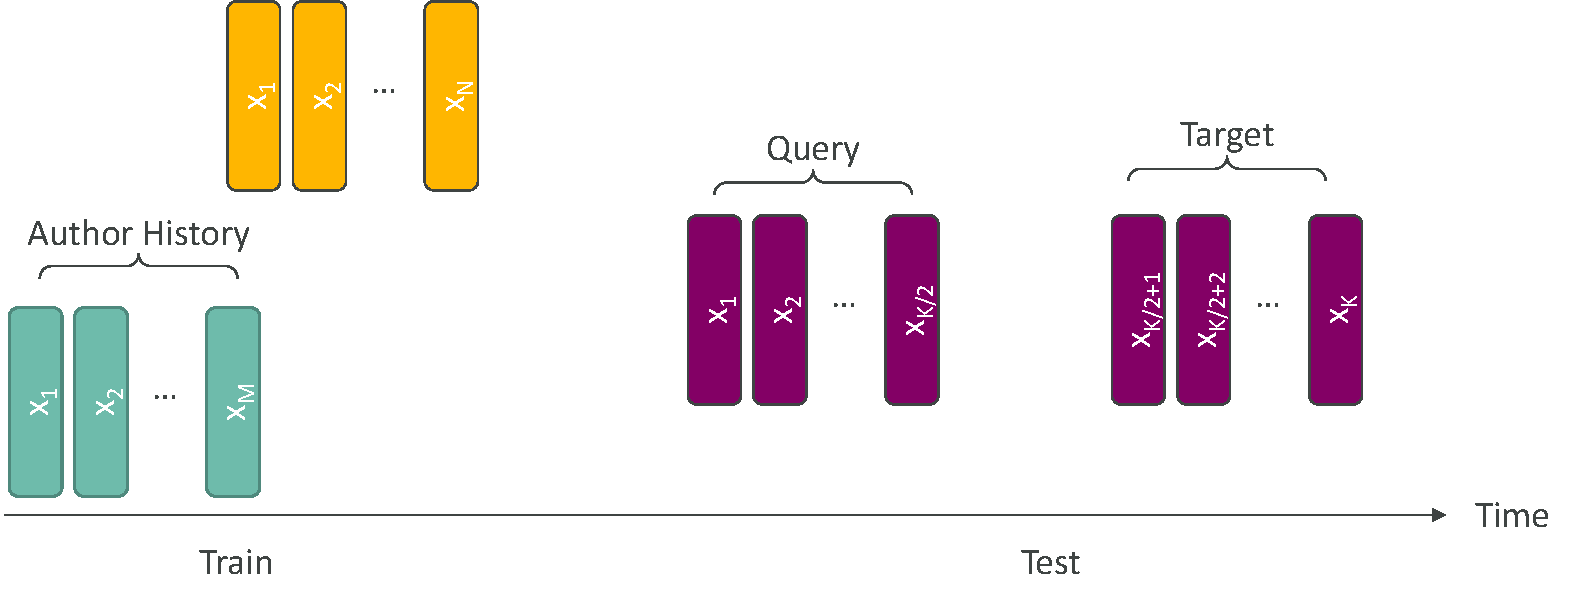
\includegraphics[width=0.9\linewidth,alt={Diagram showing how data is split for author identificaiton.}]{stylometryExtensions/figures/train_query_target_split}
    \caption{Setup of splits for the Author Identification task. Each color represents a different author.}
    \label{fig:stylometry_extensions:followingTrail:datasets:splits}
\end{figure}
We divide each dataset temporally into a 70-30 split.
That is, the first 70\% of each dataset is used for training models for experiments and the final 30\% is used for evaluation.
The evaluation set is further split into half for constructing a set of query and targets for each author.
Thus, there are three splits for each dataset labeled `train', `test\_query', and `test\_target'.
The models will be evaluated on their ability to match the representation for an author using an episode from the query set against the corresponding one in the target set.
Figure~\ref{fig:stylometry_extensions:followingTrail:datasets:splits} provides a visual representation of the setup for the author identification task. 
We filter the posts to include authors with at least 2 posts and a maximum of 1500 posts.
Further, to control for the significantly higher number of users in the Reddit datasets, we sample authors from Reddit to ensure that there is an equal number of authors in the Dread dataset and each Reddit dataset.
Figure~\ref{fig:stylometry_extensions:followingTrail:datasets:final_splits} shows the number of posts and authors in each dataset and split after preprocessing.


\begin{figure}
    \centering
    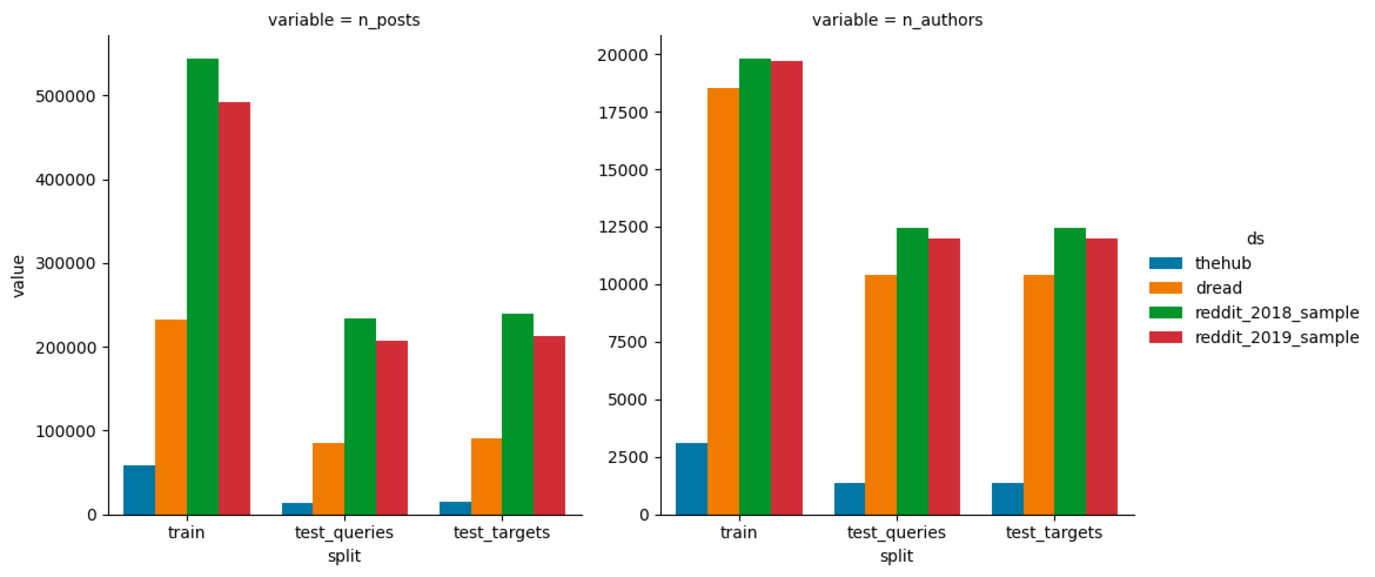
\includegraphics[width=0.9\linewidth,alt={Bar chart showing final statistics for each split.}]{stylometryExtensions/figures/FinalSplits}
    \caption{Number of authors in each dataset after preprocessing.}
    \label{fig:stylometry_extensions:followingTrail:datasets:final_splits}
\end{figure}

\subsection{Results}

For the following results, we set the episode length to 4. We consider sequence lengths (number of tokens sampled per window) at $32$ and $64$.

\subsubsection{Zero-shot Transfer}
\begin{figure}
    \centering
    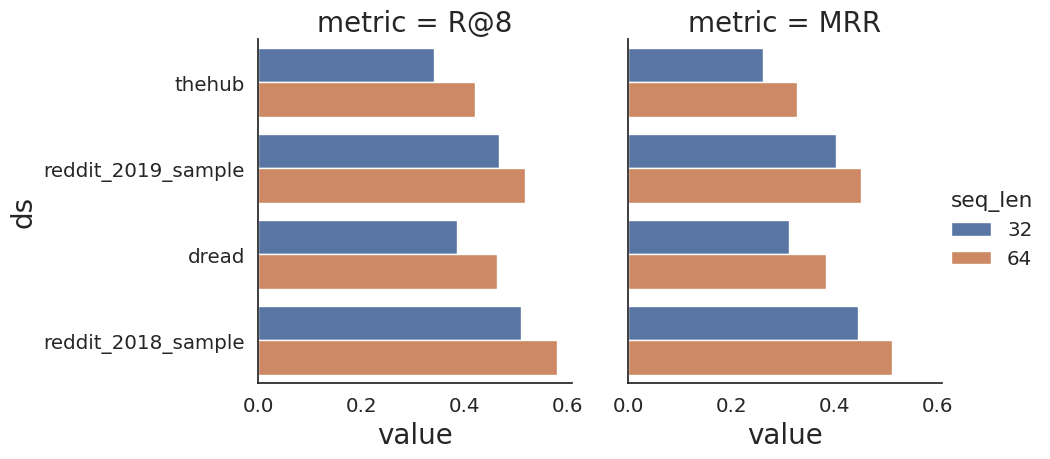
\includegraphics[width=0.9\linewidth,alt={Bar charts comparing LUAR in a zero-shot setting.}]{stylometryExtensions/figures/results/rq1_zeroshot} 
    \caption{Zero-shot performance of LUAR on the test set from Reddit-201801, Reddit-201912, Dread, and TheHub. seq\_len denotes the number of tokens sampled in each window.}
    \label{fig:stylometry_extensions:followingTrail:results:rq1_zeroshot}   
\end{figure}
We first evaluate the original LUAR model \texttt{LUAR-orig} in a zero-shot setting.
That is, we evaluate the model on the test set from the Reddit-201801 and Reddit-201912 datasets, and the Dread and TheHub datasets without any additional tuning.
Figure~\ref{fig:stylometry_extensions:followingTrail:results:rq1_zeroshot} shows the results of this experiment.
We evaluate the Recall@8 and Mean Retrieval Rank (MRR) for the LUAR model (see Section~\ref{sec:sysml:eval} for definitions of these metrics).
The results show that the LUAR model performs well on the Reddit datasets (R@8 $>0.5$ for a sequence length of $64$), but has a significant drop in performance on the Dread and TheHub datasets.
This indicates that a zero-shot transfer of the LUAR model from Reddit to Dread and TheHub is not sufficiently effective.
For the remainder of the experiments, we use the sequence length of $64$ as it provides the best performance on the Reddit datasets.

\subsubsection{Darkweb vs Clearweb Models}
\begin{figure}
    \centering
    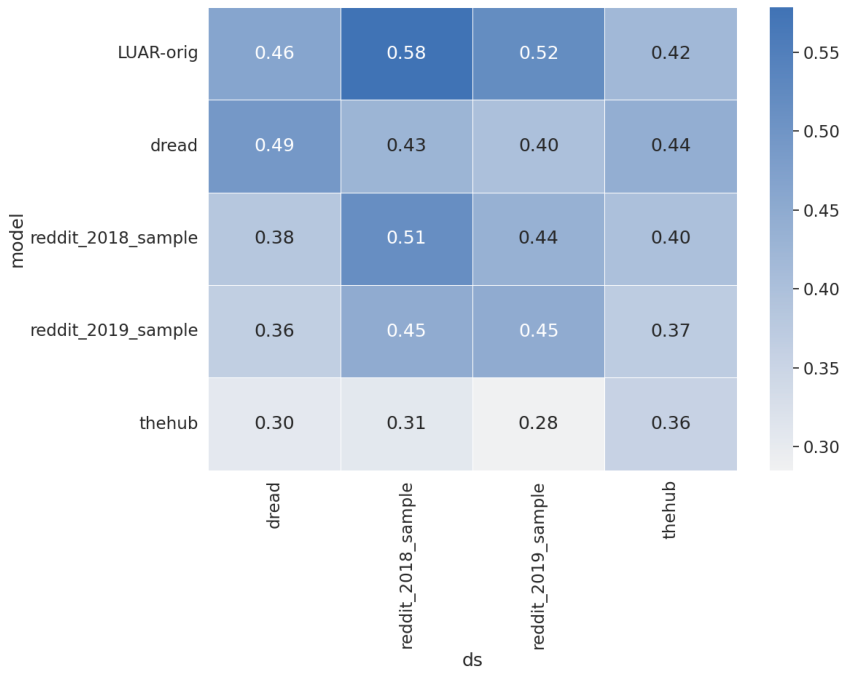
\includegraphics[width=0.8\linewidth,alt={Heatmap comparing Recall@8 across models.}]{stylometryExtensions/figures/results/rq2_trainedmodels} 
    \caption{Heatmap comparing Recall@8 across models. Each row represents the training dataset used for training the LUAR model, while each column represents the test dataset.}
    \label{fig:stylometry_extensions:followingTrail:results:rq2_trainedmodels}
\end{figure}
To better understand the impact of different datasets, we train a separate LUAR model on the training split of each of the datasets.
The heatmap in figure~\ref{fig:stylometry_extensions:followingTrail:results:rq2_trainedmodels} shows the results of this experiment.
Each row corresponds to the dataset used to train the LUAR model, and each column corresponds to the test dataset.
The first row corresponds to the results from the original LUAR model trained on one year of Reddit data.
We find that the Dread-based training dataset is significantly better than the Reddit-based training datasets for generalizing to stylometry on Darkweb data.
In fact, the performance of the model trained on Dread generalizes better to TheHub than the model trained on one full year of Reddit data.
At the same time, we note that the Dread-based model falls short of the Reddit-based models on the Reddit datasets.
This motivates us to try a hybrid approach, where we train the LUAR model on a combination of Reddit and Dread data.

\subsubsection{Hybrid Dataset: Combining Clear and Dark Web Data}
\begin{figure}
    \centering
    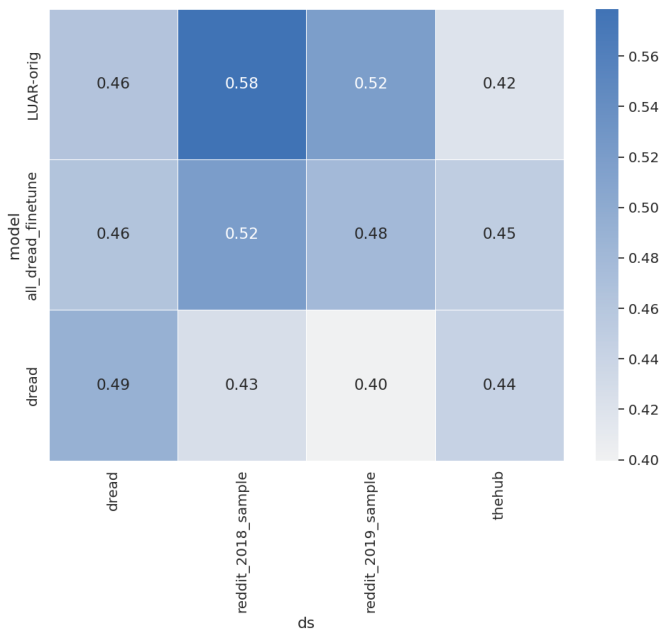
\includegraphics[width=0.8\linewidth,alt={Heatmap comparing Recall@8 with combined dataset.}]{stylometryExtensions/figures/results/rq3_combine} 
    \caption{Heatmap comparing Recall@8 across models with a combined dataset and individual datasets.}
    \label{fig:stylometry_extensions:followingTrail:results:rq3_combine}
\end{figure}

Finally, in Figure~\ref{fig:stylometry_extensions:followingTrail:results:rq3_combine}, we evaluate the performance of the LUAR model trained on a combination of Reddit and Dread data.
The R@8 for this model improves upon the R@8 of the models trained on Reddit or Dread alone in its ability to generalize to TheHub.
This supports our hypothesis that combining data from the clear and dark web can lead to better generalization capabilities for author identification models.

\subsection{Discussion}
The results of the experiments show that the LUAR model trained on Reddit data alone does not generalize well to darkweb datasets (Dread and TheHub).
However, creating a hybrid dataset by combining data from Reddit and Dread leads to better generalization capabilities.
This supports our thesis that combining data from the clear and dark web can lead to better generalization capabilities for author identification models.
Further work in this direction could explore the impact of different proportions of clear and dark web data on the generalization capabilities of author identification models.


\endinput


\chapter{Conclusions and Future Work}
\label{chp:future_work}

In this preceding chapters, we described structures that help models be more adaptive at the three different stages of their lifecycle.
Specifically, we used implicit and explicit structures along with \textit{adversarial testing}, \textit{online monitoring}, and \textit{domain adaptation} to build more adaptive machine learning systems.
We now describe some directions for extending these techniques for future work.

\pmcomment{Complete this}

\section{Large Scale Structure-aware Authorship Attribution}
\label{sec:future_work:scale}
In this extension, our goal is to test the generalizability of our findings related to the improvements offered by utilizing forum graph structures on the darkweb (Chapter~\ref{chp:sysml}).
Recent work on cross-domain authorship attribution using text has determined that certain domains (eg. Reddit) are more useful for training authorship attribution models that generalize to other domains~\cite{barlas2020cross,riverastao2021learning}.
Specifically, \citet{riverastao2021learning} demonstrate that in the source domain, diversity in the expressed topics and larger number of unique users play a role in explaining better transfer to target domains.
However, this work does not utilize the additional structure and context present in different domains.
We posit that these graphs can provide information orthogonal to that which is already present in the text.
 With our future work, we aim to demonstrate that even in scenarios with an abundance of text/users (over 100k users/1M text posts), these graph structures help improve authorship identification within a single domain, and also help better generalize across domains.
 Chapter~\ref{chp:sysml} shows that this is true in the complementary setting with fewer users ($\approx$ 1-10k)
In the remainder of this section, we first describe the choices that are involved in constructing graph structures and their similarities across domains. 
We then describe our preliminary work on utilizing these structures for authorship attribution on Reddit and share our preliminary findings.
To conclude this section, we describe additional directions that we hope to explore, including the associated datasets and techniques that help with \textit{domain generalization}.

\subsection{Graphs in Authorship Attribution}

Prior to the prevalence of neural network approaches, seminal work in computational authorship attribution~\cite{stamatatos2009survey} often used syntax-based features including, part-of-speech tags, phrase structures, and syntactic error-based features, among others.
These features may also improve neural authorship attribution models but are not the graphs focal to our analysis.
Instead, we center our work on online content platforms and identify the organizational structures that they use.
A multitude of platforms that involve individuals posting content online have associated graph structures.
We focus on structures common to platforms that face potential challenges with content moderation where authorship identification has the potential to play an important role.
%Figure~\ref*{fig:future_work:scale:graphs:ocp} demonstrates that 
While individual platforms may differ, there exists a shared, underlying, meta-structure, which can be used to identify patterns that aid in stylometric analyses across domains.
In Figure~\ref{fig:future_work:scale:preliminary:reddit_meta} we show a metagraph for a specific platform but note that the the thread-comment-user structure is shared across other platforms as well.
Additional nodes in the metagraph are specific to the platform of interest.
In the following section, we focus on a specific platform - Reddit - and utilize its structure to provide preliminary evidence for its potential.

\begin{comment}
\begin{figure}
    \centering
    \begin{subfigure}{0.48\linewidth}
    \centering
        \begin{tikzpicture}[main/.style = {draw, circle}] 
            \node[main] (1) {node};
        \end{tikzpicture}    
    \end{subfigure}
    \begin{subfigure}{0.48\linewidth}
        \centering
        \begin{tikzpicture}[main/.style = {draw, circle}] 
            \node[main] (1) {node};
        \end{tikzpicture}
    \end{subfigure}
    \begin{subfigure}{0.48\linewidth}
        \centering
        \begin{tikzpicture}[main/.style = {draw, circle}] 
            \node[main] (1) {node};
        \end{tikzpicture}
    \end{subfigure}
    \caption{Example of shared meta-structure in graph structures on Online Content Platforms}
    \label{fig:future_work:scale:graphs:ocp}
\end{figure}
\end{comment}

\subsection{Preliminary Analysis: Reddit Graph-aware Authorship Identification}

\subsubsection{Dataset}
\begin{figure}
    \begin{subfigure}{0.34\linewidth}
        \centering
        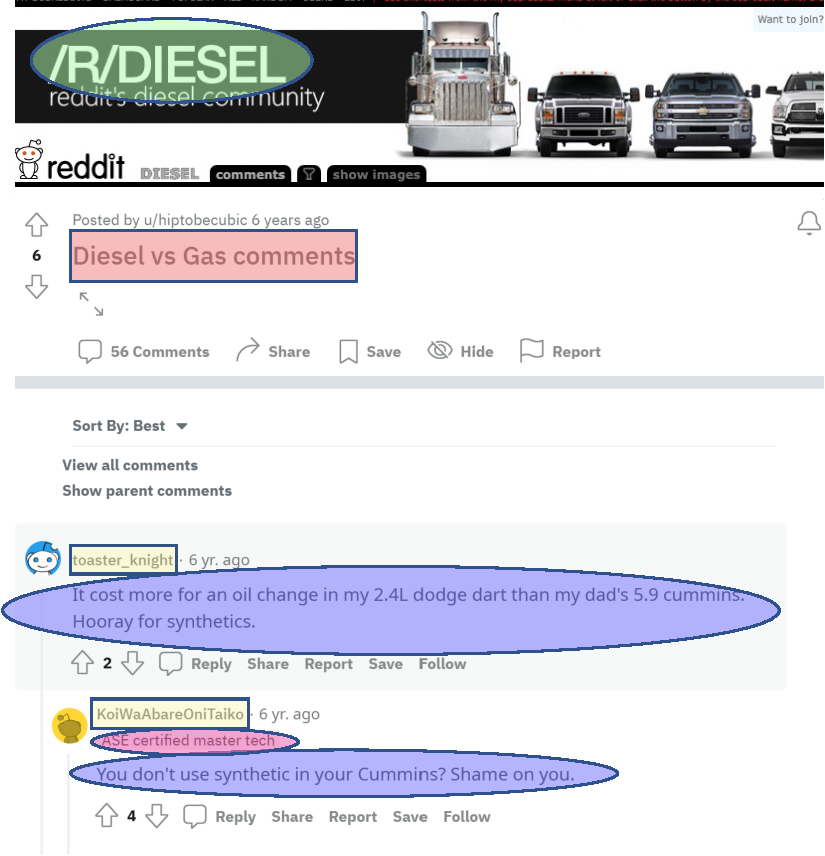
\includegraphics[width=\linewidth]{future_work/figures/reddit_metagraph.pdf}
    \end{subfigure}
    \begin{subfigure}{0.64\linewidth}
        \resizebox{\linewidth}{!}{
         \begin{tikzpicture}
            \node [ellipse,fill=green!30,line width=1.5mm] (subreddit) {Subreddit};
            \node [rectangle,fill=red!40, line width=1.5mm, below right=1cm of subreddit] (thread) {Thread};
            \node [ellipse, fill=blue!50, below right=1cm of thread] (comment) {Comment};
            \node [rectangle, fill=yellow!30,below left=0.5cm and 3cm of comment] (user) {User};
            \node [ellipse, fill=cb-rose,above left = 1cm of user] (flair) {User Flair};
            \draw[thick,<->] (subreddit) -- (thread);
            \draw[thick,<->] (thread) to[bend right] (comment);
            \draw[thick,->] (thread) to[bend left] node[fill=white] {child} (comment);
            \draw[thick,->] (comment) to[loop right] node {child} (comment);
            \draw[thick,<->] (comment) to[bend left] (user);
            \draw[thick,<->] (user) -- (flair);
            \draw[thick,<->] (flair) -- (subreddit);
        \end{tikzpicture}
        }
    \end{subfigure}
    \centering
    \caption{Metagraph of Reddit used for preliminary analysis.}
    \label{fig:future_work:scale:preliminary:reddit_meta}
\end{figure}
We collected data from a snapshot of Reddit comments over one month (Aug 2016) from the collection released by \citet{baumgartner2020pushshift}.
Figure~\ref*{fig:future_work:scale:preliminary:reddit_meta} describes the metagraph corresponding to the graph that we construct from this snapshot.
We use directed edges to distinguish comments that are direct descendants of the parent comment/thread. 
Note that the raw data collected includes only the comments posted within the month; thus, for certain comments, the text corresponding to the direct parent thread/comment may be unavailable as they are posted in the previous month. 
These comments could lead to disconnected components in the graph.
To ensure that the graph is connected, we add a bidirectional edge from each comment to the thread where it was posted.
Table~\ref*{tab:future_work:scale:preliminary:reddit_stats} shows summary statistics about the graph constructed for this dataset.

\begin{table}
    \centering
    \begin{tabular}{cc}
        \toprule
        Entity & Approximate Count \\
        \midrule 
        Subreddits &  $63,000$ \\
        Authors & $3,250,000$ \\
        Comments & $70,000,000$ \\
        Nodes & $79,100,000$ \\
        Edges & $300,000,000$\\
        \bottomrule
    \end{tabular}
    \caption{Dataset used for preliminary analysis of graphs for authorship attribution on Reddit.}
    \label{tab:future_work:scale:preliminary:reddit_stats}
\end{table}

\subsubsection{Goals}
We aim to evaluate our proposed approaches for author identification in a retrieval based setup commonly used in this setting in prior work~\cite{andrews2019learning,riverastao2021learning,khan2021deep,maneriker2021sysml}.
That is, we get a sample query text(s) and must retrieve the nearest author from a collection of target texts.
The query and target texts that the methods are evaluated on are each collected from a different time periods compared to the training set.
This ensures that the embeddings for specific authors are robust to temporal shifts.
Ensuring this is particularly challenging in the graph setting as there are multiple mechanisms to construct graphs across different time periods.
There may be authors who post in both the training, test query, and test target time periods.
In chapter~\ref{chp:sysml}, we describe one strategy where we only use subforum embeddings.
While they do provides improvements (Sec~\ref{sec:sysml:eval}), in this work we aim to incorporate further structural information.
Using the same node to denote the author in disjoint time periods would lead to a trivial embedding solution (unique node embedding for the author).
One strategy to deal with the temporal challenge is to use separate graphs for the training and testing time periods, aligning node embeddings across them.
This corresponds to the vertex nomination problem across multiple graphs, and strategies include using orthogonal procrustes~\cite{agterberg2020vertex}) for alignment.
Alternatively, node attributes such as text, time, and label could be used to construct heterogeneous, attributed graphs.
In the latter construction, certain inductive representation learning techniques for large graphs may be applied~\cite{hamilton2017inductive,xu2020inductive}.
We will now describe our initial explorations with these approaches and follow with potential future directions.

\subsubsection{Methods}
%We investigate two preliminary approaches to use the graph corresponding to the metagraph provided in Figure~\ref{fig:future_work:scale:preliminary:reddit_meta}.
\textbf{Structure-based}
\begin{figure}
    \centering
    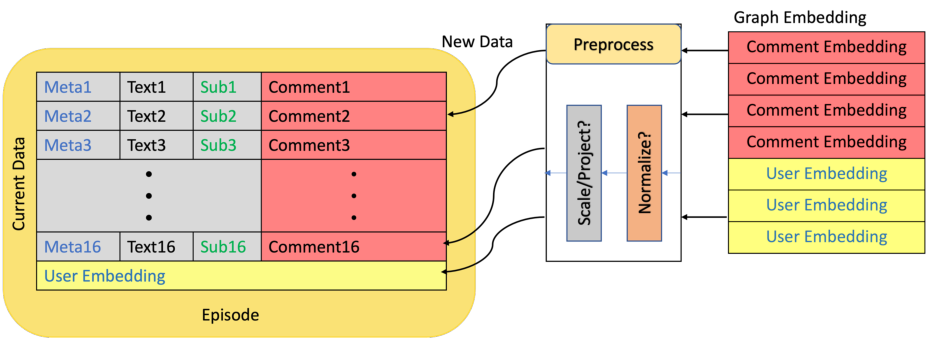
\includegraphics[width=0.9\linewidth]{future_work/figures/reddit_structure_based.pdf}
    \caption{Structure-based Author Identification Embedding}
    \label{fig:future_work:scale:preliminary:reddit_structure_embedding}
\end{figure}
In the first approach, which we designate as the \textit{structure-based} approach, we use separately generate embeddings from the structure of the Reddit graph, use a separate neural network to embed text/metadata in each episode, and then fuse the two embeddings to generate a structure-aware embedding. 
The graph embedding may need to be transformed/scaled before it is combined with the embeddings of non-graph features to ensure that their magnitudes are comparable.
Thus, we transform the embeddings prior to fusing them.
Figure~\ref{fig:future_work:scale:preliminary:reddit_structure_embedding} demonstrates the structure-based embedding approach for author identification.

\textbf{Context-based}
\begin{figure}
    \centering
    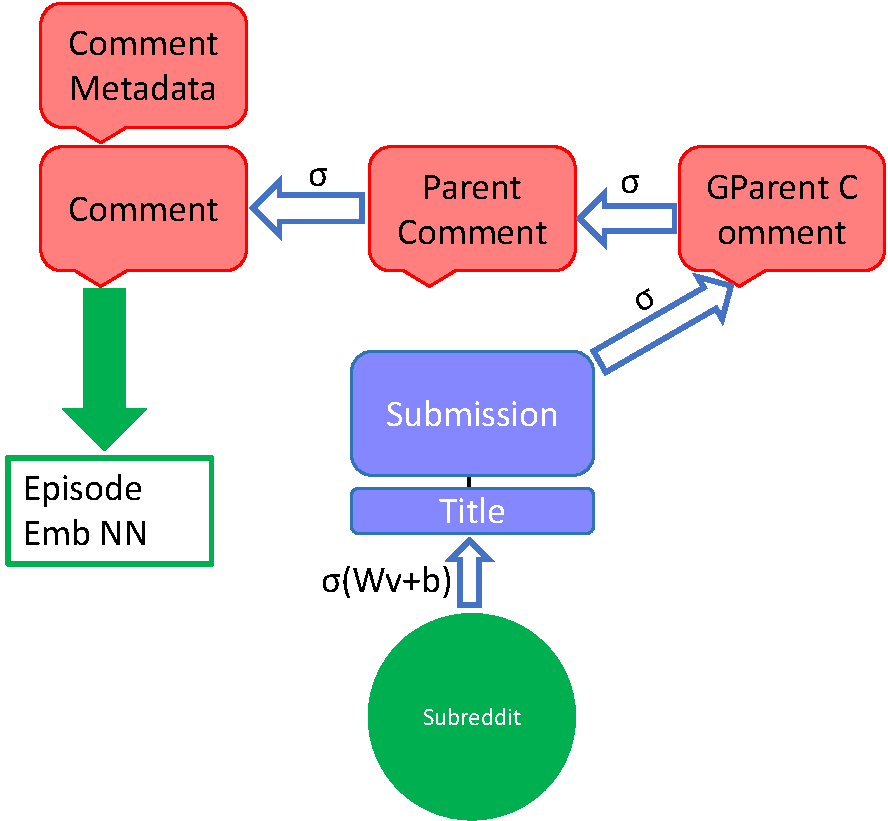
\includegraphics[width=0.5\linewidth]{future_work/figures/reddit_context_based.pdf}
    \caption{Context based Author Identification Embedding}
    \label{fig:future_work:scale:preliminary:reddit_context_embedding}
\end{figure}
The second approach, designated as the \textit{context-based} approach uses the structure of the Reddit graph to collect surrounding context for each post prior to embedding it. 
We systematically add the context from parent nodes ((grand)parent comment, thread, subreddit), each of which are individually embedded using a shared text embedding neural network.
Each layer of the architecture adds some context before applying a non-linear transformation.
Figure~\ref{fig:future_work:scale:preliminary:reddit_context_embedding} provides a  visual representation of the transformations.

\textbf{Preliminary Results}
\begin{figure}
    \centering
    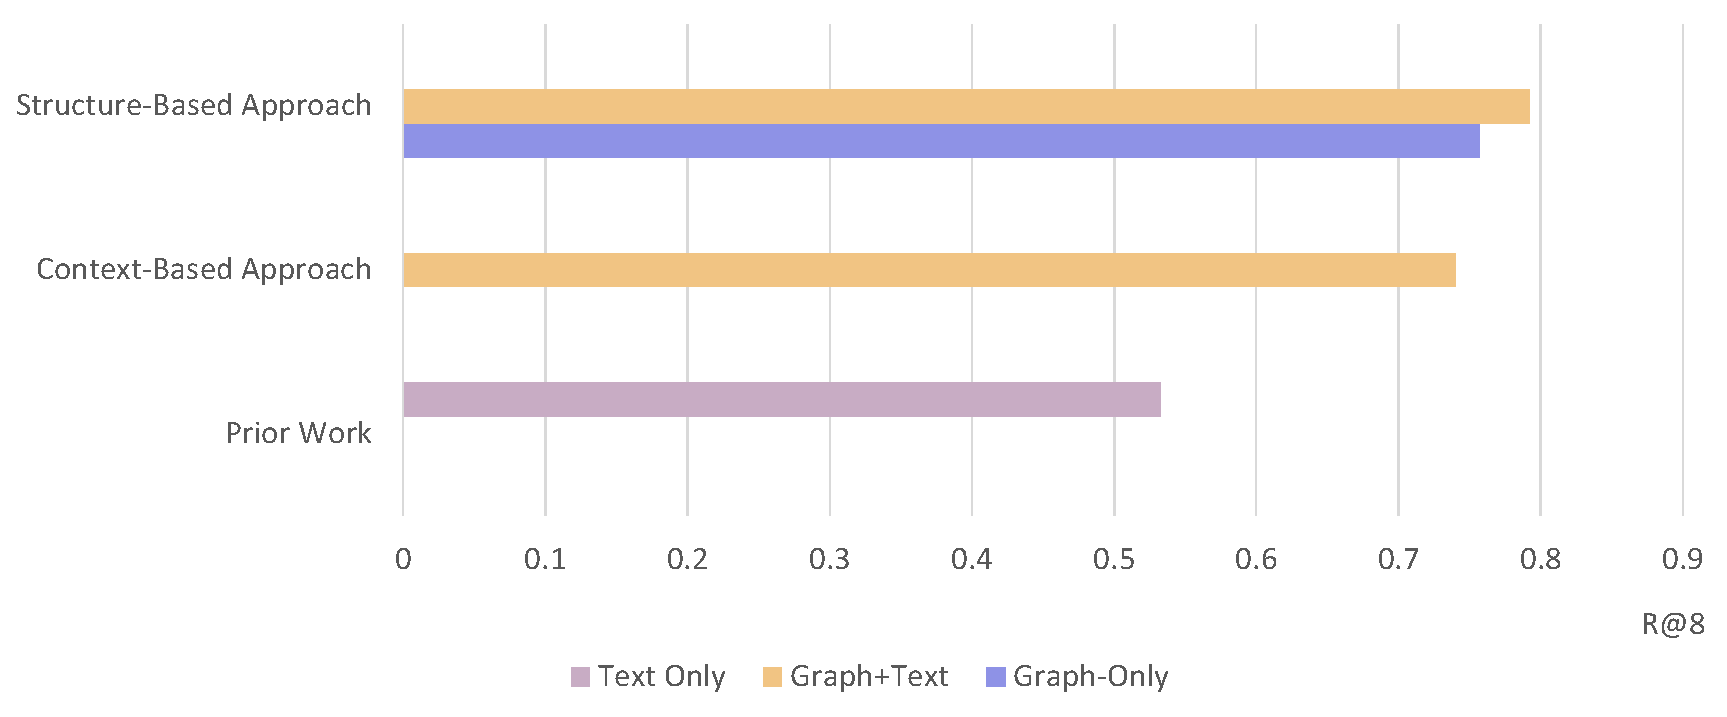
\includegraphics[width=0.8\linewidth]{future_work/figures/reddit_scale_graph.pdf}
    \caption{Results on author identification with preliminary approaches on a validation split. R@8 = recall at 8.}
    \label{fig:future_work:scale:preliminary:results}
\end{figure}
We test these approaches using SVDs of the adjacency matrix for structure-aware embeddings (à la \citet{agterberg2020vertex}) and text CNNs for embedding texts.
Figure~\ref{fig:future_work:scale:preliminary:results} demonstrates that these directions have the potential for improving author identification even on a large scale dataset.

\subsection{Future Directions}
The preliminary results are promising and demonstrate improvements over the text-based baseline.
In future work, we aim to explore the impact of alternative structure embeddings, including GNN based~\cite{velivckovic2018graph,hamilton2017inductive} and anonymous walk-based embeddings~\citep{ivanov2018anonymous,wang2020inductive}.
In particular, successes from scaling GraphSAGE-based~\cite{hamilton2017inductive,ying2018graph} approaches motivate their potential use in a hybrid fashion, where both the structure and text embeddings may be fused more effectively.
Additionally, the results in Figure~\ref{fig:future_work:scale:preliminary:results} are evaluated on a specific validation dataset.
Additional experiments need to be carried out to test whether the different stages (embedding, alignment) are affected by temporal shifts.
Finally, we aim to test the impact of using structure and context to help in better adaptation across different domains.
Specifically, we aim to test whether structure-aware embedding would adapt to authorship identification datasets from Dread (Darknet version of Reddit) and Twitter.
We will use datasets of Dread posts~\cite{pastrana2018crimebb} and Twitter posts~\cite{andrews2019learning} for these tasks.

\section{Auditing in Non-iid Settings}
\label{sec:future_work:monitoring}

In chapter~\ref{chp:avoir},  we described a confidence sequence based approach for monitoring fairness metrics associated with a decision-making function.
However, there are some assumptions underlying the derivations that allow \AVOIRmethodname{} to be used for monitoring.
In this extension, we aim to make the \AVOIRmethodname{} system more interactive, and generalize to more scenarios for more effective \textit{online monitoring}.

\subsection{Goals}
Our first goal is to make \AVOIRmethodname{} more interactive.
A user may want to change the specification that they monitor as requirements and regulations for specifications continue to evolve over time.
In the current implementation, an update of the specification requires monitoring from scratch after re-initializing all tracked expressions.
 We aim to enable more efficient modification of the monitored specification.  
The second goal is to make \AVOIRmethodname{} generalize to more diverse monitoring scenarios.
An important assumption for tracking terms in \AVOIRmethodname{} (from using the Adaptive Hoeffding inequality~\cite{zhao2016adaptive}) is that the underlying data generating process is stationary.
In the real world, this assumption may not hold.
The second assumption is the independence of decisions $y_i$ given an input $x_i$ , i.e., $y_i = f(x_i)$.
When the decision making function is based-on a non-parametric or graph-based model, this assumption may not hold.


\subsection{Datasets and Methods}
To accomplish our first goal and enable editing of specifications, we aim to implement a caching mechanism within \AVOIRmethodname{}.
We will cache the values of each \textit{elementary} subexpression and potentially certain other expressions that may help in deriving guarantees for new specifications.
In conjunction we will explore datasets and methods for fairness monitoring in non-stationary environments.
Recent work on monitoring of model performance metrics~\cite{ginart2022mldemon} test monitoring on three streaming datasets.
These include a non-stationary spam-detection dataset~\cite{katakis2005utility}, weather prediction dataset\footnote{\url{https://www.kaggle.com/datasets/jsphyg/weather-dataset-rattle-package}}, and a face detection dataset~\cite{wang2020masked}.
Along with a subset of thase and furthering our goals of exploring the non-independent decision setting, we will collect common graph datasets from SNAP~\cite{snapnets} and the Open Graph Benchmark~\cite{hu2020open}.
In terms of methods, we aim to explore recent work on improving uncertainty estimation in various non-independent and drift scenarios.
These include: black-box label shift detection~\cite{lipton2018detecting}, covariate shift~\cite{tibshirani2019conformal}, and general distribution free concentration confidence sets~\cite{howard2021time}. 
We will also contrast our setup against alternative fairness auditing mechanisms~\cite{yan2022active} that measure efficiency in terms of number of queried labels rather than the number of post-deployment observations. 

\section{Towards more robust Stylometry}

In chapters~\ref{chp:sysml} and~\ref{chp:stylometry_extensions}, we study the robustness of authorship attribution models across time and domains.
The methods we propose in chapter~\ref*{sysml} require retraining a model with additional context provided from graph-based representations.
This is because, as indicated from the results in chapter~\ref*{chp:stylometry_extensions}, the representations learned by models trained on one domain do not always generalize well to other domains.
Further, even within the same domain, the robustness of these models across time and demographics varies.
Our empirical results show that recalibration can be used to reduce the impact of these shifts on the performance of these models.
However, there are no statistically sound guarantees relating the performance of the model after recalibration.
Our success with conformal prediction in aforementioned work motivates us to use it as a tool to provide such guarantees in the context of authorship attribution.
In the final direction of proposed future work, we discuss how a conformal prediction-based approach may be used to achieve such guarantees.

\pmcomment{Pasted from earlier here}
\subsubsection{Calibration}

\DSfixeddelta{}
Steps to generate validation split for calibration:
\begin{enumerate}
    \item Select query/target from one split (We choose LUAR 1-15/12-15).
    \item Calculate all pairwise cosine similarities and sum of magnitudes.
    \item Sample a subset of users.
    \item For each user, create a data point with label 1 and score $ = cos(f(q_{u}), f(t_{u}))$, magnitude $=\norm{f(q_{u})} + \norm{f(t_{u})}$, where $f$ is the LUAR model.
    \item In addition, sample $n_{neg} = 5$ negative samples, with label 0 and score $ = cos(f(q_{u}), f(t_{u'}))$, magnitude $=\norm{f(q_{u})} + \norm{f(t_{u'})}$.
    \item Make distributional plots for these (Figure~\ref{fig:calibration:density}.
    \item Train logistic regression models which takes these (score/mag) as input and predicts the label. Create a reliability diagram for all of these models (Figure~\ref{fig:calibration:relaibility_2015}).
    \item Plot the ROC curves corresponding to these models (Figure~\ref{fig:calibration:roc_2015})
    \item Create similar reliability diagrams for other splits - marked degradation in calibration - room to improve (FIgure~\ref{fig:calibration:reliability_2016_2019})
\end{enumerate}
\begin{table}[]
    \centering
\begin{tabular}{lrrrr}
\toprule
verified ece & guo ece & em ece & year \\
\midrule
 0.000000 & 0.003675 & 0.000437 & 2015 \\
 0.000000 & 0.003591 & 0.000438 & 2016 \\
 0.000000 & 0.003645 & 0.000368 & 2017 \\
 0.000000 & 0.005089 & 0.001455 & 2018 \\
 0.003243 & 0.007548 & 0.003914 & 2019 \\
 \bottomrule
\end{tabular}
    \caption{Initial calibration results using \cite{kumar2019verified}, and calibrating a LinearSVC from sklearn}
    \label{tab:calib:init}
\end{table}

\begin{figure}[h]
    \centering
    \begin{subfigure}{0.48\linewidth}
    \centering
    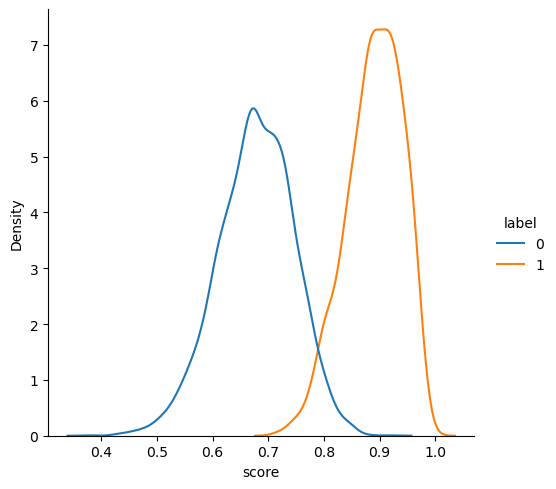
\includegraphics[width=\linewidth]{stylometryExtensions/figures/calibration_expts/cos_dist_2015.png}
    \end{subfigure} %
    \begin{subfigure}{0.48\linewidth}
    \centering
    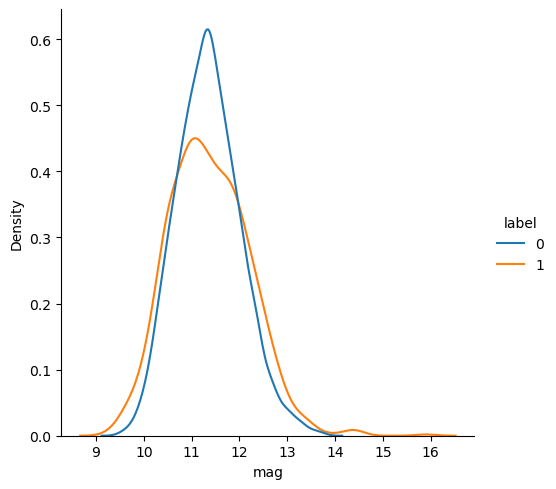
\includegraphics[width=0.5\linewidth]{stylometryExtensions/figures/calibration_expts/mag_dist_2015.png}
    \end{subfigure} %
    \caption{Density plots of cosine similarity (left) and magnitude sum (right).}
    \label{fig:calibration:density}
\end{figure}

\begin{figure}[h]
    \centering
    \includegraphics[width=0.5\linewidth]{stylometryExtensions/figures/calibration_expts/calibrate_2015.png}
    \caption{Reliability diagrams for LUAR 2015 scores.}
    \label{fig:calibration:relaibility_2015}
\end{figure}

\begin{figure}
    \centering
    \includegraphics[width=0.5\linewidth]{stylometryExtensions/figures/calibration_expts/roc_2015.png}
    \caption{ROC curve for LUAR 2015.}
    \label{fig:calibration:roc_2015}
\end{figure}


\begin{figure}
    \centering
    \includegraphics[width=0.5\linewidth]{stylometryExtensions/figures/calibration_expts/eval_calibration.png}
    \caption{Evaluating the logistic regression model calibrated on q/t in 2015 across different years.}
    \label{fig:calibration:reliability_2016_2019}
\end{figure}

\begin{comment}
\begin{figure}
    \centering
    \includegraphics[width=\linewidth]{figures/magnitude_plots/fixeddelta_mag_density.png}
    \caption{Magnitude density plots for different splits of \DSfixeddelta{} for LUAR}
    \label{fig:temporal_fixed:magnitude:density}
\end{figure}

\begin{figure}
    \centering
    \includegraphics[width=\linewidth]{figures/magnitude_plots/fixeddelta_mag_vs_n_posts.png}
    \includegraphics[width=\linewidth]{figures/magnitude_plots/fixeddelta_mag_vs_rrank.png}
    \caption{Magnitude negatively correlated with number of posts, not correlated with reciprocal rank for \DSfixeddelta{}}
    \label{fig:temporal_fixed:manitude:density_n_posts}
\end{figure}


\begin{figure}
    \centering
    \includegraphics[width=\linewidth]{figures/magnitude_plots/varydelta_mag_density.png}
    \caption{Magnitude density plot for \DSvarydelta{}}
    \label{fig:tempral_vary:magnitude:density}
\end{figure}
\end{comment}

\pmComment{TODO: Add a section summarizing conformal idea}


%
%\section{Interpretable Stylometric Modeling}
%\label{sec:future_work:interpret}
%In this direction of future work, we aim to build to improve the interpretability of representation learning models for authorship identification, including those that may use multiple modalities (such as graphs and text).
%In Section~\ref{sec:sysml:analysis}, we demonstrated the use of gradient-based methods as a preliminary approach for interpretation for the authorship identification task.
%However, unlike other common NLP tasks such as such as sentiment analysis, relation extraction, and question answering, stylometric evidence may not be directly associated with single spans of text.
%For example, the occurrence of spans having positive words/phrases may provide evidence for positive sentiment predictions by a machine learning model.
%This can be associated with a gradient-based explanation, for example, if the removal of this phrase would cause the model to change its output.
%However, in the authorship identification setting, the removal of a phrase from a single text may not be sufficient to change the output of a model since the phrase may continue to occur in a sufficient number of alternative posts created by the same author.
%Thus, in the \textit{episode}-based setup where we combine multiple posts by a single author, an explanation may be associated with a set of related modifications rather than a single removal.
%Exploring the contribution of different changes within a set provides a setup for exploiting \textit{structure} for interpretation.
%We propose two directions of exploration for future work.
%
%\subsection{Goals}
%Our goal is to generate explanations that are faithful to the model used for authorship attribution while also being useful for end uses of these models for decision making.
%In an ideal scenario, we would be privy to the proprietary tools used by various social media platforms such as \citet{reddit2020banevasion} and \citet{twitch2021banevasion} for content moderation, and also be able to access the justifications provided by humans when making these decisions.
%However, the tools and justifications are usually not publicly available.
%
%\subsection{Datasets and Methods}
%
%Due to the paucity of public datasets, we aim to study the Wikipedia Sockpuppet Investigation data~\cite{wiki2008SPI} and associated tools~\cite{smith2020wikipediaSPItools}, which  include publicly accessible justifications to understand the factors that are weighed by humans when making these decisions.
%Concurrently, we aim to game theoretic mechanisms for exploring \textit{structure} for explanations of machine learning models.
%These models~\cite{datta2016algorithmic,lundberg2017unified,sundararajan2020many,yan2021if} use Shapley values to generate attribution scores which are more suited for set-based explanations.
%Shapley values can be used to understand the weight of contributions of different elements of a set of changes in the output of the author identification models. 
%We will use the wikipedia sockpuppet datasets to understand the scope of modifications that can actually help in decision making, in conjunction with an \textit{adversarial testing} setup to study how different perturbations affect the value function for explanations.
%Training a model to learn the value function associated with an authorship identification model can help provide explanations that may be useful to end-users.
%
%
%\section{Project Schedule and Timeline}
%In Table~\ref{tab:future_work:timeline}, we define a plausible timeline over which we aim to accomplish the future work discussed in this section.
%The duration is aligned with The Ohio State University academic calendar.
%We anticipate that some of the work may roll-over into Spring 2024, contingent upon encountering roadblocks in the course of research.
%
%\begin{table}
%    \centering
%    \begin{tabular}{llcc}
%    \toprule
%        Project & Task & Priority & Duration  \\
%        \midrule 
%     \multirow{3}{*}{\ref{sec:future_work:scale}} & Structure + Alignment Approaches & High & Fall '22\\
%        & Context-based and Hybrid Approaches & High & Fall '22 - Spring '23 \\
%        & Cross domain experiments & Medium & Spring '22 \\
%    \midrule
%    \multirow{2}{*}{\ref{sec:future_work:interpret}} & Wikipedia sockpuppet data analysis & Medium & Summer '23 - Fall '23  \\
%    & Shapley value based explanations & Medium & Summer '23 - Fall '23\\
%    \midrule 
%    \multirow{2}{*}{\ref{sec:future_work:monitoring}} & Caching for better interaction & Medium & Summer '23 - Fall '23\\
%    & Non-IID uncertainity estimation & High & Spring '23 - Summer '23\\
%    \bottomrule
%    \end{tabular}
%    \caption{Plausible Project Schedule for Proposed Future Work.}
%    \label{tab:future_work:timeline}
%\end{table}

\endinput

\bibliographystyle{acl_natbib}
\bibliography{references}


\end{document}




